% !Mode:: "TeX:UTF-8"

\def\usewhat{xelatex} % 定义编译方式 pdflatex, dvipdfmx, or xelatex

\def \xuewei{Doctor} % 定义学位 Doctor or Master

\def\xueke{Engineering} % 定义学科 Engineering, Science, Management, Arts, Philosophy, Economics, Laws, Education, or History

\documentclass[cs4size,openany,twoside,UTF8,normalindentfirst,nofonts]{ctexbook}

% !Mode:: "TeX:UTF-8" 

\makeatletter
\@tempcnta=128
\loop \catcode\@tempcnta=13 \ifnum\@tempcnta<255 \advance \@tempcnta \@ne
\repeat
\makeatother

\newif\ifxueweidoctor %判断论文类型
\newif\ifxueweimaster
\def\temp{Doctor}
\ifx\temp\xuewei
  \xueweidoctortrue  \xueweimasterfalse
\fi
\def\temp{Master}
\ifx\temp\xuewei
  \xueweidoctorfalse  \xueweimastertrue
\fi

\ifxueweidoctor
  \newcommand{\cxuewei}{博士}
  \newcommand{\exuewei}{Doctor}
  \newcommand{\exueweier}{Doctoral}
  \newcommand{\xueweishort}{博}
\fi

\ifxueweimaster
  \newcommand{\cxuewei}{硕士}
  \newcommand{\exuewei}{Master}
  \newcommand{\exueweier}{Master's}
  \newcommand{\xueweishort}{硕}
\fi    % 硕博类型
% !Mode:: "TeX:UTF-8"
\usepackage{xeCJK}
\usepackage{tabularx}
\usepackage{graphicx}
\usepackage[a4paper,text={150true mm,224true mm},top=35.5true mm,left=30true mm,head=5true mm,headsep=2.5true mm,foot=8.5true mm]{geometry}
\usepackage{titlesec}               % 控制标题的宏包
\usepackage{titletoc}                   % 控制目录的宏包
\usepackage{fancyhdr}                   % fancyhdr宏包 页眉和页脚的相关定义
\usepackage{color}          % 支持彩色
\usepackage{amsmath}        % AMSLaTeX宏包 用来排出更加漂亮的公式
\usepackage{amssymb}
\usepackage[below]{placeins}%允许上一个section的浮动图形出现在下一个section的开始部分,还提供\FloatBarrier命令,使所有未处理的浮动图形立即被处理
\usepackage{flafter}       % 使得所有浮动体不能被放置在其浮动环境之前,以免浮动体在引述它的文本之前出现.
\usepackage{multirow,multicol}       %使用Multirow宏包,使得表格可以合并多个row格
\usepackage{booktabs}       % 表格,横的粗线;\specialrule{1pt}{0pt}{0pt}
\usepackage{longtable}      %支持跨页的表格。
\usepackage[hang]{subfigure}%支持子图 %centerlast 设置最后一行是否居中
\usepackage[subfigure]{ccaption} %支持双语标题
\usepackage[sort&compress,numbers]{natbib}% 支持引用缩写的宏包
\usepackage{enumitem}       %使用enumitem宏包,改变列表项的格式
\usepackage{calc}           %长度可以用+ - * / 进行计算
%\usepackage{txfonts}
\usepackage{fontspec}
\usepackage[amsmath,thmmarks,hyperref]{ntheorem}% 定理类环境宏包,其中 amsmath 选项用来兼容 AMS LaTeX 的宏包
\usepackage{etoolbox}
\AtBeginDocument{%
  \apptocmd\thebibliography{\interlinepenalty=-5000 }{}{}%
}

% 生成有书签的pdf及其开关, 该宏包应放在所有宏包的最后, 宏包之间有冲突
\def\atemp{dvipdfmx}\ifx\atemp\usewhat
\usepackage[dvipdfmx,unicode,           %dvi-->pdf 生成书签
            bookmarksnumbered=true,
            bookmarksopen=true,
            colorlinks=false,
            pdfborder={0 0 1},
            citecolor=blue,
            linkcolor=red,
            anchorcolor=green,
            urlcolor=blue,
            breaklinks=true
            ]{hyperref}
\fi

\def\atempxetex{xelatex}\ifx\atempxetex\usewhat %\def\atempxetex{xelatex} main.tex中已定义;
\usepackage[xetex,
            bookmarksnumbered=true,
            bookmarksopen=true,
            colorlinks=false,
            pdfborder={0 0 1},
            citecolor=blue,
            linkcolor=red,
            anchorcolor=green,
            urlcolor=blue,
            breaklinks=true,
            naturalnames  %与algorithm2e宏包协调
            ]{hyperref}

\defaultfontfeatures{Mapping=tex-text}
\xeCJKsetemboldenfactor{1}%只对随后定义的CJK字体有效
\setCJKfamilyfont{hei}{SimHei}
\xeCJKsetemboldenfactor{4}
\setCJKfamilyfont{song}{SimSun}
\xeCJKsetemboldenfactor{1}
\setCJKfamilyfont{fs}{FangSong}
\setCJKfamilyfont{kai}{KaiTi}
\setCJKfamilyfont{li}{LiSu}
\setCJKfamilyfont{xw}{STXinwei}
\setCJKmainfont{SimSun}
\setCJKsansfont{SimHei}
\setmainfont{Times New Roman}
\setsansfont{Arial}
\newcommand{\hei}{\CJKfamily{hei}}% 黑体   (Windows自带simhei.ttf)
\newcommand{\song}{\CJKfamily{song}}    % 宋体   (Windows自带simsun.ttf)
\newcommand{\fs}{\CJKfamily{fs}}        % 仿宋体 (Windows自带simfs.ttf)
\newcommand{\kaishu}{\CJKfamily{kai}}      % 楷体   (Windows自带simkai.ttf)
\newcommand{\li}{\CJKfamily{li}}        % 隶书   (Windows自带simli.ttf)
\newcommand{\xw}{\CJKfamily{xw}}        % 隶书   (Windows自带simli.ttf)
\newfontfamily\arial{Arial}
\newfontfamily\timesnewroman{Times New Roman}
\fi

\usepackage[plainruled,linesnumbered,algochapter]{algorithm2e}  % 算法的宏包,注意宏包兼容性,先后顺序为float、hyperref、algorithm(2e),否则无法生成算法列表
\usepackage{xltxtra}
\usepackage{listings}
\lstset{
%basicstyle=\small\ttfamily,
columns=flexible,
breaklines=true
}
\newcommand{\emultiline}[2][c]{\renewcommand{\arraystretch}{1}\begin{tabular}[#1]{@{}l@{}}#2\end{tabular} \renewcommand{\arraystretch}{1.3} }
\newcommand{\citeayu}[1]{\citeauthor{#1}~(\citeyear{#1})\citeup{#1}}

 % 引用的宏包

\graphicspath{{figures/}} %定义所有的eps文件在 figures 子目录下

\begin{document}

% !Mode:: "TeX:UTF-8" 

%\newcommand{\song}{\CJKfamily{song}}    % 宋体   (Windows自带simsun.ttf)
%\newcommand{\hei}{\CJKfamily{hei}}      % 黑体   (Windows自带simhei.ttf)
%\newcommand{\kaishu}{\CJKfamily{kai}}      % 黑体   (Windows自带simhei.ttf)

\newcommand{\yihao}{\fontsize{26pt}{26pt}\selectfont}       % 一号, 1.倍行距
\newcommand{\xiaoyi}{\fontsize{24pt}{24pt}\selectfont}      % 小一, 1.倍行距
\newcommand{\erhao}{\fontsize{22pt}{1.25\baselineskip}\selectfont}       % 二号, 1.倍行距
\newcommand{\xiaoer}{\fontsize{18pt}{18pt}\selectfont}      % 小二, 单倍行距
\newcommand{\sanhao}{\fontsize{16pt}{16pt}\selectfont}      % 三号, 1.倍行距
\newcommand{\xiaosan}{\fontsize{15pt}{15pt}\selectfont}     % 小三, 1.倍行距
\newcommand{\sihao}{\fontsize{14pt}{14pt}\selectfont}       % 四号, 1.0倍行距
\newcommand{\xiaosi}{\fontsize{12pt}{12pt}\selectfont}      % 小四, 1.倍行距
\newcommand{\wuhao}{\fontsize{10.5pt}{10.5pt}\selectfont}   % 五号, 单倍行距
\newcommand{\xiaowu}{\fontsize{9pt}{9pt}\selectfont}        % 小五, 单倍行距


%避免宏包 hyperref 和 arydshln 不兼容带来的目录链接失效的问题。
\def\temp{\relax}
\let\temp\addcontentsline
\gdef\addcontentsline{\phantomsection\temp}

\makeatletter
\gdef\hitempty{}

%重新定义BiChapter命令,可实现标题手动换行,但不影响目录
\def\BiChapter{\relax\@ifnextchar [{\@BiChapter}{\@@BiChapter}}
\def\@BiChapter[#1]#2#3{\chapter[#1]{#2}
    \addcontentsline{toe}{chapter}{\bfseries \xiaosi Chapter \thechapter\hspace{0.5em} #3}}
\def\@@BiChapter#1#2{\chapter{#1}
    \addcontentsline{toe}{chapter}{\bfseries \xiaosi Chapter \thechapter\hspace{0.5em}{\boldmath #2}}}

\newcommand{\BiSection}[2]
{   \section{#1}
    \addcontentsline{toe}{section}{\protect\numberline{\csname thesection\endcsname}#2}
}

\newcommand{\BiSubsection}[2]
{    \subsection{#1}
    \addcontentsline{toe}{subsection}{\protect\numberline{\csname thesubsection\endcsname}#2}
}

\newcommand{\BiSubsubsection}[2]
{    \subsubsection{#1}
    \addcontentsline{toe}{subsubsection}{\protect\numberline{\csname thesubsubsection\endcsname}#2}
}

\newcommand{\BiAppendixChapter}[2] % 该附录命令适用于发表文章,简历等
{\phantomsection
\markboth{#1}{#1}
\addcontentsline{toc}{chapter}{\xiaosi #1}
\addcontentsline{toe}{chapter}{\bfseries \xiaosi #2}  \chapter*{#1}
}

\newcommand{\BiAppChapter}[2]    % 该附录命令适用于有章节的完整附录
{\phantomsection 
 \chapter{#1}
 \addcontentsline{toe}{chapter}{\bfseries \xiaosi Appendix \thechapter~~#2}
}

\renewcommand{\thefigure}{\arabic{chapter}-\arabic{figure}}%使图编号为 7-1 的格式 %\protect{~}
\renewcommand{\thesubfigure}{\alph{subfigure})}%使子图编号为 a)的格式
\renewcommand{\p@subfigure}{\thefigure~} %使子图引用为 7-1 a) 的格式,母图编号和子图编号之间用~加一个空格
\renewcommand{\thetable}{\arabic{chapter}-\arabic{table}}%使表编号为 7-1 的格式
\renewcommand{\theequation}{\arabic{chapter}-\arabic{equation}}%使公式编号为 7-1 的格式

\newcommand{\algoenname}{Algo.} %算法英文标题
\newfloatlist[chapter]{algoen}{aen}{\listalgoenname}{\algoenname}
\newfixedcaption{\algoencaption}{algoen}
\renewcommand{\thealgoen}{\thechapter-\arabic{algocf}}
\renewcommand{\@cftmakeaentitle}{\chapter*{\listalgoenname\@mkboth{\bfseries\listalgoenname}{\bfseries\listalgoenname}}}

\renewcommand{\algorithmcfname}{算法}
\setlength\AlCapSkip{1.2ex}
\SetAlgoSkip{1pt}
\renewcommand{\algocf@captiontext}[2]{\wuhao#1\algocf@typo ~ \AlCapFnt{}#2} % text of caption
\expandafter\ifx\csname algocf@within\endcsname\relax% if \algocf@within doesn't exist
\renewcommand\thealgocf{\@arabic\c@algocf} % and the way it is printed
\else%                                    else
\renewcommand\thealgocf{\csname the\algocf@within\endcsname-\@arabic\c@algocf}
\fi
\renewcommand{\algocf@makecaption}[2]{%中英文双标题一定多于一行,因此去掉单行时的判断,并将\parbox中标题设置为居中
  \addtolength{\hsize}{\algomargin}%
  \sbox\@tempboxa{\algocf@captiontext{#1}{#2}}%
    \hskip .5\algomargin%
    \parbox[t]{\hsize}{\centering\algocf@captiontext{#1}{#2}}% 
  \addtolength{\hsize}{-\algomargin}%
}
\newcommand{\AlgoBiCaption}[2]{%直接取出自定义的中英文标题条目加入到真正的\caption 中  
   \caption[#1]{\protect\setlength{\baselineskip}{1.5em}#1 \protect \\ Algo. \thealgocf~~ #2} % \algoencaption{#2}   
   \addcontentsline{aen}{algoen}{\protect\numberline{\thealgoen}{#2}}
   }

\setlength{\algoheightruledefault}{1.5pt}
\newcommand{\foocaption}[1]{ \def\@algocf@pre@plainruled{\hrule height1.5pt depth0pt\kern\interspacetitleruled #1 \kern\interspacealgoruled\hrule height1pt depth0pt\kern\interspacetitleruled} }
\def\@algocf@post@ruled{\kern\interspacealgoruled\hrule height1.5pt\relax}%
\makeatother

%定义 学科 学位
\def \xuekeEngineering {Engineering}
\def \xuekeScience {Science}
\def \xuekeManagement {Management}
\def \xuekeArts {Arts}
\def \xuekePhilosophy {Philosophy}
\def \xuekeEconomics {Economics}
\def \xuekeLaws {Laws}
\def \xuekeEducation {Education}
\def \xuekeHistory {History}


\ifx \xueke \xuekeEngineering
\newcommand{\cxueke}{工学}
\newcommand{\exueke}{Engineering}
\fi

\ifx \xueke \xuekeScience
\newcommand{\cxueke}{理学}
\newcommand{\exueke}{Science}
\fi

\ifx \xueke \xuekeManagement
\newcommand{\cxueke}{管理学}
\newcommand{\exueke}{Management}
\fi

\ifx \xueke \xuekeArts
\newcommand{\cxueke}{文学}
\newcommand{\exueke}{Arts}
\fi 

\ifx \xueke \xuekePhilosophy
\newcommand{\cxueke}{哲学}
\newcommand{\exueke}{Philosophy}
\fi 

\ifx \xueke \xuekeEconomics
\newcommand{\cxueke}{经济学}
\newcommand{\exueke}{Economics}
\fi 

\ifx \xueke \xuekeLaws
\newcommand{\cxueke}{法学}
\newcommand{\exueke}{Laws}
\fi 

\ifx \xueke \xuekeEducation
\newcommand{\cxueke}{教育学}
\newcommand{\exueke}{Education}
\fi 

\ifx \xueke \xuekeHistory
\newcommand{\cxueke}{历史学}
\newcommand{\exueke}{History}
\fi 
 % 文本格式定义
% !Mode:: "TeX:UTF-8" 

\theoremstyle{plain}
\theorembodyfont{\song\rmfamily}
\theoremheaderfont{\hei\rmfamily}
\newtheorem{definition}{\hei 定义}[chapter]
\newtheorem{example}{\hei 例}[chapter]
\newtheorem{algo}{\hei 算法}[chapter]
\newtheorem{theorem}{\hei 定理}[chapter]
\newtheorem{axiom}{\hei 公理}[chapter]
\newtheorem{proposition}{\hei 命题}[chapter]
\newtheorem{lemma}{\hei 引理}[chapter]
\newtheorem{corollary}{\hei 推论}[chapter]
\newtheorem{remark}{\hei 注解}[chapter]
\newenvironment{proof}{\noindent{\hei 证明:}}{\hfill $ \square $ \vskip 4mm}
\theoremsymbol{$\square$}
\setlength{\theorempreskipamount}{0pt}
\setlength{\theorempostskipamount}{-2pt}

\allowdisplaybreaks[4]

%\CJKcaption {gb_452} 
%\CJKtilde
\setlength{\parindent}{2em}

\arraycolsep=1.6pt

\renewcommand\contentsname{\hei 目~~~~录}

\CTEXsetup[number={\arabic{chapter}}]{chapter}
\renewcommand\chaptername{第~\thechapter~章}

%\CTEXsetup[name={第,章}]{chapter}
\setcounter{secnumdepth}{4} \setcounter{tocdepth}{2}


\titleformat{\chapter}{\center\xiaoer\hei}{\chaptertitlename}{0.5em}{}
\titlespacing{\chapter}{0pt}{-5.5mm}{8mm}
\titleformat{\section}{\xiaosan\hei}{\thesection}{0.5em}{}
\titlespacing{\section}{0pt}{4.5mm}{4.5mm}
\titleformat{\subsection}{\sihao\hei}{\thesubsection}{0.5em}{}
\titlespacing{\subsection}{0pt}{4mm}{4mm}
\titleformat{\subsubsection}{\xiaosi\hei}{\thesubsubsection}{0.5em}{}
\titlespacing{\subsubsection}{0pt}{0pt}{0pt}

\titlecontents{chapter}[3.8em]{\hspace{-3.8em}\hei}{\thecontentslabel~~}{}{\titlerule*[4pt]{.}\contentspage}
\dottedcontents{section}[32pt]{}{21pt}{0.3pc}
\dottedcontents{subsection}[53pt]{}{30pt}{0.3pc}


% 按工大标准, 缩小目录中各级标题之间的缩进,使它们相隔一个字符距离,也就是12pt
\makeatletter
\renewcommand*\l@chapter{\@dottedtocline{0}{0em}{5em}}%控制英文目录: 细点\@dottedtocline  粗点\@dottedtoclinebold
\renewcommand*\l@section{\@dottedtocline{1}{1em}{1.8em}}
\renewcommand*\l@subsection{\@dottedtocline{2}{2em}{2.5em}}


% 定义页眉和页脚
\newcommand{\makeheadrule}{
\rule[7pt]{\textwidth}{0.75pt} \\[-23pt]
\rule{\textwidth}{2.25pt}}
\renewcommand{\headrule}{
    {\if@fancyplain\let\headrulewidth\plainheadrulewidth\fi
     \makeheadrule}}
\pagestyle{fancyplain}

%去掉章节标题中的数字
%%不要注销这一行,否则页眉会变成:“第1章1  绪论”样式
\renewcommand{\chaptermark}[1]{\markboth{\chaptertitlename~\ #1}{}}
\fancyhf{}

%在book文件类别下,\leftmark自动存录各章之章名,\rightmark记录节标题
%% 页眉字号 工大要求 小五
%根据单双面打印设置不同的页眉;

\ifxueweidoctor
  \fancyhead[CO]{\song \xiaowu\leftmark}
  \fancyhead[CE]{\song \xiaowu 哈尔滨工业大学\cxueke\cxuewei 学位论文}%
  \fancyfoot[C,C]{\xiaowu -~\thepage~-}
\else
  \fancyhead[CO]{\song \xiaowu 哈尔滨工业大学\cxueke\cxuewei 学位论文}
  \fancyhead[CE]{\song \xiaowu 哈尔滨工业大学\cxueke\cxuewei 学位论文}%
  \fancyfoot[C,C]{\xiaowu -~\thepage~-}
\fi

\renewcommand\frontmatter{\cleardoublepage
  \@mainmatterfalse
  \pagenumbering{Roman}}

% 调整罗列环境的布局
\setitemize{leftmargin=0em,itemsep=0em,partopsep=0em,parsep=0em,topsep=0em,itemindent=3em}
\setenumerate{leftmargin=0em,itemsep=0em,partopsep=0em,parsep=0em,topsep=0em,itemindent=3.5em}

\newcommand{\citeup}[1]{\textsuperscript{\cite{#1}}}

% 定制浮动图形和表格标题样式
\captionnamefont{\wuhao}
\captiontitlefont{\wuhao}
\captiondelim{~~}
%\captionstyle{\hang}
\hangcaption
\renewcommand{\subcapsize}{\wuhao}
\setlength{\abovecaptionskip}{0pt}
\setlength{\belowcaptionskip}{0pt}

% 自定义项目列表标签及格式 \begin{publist} 列表项 \end{publist}
\newcounter{pubctr} %自定义新计数器
\newenvironment{publist}{%%%%%定义新环境
\begin{list}{[\arabic{pubctr}]} %%标签格式
    {
     \usecounter{pubctr}
     \setlength{\leftmargin}{1.7em}     % 左边界 \leftmargin =\itemindent + \labelwidth + \labelsep
     \setlength{\itemindent}{0em}     % 标号缩进量
     \setlength{\labelsep}{0.5em}       % 标号和列表项之间的距离,默认0.5em
     \setlength{\rightmargin}{0em}    % 右边界
     \setlength{\topsep}{0ex}         % 列表到上下文的垂直距离
     \setlength{\parsep}{0ex}         % 段落间距
     \setlength{\itemsep}{0ex}        % 标签间距
     \setlength{\listparindent}{0pt} % 段落缩进量
    }}
{\end{list}}%%%%%

% 默认字体
\renewcommand\normalsize{
  \@setfontsize\normalsize{12pt}{12pt}
  \setlength\abovedisplayskip{4pt}
  \setlength\abovedisplayshortskip{4pt}
  \setlength\belowdisplayskip{\abovedisplayskip}
  \setlength\belowdisplayshortskip{\abovedisplayshortskip}
  \let\@listi\@listI}
  
% 设置行距和段落间垂直距离
\def\defaultfont{\renewcommand{\baselinestretch}{1.62}\normalsize\selectfont}
\renewcommand{\CJKglue}{\hskip 0.56pt plus 0.08\baselineskip} 
%加大字间距,使每行34个字,若要使得每行33个字,则将0.56pt替换为0.96pt。
\predisplaypenalty=0  %公式之前可以换页,公式出现在页面顶部

% 封面、摘要、版权、致谢格式定义
\def\ctitle#1{\def\@ctitle{#1}}\def\@ctitle{}
\def\cdegree#1{\def\@cdegree{#1}}\def\@cdegree{}
\def\caffil#1{\def\@caffil{#1}}\def\@caffil{}
\def\csubject#1{\def\@csubject{#1}}\def\@csubject{}
\def\cauthor#1{\def\@cauthor{#1}}\def\@cauthor{}
\def\csupervisor#1{\def\@csupervisor{#1}}\def\@csupervisor{}
\def\cassosupervisor#1{\def\@cassosupervisor{{\hei 副 \hfill 导 \hfill 师} & #1\\}}\def\@cassosupervisor{}
\def\ccosupervisor#1{\def\@ccosupervisor{{\hei 联 \hfill 合\hfill 导 \hfill 师} & #1\\}}\def\@ccosupervisor{}
\def\cdate#1{\def\@cdate{#1}}\def\@cdate{}
\long\def\cabstract#1{\long\def\@cabstract{#1}}\long\def\@cabstract{}
\def\ckeywords#1{\def\@ckeywords{#1}}\def\@ckeywords{}

\def\etitle#1{\def\@etitle{#1}}\def\@etitle{}
\def\edegree#1{\def\@edegree{#1}}\def\@edegree{}
\def\eaffil#1{\def\@eaffil{#1}}\def\@eaffil{}
\def\esubject#1{\def\@esubject{#1}}\def\@esubject{}
\def\eauthor#1{\def\@eauthor{#1}}\def\@eauthor{}
\def\esupervisor#1{\def\@esupervisor{#1}}\def\@esupervisor{}
\def\eassosupervisor#1{\def\@eassosupervisor{\textbf{Associate Supervisor:} & #1\\}}\def\@eassosupervisor{}
\def\ecosupervisor#1{\def\@ecosupervisor{\textbf{Co Supervisor:} & #1\\}}\def\@ecosupervisor{}
\def\edate#1{\def\@edate{#1}}\def\@edate{}
\long\def\eabstract#1{\long\def\@eabstract{#1}}\long\def\@eabstract{}
\long\def\NotationList#1{\long\def\@NotationList{#1}}\long\def\@NotationList{}
\def\ekeywords#1{\def\@ekeywords{#1}}\def\@ekeywords{}
\def\natclassifiedindex#1{\def\@natclassifiedindex{#1}}\def\@natclassifiedindex{}
\def\internatclassifiedindex#1{\def\@internatclassifiedindex{#1}}\def\@internatclassifiedindex{}
\def\statesecrets#1{\def\@statesecrets{#1}}\def\@statesecrets{}

% 定义封面
\def\makecover{
    \begin{titlepage}
    % 封面一
   \vspace*{0.8cm}
   \begin{center}
    \centerline{\xiaoyi\textbf\song{\cxuewei 学位论文}}

    \vspace{1cm}

    \parbox[t][2.8cm][t]{\textwidth}{
    \begin{center}\erhao\hei\@ctitle\end{center} }

    \parbox[t][5.1cm][t]{\textwidth}{ %英文标题太长时可以采用\xiaoer
    \begin{center}\erhao\textbf{\@etitle}\end{center} }

    \parbox[t][7.4cm][t]{\textwidth}{
    \begin{center}\xiaoer\textbf\song{\@cauthor}\end{center}}

    \parbox[t][1.4cm][t]{\textwidth}{
    \begin{center}\kaishu\xiaoer\textbf{哈尔滨工业大学}\end{center} }
    
    {\textbf\song\xiaoer{\@cdate}}

    \end{center}

    % 封二 空白页
    \ifxueweidoctor
      \newpage
      ~~~\vspace{1em}
      \thispagestyle{empty}
    \fi

    %内封
    \newpage
    \thispagestyle{empty}
    \pdfbookmark[0]{\@ctitle}{ctitlepage}

\begin{center}

			{\song \xiaosi
			\begin{tabular}{@{}r@{:}l@{}}
			国内图书分类号 & \@natclassifiedindex\\
 			国际图书分类号 & \@internatclassifiedindex
			\end{tabular}}\hfill
			{\song \xiaosi
			\begin{tabular}{@{}r@{:}l@{}}
			学校代码 & 10213\\
 			密级 &  公开
			\end{tabular}}
    \parbox[t][3.2cm][t]{\textwidth}{\begin{center} \end{center} }

    \parbox[t][2.4cm][t]{\textwidth}{\xiaoer
    \begin{center} {\textbf\song\@cdegree 学位论文 }\end{center} }

    \parbox[t][5cm][t]{\textwidth}{\erhao
    \begin{center} {\hei  \@ctitle}\end{center} }
	\parbox[t][9.8cm][b]{\textwidth}
     {\sihao
    \begin{center} \renewcommand{\arraystretch}{1.62} \song
    \begin{tabular}{l@{:}l}
    {\hei \xueweishort \hfill 士\hfill 研\hfill 究\hfill 生}           & \@cauthor\\
    {\hei 导\hfill 师}                       & \@csupervisor\\
	\@cassosupervisor
	\@ccosupervisor
    {\hei 申\hfill 请\hfill 学\hfill 位} & \@cdegree\\
    {\hei 学\hfill 科}           & \@csubject\\
    {\hei 所\hfill 在\hfill 单\hfill 位} & \@caffil\\
    {\hei 答\hfill 辩\hfill 日\hfill 期} & \@cdate\\
    {\hei 授予学位单位}                     & 哈尔滨工业大学
    \end{tabular} \renewcommand{\arraystretch}{1}
    \end{center} }
\end{center}

%%%%%%增加一空白页
  \ifxueweidoctor
    \newpage
    ~~~\vspace{1em}
    \thispagestyle{empty}
  \fi

    % 英文封面
    \newpage
    \thispagestyle{empty}
    \pdfbookmark[0]{\uppercase{\@etitle}}{etitlepage}

    {
    \xiaosi\noindent Classified Index: \@natclassifiedindex \\
                  U.D.C:  \@internatclassifiedindex }
    \begin{center}
    \parbox[t][1.6cm][t]{\textwidth}{\begin{center} \end{center} }
    \parbox[t][3.5cm][t]{\textwidth}{\xiaoer
    \begin{center} {  Dissertation for the {\exueweier} Degree in \exueke}\end{center} } %与中文保持一致,删除in {\exueke}

    \parbox[t][7cm][t]{\textwidth}{\erhao
    \begin{center} { \bfseries \@etitle}\end{center} }

%★★★★若信息内容不太长,不会引起信息内容分行时,使用tabular环境,否则使用下面的tabularx环境。
    {\sihao\renewcommand{\arraystretch}{1.3}
    \begin{tabular}{@{}l@{~}l@{}}
    \textbf{Candidate:}                     &  \@eauthor\\
    \textbf{Supervisor:}                    &  \@esupervisor\\
	  \@eassosupervisor
	  \@ecosupervisor
    \textbf{Academic Degree Applied for:}   &  \@edegree\\
    \textbf{Specialty:}                     &  \@esubject\\
    \textbf{Affiliation:}                   &  \@eaffil\\
    \textbf{Date of Defence:}               &  \@edate\\
    \textbf{Degree-Conferring-Institution:} &  Harbin Institute of Technology
    \end{tabular}\renewcommand{\arraystretch}{1}}

    %{\sihao\renewcommand{\arraystretch}{1.3}
    %\begin{tabularx}{\textwidth}{@{}l@{~}X@{}}
    %\textbf{Candidate:}                     &  \@eauthor\\
    %\textbf{Supervisor:}                    &  \@esupervisor\\
		%\@eassosupervisor
	  %\@ecosupervisor
    %\textbf{Academic Degree Applied for:}   &  \@edegree\\
    %\textbf{Specialty:}                     &  \@esubject\\
    %\textbf{Affiliation:}                   &  \@eaffil\\
    %\textbf{Date of Defence:}               &  \@edate\\
    %\textbf{Degree-Conferring-Institution:} &  Harbin Institute of Technology
    %\end{tabularx}\renewcommand{\arraystretch}{1}}

    \end{center}
    \end{titlepage}

%%%%%%增加一空白页
  \ifxueweidoctor
    \newpage
    ~~~\vspace{1em}
    \thispagestyle{empty}
  \fi
%%%%%%%%%%%%%%%%%%%   Abstract and keywords  %%%%%%%%%%%%%%%%%%%%%%%
\clearpage

\BiAppendixChapter{摘\quad 要}{Abstract (In Chinese)}

\setcounter{page}{1}
\song\defaultfont
\@cabstract
\vspace{\baselineskip}

\hangafter=1\hangindent=51pt\noindent
{\hei 关键词}:\@ckeywords

%%%%%%%%%%%%%%%%%%%   English Abstract  %%%%%%%%%%%%%%%%%%%%%%%%%%%%%%
\clearpage

\phantomsection
\markboth{Abstract}{Abstract}
\addcontentsline{toc}{chapter}{\xiaosi ABSTRACT}
\addcontentsline{toe}{chapter}{\bfseries \xiaosi Abstract (In English)}  
\addtocontents{toc}{\vspace{\baselineskip}}
\addtocontents{toe}{\vspace{\baselineskip}}
\chapter*{\bf Abstract}
\@eabstract
\vspace{\baselineskip}

\hangafter=1\hangindent=60pt\noindent
{\textbf{Keywords:}}  \@ekeywords
}

%%%%%%%%%%%%%%%%%%%%%%%%%%%%%%%%%%%%%%%%%%%%%%%%%%%%%%%%%%%%%%%
% 英文目录格式
\def\@dotsep{0.75}           % 定义英文目录的点间距
\setlength\leftmargini {0pt}
\setlength\leftmarginii {0pt}
\setlength\leftmarginiii {0pt}
\setlength\leftmarginiv {0pt}
\setlength\leftmarginv {0pt}
\setlength\leftmarginvi {0pt}

\def\engcontentsname{\bfseries Contents}
\newcommand\tableofengcontents{
   \pdfbookmark[0]{Contents}{econtent}
     \@restonecolfalse
   \chapter*{\engcontentsname  %chapter*上移一行,避免在toc中出现。
       \@mkboth{%
          \engcontentsname}{\engcontentsname}}
   \@starttoc{toe}%
   \if@restonecol\twocolumn\fi
   }

\urlstyle{same}  %论文中引用的网址的字体默认与正文中字体不一致,这里修正为一致的。

\renewcommand\endtable{\vspace{-4mm}\end@float}

\makeatother


\frontmatter
% !Mode:: "TeX:UTF-8" 

\newcommand{\chinesethesistitle}{局部多孔质气体静压轴承关键技术的研究} %授权书用,无需断行
\newcommand{\englishthesistitle}{\uppercase{RESEARCH ON KEY TECHNOLOGIES OF PARTIAL POROUS EXTERNALLY PRESSURIZED GAS BEARING}} %\uppercase作用:将英文标题字母全部大写;
\newcommand{\chinesethesistime}{2010 年~12 月}  %封面底部的日期中文形式
\newcommand{\englishthesistime}{December, 2010}    %封面底部的日期英文形式

\ctitle{局部多孔质气体静压轴承关键技术的研究}  %封面用论文标题,自己可手动断行
\cdegree{\cxueke\cxuewei}
\csubject{机械制造及其自动化}                 %(~按二级学科填写~)
\caffil{机电工程学院} %(在校生填所在系名称,同等学力人员填工作单位)
\cauthor{于冬梅}
\csupervisor{某某某教授} %导师名字
\cassosupervisor{副导名}%若没有,请屏蔽掉此句。
\ccosupervisor{联导名}%若没有,请屏蔽掉此句。


\cdate{\chinesethesistime}

\etitle{\englishthesistitle}
\edegree{\exuewei \ of \exueke}
\esubject{\emultiline[t]{Mechanical\\ and Automation}}  %英文二级学科名
\eaffil{School of Mechatronics Engineering}
\eauthor{Yu Dongmei}                   %作者姓名 (英文)
\esupervisor{Prof. XXX}       % 导师姓名 (英文)
\eassosupervisor{Prof. Assosuper}%若没有,请屏蔽掉此句。
\ecosupervisor{Prof. Cosuper}%若没有,请屏蔽掉此句。
\edate{\englishthesistime}

\natclassifiedindex{TM301.2}  %国内图书分类号
\internatclassifiedindex{62-5}  %国际图书分类号
\statesecrets{公开} %秘密

\iffalse
\BiAppendixChapter{摘~~~~要}{}
\fi
\cabstract{
摘要是论文内容的高度概括,应具有独立性和自含性,即不阅读论文的全文,就能获得必要的信息。
摘要应包括本论文的目的、主要研究内容、研究方法、创造性成果及其理论与实际意义。
摘要中不宜使用公式、化学结构式、图表和非公知公用的符号和术语,不标注引用文献编号。避免将摘要写成目录式的内容介绍。
}

\ckeywords{关键词~1;关键词~2;关键词~3;……;关键词~6(关键词总共~3~—~6~个,最后一个关键词后面没有标点符号)}

\eabstract{
Externally pressurized gas bearing has been widely used in the field of aviation, semiconductor, weave, and measurement apparatus because of its advantage of high accuracy, little friction, low heat distortion, long life-span, and no pollution. In this thesis, based on the domestic and overseas researching……

}

\ekeywords{keyword 1, keyword 2, keyword 3, ……, keyword 6 (no punctuation at the end) 英文摘要与中文摘要的内容应一致,在语法、用词上应准确无误。}

\makecover
\clearpage 
 % 封面

% 中英目录
\pdfbookmark[0]{目~录}{mulu}
\tableofcontents    % 中文目录
\clearpage{\pagestyle{empty}\cleardoublepage}

\ifxueweidoctor
\tableofengcontents % 英文目录
\clearpage{\pagestyle{empty}\cleardoublepage}     % 清除目录后面空页的页眉和页脚
\fi


\mainmatter\defaultfont\sloppy\raggedbottom

% !Mode:: "TeX:UTF-8" 

\BiChapter{绪论}
{Introduction}

\BiSection{课题背景及研究目的和意义}{Background, research objective and significance}

%%本课题来源于国家自然科学基金面上项目“无定型克隆代码的检测与重构方法”(批准号:61173021)。

随着计算机软件广泛应用于经济、军事、商业等各个领域中,软件质量问题日益引起了人们的广泛重视。保证软件高质量,并提高软件可理解性和可维护性已经成为软件系统开发和维护工作的一个不可或缺的重要方面。然而,随着应用需求和应用环境的不断变化,现实世界中的软件系统会随着时间而不断演化,导致了软件规模越来越大、逻辑越来越复杂,致使软件的质量、可理解性和可维护性也会随着时间逐渐的下降。其中一个重要的原因是软件系统中存在的大量的克隆代码。在软件开发和维护的过程中,代码复用作为一种常见的软件开发手段可以大大地提高软件开发效率,但是也往往会向软件系统中引入大量的克隆代码。有研究表明软件工程实践中会产生多种类型的克隆代码\cite{roy2007survey},克隆代码在大型软件系统中会占到代码总量的7-23\%\cite{baker1995finding}\cite{kontogiannis1996pattern}\cite{lague1997assessing},甚至在有的软件系统中占到59\%\cite{ducasse1999language}。

随着时间的推移和软件系统功能的不断添加,软件系统的规模越来越大,其中软件系统中的克隆代码也会越来越多,越来越多的克隆代码会使得软件变得越来越难以理解,降低了软件的可理解性。于此同时,软件中的克隆代码还会随着系统的演化并可能会发生变化,这也对软件的维护工作增加了新的挑战,降低了软件的可维护性。更进一步,克隆代码的变化也更容易导致软件缺陷,会降低软件的质量。因此,Fowler将克隆代码视为一种代码坏味(Bad Smell)\cite{fowler2009refactoring},认为克隆代码的存在会对软件系统造成不可避免的影响,从而引发了研究人员对克隆代码缺陷\cite{juergens2009code}\cite{gauthier2013uncovering}\cite{wagner2016relationship}、克隆代码有害性\cite{kapser2008cloning}\cite{selim2010studying}\cite{wang2012can}等相关研究。
%具体化?
克隆代码是影响软件质量、可理解性和可维护性的一个重要因素,如何分析和理解系统中既有的克隆代码,并对其进行有效的维护是一个值得研究的问题。目前对克隆代码的分析和维护研究已成为软件工程领域中的一个研究热点问题,同时也是亟待解决的一个问题。

为了解决克隆代码问题,研究人员对其展开了大量且深入的研究,也取得了较多的研究成果。当前对克隆代码的研究可以划分为三个主要的研究内容,即克隆代码检测研究、克隆代码分析研究和克隆代码维护研究。其中,克隆代码检测研究是最早也是研究最为充分的一个研究内容,许多克隆检测方法和工具被相继提出。截止到目前为止,研究人员已经提出和开发了许多克隆代码检测的方法和工具\cite{roy2008nicad}\cite{kamiya2002ccfinder}\cite{jiang2007deckard},可以高效且快速的识别系统中存在的多种类型的克隆代码。但由于克隆代码大量存在并且情况复杂,克隆检测结果不是完全令人满意的。目前尚没有一种检测方法能够检测出系统中所有的克隆代码,尤其是语法相似的和语义相似的克隆代码。更重要的是从系统中检测出克隆代码并不是克隆研究的最终目的,还需要对克隆代码进行分析,如克隆代码产生的原因及其对系统产生的不利影响等,从而辅助开发人员理解和维护克隆代码。因此,克隆检测仅仅是克隆代码研究的初级阶段,对克隆代码检测的研究无法消除克隆代码对软件的不利影响,更无法直接帮助提高软件的质量以及可维护性。令人值得注意的是,对克隆代码的分析和维护研究可以更好地弥补这一不足。

因此,本文通过对克隆代码的分析和维护研究,帮助维护人员理解和维护软件系统中的克隆代码,可以提高软件质量、软件可理解性和可维护性。克隆代码分析的主要目的是辅助开发人员理解克隆代码,是目前克隆代码研究中最为活跃的一个分支。经研究发现克隆代码是会随着软件演化而演化\cite{kim2005empirical}\cite{saha2011automatic},在其演化过程中克隆代码会对软件系统产生影响,同时也表现出了不同的特征\cite{gode2011frequency}\cite{mondal2012dispersion}\cite{rahman2014change}。如何深入的分析克隆代码及其演化情况,从而揭示克隆代码所隐含的信息是一个值得研究的问题。通过对克隆代码的演化分析并获取克隆代码的演化特征,对于维护人员理解克隆代码及其演化过程具有积极的意义,并进一步提高软件的可理解性。
于此同时,克隆维护研究也是克隆研究的另一项重要活动,旨在帮助维护系统中的克隆代码,帮助解决克隆代码所引发的各种问题。在克隆代码的演化过程中,往往会有相当数量代码被程序开发人员修改而发生变化\cite{krinke2007study}\cite{aversano2007clones} ,本文称之为一致性变化或者不一致变化。发生一致性变化的克隆代码会对软件系统产生较大的影响:首先确认克隆代码是否需要一致性变化和执行克隆代码的一致性变化会增加软件维护代价;而遗忘克隆代码的一致性变化也会导致克隆缺陷的产生\cite{juergens2009code}\cite{wagner2016relationship},将会进一步导致软件维护代价的增大。因此,如何避免和预测需要一致性维护的克隆代码是另一个值得研究的问题。通过预测克隆代码的一致性维护需求,可以有效的避免一致性缺陷,也可以降低克隆代码所导致的代价,并进一步帮助提高软件质量和可维护性。

基于以上分析,针对大型软件系统对软件可靠性要求较高的实际应用背景和需求,本文研究基于机器学习的克隆代码分析与一致性维护方法,帮助软件开发人员理解和维护软件系统中的克隆代码。具体来说,本文首先结合聚类分析和克隆演化的研究成果,研究并提取了克隆代码演化特征分析,揭示软件系统的克隆代码隐含的信息。然后针对克隆代码一致性变化所导致的缺陷以及额外的维护代价问题,基于贝叶斯网络分别在克隆代码创建之时和克隆代码变化之时预测克隆代码的一致性维护需求帮助维护克隆代码,可以有效地降低克隆代码维护代价和避免克隆一致性缺陷。最后结合软件开发过程,将克隆一致性需求维护预测扩展到其它的机器学习方法上,并帮助软件开发人员在软件开发时选择合适和预测模型和预测时间。因此,本文方法对于提高软件质量,使软件更易于理解和维护,不仅具有重要的科学理论意义,还具有重要的实际应用价值。


\BiSection{国内外研究现状及其分析}
{Related Work}

研究结果表明系统中通常存在着大量的克隆代码,比其例大约在为7-23\%左右,有的甚至高达59\%。克隆代码(简称克隆)是根据某种相似性的定义彼此相似的代码片段\cite{roy2007survey}。%导致克隆代码产生的原因是多种多样的,最常见的形式是通过复制粘贴操作复用已有的代码。长期存在于系统中的克隆代码,不仅影响着系统的可维护性,也影响着系统的可理解性。因此,对克隆代码的维护需求引发了一系列关于克隆代码的研究,包括克隆检测、克隆分析、克隆维护与管理等。
目前,使用最为广泛的一种克隆代码分类方法是按照克隆代码的语法和语义对克隆代码的相似程度进行定义和分类\cite{koschke2007survey},将克隆代码划分为如下四种类型:
\begin{itemize}
\item {Type-1克隆代码:除空格、格式和注释外,是完全相同的代码片段(简称1型克隆)。}
\item {Type-2克隆代码:除标识符、常量、类型外,是语法结构相同的代码片段(简称2型克隆)。}
\item {Type-3克隆代码:拷贝粘贴后修改的代码片段,如改变、增加或删除少量语句的代码,是语法结构相似的代码片段(简称3型克隆)。}
\item {Type-4克隆代码:执行相同的功能,但使用不同的语法结构实现的代码片段,是语义相似的代码(简称4型克隆)。}
\end{itemize}

其中,Type-1克隆也称为精确克隆,Type-2和Type-3克隆也称为近似克隆,前三类克隆代码是属于语法相似的克隆代码。Type-4克隆是语义相似的克隆代码。


\BiSubsection{研究热点与趋势}
{Research Hot-spots and Trends}

克隆代码研究一直以来都是软件工程领域的一个热点问题,迄今为止已有超过20年的研究时间。在此期间,研究人员发表了大量的学术论文,取得了较多的研究成果。为方便研究人员查阅相关研究,截止到2013年阿拉巴马大学一直维护着一个克隆代码领域的文献库\footnote{ http://students.cis.uab.edu/tairasr/clones/literature/ 阿拉巴马大学关于克隆代码研究的文献库。该文献库更新至2013年,目前已停止维护。} 。该文献库收录包括学术论文、技术报告以及学位论文在内的353篇文献,并按照研究内容和目标将克隆代码研究划分为以下四个研究方向:

\begin{itemize}
\item 
克隆检测方向:该方向目录下列出了与克隆代码检测相关的研究内容,旨在使用不同的方法从系统中检测出克隆代码。
\item 
克隆分析方向:该方向目录下列出了与克隆代码分析相关的研究内容,旨在帮助程序开发人员分析系统中存在的克隆代码,从而理解克隆代码。
\item 
克隆维护与管理方向:该方向目录下列出了与克隆代码维护与管理相关的研究内容,旨在通过各种技术手段维护和管理系统中的克隆代码。
\item 
综述和工具评估方向:该方向目录下列出了克隆代码综述和克隆检测工具评估相关的研究内容。
\end{itemize}

\begin{figure}[htbp]
\centering
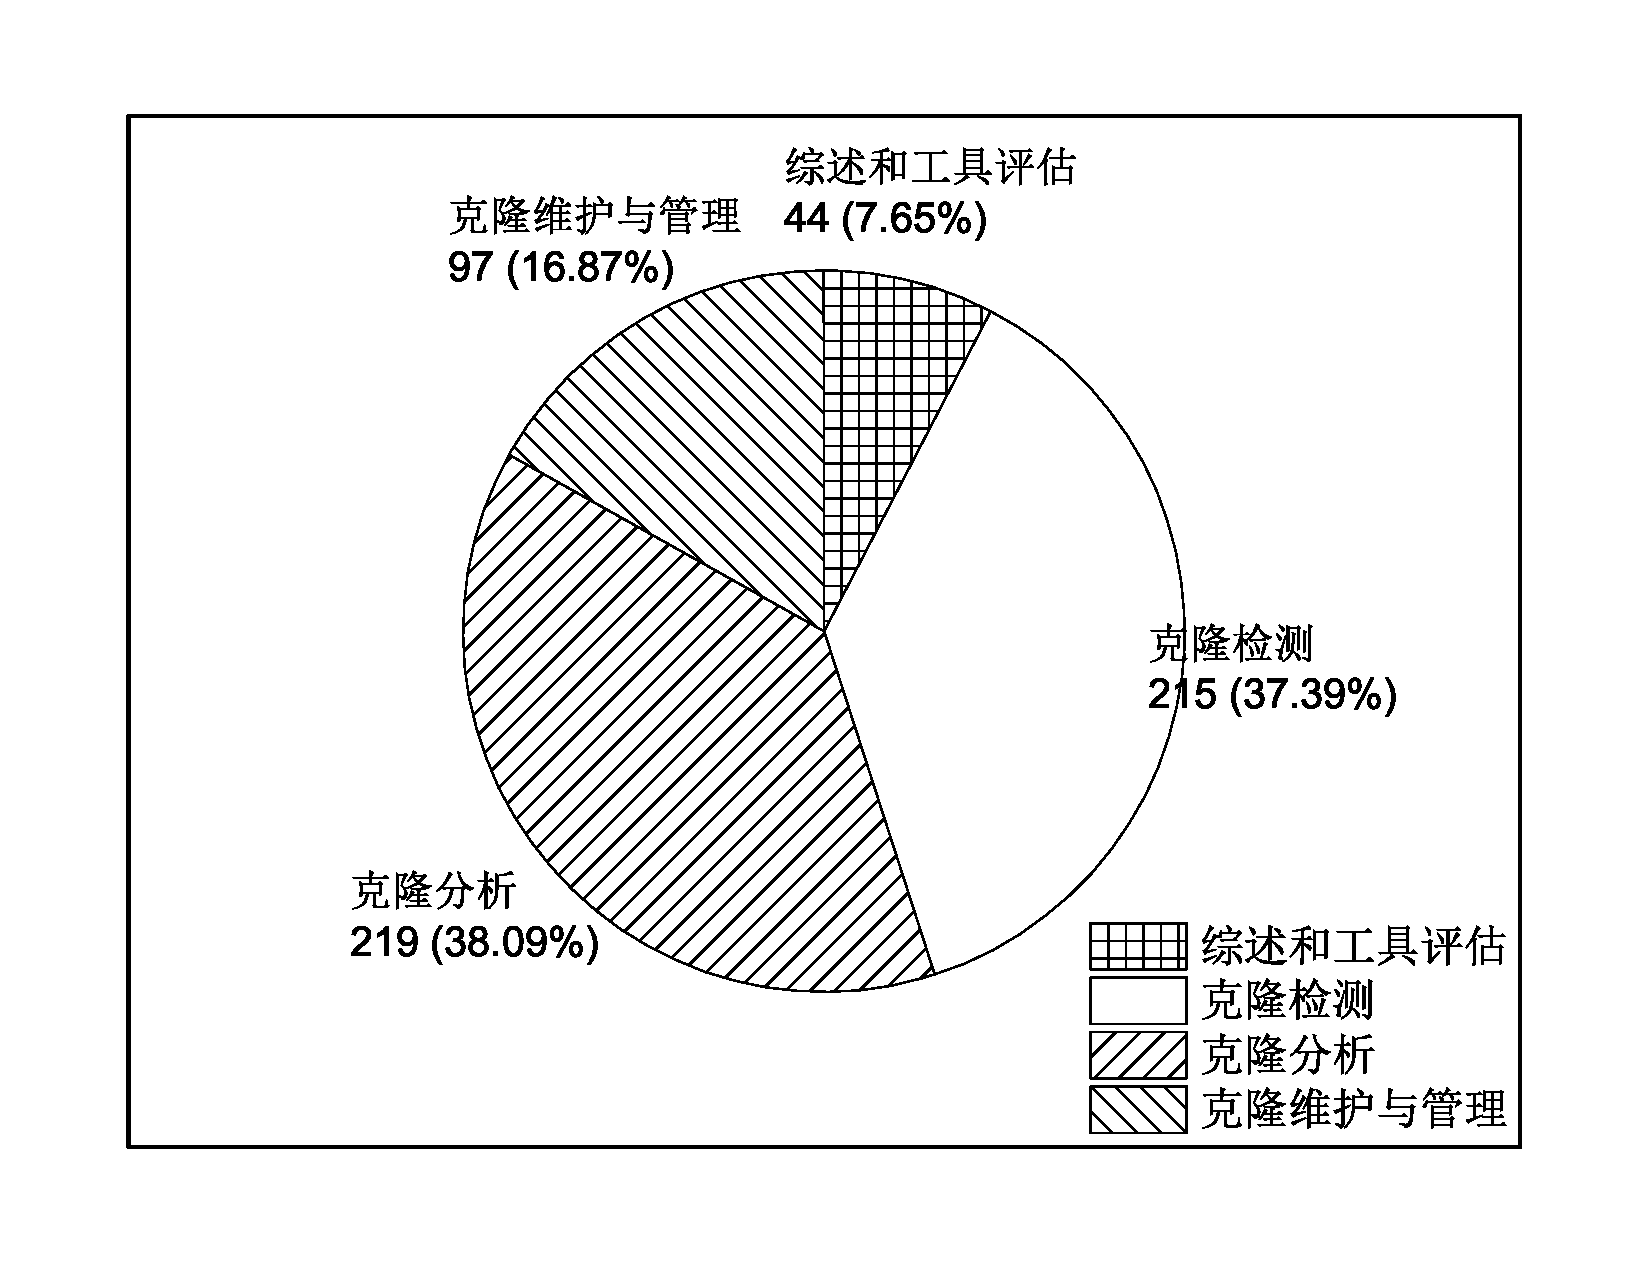
\includegraphics[width = 0.8\textwidth]{literaturedistribution1}
\bicaption[literaturedistribution1]{}{克隆代码研究领域文献分布}
{Fig.$\!$}{Literature distribution of code clone research}
%{Fig.$\!$}{Literature Distribution of Code Clone Research}
\vspace{-1em}
\end{figure}

根据此文献库中所给出的论文,Roy按照其分类进行了统计分析,分析了每个研究方向的论文分布情况和研究进展\cite{roy2014vision}。但是该文献库仅收录了2013年以前的文献,为了分析和反映克隆代码研究的最新进展、研究热点和发展趋势,本文在该文献库的基础上做了进一步的扩展,检索和收集了近几年的克隆代码相关文献,并按该文献库分类方式进行了重新统计和分析。本文统计和收集的文献共分为三类,即软件工程领域的重要国际会议论文、重要国际期刊论文以及相关学位论文。其中,重要国际会议论文为432篇,期刊论文113篇,学位论文30篇,共计575篇\footnote{本文统计的所有文献可分为两个部分:一是来源于阿拉巴马大学的文献库,二是笔者在进行研究期间所阅读整理和收集的文献。在收集的过程中,已经对文献进行了初步筛选,仅选取了领域内权威期刊、会议以及学位论文。} 。

克隆代码研究领域的文献统计分析结果如图~\ref{literaturedistribution1}~所示。从图中可以看出,目前研究中对克隆检测与分析的研究较为充分,是克隆研究领域的研究热点问题,分别占比37.39\%和38.09\%;而克隆维护与管理的研究论文占比较少(占16.87\%),说明目前对该方向的研究还方兴未艾。克隆综述和工具评估方面的研究占比更少,仅为7.65\%,说明目前较为实用的工具还不够充分。

\begin{figure}[htbp]
\centering
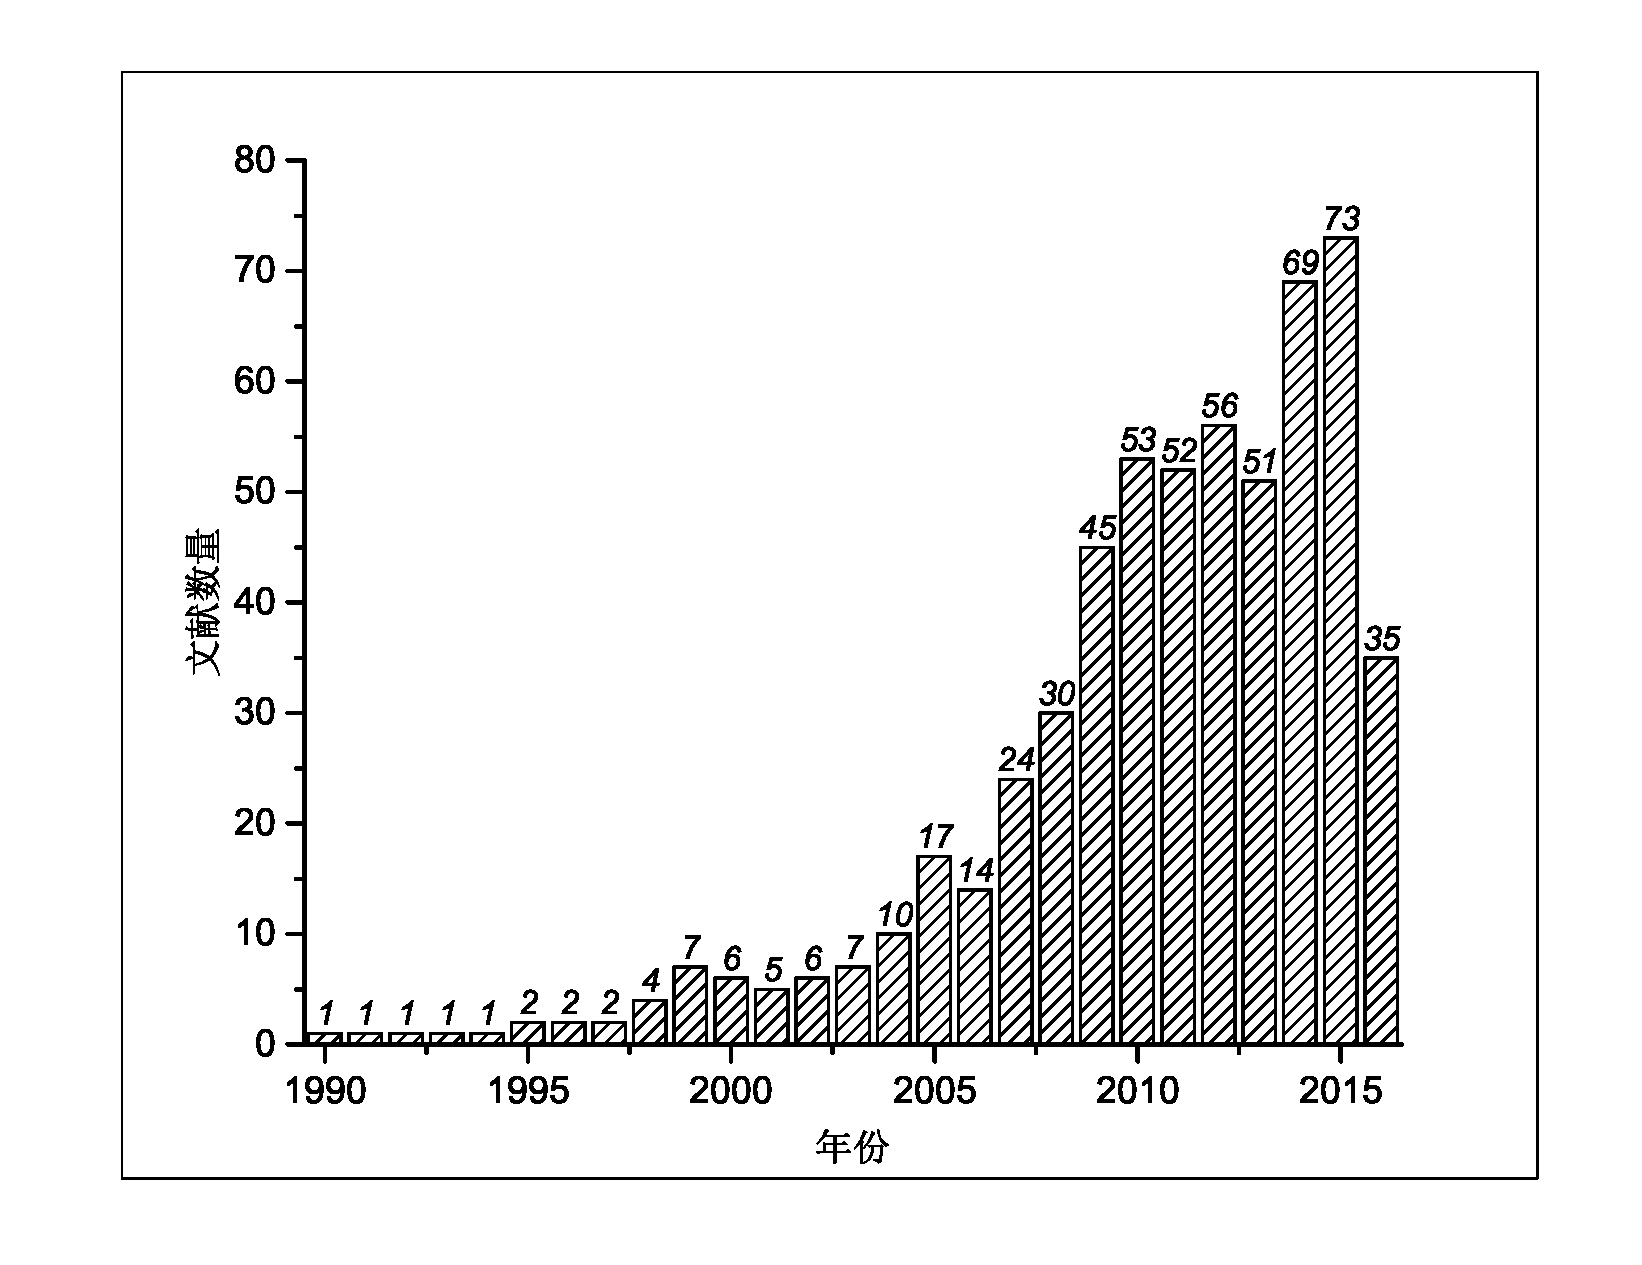
\includegraphics[width = 0.8\textwidth]{literaturedistribution2}
\bicaption[literaturedistribution2]{}{克隆领域每年发表的论文数量}
{Fig.$\!$}{Annual number of published papers of code clone research}
{Fig.$\!$}{Annual Number of Published Papers of Code Clone Research}
\vspace{-1em}
\end{figure}

\begin{figure}[htbp]
\centering
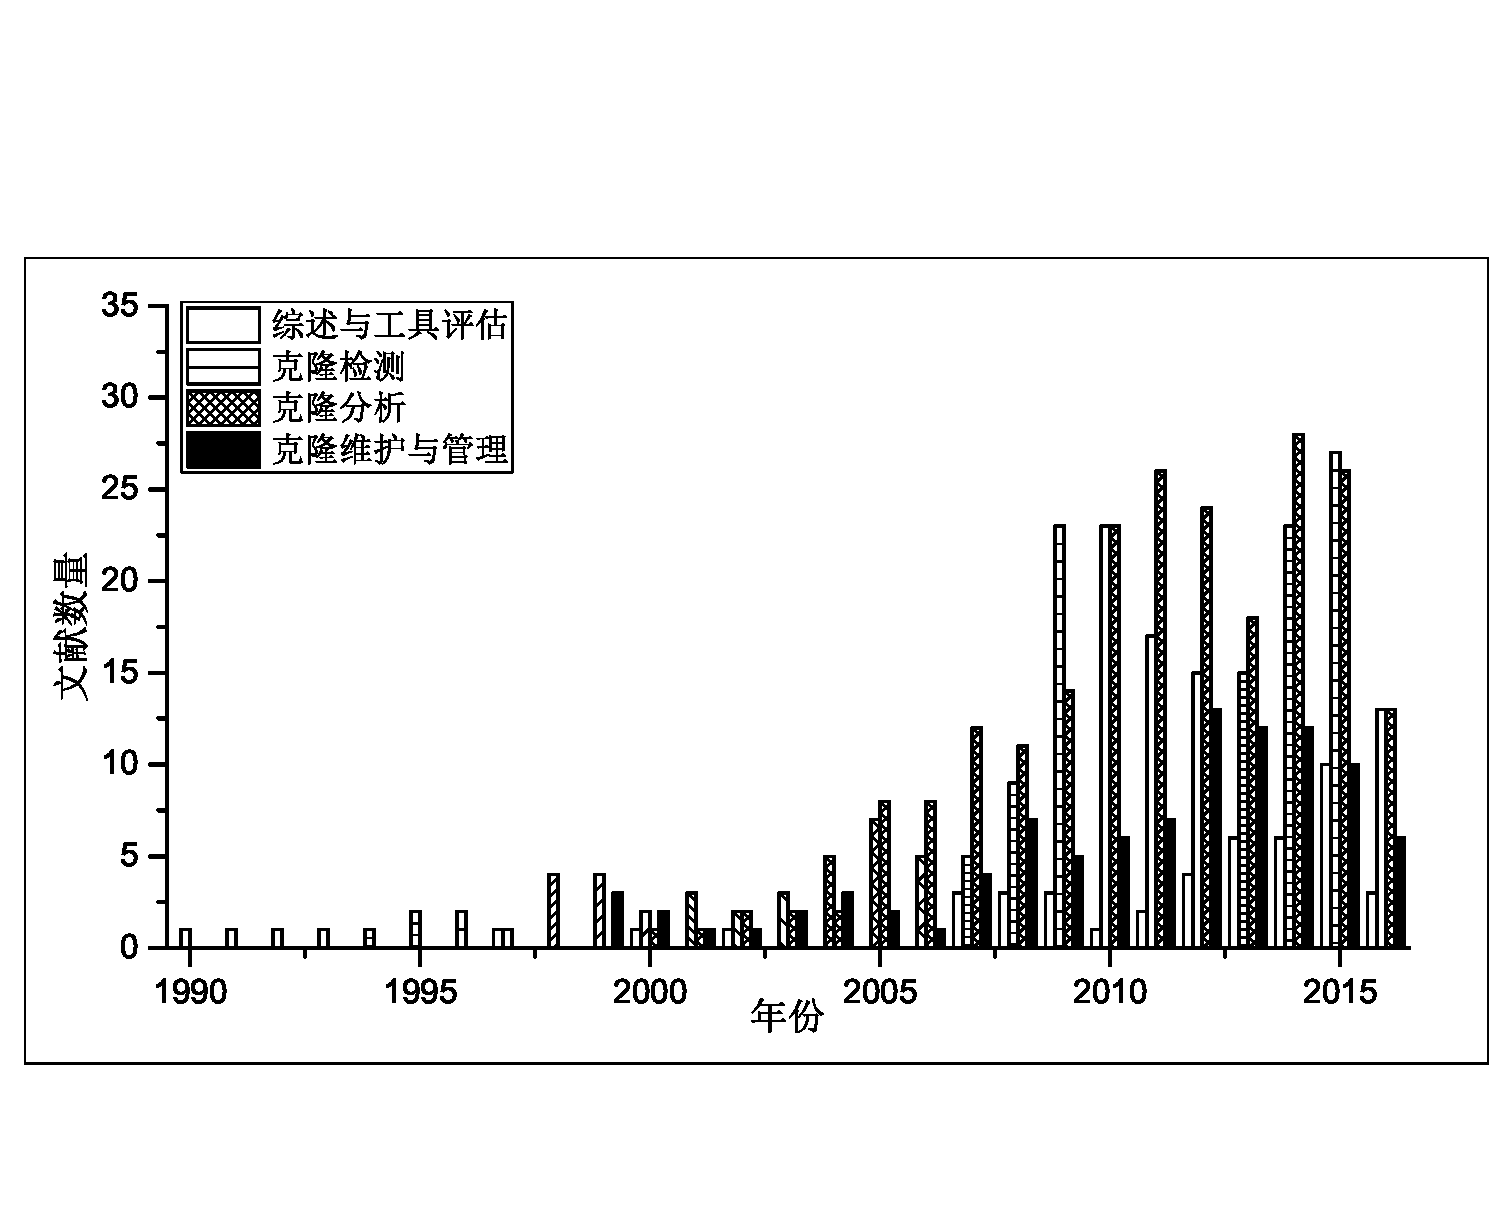
\includegraphics[width = 0.8\textwidth]{literaturedistribution3}
\bicaption[literaturedistribution3]{}{各个克隆研究活动每年发表的文献数量}
{Fig.$\!$}{Annual number of published papers of each clone research activity}
%{Fig.$\!$}{Annual Number of Published Papers of Each Clone Research Activity\vspace{-1em}
\end{figure}


为便于分析克隆代码研究领域的发展趋势,本文又对克隆代码研究领域的文献按照发表年份和研究方向进行了统计。统计分析结果如图~\ref{literaturedistribution2}~和~\ref{literaturedistribution3}~所示,其中图~\ref{literaturedistribution2}~是领域整体上每年发表文献数量的统计情况,图~\ref{literaturedistribution3}~是在不同研究方向上每年发表文献数量的统计情况。

从图~\ref{literaturedistribution2}~可以看出,克隆研究可以划分为两个阶段:1990-2003年和2004-2016年。在2003年以前,克隆代码研究领域的文献数量较少,这一阶段是克隆代码研究的孕育期。而在2004年以后的近10年内,克隆代码研究领域的文献数量快速增长,并且保持在一个较高的水平上,展现出了蓬勃的发展趋势,表明此阶段是克隆代码研究的发展期。与图~\ref{literaturedistribution2}~类似,从图~\ref{literaturedistribution3}~在不同研究方向上每年发表的文献数量来看,其研究趋势也以2003年为界限划分为两个阶段。在2003年以前,克隆代码研究主要集中在克隆检测方向,处于孕育期。在2004年以后,各个研究方向的文献数量都有了快速增长,进入了发展期。其中尤以克隆检测和分析方向的发展最为迅速,发表了大量研究成果,并依然有继续增长的趋势,说明克隆检测和分析事目前研究最为充分和最为活跃的研究方向。相比之下,克隆维护和管理仅在近几年才引起人们的关注,对克隆维护和管理的研究虽然近几年才刚开始起步,文献数量占比相对较少,但已呈现出逐年增长和后来者居上的趋势,说明克隆维护和管理正在逐渐成为克隆代码研究领域的新热点。

%\begin{figure}[htbp]
%\centering
%\subfigure{\label{literaturedistribution21}}\addtocounter{subfigure}{-2}
%\subfigure[Clone number of papers published each year in the field]{\subfigure[克隆领域每年发表的论文数量]{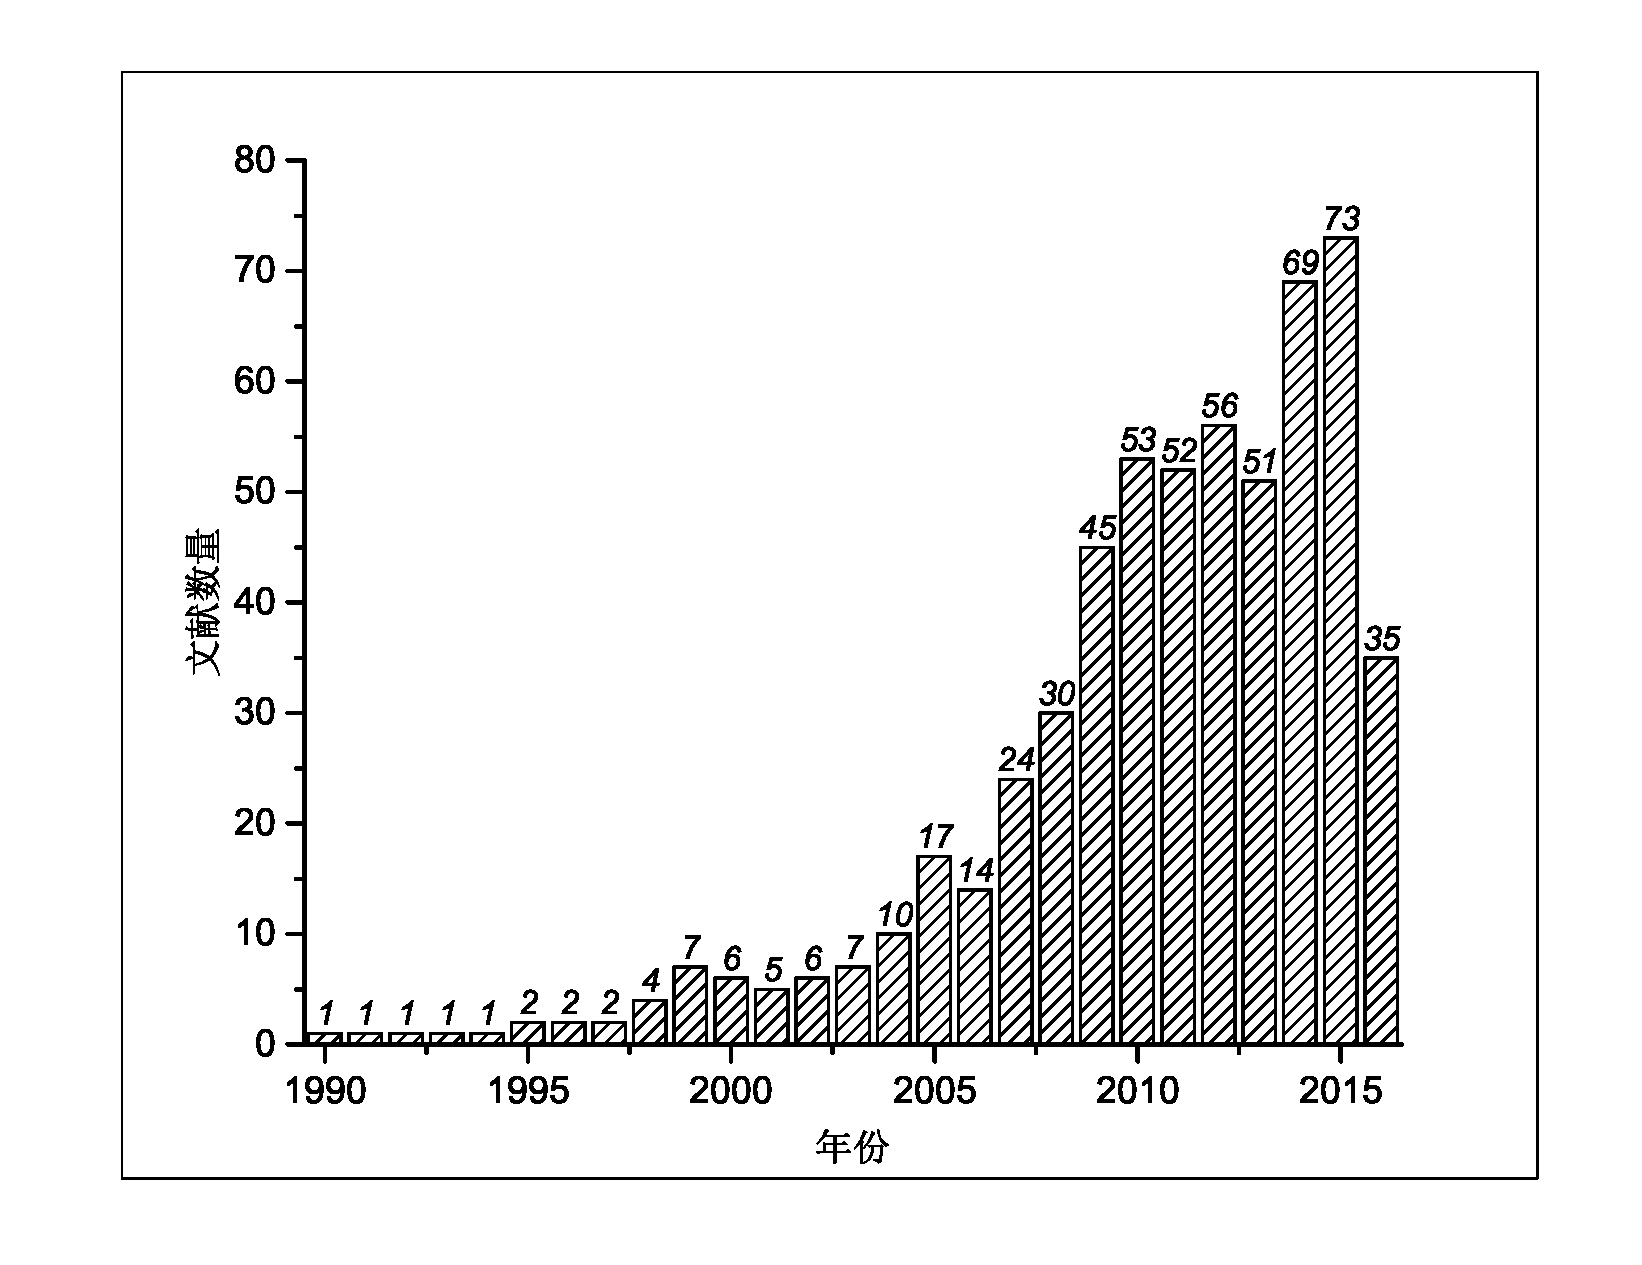
\includegraphics[width=0.8\textwidth]{literaturedistribution21}}}
%\subfigure{\label{literaturedistribution22}}\addtocounter{subfigure}{-2}
%\subfigure[Each clone number of events annually published literature]{\subfigure[各个克隆活动每年发表的文献数量]{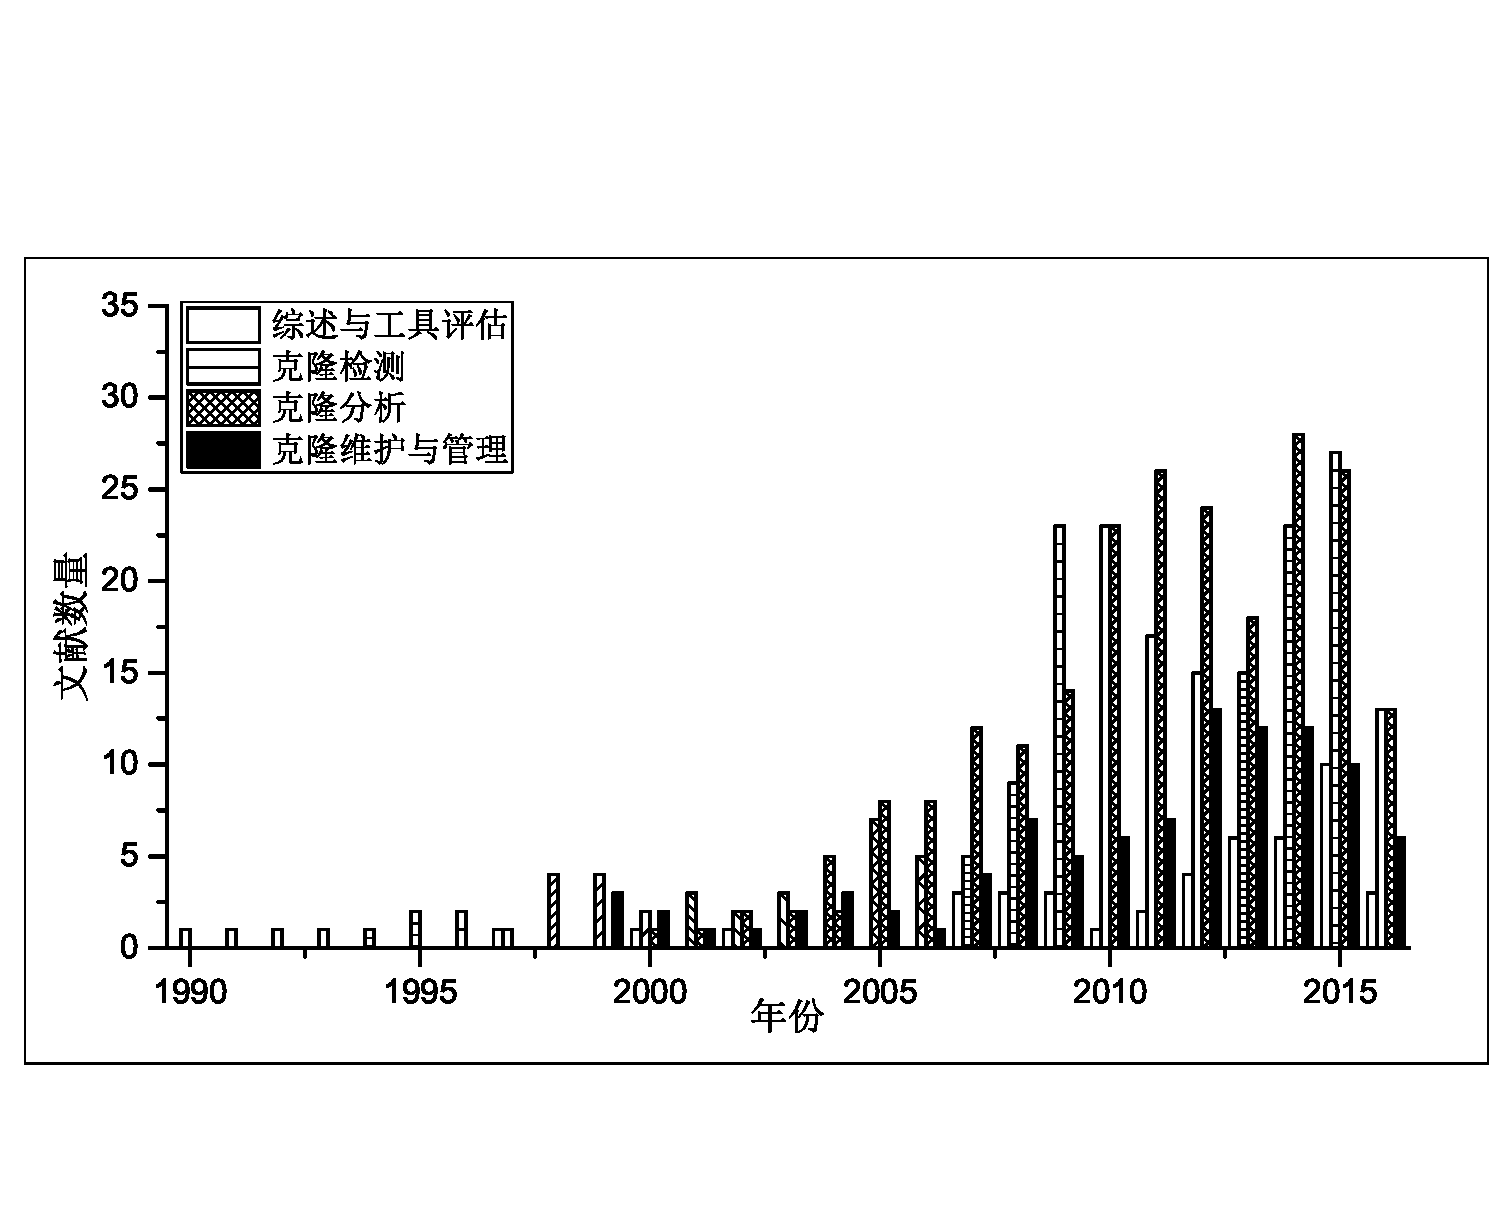
\includegraphics[width=0.8\textwidth]{literaturedistribution22}}}
%\bicaption[literaturedistribution2]{}{克隆代码领域研究趋势}{Fig.$\!$}{Cloning research trends in the code field}\vspace{-1em}
%\end{figure}

%为便于分析克隆代码研究领域的发展趋势,本文又对克隆代码研究领域的文献按照发表年份和研究方向进行了统计。统计分析结果如图~\ref{literaturedistribution2}~所示,其中图~\ref{literaturedistribution21}~是领域整体上每年发表文献数量的统计情况,图~\ref{literaturedistribution22}~是在不同研究方向上每年发表文献数量的统计情况。
%从图~\ref{literaturedistribution21}~可以看出,克隆研究可以划分为两个阶段:1990-2003年和2004-2016年。在2003年以前,克隆代码研究领域的文献数量较少,这一阶段是克隆代码研究的孕育期。而在2004年以后的近10年内,克隆代码研究领域的文献数量快速增长,并且保持在一个较高的水平上,展现出了蓬勃的发展趋势,表明此阶段是克隆代码研究的发展期。与图~\ref{literaturedistribution21}~类似,从图~\ref{literaturedistribution22}~在不同研究方向上每年发表的文献数量来看,其研究趋势也以2003年为界限划分为两个阶段。在2003年以前,克隆代码研究主要集中在克隆检测方向,处于孕育期。在2004年以后,各个研究方向的文献数量都有了快速增长,进入了发展期。其中尤以克隆检测和分析方向的发展最为迅速,发表了大量研究成果,并依然有继续增长的趋势,说明克隆检测和分析事目前研究最为充分和最为活跃的研究方向。相比之下,克隆维护和管理仅在近几年才引起人们的关注,对克隆维护和管理的研究虽然近几年才刚开始起步,文献数量占比相对较少,但已呈现出逐年增长和后来者居上的趋势,说明克隆维护和管理正在逐渐成为克隆代码研究领域的新热点。

\BiSubsection{克隆代码检测}
{Code Clone Detection }
\label{clonedetection}
克隆检测是指从软件中检测并报告克隆代码的位置的研究。相对于克隆代码研究的其他技术而言,克隆检测技术相对成熟。

\BiSubsubsection{克隆检测方法}
{Clone Detection Methods}

%%一般而言,克隆代码检测分为三个步骤:代码的中间表示、相似性匹配和报告检测结果。首先使用不同的方法对源代码进行抽象表示或转换,将其表示为抽象语法树等中间表示形式。然后对代码的中间表示形式进行相似性匹配,寻找相似的代码片段。最后报告检测结果,将彼此相似的克隆代码以克隆组的形式保存在检测结果中。
迄今为止,研究人员已提出许多种克隆检测方法,并开发了相应的检测工具。根据所使用的技术不同,可以将克隆检测划分为基于文本(Text)的方法、基于Token的方法、基于树(如Abstract Syntax Tree,AST)的方法、基于程序依赖图(Program Dependency Graph, PDG)的方法和基于度量值(Metric)的方法。

基于Text的克隆检测方法是通过直接比较源代码文本,使用字符串匹配等算法来检测克隆代码。因其并没有对源程序进行词法分析,大部分仅可以较好地支持Type 1克隆的检测。目前使用较多的基于文本的克隆检测工具主要有duploc\cite{ducasse1999language}、Simian\cite{Simian}、DuDe\cite{wettel2005archeology}、SDD\cite{lee2005sdd}、NiCad\cite{roy2008nicad}等。

基于Token的克隆检测方法是通过对源代码进行词法分析,获得源代码的Token序列,然后通过寻找Token序列中相似的子序列来检测克隆代码。因其对源代码进行了词法分析,所以可以较好地检测Type-2克隆代码的检测。但由于缺乏必要的语法和语义分析,使其无法较好地支持Type-3和Type-4克隆的检测。
目前使用较多的基于Token的克隆检测工具主要有Dup\cite{baker1995finding}、CCFinder\cite{kamiya2002ccfinder}、CP-Miner\cite{li2006cp}、iClone\cite{gode2009incremental}等。

基于Tree的克隆检测方法是将源代码表示为某种树的形式(如抽象语法树、代码解析树等),然后通过使用子树匹配算法从中寻找相似的子树来检测克隆代码。因其对源代码进行了语法分析,所以提高了克隆代码检测的准确率,尤其是可以较好地支持Type-3克隆的检测。但是由于子树匹配算法的时间复杂度高于前两种方法,因此这类算法的检测速度低于前两种方法。
目前使用较多的基于Tree的克隆检测工具有CloneDr\cite{baxter1998clone}、SimScan\cite{SimScan}、Deckard\cite{jiang2007deckard}、CloneDigger\cite{bulychev2008duplicate}等。

前三种克隆检测方法中所使用的中间表示形式较为容易实现,可使用程序静态分析方法或者编译器前端获得源代码的中间表示。大部分的克隆检测方法和检测工具属于前三种方法中的一种,可以检测系统中的大部分克隆代码。

基于PDG的克隆检测方法的主要思路是,将源代码转化成程序依赖图(包括数据依赖图和控制依赖图),然后通过寻找同构的子图来检测克隆代码。因程序依赖图表示了程序的语义信息,所以该方法可以支持语义相似的Type-4克隆代码的检测。但由于程序依赖图生成算法和图匹配算法的时间和空间复杂度极高,因而导致这类检测算法的时空开销过大,使其无法应用于大规模程序的克隆代码检测。
目前基于PDG的克隆检测工具主要有Duplix\cite{krinke2001identifying}等。

基于Metric的克隆检测方法是先将源代码转换为某种中间表示,然后在其基础上提取度量值并抽象为一个特征向量,然后通过计算特征向量的相似度来检测克隆代码。该方法的主要优点是检测速度快。但因基于度量值的方法高度依赖于度量值的提取,在对源码提取度量值的过程中会损失源码的部分语义信息,因此检测效果不够理想,使其应用受限。

此外,还有人使用结合两种或两种以上检测技术的混合方法来检测克隆代码。例如,Deckard在生成抽象语法树的基础上提取结构特征向量表示代码,然后使用聚类的方法寻找克隆代码\cite{jiang2007deckard}。CloneMiner先将源代码表示为Token形式,然后在此基础上通过使用频繁模式挖掘算法寻找相似模式来检测克隆代码\cite{basit2009data}。


\BiSubsubsection{克隆检测方法及工具评估}
{The Evaluation for Code Clone Detection Methods and Tools}

不同的克隆检测方法和检测工具各有其优缺点,分别适合检测不同类型的克隆代码,对同一类型的克隆代码的检测效果也不尽相同。如何针对具体的应用,选择合适的克隆检测方法和工具是困扰开发人员的一个问题。因此,
研究人员对主流的克隆检测方法及其检测工具进行了评估研究,以期为用户选择方法和工具提供指导性的建议\cite{bellon2007comparison}\cite{rattan2013software}\cite{roy2009comparison}\cite{svajlenko2014evaluating}。%%Bellon对6个克隆检测工具进行了评估,分别对比了查准率、查全率以及时间和空间等性能\cite{bellon2007comparison}。Rattan通过使用一种标准的系统文献综述方法,详细分析了克隆检测方面的213篇文献,并对不同的检测方法进行了评估分析,并给出了未来的研究方向\cite{rattan2013software}。此外,Roy重点分析了检测工具的使用技术和适用环境,对克隆检测工具的检测效果进行了详细的对比,对帮助用户选择和使用克隆检测工具有重要的指导意义\cite{roy2009comparison}\cite{svajlenko2014evaluating}。
本文也对目前较为主流的克隆检测工具和方法支持的克隆类型和检测效果等进行了评估,评估结果如表~\ref{detectionevaluation}~所示。其中,检测效果采用“较好”、“一般”和“较差”三种级别来评估:“较好”是指可以较好地支持该类型克隆代码;“一般”是指可以支持检测该类型克隆代码,但效果不佳;“较差”是指可以检测少部分的该类型克隆代码;对未支持的克隆类型未列出。

\begin{table}[htbp]
\bicaption[detectionevaluation]{}{主流克隆检测方法与工具评估}
{Table$\!$}{Evaluation for popular clone detection methods and tools}
\vspace{0.5em}
\centering
\wuhao
\begin{tabular}{cccc}
\toprule[1.5pt]
类型&工具或方法名&支持的克隆类型&检测效果\\
\midrule[1pt]
\multirow{5}{*}{Text} 
& Duploc\cite{ducasse1999language}&1、3&较好1,一般3\\
&Simian\cite{Simian}&1、2	&较好1,一般2\\
&DuDe\cite{wettel2005archeology}&1、3	&较好1,一般3\\
&SDD\cite{lee2005sdd}&1、3	&较好1,一般3\\
&NiCad\cite{roy2008nicad}&	1、2、3	&较好1、2、3\\
\hline
\multirow{4}{*}{Token} 
&Dup\cite{baker1995finding}&	1、2&较好1、2\\
&CCFinder\cite{kamiya2002ccfinder}&1、2&较好1、2\\
&CP-Miner\cite{li2006cp}&1、2、3&较好1、2,一般3\\
&iClone\cite{gode2009incremental}&1、2	&较好1,2\\
\hline
\multirow{4}{*}{Tree} 
&CloneDr\cite{baxter1998clone}&	1、2、3	&较好1、3,一般2\\
&SimScan\cite{SimScan}&	1、2	&较好1、2\\
&Deckard\cite{jiang2007deckard}&	1、2、3	&较好1、2,一般3\\
&CloneDigger\cite{bulychev2008duplicate}&	1、2、3	&较好1、3,一般2\\
\hline
\multirow{2}{*}{PDG} 
&Duplix\cite{krinke2001identifying}&	1、2、3、4	&较好1、2,一般3,较差4\\
&Gabel\cite{gabel2008scalable}&1、2、3、4	&较好1、2、3,一般4\\
\hline
\multirow{2}{*}{Metric} 
&Kontogiannis\cite{kontogiannis1996pattern}&	1、2、3、4	&较好1、2,较差3、4\\
&Mayrand\cite{mayrand1996experiment}&	1、2、3、4	&较好1、2,较差3、4\\
\bottomrule[1.5pt]
\end{tabular}
\end{table}

从表~\ref{clonedetection}~可以看出,基于Text的检测工具不支持Type-4克隆的检测。对Type-1克隆的检测效果最好,对Type-3克隆的检测效果一般。而对Type-2克隆支持较弱,仅有两个工具可以支持。原因是Type-2克隆是标识符重命名的克隆代码,基于Text的方法不能很好地处理标识符重命名问题。基于Token的检测工具同样不支持Type-4克隆的检测,但是可以较好地检测Type-1和Type-2克隆。支持Type-2克隆检测的原因是在将源程序转换成Token序列时进行了词法分析,因此可以解决标识符重命名的问题。但仅有一个工具可以检测Type-3克隆代码,并且检测效果一般。基于Tree的检测工具,同样不支持Type-4克隆的检测,但是对Type-1克隆的检测效果较好,并且几乎都支持Type-2和Type-3克隆的检测。由于采用的匹配算法不同,对Type-3即近似克隆的检测效果不尽相同,有些可以较好地支持Type-2克隆的检测,有些则较好地支持Type 3克隆的检测。基于PDG的检测方法不仅可以较好地检测Type-1和Type-2克隆,还可以以不同的程度支持Type-3和Type-4克隆的检测。但因其复杂度相对较高,使其并没有太多的检测工具可以利用。基于Metric的检测方法目前仅有一些检测方法被提出\cite{kontogiannis1996pattern}\cite{mayrand1996experiment},缺少相应的检测工具。

%可见,目前克隆检测方法对Type-1和Type-2克隆的检测最简单,因此效果最好,检测工具也最多;对Type-3克隆的检测相对于前两种有一定的难度,因此效果一般,但也有少量工具支持;对Type-4克隆的检测难度最大,因此效果最差,工具最少。此外,基于Text、基于Token、基于Tree的克隆检测方法实现容易,是目前较为主流的方法,相应的检测工具也较多。基于PDG的克隆检测方法受到图匹配算法复杂性的影响使得这类方法的实现难度较大,因此实用工具不多。而基于Metric的克隆检测因为检测效果不够理想,所以研究较少,也没有可用的检测工具。其次,目前绝大多数的克隆检测工具仅支持单版本的克隆代码检测,无法同时检测多个版本中的克隆代码。少数的克隆检测工具(如iClone)采用了增量式的克隆代码检测方法,即在旧版本克隆检测的基础上对新版本进行克隆代码检测,从而节约了检测时间,提高了检测效率。此外,目前绝大部分的克隆检测工具也没有集成到软件开发环境中,开发人员无法在开发过程中实时地检测和跟踪克隆代码。因此,研究如何提高Type-3和Type-4克隆的检测效果,以及如何在软件开发过程中增量式地检测克隆代码,这既是一个难点问题,也是未来的一个研究重点问题。

\BiSubsection{克隆代码分析}
{Code Clone Analysis}

克隆分析是指使用各种技术手段分析系统中的克隆代码,并挖掘其隐含的特征,旨在帮助软件开发人员更好地理解和维护克隆代码。目前的克隆分析研究主要集中在克隆演化分析、克隆评价分析上。

\BiSubsubsection{克隆代码演化}
{Code Clone Evolution}

%克隆代码往往存在于软件系统的多个版本中,并随着软件系统进行演化。
克隆代码演化分析就是通过分析克隆代码的演化过程,提取克隆代码的演化特征,识别克隆代码的演化规律,从而辅助人们更好地理解和维护克隆代码。克隆演化研究包括克隆演化过程分析和演化特征分析两个方面。演化过程分析即模型化克隆代码的演化过程。演化特征分析是分析克隆代码在演化过程中表现出来的演化特征或演化模式及其对软件质量的影响。

克隆演化过程分析最早是2001年由Antoniol等人提出的,使用时间序列描述克隆代码的演化模型\cite{antoniol2001modeling},但并未引起人们的重视。2005年,Kim提出了克隆家系模型用于描述克隆代码的演化过程,被认为是迄今为止最好的演化模型\cite{kim2005empirical}。Roy使用函数映射帮助构建克隆家系,并开发了gCad克隆家系提取器,大大提升了构建克隆家系的时间效率\cite{saha2011automatic}。Bakota通过映射不同版本的克隆来分析克隆代码的演化过程,并使用克隆坏味(Clone Smell)帮助分析克隆代码对系统的影响\cite{bakota2011tracking}。Harder对现有的演化模型进行分析\cite{harder2009modeling},指出通过分析克隆演化特征可以帮助程序开发和维护人员理解和维护克隆代码。

究竟哪些演化特征能真实准确地反映克隆代码的规律?这是克隆演化分析的难点问题。因此目前对克隆演化分析的研究主要集中在研究确定提取克隆代码的哪些特征作为演化特征以及如何提取这些特征。目前,常用的克隆演化特征主要包括克隆寿命、克隆稳定性与一致性变化。

%克隆寿命是指克隆代码在系统中的存在时间。Kim研究发现克隆代码要比非克隆代码更加稳定,同时寿命也更长\cite{kim2005empirical};进一步对长寿命的克隆代码进行研究后,发现对克隆代码的修改会使得克隆代码的寿命变短\cite{cai2011empirical}。Krinke通过对比克隆和非克隆代码,也发现克隆代码比非克隆代码的寿命更长\cite{krinke2011cloned}。通过对精确克隆和近似克隆的演化分析,发现其在演化过程中所表现出来的共同特点是:尽管克隆代码比率会随着时间而逐渐降低,但克隆代码的存在时间往往都会超过一年\cite{bazrafshan2012evolution}。因此,克隆代码会长时间的存在于系统中,在其生存期间克隆代码往往会发生变化,其变化规律与具体的软件系统相关\cite{gode2009evolution}。

%克隆稳定性关注的是在克隆代码的生存期内是否发生变化。被研究者普遍认可的观点是寿命较长的克隆代码是稳定的\cite{krinke2008cloned}\cite{gode2011clone}\cite{harder2013cloned},不会对系统造成不利的影响,也不会增加系统的维护成本。但是在克隆代码是否比非克隆代码更稳定这个问题上还存在一定的分歧。例如Gode研究发现大部分克隆是稳定的,不会发生变化\cite{gode2011frequency}。而Rahman的研究却发现克隆代码比非克隆代码更容易发生变化,是不稳定的\cite{rahman2014change}。Mondal给出了更为细致的分析结果,即Type-1、Type-2克隆是不稳定的,Type-3克隆是稳定的;并且发现克隆代码比非克隆代码的变化更分散,Type-3克隆比Type-1和Type-2克隆的变化更分散\cite{mondal2012comparative}\cite{mondal2012dispersion}。%%由此可见,在克隆代码的稳定性特征方面尚未达成共识,仍需要进一步研究。

%克隆代码的变化包括一致性变化和不一致性变化。遗忘一致性变化将会引发相关的软件缺陷,因此一致性变化也是克隆演化分析研究中需要关注的特征。Gode的研究发现发生一致性变化的克隆代码占克隆代码的比例很小\cite{gode2011frequency}。Krinke的研究进一步发现发生一致性变化和不一致性变化的克隆代码比例大约各占一半,并且大部分发生不一致性变化的克隆代码在后续的演化过程中不会继续发生变化\cite{krinke2007study}。Mondal等人的研究发现发生一致性变化的克隆代码可能会导致延迟传播现象。延迟传播是指某一个克隆片段的变化没有立即传播到其所在的克隆组中,而在间隔一定数量的版本后传播,继续发生一致性变化。研究表明延迟传播在Type-3的克隆中出现的更为频繁,软件开发人员应该重点关注Type-3克隆代码的变化,以避免引入克隆代码相关的软件缺陷\cite{mondal2016comparative}。

表~\ref{characteristic}~列出了目前对克隆演化特征的研究情况。由表中可以看出,研究者较为关注的克隆演化特征是克隆寿命、克隆稳定性与一致性变化。上述三个特征并不是相互独立的,克隆寿命会受到稳定性和克隆变化的影响,同时克隆稳定性与克隆变化之间存在对立关系。对克隆演化分析的研究大多属于实证研究,往往会较多地依赖于具体被用于实验分析的软件系统,这就导致了不同的研究可能得出不同的结论。例如对克隆稳定性的研究就出现了截然相反的观点。尽管如此,克隆演化特征分析依然可以给开发人员提供有价值的建议。一个普遍的共识是在维护和管理克隆代码的过程中更应关注那些克隆寿命较短、稳定性较差、发生一致性变化的克隆代码。%%但克隆寿命、克隆稳定性和一致性变化之间究竟存在着怎样的关系,它们对软件质量究竟会产生怎样的影响,还有哪些影响软件质量的克隆代码特征,还有待进一步深入的研究。

\begin{table}[htbp]
\centering
\bicaption[characteristic]{}{克隆演化特征分析}
{Table$\!$}{The analysis of clone evolutionary characteristic}
\vspace{0.5em}
\wuhao
\begin{tabularx}{0.9\textwidth}{llX}
\toprule[1.5pt]
文献&克隆模式、特征&结论\\
\midrule[1pt]
\cite{kim2005empirical}&	克隆寿命/一致性变化	&观察并分析克隆家系寿命与一致性变化规律\\
\cite{cai2011empirical}&	克隆寿命&	克隆寿命与克隆修改次数、新增和减少有关\\
\cite{krinke2011cloned}&	克隆寿命&	克隆代码的寿命比非克隆的寿命更长\\
\cite{bazrafshan2012evolution}\cite{gode2009evolution}&	克隆比率/寿命/变化规律	&克隆比率会随时间降低,会存在超过一年,存在期间变化规律往往和具体系统相关\\
\hline
\cite{krinke2008cloned}&克隆稳定性&	克隆代码比非克隆代码更稳定\\
\cite{gode2011clone}\cite{harder2013cloned}&	克隆稳定性&	克隆代码十分的稳定\\
\cite{gode2011frequency}&	克隆变化/一致性变化&	大部分克隆不会变化,一致性变化会更少\\
\cite{rahman2014change}&	克隆稳定性&	克隆会比非克隆更容易发生变化\\
\cite{mondal2012comparative}\cite{mondal2012dispersion}&	克隆稳定性/变化分布&	Type-1、Type-2是不稳定的,Type-3是稳定的;发现克隆代码变化比非克隆更加分散,同时Type-3克隆比Type-1和Type-2更加分散\\
\hline
\cite{krinke2007study}&	一致性变化&	一半的变化是不一致变化,且发生不一致性变化后,在后续的时间内会保持这种变化\\
\cite{mondal2016comparative}&	延后传播&	Type-3更容易发生延后传播并导致缺陷\\
\bottomrule[1.5pt]
\end{tabularx}
\end{table}


\BiSubsubsection{克隆代码评价}
{Code Clone Evaluation}

克隆评价分析主要是分析克隆代码对系统产生的影响,以便辅助开发人员更好地理解和维护克隆代码。克隆代码是否有害一直是克隆评价关注的一个热点,也是争论的一个焦点问题。因此,克隆评价研究主要是围绕着克隆代码是否有害而展开的,只是在不同阶段,人们对克隆代码的态度有所不同,研究的关注点也因此有所不同而已。

在研究的初始阶段,人们大多倾向于认为克隆代码都是有害的,因而研究的侧重点是克隆代码是否会引发软件缺陷(即克隆代码相关的缺陷分析),以及克隆代码是否会增大系统的维护代价(即克隆代码的维护代价分析)。然而随着对克隆代码研究的深入,人们研究发现虽然克隆代码有时会对软件质量产生一些负面影响,但并不一定都是有害的,从而引发了对克隆代码有害性的讨论(即克隆代码的有害性分析)。因此,克隆评价主要包括克隆相关的缺陷分析、克隆维护代价分析、克隆有害性分析等。

%在早期,有人认为克隆代码是一种最刺鼻的代码坏味,是因为它有可能会引发相关缺陷。因此,人们研究的关注点主要集中在克隆代码的缺陷分析上。例如,Juergens等人研究发现克隆代码的不一致性变化会引发相应的软件缺陷,从而降低了软件质量\cite{juergens2009code}。Gauthier通过对克隆代码进行安全性分析,在开源软件Joomla和Moodle中发现了几个潜在的影响软件质量的安全漏洞和缺陷\cite{gauthier2013uncovering}。但也有另外一些证据表明克隆代码的不一致性变化并不一定会引发缺陷,因此不会对软件质量产生显著的影响。例如,Bettenburg对不一致性变化是否引发缺陷的研究发现,仅有极少数的不一致性变化会引发缺陷\cite{bettenburg2009empirical}。文献\cite{wagner2016relationship}的研究则表明Type 3克隆代码中大约有17\%的代码含有缺陷,并且Type 3克隆不容易发生不一致性变化。文献\cite{elish2015fault}通过对缺陷密度的分析发现,面向对象程序中的克隆类含有更少的缺陷,并且Type 3克隆含有的缺陷最少。因此有人将克隆代码研究应用到缺陷检测中,但没有直接证据证明克隆代码与缺陷密切相关\cite{lo2012active}\cite{kamei2011empirical}。%%因此,克隆缺陷分析并不能直接证明克隆代码是有害的。

%除了克隆相关的缺陷分析外,还可以从维护代价的角度去分析克隆代码对软件产生的影响。Harder通过实验发现克隆代码的存在并不会增加缺陷修复的时间,但是缺陷未被修复则可能导致维护代价的增加\cite{harder2012controlled}。Lozano通过研究克隆代码的可变性,也发现克隆代码的存在会增加软件维护的代价\cite{lozano2008assessing}。Juergens不仅认为克隆代码会增加维护代价,还提出了一个计算模型来计算克隆维护代价\cite{juergens2010much}。而Monden的研究则发现包含少量克隆代码的软件模块比不含克隆代码的软件模块更可靠,但含有大量克隆代码的软件模块则正相反,实验表明克隆代码与软件可靠性和维护代价有一定的关联,但这种关联关系并不十分明确\cite{monden2002software}。以上维护代价分析的研究表明克隆代码的存在有可能会增加软件的维护代价,但是如何定量地计算克隆代码引起的维护代价仍然是一个尚未解决的问题。

%%虽然缺陷分析和维护代价分析可用于评价克隆代码对软件产生的影响,但却不能作为评价克隆代码是否有害的直观证据。正因如此,近些年来,研究人员又展开了克隆代码有害性分析的研究。Kapser通过对比11种克隆模式在软件开发和维护过程中的优缺点,并在开源软件Apache和Gnumeric上进行实证研究,发现在Apache中大约有71\%的克隆代码被分类为有益克隆,对系统维护具有积极的影响,是一种合理的存在方式,因此人们应当正视在开发过程中克隆代码的长期存在\cite{kapser2006cloning}\cite{kapser2008cloning}。Kapser通过对Apache Web Server中的克隆代码进行分析,研究发现其中一个子系统中聚集了大量的克隆代码;该子系统的克隆代码增加了系统的功能性,对软件开发过程是有益的\cite{kapser2006supporting}。Selim使用风险模型判定克隆代码是否有害,研究结果发现克隆代码并不比非克隆代码具有更高的有害风险\cite{selim2010studying}。Wang提出利用贝叶斯网络对克隆代码进行有害性预测的方法\cite{wang2012can},该方法可用于辅助开发人员决定是否可以通过复制粘贴的方式引入新的克隆代码。Higo则提出一种提取有问题的克隆代码(有害克隆)的方法,该方法先对程序进行标准化,然后利用检测工具检测克隆代码,最后对检测到的克隆代码进行过滤、合并等操作来提取有问题的克隆代码,在Linux内核2.6.6上的实验结果表明只有少数克隆代码是有问题的克隆代码\cite{higo2009problematic}。Hordijk提出了一个结构化的证据模型分析克隆代码的有害性,研究结果表明只有少部分的证据证明克隆代码是有害的,并且仍需更多的研究去支撑这一结论\cite{hordijk2009harmfulness}。%%从上述对克隆代码有害性分析的结果不难得出结论,克隆代码并非都是有害的,但是究竟具有什么特征的克隆代码是有害的,还是一个有待深入研究的问题。

表~\ref{evaluation}~对克隆评价分析研究进行了分类统计,使用“积极”、“中立”和“消极”三种评价标准对现有的克隆评价分析方法进行了总结。“积极”是指克隆代码的存在对系统有积极的影响;“中立”是指克隆代码不会对系统产生影响;“消极”是指克隆代码会对系统产生消极的影响。从表中可以看出,大部分研究对克隆代码持积极和中立的态度,仅有少数持消极态度。这从另外一个侧面表明目前对克隆代码是否有害还存在一定的分歧,主要原因是对克隆代码缺少统一的评价标准以及深入的特征挖掘与分析。%%,当然这也是克隆评价分析中的最具挑战性的问题。

\begin{table}[htbp]
\centering
\bicaption[evaluation]{}{克隆评价分析}{Table$\!$}{The analysis of clone evaluation}\vspace{0.5em}\wuhao
\begin{tabularx}{0.9\textwidth}{lllX}
\toprule[1.5pt]
&文献&评价&结论\\
\midrule[1pt]
\multirow{6}{*}{\rotatebox{270}{克隆缺陷分析}} 
&\cite{juergens2009code}&消极&研究发现不一致变化在克隆中发生较为频繁,同时也会导致相应的缺陷\\
&\cite{gauthier2013uncovering}&消极&通过对不安全的克隆代码分析,发现了几个安全漏洞和缺陷\\
&\cite{bettenburg2009empirical}&积极&克隆代码的不一致变化并不会引入缺陷,不会对软件的质量产生影响\\
&\cite{elish2015fault}&积极&克隆代码含有更少的缺陷,Type 3所含有的缺陷最少\\
&\cite{lo2012active}&中立&克隆代码研究应用到缺陷检测中,但没有直接证据证明与缺陷相关\\
&\cite{kamei2011empirical}&中立	&通过实验发现并不会增加缺陷修复时间,但是缺陷未被修复,可能会产生维护代价的增加\\
\midrule[1pt]
\multirow{4}{*}{\rotatebox{270}{克隆维护代价分析}} 
&\cite{wagner2016relationship}&中立	&Type 3克隆中有17\%含有缺陷,并且Type3克隆更容易发生一致性变化\\
&\cite{harder2012controlled}&消极&通过对克隆代码的可变性研究发现克隆代码确实会增加其方法可变化的维护代价,但没有确切的证明会说明克隆会增加系统维护代价\\
&\cite{juergens2010much}&消极&认为克隆会增加维护代价,并且提出了一个代价计算模型计算这次代价\\
&\cite{monden2002software}&中立&Monden却发现包含克隆的模块比不含克隆的模块更可靠,同时含有大量克隆的模块却相反实验表明了克隆与系统可靠性和维护代价的关系,但是这种关系仍然不够明朗\\
\midrule[1pt]
\multirow{6}{*}{\rotatebox{270}{克隆有害性分析}} 
&\cite{selim2010studying}&积极&克隆代码并不比非克隆代码具有更高的有害风险\\
&\cite{kapser2006cloning}\cite{kapser2008cloning}&积极	&发现最多有71\%的克隆对系统的可维护性具有积极的影响\\
&\cite{rahman2012clones}&积极	&克隆并不是真正的代码坏味,克隆是无害的\\
&\cite{wang2012can}&中立	&预测克隆有害性,其中有害的较少,无害的较多\\
&\cite{higo2009problematic}&中立&使用分类模型抽取有问题的克隆代码,只有少部分是有问题的克隆\\
&\cite{hordijk2009harmfulness}&中立&现有研究不能支撑克隆有害的观点,仍需进一步的研究\\
\bottomrule[1.5pt]
\end{tabularx}
\end{table}

\BiSubsection{克隆代码维护}
{Code Clone Maintenance}

克隆维护是解决克隆代码问题的直接途径,主动地解决克隆代码可能或已经引发的问题。克隆维护与软件开发过程结合得较为紧密,维护的方法主要包括克隆重构、克隆规避、克隆复用和克隆管理。

\BiSubsubsection{克隆代码重构}
{Code Clone Refactoring}

重构作为一种常见的软件维护手段,是指在不改变软件外部行为的条件下改变软件的既有设计\cite{kerievsky2006重构与模式}。重构应用于克隆维护中,指的是通过重构手段消除系统中的克隆代码。

由于重构所需的条件较为苛刻,同时重构的代价也较大,还需考虑重构安全的问题。因此,在重构前对克隆代码进行可重构性分析和重构排序显得尤为重要。可重构性分析旨在识别适于重构的克隆代码候选集合,以提高克隆重构的效率。Lin等人通过对克隆代码进行差异性分析,帮助开发人员决定是否进行重构操作和如何执行重构操作\cite{lin2014detecting}。Mende实现了一个工具支持可重构性分析,在软件中识别可以被重构的函数克隆\cite{mende2009evaluation};Schulze提出了一个用于识别可重构的克隆代码的克隆分类方法,通过计算克隆代码的可重构指数识别可重构的克隆代码\cite{schulze2008towards};Choi等人提出了基于度量值的可重构性分析方法,可以快速地识别可重构的克隆代码\cite{choi2011extracting}。识别可重构克隆后,为了节省重构时间,还可以对克隆代码进行重构排序或者调度。如Mandal先通过分析克隆演化模式来确定克隆候选,然后使用关联规则挖掘进行可重构排序、\cite{mandal2014automatic};Lee采用遗传算法对重构进行调度,以确定重构顺序帮助改进软件质量\cite{lee2011automated};Zibran提出一种极限编程方法对克隆代码进行重构调度\cite{zibran2011constraint}。另外,Liu等人提出了一个重构调度方法帮助优化调度过程\cite{liu2012schedule}。尽管该方法不是针对克隆重构的,但也可以考虑将其应用于克隆代码的重构调度上。此外,Radhika等人仅考虑重构代价对所有的克隆代码进行重构排序,未考虑克隆代码是否适合重构的问题\cite{venkatasubramanyam2013prioritizing},应该结合可重构性分析指导克隆重构。
克隆重构最主要的目的是消除系统中的克隆代码。Higo等人开发了一个工具ARIES,根据克隆代码的结构信息识别可重构的克隆代码,然后通过计算不同的度量值来确定使用哪一种目前已有的重构方法移除克隆代码\cite{higo2008metric}。Krishnan通过分析克隆代码的程序依赖图,确定给定克隆代码能否被安全的重构,然后通过检测和参数化克隆代码的差异点对克隆代码进行重构,取得了较好的效果\cite{krishnan2014unification}。Barbosa使用四种规则重构克隆代码,并在开源软件JhotDraw上进行了实验,结果表明基于规则的重构方法可以有效地移除软件中的克隆代码\cite{barbosa2013removing}。

在重构完成后,对重构后代码进行分析,还可以得出一些结论以进一步指导克隆重构。G{\"o}de通过对维护人员使用的重构方法和被重构的克隆代码进行实证研究,发现在不同的软件系统中都存在克隆重构的行为,并且克隆重构不是经常性地发生而是有选择性地发生\cite{gode2010clone}。Zibran等人通过克隆重构研究,回答了所提出的关于克隆重构的七个研究问题,并且研究发现克隆规模对克隆重构没有重要的影响,同时在软件早期的版本中重构会较为频繁地发生,发生重构的克隆在重构前往往是较为稳定的克隆代码\cite{zibran2013evaluating}。Choi通过对重构行为进行观测,识别出几种较为频繁的克隆重构模式,并且分析了每种重构模式的特征,这些都有助于进一步指导克隆代码的重构\cite{eunjong2014investigation}。Tairas通过对克隆代码的重构性分析,提出了子克隆的概念,并研究发现子克隆的重构行为更容易发生,因此建议在对克隆代码的维护过程中应重点考虑子克隆的重构\cite{tairas2010sub}。

%%目前,虽然已有重构方法以插件的形式集成到了eclipse中 ,支持在软件开发过程对一般代码坏味重构。由于一般代码坏味的重构方法不一定适合克隆代重构,所以尚未有在软件开发环境中针对克隆代码的重构方法。此外,重构是在克隆代码出现后用以消除克隆代码的一种被动的软件维护方法,而且并非所有的克隆代码都适合重构。因此重构不是解决克隆代码维护难题的最有效的方法,更有效的方法是在软件开发过程中主动地规避或维护克隆代码,这是克隆维护中的一个难点问题。

\BiSubsubsection{克隆代码规避}
{Code Clone Prevention}

克隆规避也称克隆预防,是在克隆产生时通过某种策略或手段进行干预,以避免克隆代码的产生。克隆规避是一种预防性的克隆维护方法,通过阻止克隆代码产生来降低克隆维护的代价。

软件开发人员的复制粘贴活动是导致克隆代码产生的最主要原因。因此在复制粘贴时对新产生的克隆代码进行分析,帮助软件开发人员决定是否规避克隆代码,是目前常见的克隆规避方法。Ali曾提出一个克隆规避的概念模型\cite{ali2013enhancing},尽管对克隆规避研究具有一定的指导意义,但并未给出该模型的具体实现方法。Wang等人基于贝叶斯网络在复制粘贴时预测克隆代码的一致性变化,通过判断一致性变化决定是否规避该新产生的克隆代码\cite{wang2012can}\cite{wang2014predicting}。Ravikanth通过分析复制粘贴操作的前置和后置条件,来确定是否允许对被复制的克隆代码实施粘贴操作,从而实现克隆规避\cite{venkatasubramanyam2012method}。

%%由于受软件复用的影响和编程语言的限制,大部分克隆代码是无法避免的。克隆规避可以作为一种辅助的手段通过限制开发人员在软件开发过程中的复制粘贴操作帮助减少克隆代码的产生,但却无法规避全部的克隆代码。在实际的应用中,还需要将克隆规避和克隆管理相结合,对可以规避的克隆代码采用规避技术进行主动地规避,对无法规避或者无需规避的克隆代码采用跟踪的方式进行管理,以主动地维护这些代码。

\BiSubsubsection{克隆代码复用}
{Code Clone Reuse}

在软件开发过程中,复用既有代码是一种常见的软件开发手段。近些年来,随着对克隆代码评价分析研究的深入,人们已经意识到复用健壮性好的克隆代码不仅有助于缩短软件开发周期,还有利于提高软件的健壮性和可维护性。%%因此,对克隆复用的研究在近些年来引起了人们的关注,成为克隆代码领域中的一个新的研究方向。不过,相对于克隆检测和分析而言,目前对克隆复用的研究还相对较少。

Krutz等人提出克隆数据库概念,将已有克隆代码组织为克隆数据库,并结合代码检索技术实现对克隆代码的复用\cite{krutz2014code}。Ishihara提出的方法也允许开发人员通过代码搜索技术搜索可以复用的克隆代码\cite{ishihara2013reusing}。Ohta通过对比软件开发过程中由复制粘贴操作产生的克隆代码和系统中已存在的克隆代码,并将该克隆代码划分为较差、较好、最好三种情况,辅助开发人员决定是否能够复用该克隆代码\cite{ohta2015source}。但该方法对克隆代码的可复用性评价仅依赖于开发人员的复制粘贴操作,仅在复制粘贴操作发生后给出可复用性建议,无法在复制粘贴操作发生前为开发人员提供可复用的克隆代码信息。在软件开发过程中直接向开发人员提供一个已经通过某种评价方式确定是否可复用的克隆代码库,是一种更为主动的克隆代码复用形式。例如,Yang\cite{yang2015classification}等人使用机器学习模型对克隆代码进行分类,分类标准由开发人员动态地标记,通过标记可复用的克隆代码将该方法应用于克隆复用,辅助开发人员搜索可以复用的克隆代码。Ohtani从代码建议的视角辅助开发人员复用已有的代码,从不同粒度(关键字级别、方法级别和混合方法)对可复用的代码提供搜索支持,实验结果表明混合方法可以更精确地提供代码是否可复用的建议\cite{ohtani2015level}。Kintab实现了一个克隆代码的专家推荐系统,可以在线向软件开发人员提供复用克隆代码的相关咨询,软件开发人员可以根据专家的建议决定如何复用和维护既有的克隆代码\cite{kintab2014recommending}。

%%软件复用在提高软件开发效率的同时,势必也导致产生大量的克隆代码,这就使得克隆复用研究面临着一些新的问题。例如,如何实时地跟踪、维护和管理一个可复用的克隆代码库,在保证软件开发质量的前提下,主动地复用既有代码,以提高软件开发效率,既是一个新问题,也是一个难点问题。

现有的克隆代码复用研究大都是针对单一项目的。如何实现对跨项目的克隆代码复用是克隆复用面临的另一个新问题。目前,在互联网环境下,大量的开源社区里也普遍存在代码复用的情况,由此产生了跨项目的克隆代码和对跨项目代码复用的应用需求。但目前对这种跨项目的克隆代码复用的研究依然较少。Ishihara对跨项目的软件进行函数克隆检测,试图建立一个公用函数库用于代码复用\cite{ishihara2012inter}。Cheng等人研究了跨项目的克隆代码检测技术\cite{cheng2016feasibility}。Tairas等人将信息检索技术与克隆代码分析相结合,以便快速有效地搜索可复用的克隆代码\cite{tairas2009information}。事实上,以上这些技术都可以用于跨项目的克隆代码搜索和复用中。

\BiSubsubsection{克隆代码管理}
{Code Clone Management}

%%克隆代码的重构是在克隆代码产生之后消除克隆代码及其对系统产生的影响,这种维护方式属于一种较为被动的维护方式,其维护代价本来就较高。而克隆代码往往又会随时间的推移和需求的变更而在软件系统中发生变化或者产生新的克隆代码,频繁地重构势必进一步增大克隆代码维护的代价。如果将克隆代码的维护提前到软件开发阶段,在软件开发过程中跟踪克隆代码的变化,并主动地规避克隆代码的产生,则势必会降低后期维护的代价。而若要实现这种主动的维护方式,则需要从克隆代码管理的角度解决克隆代码的维护难题,即通过在软件开发过程中实现边开发、边管理克隆代码,以主动的方式维护克隆代码,消除克隆代码对软件系统的不利影响。

克隆代码管理(简称克隆管理)的概念最早是1997年由Koschke提出的\cite{koschke2008frontiers},但当时并未引起人们的重视。随着克隆代码规模的逐渐增大,人们发现现有手段无法有效解决克隆代码维护难的问题时,才开始把目光重新转向对克隆管理的研究。目前克隆管理被认为是解决克隆代码维护难题的最有效的方式。早在2012年的面向工业界的克隆管理会议\footnote{Software Clone Management Towards Industrial Application}中,就有专家学者指出克隆管理是未来的重要研究方向,如何将克隆管理与软件开发过程相结合并使之适用于工业界是目前克隆研究领域急需解决的问题\cite{koschke2012software}。%%但是目前人们对克隆管理的研究仍处于起步和理论研究阶段,罕有从管理的角度维护克隆代码的研究报道。

%Koschke将克隆管理划分为预防性、补偿性和改正性三种类型\cite{koschke2008frontiers}。预防性克隆管理的目标是避免克隆代码,关注于避免新的克隆代码的产生,而不是对已有克隆代码的管理。补偿性克隆管理的目标是发现克隆代码所引发的问题,并对其对系统造成的不利影响进行补偿。改正性克隆管理的目标是以主动的方式消除可能对系统产生不利影响的克隆代码。然而,Koschke对克隆管理的这种划分方法的理论意义大于实际意义。目前克隆管理研究主要集中于补偿性克隆管理,而改正性克隆管理尚未具体应用到实际的克隆管理中。

%Roy在文献\cite{roy2014vision}中对克隆管理研究进行了详尽的阐述,指出目前对克隆管理的研究依然较少,尚缺少有效的克隆管理方法,尤其是对Type 3和Type 4克隆代码进行管理的研究还不够充分,未来应针对这两种类型的克隆代码的管理进行深入研究。尽管Roy对克隆管理的分析涵盖了克隆代码领域的大多数研究内容,但只是以工作流的形式组织这些研究内容,并未考虑这些研究内容之间的联系,彼此之间的信息是相互割裂的,同时也没有结合软件开发过程分析对克隆管理的要求,更没有给出具体的克隆管理方法。

克隆代码管理的主要目的是降低克隆代码维护的代价。目前克隆管理的研究内容主要包括克隆跟踪、克隆变化管理以及克隆管理工具。其中,克隆跟踪是研究跟踪克隆代码产生和变化的方法。克隆变化管理是研究对克隆代码的变化进行管理的方法。克隆管理工具是研究开发有效管理克隆代码的工具。

克隆管理需要解决的首要问题是如何实时地跟踪系统中的克隆代码,包括克隆代码的产生及其变化。由于复制粘贴操作是导致克隆产生的主要原因,因此对克隆跟踪的研究主要是通过监测程序员的复制粘贴操作来实现的。例如,许多克隆跟踪工具CLONEBOARD\cite{de2009managing}、CnP\cite{hou2009cnp}、CPC\cite{weckerle2008cpc}、CReN\cite{jablonski2007cren}、CSeR\cite{jacob2010actively}等都是在软件集成开发环境中跟踪克隆代码的产生,但并非都能跟踪克隆代码的变化。另一方面,在软件开发过程中克隆代码可能随时发生变化,因此要实现对克隆代码的管理,不仅要跟踪克隆代码的产生,还要跟踪克隆代码的变化。Duala使用克隆区域描述符描述生成克隆代码的上下文信息,然后根据这些上下文信息实时跟踪克隆代码的变化\cite{duala2008clonetracker}\cite{duala2010clone}。该方法仅通过实验验证可以跟踪克隆代码的变化,但是并没有实现可用的插件集成到集成开发环境中,以实现对克隆代码的边开发、边管理。

跟踪克隆代码的目的是为了对克隆代码进行维护和管理。为了实现边开发、边管理克隆代码,还要对克隆代码的变化进行维护和管理。Yamanaka等人\cite{yamanaka2013applying}将克隆变化与事件通知机制相结合,将每一个克隆变化都看成一个事件,在克隆发生变化时提醒开发人员及时地对克隆变化进行维护。Cheng等人\cite{cheng2016rule}提出了一个基于Token的克隆代码一致性维护方法,当克隆组内的一个代码发生变化时,能够同时修改组内的其他克隆代码,保证克隆代码的一致性。该方法的前提是已知克隆变化需要一致性维护,但没有给出克隆变化是否需要一致性维护的判定方法。因此,Zhang等人\cite{zhang2016predicting}在克隆代码发生变化时预测克隆代码一致性维护需求。该方法通过提取克隆代码的演化信息及其相关特征,在克隆代码发生变化时辅助开发人员确定克隆变化是否需要一致性维护。Mondal等人通过对克隆组内的克隆代码排序,从而预测需要一致性维护的克隆代码\cite{mondal2014prediction}。此外,Murakami等人在克隆代码未发生变化时,预测克隆代码的下一次变化\cite{murakami2014predicting}。该方法通过分析历史版本中的克隆代码的变化情况,提取相关的特征进行变化预测,以便在软件开发过程中提醒开发人员对有可能发生变化的克隆代码进行维护。可见,克隆变化管理的关键不仅需要实时跟踪克隆代码的变化,更重要的是对发生变化的克隆代码进行及时的维护。

前面的研究只是针对不同的侧重点提出的克隆管理方法,却没有提供可以实际应用的克隆管理工具。鉴于此,Zhang基于事件通知机制实现了一个克隆管理工具,不仅可以监测克隆代码的产生,还可以监测克隆代码的维护过程\cite{zhang2013towards}。Nguyen实现了一种可用于管理克隆代码的eclipse插件JSync\cite{nguyen2012clone}。该插件支持在软件开发过程中对克隆代码进行克隆关系管理与一致性维护管理。这里的克隆关系管理是指在软件开发过程中检测系统中的克隆代码,并对具有克隆关系的代码进行管理。这里的一致性维护管理是指识别变化的克隆代码以及变化的克隆代码是否会导致不一致性缺陷,以便开发人员对克隆代码进行一致性维护。而另一个较早提出的eclipse插件CeDAR\cite{tairas2012increasing}。虽然没有强调是一种克隆管理工具,但事实上也具有一定的克隆管理功能。该插件将克隆检测和克隆重构融为一体,对现有克隆检测工具的克隆检测结果进行可重构性分析,寻找潜在的可重构的克隆代码,然后在软件开发过程中实现对克隆代码的重构。

%%如何将克隆代码的检测、分析和维护结合到软件开发过程中,以实现对克隆代码的边开发、边维护和边管理是克隆管理急需解决的一个难点问题。

\BiSubsection{当前研究中存在的问题分析}
{Problems in Current Research}

克隆代码研究已经成为了软件工程领域的一个热点问题,目前的克隆研究已经取得了相当丰富的研究成果,如克隆检测、克隆分析和克隆维护研究等,但目前的研究中仍然存在一些问题。

(1)克隆检测研究可以帮助程序开发人员快速的获得系统中的克隆代码,是目前研究的较为深入且广泛的一个研究活动。已经开发和提出了相当规模的克隆检测方法和工具,使用其可以快速高效地检测系统中存在的克隆代码。但是,克隆代码检测仅仅是克隆研究的初始阶段,即不能帮助软件开发人员理解克隆代码,又不能解决克隆代码对软件产生的不利影响。因此,克隆代码分析和维护研究将是解决克隆代码问题的关键内容。

(2)克隆代码分析可以辅助开发人员理解克隆代码,也是目前克隆代码研究中最为活跃的一个分支。在克隆分析的研究中,克隆代码演化研究是最为重要的研究内容,克隆评价研究往往也是在克隆代码演化的基础上进行,尤其是体现在演化过程的克隆代码变化对软件的影响上。但是,克隆演化分析研究中仍然不能令人满意。首先最重要的是,在目前的克隆代码的演化研究中,研究人员的研究往往集中到某一个具体的克隆代码的演化特征上,缺少从宏观上的对克隆代码演化特征的分析。例如,研究人员分别研究了克隆代码的克隆寿命、稳定性等某一个具体的问题。其次,克隆演化研究也往往带有较强的主观性,研究人员往往是通过分析既有的系统验证固有的结论,甚至出现了完全不同的研究结论。例如在对克隆代码稳定性的研究中,有研究者认为克隆代码是稳定的,也有研究者认为非克隆代码是稳定的。因此,如何从大量的克隆代码及其演化过程中全面且客观地识别克隆代码的演化特征是一个值得研究的问题。克隆代码的演化特征对于帮助程序开发人员理解克隆代码及其演化过程具有积极的意义,可以进一步提高软件的可理解性。


(3)克隆维护研究旨帮助程序开发人员解决或者避免克隆代码对系统产生的不利影响的问题。在克隆维护研究中研究人员进行了大量的研究,包括对克隆代码的重构、复用和管理等等。然而,目前克隆维护研也不能令人满意。%首先,克隆重构作为消除克隆手段,但由于其重构条件苛刻,仅能消除一小部分克隆代码,维护代价偏高。同时,由于多种原因无法规避全部的克隆代码,也无法解决克隆代码的维护难题。此外也缺少成熟有效的复用模型和方法。更为重要的是,
上述克隆维护研究没有聚焦到导致克隆代码难以维护的根本原因上。克隆代码难于维护的根本原因在于克隆代码在其演化过程的中的变化问题,尤其是克隆代码的一致性变化和不一致变化,及其由此所引发的克隆一致性缺陷和额外的维护代价问题。%克隆代码的一致性维护问题是影响软件质量的一个重要因素。克隆代码的一致性变化问题可能会导致新的克隆缺陷,而保持这种一致性也会导致克隆代码的维护代价变大,因此研究克隆代码的一致性维护需求预测显得尤为重要
如何避免、解决克隆代码的一致性变化问题是克隆维护研究中的一个值得研究的问题。通过预测克隆代码的一致性维护需求,可以有效的避免一致性缺陷,也可以降低克隆代码所导致的代价,并进一步帮助提高软件质量和可维护性。

%克隆维护是处理克隆代码所引发的相关问题的直接途径,其主要任务是通过采取措施维护系统中的克隆代码。克隆重构作为消除克隆手段,但由于其重构条件苛刻,仅能消除一小部分克隆代码,并且克隆重构属于一种被动的维护方式,维护代价偏高。一种较为主动的维护方式是克隆规避,即通过监测复制粘贴活动从源头上避免有害克隆代码的产生。但由于多种原因无法规避全部的克隆代码,也无法解决克隆代码的维护难题。此外,克隆复用作为一种常用的可以帮助提高软件开发效率的手段,依然缺少成熟有效的复用模型和方法。最后,克隆重构和复用往往需要克隆分析结果的支持,如克隆评价结果指导克隆重构和克隆复用,然而遗憾的是目前的克隆维护没有与克隆分析相结合。

\BiSection{研究内容与论文结构}
{Main Research Contents and Structure of This Dissertation}

\BiSubsection{研究内容}
{Main Research Contents}

针对软件中所存在的大量的克隆代码、以及克隆在其演化过程容易被程序开发人员修改而导致克隆代码的一致性维护问题,本文结合程序分析、克隆演化和度量提取,研究基于机器学习的克隆代码演化分析与一致性维护方法,可以有效的帮助程序开发人员理解克隆代码,并可以降低克隆代码的维护代价和避免克隆一致性缺陷,以达到提高软件质量、可理解性和可维护性的目的。本文的主要研究内容可以简述如下:

(1)针对演化中的克隆代码难于理解和分析的问题,研究基于聚类的克隆代码演化特征分析方法,使用克隆演化特征帮助程序开发人员程序分析和理解克隆代码。克隆代码随着软件系统的演化同时演化,在其演化过程中所表现出的特征称之为克隆演化特征,克隆演化特征对理解和维护克隆代码有极为重要的意义。本文结合机器学习方法,提取相应的度量值对克隆代码进行演化特征分析,获取相应的克隆代码演化特征,帮助理解和维护克隆代码。

(2)针对创建的克隆代码在其演化过程中的一致性变化往往会导致额外的维护代价问题,研究基于贝叶斯网络的克隆代码创建时一致性维护需求预测方法。将复制粘贴创建的克隆代码称为克隆创建实例,将其在未来演化过程中所发生的一致性变化称为克隆创建时一致性维护需求。通过提取代码属性和上下文属性表示克隆创建实例,并使用贝叶斯网络预测克隆代码创建时的一致性维护需求,可以帮助程序开发人员降低克隆代码的一致性维护代价。

%%变化时一致性预测
(3)针对克隆代码变化时遗忘克隆代码一致性变化会导致克隆一致性缺陷问题,研究基于贝叶斯网络的克隆代码变化时一致性维护需求预测方法。将克隆代码发生变化的克隆代码称为克隆变化实例,并将其未来演化过程中所发生的一致性变化称为克隆变化时一致性维护需求。通过提取代码属性、上下文属性和演化属性用于表示克隆变化实例,并使用贝叶斯网络预测克隆代码变化时一致性维护需求,可以帮助程序开发人员避免克隆代码一致性缺陷。


%%实证研究
(4)针对克隆代码一致性维护需求预测如何结合软件开发过程和其它机器学习方法的问题,研究基于不同机器学习方法的克隆代码一致性维护需求实证研究方法。将克隆代码创建和变化实例统称为克隆实例,并将其一致性维护需求统称为克隆代码一致性维护需求。将克隆代码的一致性维护预测扩展到其它五种不同的机器学习方法中,并与软件开发过程相结合实现边开发边预测克隆代码的一致性维护需求,帮助程序开发人员在软件开发过程中选择合适的机器学习模型和预测时间,从而实现边开发、边分析、边维护克隆代码,帮助提高软件的质量和可维护性。%帮助程序开发人员避免克隆代码一致性缺陷和降低克隆维护代价。%本文方法可以实现边开发、边分析、边维护克隆代码,帮助提高软件的质量和可维护性。

\BiSubsection{论文结构}
{Structure of This Dissertation}

基于机器学习的克隆代码分析与一致性维护方法,综合考虑程序分析方法、克隆代码演化、机器学习方法和属性提取方法实现对克隆代码的分析和维护。为了进一步说明本文的研究内容以及各个部分之间的关系,论文的主要研究内容及其关系示意图如图~\ref{framework1}~所示。本文主要研究四个内容,首先研究克隆代码的演化特征分析方法,获取克隆代码演化特征用于指导后续的克隆代码一致性维护研究。然后,针对克隆代码的一致性维护问题,分别在克隆代码创建时和变化时基于贝叶斯网络预测克隆代码的一致性维护需求,从而降低额外的克隆维护代价和避免克隆一致性缺陷价。最后结合软件开过程,将克隆代码一致性维护需求预测问题扩展到其它的机器学习方法中,帮助程序开发人员有效地维护克隆代码一致性,从而帮助提高软件质量和可维护性。

\begin{figure}[htbp]
\centering
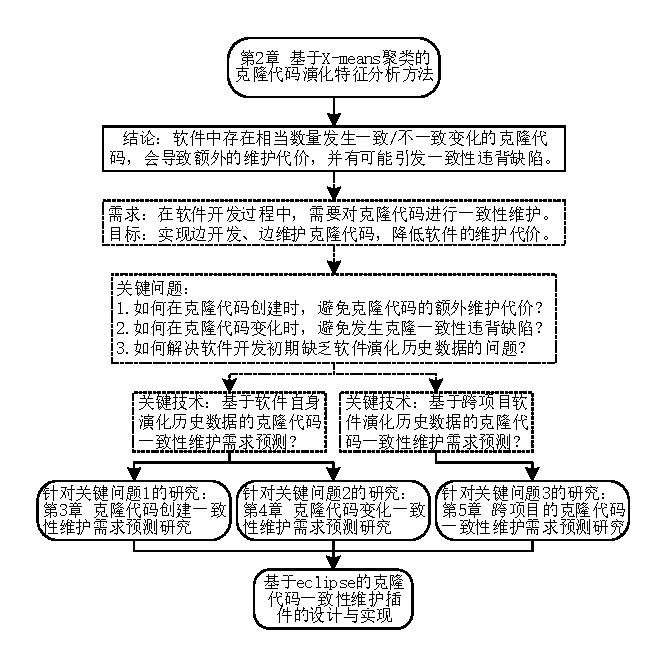
\includegraphics[width = 1.0\textwidth]{framework1.pdf}
\bicaption[framework1]{}{论文主要研究内容及其关系示意图}{Fig.$\!$}
{Main research contents and their relationship in the thesis}
%{Main Research Contents and Their Relationship in The Thesis}
\vspace{-1em}
\end{figure}

各章节研究内容安排如下:

第2章研究基于聚类的克隆代码演化特征分析方法,使用克隆演化特征帮助程序开发人员程序分析和理解克隆代码。首先,使用克隆检测工具检测系统中的克隆代码,并构建系统所有克隆代码的克隆家系用于描述克隆代码的演化过程。然后,从克隆片段、克隆组和克隆家系三个不同角度描述克隆代码及其演化过程并提取相应的度量值。最后,使用聚类分析方法聚类克隆代码并挖掘克隆代码演化特征,帮助开发人员理解克隆代码及其演化过程。

第3章研究基于贝叶斯网络的克隆代码创建时一致性维护需求预测方法,定义了克隆代码创建实例及其一致性维护需求。首先,通过检测系统的克隆代码并构建克隆家系收集系统中的克隆创建实例。然后,提取代码属性和上下文属性两组不同的度量值表示克隆创建实例的被复制和被粘贴的克隆代码。最后,使用贝叶斯网络预测克隆代码创建时一致性维护需求。

第4章研究基于贝叶斯网络的克隆代码变化时一致性维护需求预测方法,定义了克隆代码变化实例及其一致性维护需求。首先,通过检测系统的克隆代码并构建系统克隆家系收集系统中的克隆变化实例。然后,提取代码属性、上下文属性和演化属性三组不同的度量值用于表示克隆变化实例。最后,使用贝叶斯网络训练预测克隆代码变化时一致性维护需求。

第5章进行克隆代码一致性维护需求实证研究,统一了克隆代码创建和变化实例为克隆实例及其相应的克隆代码一致性维护需求。首先,检测系统的克隆代码并构建克隆家系收集所有的克隆代码实例,并使用不同的属性组表示克隆实例(与第3章和第4章相同)。然后,将克隆代码的一致性维护预测扩展到其它五种不同的机器学习方法中。最后,将克隆代码一致性维护需求预测与软件开发过程相结合,实现了一个eclipse插件可以实现边开发边预测克隆代码的一致性维护需求。

% !Mode:: "TeX:UTF-8" 

\BiChapter{基于X-means聚类的克隆代码演化特征分析}
{Analyzing Clone Evolutionary Characteristic Based on X-means Clustering}

\BiSection{引言}
{Introduction}

研究表明,软件中存在大量的克隆代码,即彼此相似的代码片段。同时,在软件随着时间进行演化的过程中,软件系统中的克隆代码并不是静止不变的。克隆代码会随着软件系统进行演化,研究人员将克隆代码的这一现象称为克隆代码演化。在克隆代码的演化过程中,在大量克隆代码及其演化过程中,必然存在着一些隐含的信息可以揭示克隆演化规律,本文将之称为克隆代码演化特征。克隆演化特征不仅可以帮助软件开发人员理解系统中存在的克隆代码,还可以向软件开发人员提供一些如何维护克隆代码的建议。但遗憾的是,当前研究中对克隆演化特征的研究不够充分,缺乏客观且全面的克隆演化特征分析方法。因此,如何分析并获取克隆代码演化特征是一个值得研究的问题。

为了帮助程序开发人员获得克隆代码演化特征,本章使用机器学习中的聚类分析方法,在提取克隆代码相应度量值表示不同克隆实体的基础上,提取克隆代码演化特征,并为本文后续章节的克隆代码一致性维护奠定基础。首先,通过映射相邻版本的克隆代码,构建软件系统的克隆家系。然后,从克隆片段、克隆组和克隆家系三个不同的角度描述克隆代码及其演化过程,并提取不同属性值表示克隆代码及其演化过程。最后,根据所提取的属性值生成相应的聚类向量,使用聚类分析挖掘和分析克隆代码的演化特征。在开源系统ArgoUML和jEdit上进行了实证研究,结果表明:在演化过程中,大部分克隆代码是稳定的,但也存在一定数量的发生变化的克隆代码;且在发生变化的克隆代码中,发生一致性变化的克隆代码要多于不一致变化的克隆代码。

\BiSection{克隆代码演化特征分析}
{Analyzing Clone Evolutionary Characteristic}

\BiSubsection{现有研究存在的问题}
{Problems in Current Research}

为描述克隆代码随着软件的演化过程,研究人员提出了克隆家系模型\cite{kim2005empirical}。在此之后,对克隆代码的演化以及演化规律进行了大量的研究。目前,引发人们关注的演化规律主要包括:克隆寿命、克隆稳定性与一致性变化等研究(具体如表~\ref{characteristic}~所示)。

克隆寿命是指克隆代码在系统中的存在时间。Kim研究发现克隆代码要比非克隆代码更加稳定,同时寿命也更长\cite{kim2005empirical};进一步对长寿命的克隆代码进行研究后,发现克隆代码的变化会使得其寿命变短\cite{cai2011empirical}。Krinke通过对比克隆和非克隆代码,也发现克隆代码比非克隆代码的寿命更长\cite{krinke2011cloned}。通过对克隆寿命的研究发现,尽管克隆代码比率会随着时间而逐渐降低,但克隆代码的存在时间往往都会超过一年\cite{bazrafshan2012evolution}。另外,克隆代码会长时间的存在于系统中,在其生存期间克隆代码往往会发生变化,其变化规律与具体的软件系统相关\cite{gode2009evolution}。因此,从上述研究中不难得出结论,克隆代码会长时间的存在于系统中。

长时间存在于系统中的克隆代码,可能会被程序人员修改而发生变化。研究人员也对克隆代码的稳定性(克隆变化)进行了研究。其中一个普遍的观点是寿命较长的克隆代码是稳定的\cite{krinke2008cloned}\cite{gode2011clone}\cite{harder2013cloned},不会对系统造成不利的影响,也不会增加系统的维护成本。但是,在克隆代码是否比非克隆代码更稳定这个问题上还存在一定的分歧。例如Gode研究发现大部分克隆是稳定的,不会发生变化\cite{gode2011frequency}。而Rahman的研究却发现克隆代码比非克隆代码更容易发生变化,是不稳定的\cite{rahman2014change}。Mondal给出了更为细致的分析结果,即Type-1、Type-2克隆是不稳定的,Type-3克隆是稳定的;并且发现克隆代码比非克隆代码的变化更分散,Type-3克隆比Type-1和Type-2克隆的变化更分散\cite{mondal2012comparative}\cite{mondal2012dispersion}。因此,研究人员对克隆代码的稳定性问题尚未达成共识,仍需要进一步研究。

在克隆代码演化中,克隆代码的一致性变化和不一致性变化往往会引发人们的强烈关注。原因在于克隆一致性变化可能会引发相关的软件缺陷,如标识符重命名不一致性缺陷等。 Gode研究发现发生一致性变化的克隆代码占克隆代码的比例很小\cite{gode2011frequency}。Krinke的研究进一步发现发生一致性变化和不一致性变化的克隆代码比例大约各占一半,并且大部分发生不一致性变化的克隆代码在后续的演化过程中不会继续发生变化\cite{krinke2007study}。Mondal等人的研究发现发生一致性变化的克隆代码可能会导致延迟传播现象。延迟传播是指某一个克隆片段的变化没有立即传播到其所在的克隆组中,而在间隔一定数量的版本后传播,继续发生一致性变化\cite{mondal2016comparative}。因此,尽管已经有了一些克隆代码的一致性变化的研究,但是克隆代码如何变化也没有得出明确的结论。

上述研究的结论并不是相互独立的,例如克隆寿命会受到稳定性和克隆变化的影响,同时克隆稳定性与克隆变化之间存在对立关系。然而,目前克隆演化分析研究仍然不能令人满意,存在以下两个主要问题:

\begin{itemize}
\item
首先,在目前克隆代码的演化研究中,研究人员的研究往往集中到某一个具体的克隆代码的演化特征上,缺少从宏观上的对克隆代码演化特征的分析。例如,研究人员分别研究克隆代码的克隆寿命、稳定性等某一个具体特征。
\item
其次,克隆代码演化研究也往往带有较强的主观性。研究人员往往是通过分析既有的系统发现一些规律,但是由于系统差异和分析方法的不同,甚至出现了完全不同的研究结论。例如在对克隆代码稳定性的研究中,有研究者认为克隆代码是稳定的,也有研究者认为非克隆代码是稳定的。
\end{itemize}

综上所述,如何从大量的克隆代码及其演化过程中,全面且客观地识别克隆代码的演化特征是一个值得研究的问题。克隆代码的演化特征,对于帮助程序开发人员理解克隆代码及其演化过程具有积极的意义,可以进一步提高软件的可理解性。

因此,本章将重点分析讨论如下问题:

(1)如何定义克隆代码演化特征及其演化过程?

(2)如何从不同的角度描述和表示克隆代码及其演化过程?

(3)如何全面且客观地分析和挖掘克隆代码演化特征?

\BiSubsection{本文的解决思路}
{The Proposed Method}

本章拟通过聚类的方法分析和提取克隆演化特征,因此首先给出克隆演化特征的描述,如下所示:

\begin{definition}[克隆代码演化特征]
\label{defn-characteristics}
克隆演化特征指的是克隆代码在演化过程中表现出来的特征,以及对软件所产生的影响。克隆演化特征不仅可以帮助软件开发人员理解系统中存在的克隆代码,还可以向软件开发人员提供一些如何维护克隆代码的建议。
\end {definition}

为分析克隆代码及其演化特征,本章提出了一种探索和分析克隆代码演化特征的方法。克隆代码作为具体的代码片段,直接分析其演化过程和特征极为困难。因此,本章将克隆代码及其演化过程抽象成为“特征向量”,并借助机器学习中的聚类方法挖掘挖掘克隆代码的演化特征。

本章所提出的基于聚类的克隆代码演化特征分析框架如图~\ref{framework2}~所示。从图所示,该方法可以划分为三个部分,分别是构建克隆家系、克隆演化实体表示和演化特征挖掘。 在构建克隆家系阶段中,首先检测系统所有版本中的克隆代码,并通过映射连续软件版本之间的克隆代码片以及克隆组来构建系统所有的克隆家系。使用克隆家系可以细致的描述克隆代码的演化过程,同时也可以快速有效的识别克隆代码的演化模式。 然后,使用三种不同的克隆实体从三个不同的角度表示克隆代码及其演化过程,并分别提取与之相应的度量值描述不同的克隆实体(克隆片段、克隆组和克隆家系)。所提取的度量值包含了有价值的与克隆代码演化和变化情况的信息。 最后,在演化特征挖掘阶段,使用机器学习方法中的聚类方法来聚类克隆实体向量,并根据聚类结果挖掘克隆代码的克隆演化特征。

\begin{figure}[htbp]
\centering
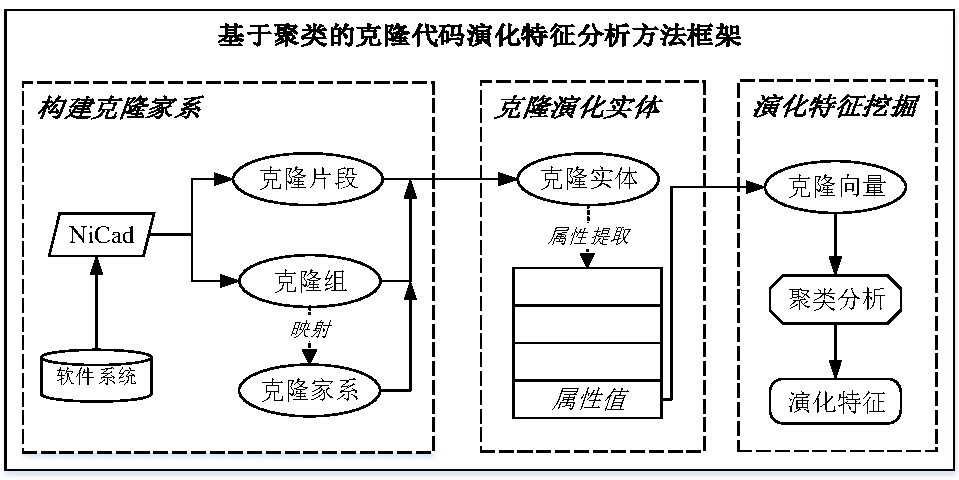
\includegraphics [width=0.7 \textwidth ]{framework2.pdf}
\bicaption [framework2]{}{基于聚类的克隆演化特征提取方法框架}
{Fig.$\!$}{The framework for clone characteristic analysis based on clustering}
\vspace{-1em}
\end{figure}

值得注意的是,本章方法将克隆代码及其演化过程当做一种数据,然后借助机器学习领域中的聚类分析方法挖掘隐含的信息。在使用聚类分析的时候,由于克隆代码是具体的代码片段,无法直接对其聚类。因此,使用克隆聚类向量表示相应的克隆实体,而克隆聚类向量则是根据克隆实体相应的度量值生成,克隆实体的度量值用于表示克隆代码及其演化过程。本文从三种不同克隆实体表示克隆代码,即克隆片段、克隆组和克隆家系。克隆片段实体是微观角度,从克隆代码自身角度出发,将从克隆代码片段本身是否被修改的角度分析克隆代码的演化特征,所提取的度量值重点关注克隆代码是否被修改。克隆组实体是代码区域角度,从克隆组的角度分析克隆代码演化模式与演化时间的关系, 将揭示克隆组在随着软件演化时所表现出来的特征。克隆家系实体是宏观角度,描述了一个系统中所有的克隆代码(即全部克隆家系)的演化过程以及演化特征。

本章所采用的聚类分析方法为{\em X-Means}\cite{pelleg2000x}聚类,其原因在于:克隆实体所应聚类的数量具有不确定性,难以确定具体的聚类数量。如果采用人为给定的方式给出聚类的数量,则可能会引入不客观因素,对影响克隆代码演化特征的分析工作。因此,本章采用\em{ X-Means}聚类方法,不需要人为的指定聚类数量,\em{ X-Means}方法会自动地选择出最佳的聚类数量。

\BiSection{克隆代码演化及其定义}
{The Definitions for Clone Evolution}
\label{lab-evolution}

软件工程实践会产生大量的克隆代码,存在的克隆代码不仅使得系统变得更加臃肿,也使得系统越来越难以理解。为收集和检测系统中存在的克隆代码,在过去的20年中,研究人员提出了许多种克隆代码检测方法,并开发了大量的克隆检测工具,例如NiCad\cite{roy2008nicad}、CCFinder\cite{kamiya2002ccfinder}等(参见本文绪论第~\ref{ref-detection}~节克隆代码检测)。

目前,大多数的克隆检测工具仅可以检测单版本系统中克隆代码,并向程序开发人员报告检测结果。克隆检测结果以克隆片段和克隆组的形式进行组织。克隆片段是具体克隆代码,克隆组是彼此相似的克隆片段的集合。克隆片段和克隆组可以描述如下:

\begin{definition}[克隆片段]
\label{defn-clonefragment}
克隆片段(Clone Fragment, CF)是一段代码片段,包括若干连续的代码行。根据某种相似性,克隆片段与一些其它的代码片段彼此相似,并将它们称之为克隆代码片段,简称为克隆代码。
\end{definition}

\begin{definition}[克隆组]
\label {def-clonegroup}
克隆组 (Clone Group, CG)是彼此相似的克隆片段的集合,包含若干个彼此相似的克隆片段。克隆组揭示了该克隆组内的克隆片段之间的克隆关系,即克隆组内的克隆片段互为克隆关系。
\end {definition}

如绪论中所述,克隆代码在系统中不是静止不变的,会随着软件系统的演化同时进行演化。克隆演化过程最早是2001年由Antoniol等人提出,使用时间序列描述克隆代码的演化模型\cite{antoniol2001modeling},但并未引起人们的重视。2005年,Kim提出了克隆家系模型用于描述克隆代码的演化过程,是迄今为止最好的用于描述克隆代码演化情况的模型\cite{kim2005empirical}。因此,本文也使用克隆家系模型描述克隆代码演化过程。Kim所提出的克隆家系可以描述如下:

\begin{definition}[克隆家系]
\label{def-clonegenealogy}
克隆家系 (Clone Genealogy, CGE)是一个有向无环图,描述了一个克隆组($CG$)随着软件系统进行演化的过程。$CGE$图中的某一节点表示系统某一个版本($V_i$)中的该克隆组($CG_i$)。$CGE$图中的边表示该克隆组($CG$)在相邻的两个版本中$(V_{i-1},V_i )$的演化关系$(CG_{i-1},CG_{i})$,即该克隆组$CG$由上一版本$V_{i-1}$的$CG_{i-1}$演化至下一版本$V_{i}$中的$CG_{i}$。
\end{definition} 

在克隆代码的演化过程中,克隆代码可能会被程序开发人员修改而发生变化,因而也会导致两个相邻版本间的同一克隆组的变化。研究人员使用“克隆演化模式”描述相邻版本之间的克隆组的演化情况。克隆组在两个相邻版本之间的克隆演化模式可以描述如下:

\begin{definition}[克隆演化模式]
\label{def-evolutionpattern}
克隆演化模式 (Clone Evolution Pattern, CEP)是某一克隆组相邻两个软件版本的演化情况。$CEP$描述该克隆组在相邻版本的变化情况,根据不同的演化情况具有7种不同的演化模式。假设该克隆组$CG$从系统版本$V_{i-1}$演化至$V_{i}$,其演化关系$(CG_{i-1},CG_{i})$可以定义如下:
\begin{itemize}
\item 
静态模式 (Static Pattern):
静态模式表示在两个连续版本的演化中该克隆组是静止的,未发生任何变化,即克隆组内的克隆片段数量和内容均未发生变化。
\item 
相同模式(Same Pattern):
相同模式表示在两个连续版本的演化中该克隆组内克隆片段数量无变化,但克隆片段本身可能发生变化。
\item 
增加模式(Add Pattern):
增加模式表示在两个连续版本的演化中该克隆组内的克隆片段数量增加。
\item 
减少模式(Subtract Pattern):
减少模式表示在两个连续版本的演化中该克隆组内的克隆片段数量减少。
\item 
一致性变化模式(Consistent Change Pattern): 
一致性变化模式表示在两个连续版本的演化中该克隆组内的克隆片段发生了一致地变化,并且发生变化的克隆片段仍然存在同一克隆组内。
\item 
不一致性变化模式(Inconsistent Change Pattern):
不一致性变化模式表示在两个连续版本的演化中该克隆组内的克隆片段发生了不一致地变化,并且发生变化的克隆片段仍然存在同一克隆组内。
\item 
分裂模式(Split Pattern):分裂模式表示连续的在两个连续版本的演化中克隆组内克隆片段发生剧烈变化,导致该克隆组分裂成为两个不同的克隆组。
\end{itemize}
\end{definition} 

%%%添加7种演化模式的具体形式化描述。

\begin{figure}[htbp]
\centering
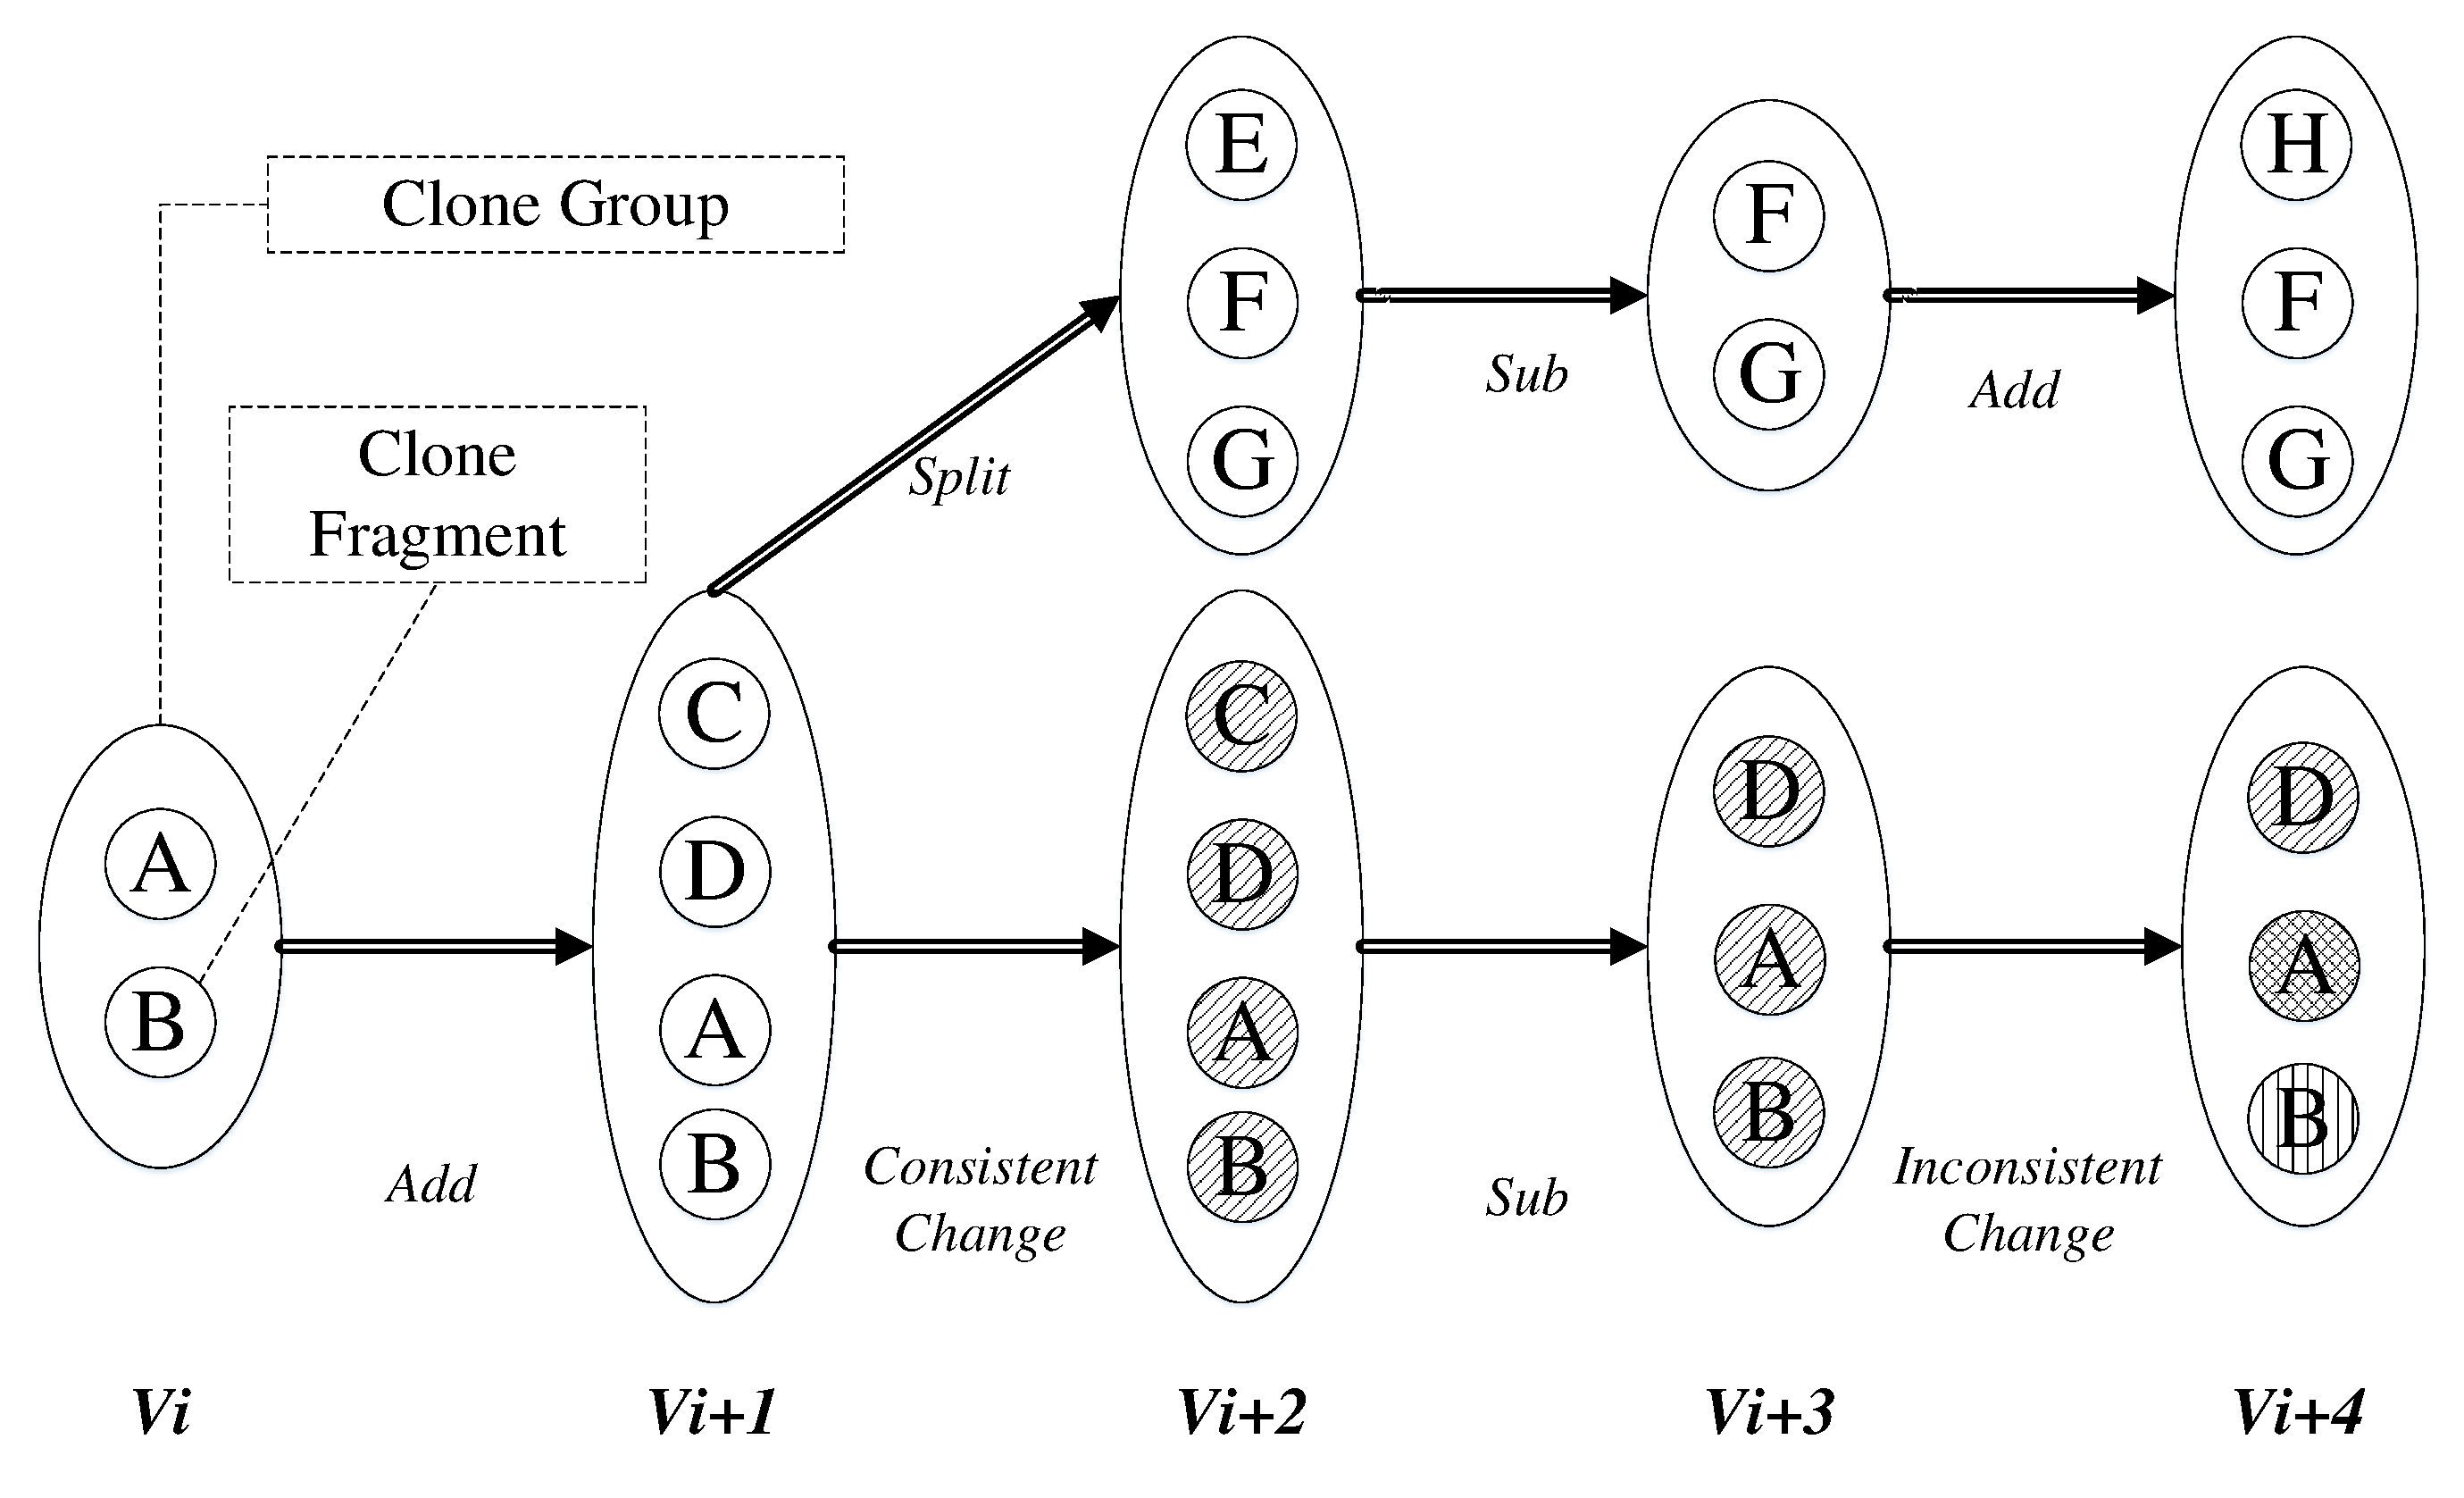
\includegraphics [width=0.7 \textwidth ]{genealogy.pdf}
\bicaption [genealogy]{}{克隆家系示意图}
{Fig.$\!$}{An Example for Clone Genealogy}
\vspace{-1em}
\end{figure}

为了更为形象的描述克隆家系及其演化模式,本文给出一个克隆家系的示意图,如图~\ref{genealogy}~所示。从图中可以看出,克隆家系($CGE$)是克隆组($CG$)随着软件系统演化的一个有向无环图,图的节点表示克隆组$CG$,图中边表示克隆组的演化关系$(CG_{i-1},CG_{i})$,演化模式可以通过比较$CG_{i-1}$和$CG_{i}$中克隆代码片段获取。

图~\ref{genealogy}~同时也描述了一个克隆组$CG$在五个版本$(V_i, V_{i+4})$中的演化过程。从版本$V_i$到$V_{i+1}$,克隆组新增加了两个克隆片段,因此与之其关联的克隆模式是增加模式(Add Pattern)。从 $V_{i+1}$到 $V_{i+2}$中,克隆组首先分裂为两组,因此其演化模式为分裂模式(Split Pattern),同时下方的克隆组发生了相一致的变化,其演化模式为一致性变化模式(Consistent Change Pattern)。从版本$V_{i+2}$到$V_{i+3}$中,演化模式一个是减少模式(Subtract Pattern),另一个是不一致变化模式(Inconsistent Change Pattern)。 从版本$V_{i+2}$到$V_{i+3}$,克隆模式分别是增加模式(Add Pattern)和减少模式(Subtract Pattern)。


\BiSection{构建软件克隆家系}
{Constructing Clone Genealogy for Software}

在构建克隆家系阶段,使用克隆检测工具所检测的连续版本软件中的所有克隆代码,并通过映射相邻版本的克隆代码构建系统的克隆家系。首先,从开源库中下载连续版本软件的所有源代码。然后,使用克隆检测工具NiCad检测克隆代码。最后,通过映射克隆代码构建克隆家系并识别克隆演化模式。

\BiSubsection{克隆检测与结果描述}
{Clone Detection and Results’ Representation}

本节使用克隆检测工具NiCad分别检测系统所有版本中的克隆代码,并使用克隆区域描述符描述克隆代码的相关信息。

为了检测系统中的克隆代码,本文使用{\em NiCad}\cite{roy2008nicad}检测系统中的克隆代码。NiCad是基于文本的克隆检测工具,在工具中集成了程序转换、代码规范化和语法分析技术\cite{cordy2006txl}\cite{dean2003agile},能够以较高的准确度和召回率系统中的Type-1、Type-2和Type-3克隆代码\footnote{NiCad可从此网站获取:http://www.txl.ca/nicaddownload.html。}。NiCad可以从两个不同粒度检测系统中的克隆代码:函数粒度和块粒度。因为块粒度具有更为通用的检测效果(函数克隆也是是块克隆代码),本文使用{块粒度}检测系克隆代码。根据NiCad的默认配置,其将克隆代码之间的相似度阈值设置为70\%,将相似度高于此阈值的代码片段报告为克隆代码。

%%%可以添加相似度计算方法

NiCad将检测到的克隆代码保存于XML文件中,并使用\em{ ``Filename + Start/End Line No.''}标记克隆克隆代码,并将彼此相似的克隆片段保存在同一克隆组内。由于NiCad仅仅使用代码行表示克隆代码,不仅无法描述克隆代码的语法和语义信息,也不利于映射不同版本之间的克隆代码。因此,为映射相邻版本之间的克隆代码,本文使用克隆区域描述符表示克隆代码,并在此基础上实现克隆代码的映射和克隆家系的构建。

克隆区域描述符最早由Duala-Ekoko等人提出,不仅可以反映出克隆代码本身的信息,还可以用于跟踪演化过程中的克隆代码\cite{duala2010clone}。CRD能够充分地反映出克隆代码本身的信息,还能够反映克隆代码区域的特征,CRD的描述如图~\ref{crd}~所示。CRD克服了使用文件行描述克隆代码的局限,不依赖于克隆区域的具体位置,同时也独立于具体文本。使用CRD可以映射相邻版本之间的克隆代码,慈蒙等人改进了克隆区域描述符,并提出了基于克隆区域描述符的克隆群映射算法\cite{ci2013new}\cite{ci2013newD}。同时,为了映射两个相邻版本中的克隆代码和克隆组,新添加相对位置覆盖率和文本相似度两个额外的表示单元。使用相对位置覆盖率可以帮助定位源代码中的克隆片段,并计算版本$i$和版本$i+1$中克隆片段位置之间的重叠率。文本相似度可以用于比较映射的代码片段的相似性度。

%%%%可以添加细节描述

\begin{figure}[htbp]
\centering
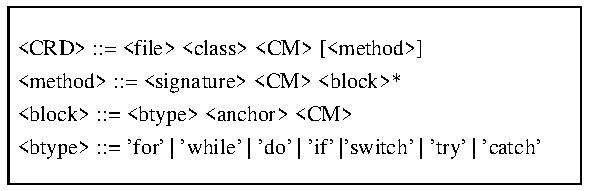
\includegraphics [width=0.5 \textwidth ]{CRD.pdf}
\bicaption [crd]{}{克隆区域描述符示意}
{Fig.$\!$}{The Definition of Clone Region Description}
\vspace{-1em}
\end{figure}

\BiSubsection{克隆家系构建与克隆模式识别}
{Building Clone Genealogy and Identifying Clone Evolutionary Pattern}

为了映射连续版本的克隆代码,使用基于克隆区域描述符的映射算法,生成所有相邻版本的映射结果,并根据映射结果构建克隆家系和识别克隆演化模式。

构建克隆家系的关键步骤在于映射所有相邻版本间的克隆片段。而相邻版本间的克隆群映射关系,则可以根据克隆群内的克隆片段的映射关系进行确定。所采用的映射算法称为基于CRD的克隆代码映射算法\cite{ci2013new}\cite{ci2013newD}。假设给定一个软件系统的两个相邻版本{$V_i$}和{$V_ {i + 1}$},并分别给出两个版本之间的克隆代码,并使用CRD描述所检测到的克隆代码。为了映射两个版本间的克隆代码,将{ $V_i$}中的每个克隆片段与下一版本{$ V_{i+1}$}中的每个克隆片段进行比较,寻找与之映射的克隆片段,并生成克隆片段的映射结果。于此同时,根据克隆片段的映射结果,也可以实现相邻版本中所有克隆组的映射。更进一步,将所有相邻版本之间的克隆代码进行映射,可以通过遍历映射结果生成系统中的所有的克隆家系。

于此同时,克隆演化模式可以用于描述克隆组在演化过程中的变化情况,对于揭示克隆演化特征具有重要的意义。克隆演化模式识别,可以通过对比映射的两个相邻版本之间的克隆组进行。假设克隆组$CG$是存在于相邻的两个软件版本{$(V_i,V_{i+1})$}中,且克隆组$CG$的映射关系可以使用{$(CG_i, CG_{i+1})$}描述,其中{$CG_i$}表示前一版本中的克隆组,{$CG_{i+1}$}表示后一版本中的克隆组。通过观察从{$CG_i$}到{$CG_{i+1}$}的克隆组变化情况,便可以识别该克隆组{$CG_{i+1}$}的克隆演化模式。

\begin{minipage}{0.8\textwidth}
\centering
\begin{algorithm}[H]
\AlgoBiCaption{克隆家系构建与演化模式识别算法} {The algorithm for building clone genealogies and identifying clone evolution patterns}
\label{alg-building}
\KwIn{All software's source code and all code clones with $N$ versions}
\KwOut{All clone genealogies $CGEs$}
%\Comment{生成CRD描述克隆代码片段\;}
\For{$i$=1 to $N$}
{ 
 Generating CRD for represent each $CF_i$ in version $i$\;
 Saving all results in {result\_i} files\;
}
%\Comment{映射相邻版本的$CFs$和$CGs$}
\For{$i$=1 to $N-1$}
{ 
 Mapping all the $CFs$ and $CGs$ between adjacent versions {$i$} and {$i+1$}\;
 Saving all mapping results in {mapping\_i} files\;
}
%\Comment{识别演化模式}
\For{$i$=1 to $N-1$}
{
	\For{each mapping $CGs$ in version $i$ and $i+1$}
	{
	Identify all clone patterns {CEPs} in thus two versions according to Definition~\ref{def-evolutionpattern}~\;
	Saving all mapping results in {mapping\_i} files\;
	}
}
Generating all clone genealogies $CGEs$ through traversing all mapping files\;
\Return {$CGEs$\;}
\end{algorithm}
\end{minipage}

构建克隆家系的算法如~\ref{alg-building}~所示。算法中第1-4行是为所检测到的每一个克隆代码生成CRD描述,并将结果保存。第5-8行是使用基于CRD克隆群映射算法映射相邻版本的克隆代码,同样将结果保存起来。第9-14行根据克隆演化模式定义,识别所有映射的相邻版本的克隆组的克隆演化模式。第15行通过遍历映射文件生成系统中全部的克隆家系。假设一个版本中有$m$个克隆代码,生成CRD所需时间为$O(m)$。软件系统的$n$版本需时间为$O(m*n)$。映射克隆相邻版本的克隆代码以及识别演化模式的时间复杂度同样为$O(m*n)$。所以,该算法的复杂度为$O(m*n)$。

\BiSection{克隆演化实体}
{Three Clone Evolution Entities}

为挖掘克隆代码的演化特征,本节从三个不同的角度表示克隆代码及其演化情况,即克隆片段、克隆组和克隆家系,并将之称为克隆演化实体(简称为克隆实体)。正如在机器学习中通常所做的那样,本节还提取不同的属性值表示克隆代码实体。对克隆片段实体,重点关注克隆代码片段的变化情况。对克隆组实体,重点关注克隆组的克隆演化模式分布情况。对于克隆家系实体,重点关注克隆组在整个演化过程中的演化情况。

\BiSubsection{克隆片段实体}
{Clone Fragment Entity}

克隆代码片段是最小的克隆演化实体单元。克隆片段实体描述了克隆代码本身的一些特征。在克隆片段的生命期间,克隆片段可能被软件人员开发人员修改(特别是在软件维护期间)。因此,克隆片段在演化过程中可能会发生变化,甚至在其演化过程中可能发生不止一次的变化。

因此,对于克隆片段实体,将重点考虑其变化情况。某一版本$V_i$的克隆片段实体,将提取其两个属性表示克隆片段实体,即历史变化次数(截止到版本$V_i$)和是否发生了变化(从上一版本$V_{i-1}$演化到此版本$V_i$时)。同时,也会提取克隆片段实体的寿命作为另一个重要的属性特征。因此,对某一克隆片段实体$CF$,其所在的软件版本为$V_i$,该克隆片段实体$CF_i$的属性值可描述如下:

\begin{itemize}
\item
克隆片段寿命(Clone Fragment Life):
截止到当前版本$V_ i $,克隆片段$CF_i$所经历的所有的版本数量称之为克隆寿命。
%\item {Clone Life}: number of versions which the clone fragment exists in software so far (until version i).
\item
是否发生变化(Ischanged):
从上一版本$V_{i-1} $演化到当前版本$V_ i $时,克隆片段$CF_i$是否发生了变化,若发生变化则取值为$1$,否则取值为$0$。
%\item {Ischanged}:	equals 1 if the Clone fragment in version i is changed from the last version (version i-1); 0 otherwise.
\item
变化次数(Change Times):
截止到当前版本$V_ i $,克隆片段$CF_i$在其演化过程中所发生的变化次数。
%\item {Change Times}:	number of times the clone fragment changed so far (up till version i) in the evolution.  
\end{itemize}

\BiSubsection{克隆组实体}
{Clone Group Entity}

克隆片段实体仅从单个克隆代码的角度描述了克隆演化中的被修改的情况。而克隆组实体可以提供一些克隆代码的区域性特征。克隆代码的变化往往会导致其所在克隆组的变化,可以使用克隆演化模型进行描述。克隆代码演化模式描述了相邻版本之间的克隆组的演化情况,因此,可以使用克隆组当前的演化模式描述克隆组实体的变化情况。

因此,对于某一个演化中的克隆组实体,从上一版本演化至当前版本时,其克隆演化模式可以作为克隆组实体的属性特征。同时,其存在于软件中的时间(克隆组寿命),同样也是一个重要的属性。克隆组寿命不但揭示了其在系统中存在的时间长短,也可能与克隆演化模式息息相关。因此,本节将克隆组的寿命和当前的演化模式视为克隆组实体的属性。对某一克隆组$CG$,其所在的软件文版本为$V_i $ ,该克隆组实体{$CG_i$}的属性值可以描述如下:

\begin{itemize}
\item
克隆组寿命(Clone Group Life):
截止到当前版本$V_ i $,克隆组$CG_i$所经历的所有的版本数量称之为克隆寿命。
%\item {Group Life}: number of versions which clone group exists in software till version $i$.
\item
当前静态模式(Current Static Pattern):
克隆组$CG_i$从上一版本$V_{i-1} $演化到$V_i $时,是否发生了静态模式(Static Pattern)。
%\item {Static}:	all clone fragments in group are static from last version.
\item
当前相同模式(Current Same Pattern):
克隆组$CG_i$从上一版本$V_{i-1} $演化到$V_i $时,是否发生了相同模式(Same Pattern)。
%\item {Same}:	clone group undergoes a ``same'' pattern change from  last version.
\item
当前增加模式(Current Add Pattern):
克隆组$CG_i$从上一版本$V_{i-1} $演化到$V_i $时,是否发生了增加模式(Add Pattern)。
%\item {Add}: clone group undergoes an ``add'' pattern change from last version.
\item
当前减少模式(Current Subtract Pattern):
克隆组$CG_i$从上一版本$V_{i-1} $演化到$V_i $时,是否发生了减少模式(Subtract Pattern)。
%\item {Subtract}: clone group undergoes a ``subtract'' pattern change from last version.
\item
当前一致性变化模式(Current Consistent Change Pattern):
克隆组$CG_i$从上一版本$V_{i-1} $演化到$V_i $时,是否发生了一致性变化模式(Consistent Change Pattern)。
%\item {Consistent Change}: clone group undergoes a ``consistent change'' pattern from last version.
\item
当前不一致变化模式(Current Inconsistent Change Pattern):
克隆组$CG_i$从上一版本$V_{i-1} $演化到$V_ i $时,是否发生了不一致变化模式(Inconsistent Change Pattern)。
%\item {Inconsistent Change}: clone group undergoes an ``inconsistent change'' pattern from last version.
\item
当前分裂模式(Current Split Pattern):
克隆组$CG_i$从上一版本$V_{i-1} $演化到$V_i $时,是否发生了分裂模式(Split Pattern)。
%\item {Split}: clone group undergoes a ``split'' pattern change from last version.
\end{itemize}

\BiSubsection{克隆家系实体}
{Clone Genealogy Entity }

克隆家系实体是克隆代码演化的全局视角。该实体提供了某一克隆组在其整个演化过程中的演化情况,可以帮助捕获软件系统中全部克隆代码的演化情况。如前文所述,一个克隆组在所有的版本中的全部演化过程是一个克隆家系。因此,在其整个演化过程中,其所经历的所有的演化模式数量,可以描述克隆家系实体的在其整个演化过程中的整个变化历史演化过程。同时,对于一个克隆家系,克隆寿命是克隆家系的另一个重要的指标,描述了克隆代码在系统中存在的时间。

因此,克隆家系实体的寿命和克隆演化模式数量可以作为克隆家系实体的属性。对于某一克隆家系实体{$CGE$},该克隆家系实体{$CGE$}的属性值可以描述如下:

\begin{itemize}
\item
克隆家系寿命(Clone Genealogy  Life):
克隆家系{$CGE$}在其整个演化过程中所经历的软件版本的数量。
%\item Genealogy  Life: number of versions which clone genealogy exists in software.
\item
静态模式数量(Static Pattern Number):
克隆家系{$CGE$}在其整个演化过程中所经历的静态模式的数量。
%\item Static Number: number of ``static'' pattern which all clone groups belonging to this genealogy have experienced in its life.
\item
相同模式数量(Same Pattern Number):
克隆家系{$CGE$}在其整个演化过程中所经历的相同模式的数量。
%\item Same Number: number of ``same'' pattern which all clone groups belonging to this genealogy have experienced in its life.
\item
增加模式数量(Add Pattern Number):
克隆家系{$CGE$}在其整个演化过程中所经历的增加模式的数量。
%\item Add Number: number of ``add'' pattern which all clone groups belonging to this genealogy have experienced  in its life.
\item
减少模式数量(Subtract Pattern Number):
克隆家系{$CGE$}在其整个演化过程中所经历的减少模式的数量。
%\item Subtract Number: number of ``subtract'' pattern which all clone groups belonging to this genealogy have experienced in its life.
\item
一致性变化模式数量(Consistent Change Pattern Number):
克隆家系{$CGE$}在其整个演化过程中所经历的一致性变化模式的数量。
%\item Consistent Number: number of ``consistent pattern'' which all clone groups belonging to this genealogy have experienced in its life.
\item
不一致变化模式数量(Inconsistent Change Pattern Number):
克隆家系{$CGE$}在其整个演化过程中所经历的不一致变化模式的数量。
%\item Inconsistent Number: number of ``inconsistent pattern'' which all clone groups belonging to this clone genealogy have experienced in its life.
\item
分裂模式数量(Split Pattern Number):
克隆家系{$CGE$}在其整个演化过程中所经历的分裂模式的数量。
%\item Split Number: number of ``split'' pattern which all clone groups belonging to this genealogy have experienced in its life.
\end{itemize}

\BiSection{克隆演化特征挖掘}
{Mining Clone Evolutionary Characteristics}

为了从克隆代码及其演化过程中挖掘演化特征,上一节使用不同的属性值分别描述克隆代码实体、克隆组实体和克隆家系实体。在上一节的基础上,本节将使用WEKA( “Waikato Environment for Knowledge Analysis” \cite{hall2009weka})中提供的聚类方法来分析克隆演化实体,将从克隆片段、克隆组和克隆家系三个不同的角度分别对克隆代码及其演化过程进行聚类分析。

\BiSubsection{生成克隆实体聚类向量空间}
{Generating the Space of Clustering Vectors for Clone Entities}

使用X-means聚类克隆代码实体,需要生成与之对应的克隆聚类向量空间。这一过程可以划分为两个子步骤:首先,为每一个克隆代码实体成一个“克隆聚类向量”,该向量包含某个克隆实体的所有属性值。然后,使用克隆实体全部的“克隆聚类向量”生成所有克隆实体的“聚类空间”,包含克隆片段、克隆组和克隆家系三个聚类空间。

(1)为每一个克隆代码实体生成克隆聚类向量。 

对于每个克隆片段、克隆组和克隆家系实体,其聚类向量是一个$m$维向量$Vector$:即{$Vector$ ={($v_1$,$v_2$,$...$,$v_m$)}},其中$v_i$表示该克隆实体的一个特定属性值。以某一克隆组{$CG_i$}为例,为该克隆组实体{$CG_i$}生成一个8维向量{$Vector(CG_i)$ = ($v_1$,$v_2$,$...$,$v_8$)},其中$v_i$(对于所有$i$ , $i \leq $ 8)是此克隆组{$CG_i$}所对应的属性值。$Vector(CG_i)$即为克隆组实体{$CG_i$}的克隆聚类向量。
 
(2)生成所有克隆代码实体的聚类向量空间。

为了聚类所有的克隆实体,还行生成系统的全部克隆聚类向量空间。假设由所有克隆实体的聚类向量生成的聚类向量空间为$X$,则$X$可由{$X$={($x_1$,$x_2$,$...$,$x_n$)}}表示,其中$n$是全部克隆实体的数量。本章从克隆片段实体、克隆组实体和克隆家系实体三个不同角度,聚类分析克隆代码及其演化过程。因此,本节也将生成三个不同的克隆向量空间:$X_{CF}$、$X_{CG}$和$X_{CGE}$,其中$X_{CF}$表示所有的克隆片段实体的聚类空间,$X_{CG}$表示所有克隆组实体的聚类空间,$X_{CGE}$表示所有克隆家系实体的聚类空间。

\BiSubsection{使用X-means聚类克隆实体}
{Clustering All Clone Entities with X-means Method}

使用X-means方法聚类所有的克隆实体向量($X_{CF}$、$X_{CG}$和$X_{CGE}$),并根据聚类结果分析和提取克隆代码演化特征。

本章将使用WEKA中实现的聚类方法,实现对克隆实体的聚类。WEKA是一个用于数据挖掘的流行机器学习工具,WEKA中实现了许多方法来分析数据,例如聚类,分类,关联规则等\footnote{WEKA是新西兰怀卡托大学用Java开发的数据挖掘软件工具,其几乎可以运行在所有操作系统平台上。其网站是:http://www.cs.waikato.ac.nz/ml/weka/}。 由于上一节所生成克隆代码的向量空间为$X_{CF}$、$X_{CG}$和$X_{CGE}$,分别代表了系统中全部的克隆片段实体、克隆组实体和克隆家系实体。因此,也将使用X-means方法聚类这三个不同的向量空间,并分析得到克隆代码的演化特征。

本文使用的聚类方法是X-means聚类\cite{pelleg2000x}, X-means聚类是K-means聚类\cite{arthur2007k}的改进方法。后者可以将向量空间$X$聚类为事前指定的$K$个Cluster中,并将彼此相似的向量分配到同一个Cluster中。但是,K-means聚类方法必须指定所需要聚类的Cluster的数量。然而,对于克隆代码演化的聚类而言,由于缺少必要的基本信息,难以确定所需的Cluster的数目。因此,本章选择使用X-means聚类方法。X-means聚类改进了K-means聚类方法,聚类时并不需要指定具体的Cluster数量。X-means聚类会自动的搜索最佳的Cluster数量,因此更为适合于克隆代码演化特征的聚类分析。

X-means聚类是一种高效的聚类算法,可以通过自动搜索并确定聚类数量\cite{pelleg2000x}。给定一个克隆实体的克隆向量空间$X$ = {($x_1$,$x_2$,$...$,$x_n$)},其中每个$x_i$是$d$维克隆演化实体的向量)。X-means聚类将向量空间$X$ 中的$n$个向量划分为$k$个Clusters,即 $C$ = {($c_1$,$c_2$,$...$,$c_k$)},$c_i$表示一个Cluster。$c_i$则表示了彼此比较相似的克隆代码实体,根据聚类结果可以进行克隆演化特征的挖掘。使用X-means聚类仅需要指定$K$的范围即可,聚类算法会自动的搜索最佳的Cluster数量$K$。聚类分析的结果见后文的实验分析部分。

最后,根据聚类分析的结果,可以进行挖掘和分析克隆代码的演化特征。

%%%描述X-means聚类
%过程如下:算法从给定的$K$范围的最低值开始,并继续增加此值,直到范围的上限。在此过程中,X-means聚类使用模型选择标准计算每个$K$的分数。它选择$K$的最高分数输出。对于每个$K$,x-means聚类使用迭代细化技术。首先,它将每个向量分配给其平均值产生集群内最小平方和(WCSS)的集群。第二,它计算新的均值为新聚类中的向量的质心。当分配不再改变时,算法收敛。它使用后验概率用贝叶斯信息准则对这$j$进行评分。

克隆演化特征的聚类算法如~\ref{alg-characteristic}~所示。算法的第1-3行分别收集系统中全部的克隆实体,分别为克隆家系实体、克隆组实体和克隆片段实体。第4行初始化三种克隆实例的聚类向量空间。第5-8行、9-12行、13-16行分别使用上文描述的属性生成克隆实体的聚类向量,并将其添加到聚类向量空间中。最后,第17行调用WEKA聚类克隆实体。收集不同克隆实体的算法复杂度为$O(m)$。算法的主要时间消耗在了生成克隆实例的向量空间上,其时间复杂度为$O(n*m)$,$n$为系统的版本数量。所以,该算法的时间复杂度为$O(n*m)$。

\begin{minipage}{0.8\textwidth}
\centering
\begin{algorithm}[H]
\AlgoBiCaption{克隆演化特征聚类算法} {The algorithm of clustering for clone characteristics}
\label{alg-characteristic}
\KwIn{All clone genealogies $CGEs$ and all source code}
\KwOut{All the clusters for clone fragments, groups, and clone genealogies}
Collecting all entities of clone genealogy with number {$N\_cge$}\;
Collecting all entities of clone group with number{$N\_cg$}\;
Collecting all entities of clone fragment with number {$N\_cf$}\; 
Initializing the clustering space of  $X_{CF}$, $X_{CG}$, and $X_{CGE}$\;
\For {$i$=1 to $N\_cge$}
{
 Generating the vector {$V\_i$} for {CGE\_i}\;
 Appending the vector {$V\_i$} to $X_{CGE}$\;
 }
\For {$i$=1 to $N\_cg$}
{ 
 Generating the vector for {CG\_i}\;
 Appending the vector {$V\_i$} to $X_{CG}$\;
}
\For {$i$=1 to $N\_cf$}
{ 
 Generating the vector {$V\_i$} for{CF\_i}\;
 Appending the vector {$V\_i$} to $X_{CF}$\;
}
Calling WEKA to clustering $X_{CF}$, $X_{CG}$ and  $X_{CGE}$ with X-means method\;
Mining clone evolutionary characteristic with the clusters of $X_{CF}$, $X_{CG}$ and  $X_{CGE}$\;
\Return {All the clusters for clone fragment, group, and genealogy\;}
\end{algorithm}
\end{minipage}

\BiSection{克隆代码演化特征实验结果与分析}
{The Results and Discussion for Clone Evolutionary Characteristics}
\label{ref-characteristics}

\BiSubsection{实验系统和实验设置}
{Experimental Projects and Methodology}

本章选择了两个开源软件作为本章的实验系统:分别为ArgoUML和 jEdit。ArgoUML是一个领先的开源UML建模工具,包括对所有标准UML 1.4图的支持。jEdit是程序员开发所使用的编辑器,其特点是具有易于使用的接口,类似于许多流行的文本编辑器。

表~\ref{statisticsofcluster}描述了这两个实验系统的基本信息。从表中第2-4列给出了系统的版本信息,ArgoUML经历了$14 $个版本的演化(起始和结束版本分别为$0.20.0$和$0.34.0$), jEdit经历了$22$个版本的演化(起始和结束版本分别为$3.0.0$和$5.0.0$)。表中第5-7列则给出了实验系统的克隆实体的数量(即克隆聚类空间大小)。其中,“Clone Fragment”列出了所聚类的克隆片段的数量,“Clone Group”和“Clone Genealogy”则分别是所聚类的克隆组和克隆家系数量。

\begin{table}[htbp]
\bicaption [statisticsofcluster]{}{两个开源软件实验系统信息}
{Table$\!$}{The information of two open sources experimental projects }
\vspace{0.5em}
\centering 
\wuhao
\begin{tabular}{ccccccc}
\toprule[1.5pt ]
\multirow{2}{*}{实验系统}&\multirow{2}{*}{版本数}&Start&End&Clone&Clone&Clone\\ 
&&Version&Version&Fragment&Group&Genealogy\\
\midrule[1pt]
ArgoUML&14&0.20.0&0.34.0&25422&7012&1036\\ 
jEdit&22&3.0.0&5.0.0&6636&2256	&237\\ 
\bottomrule[1.5pt]
\end{tabular}
\end{table}

本章从三个不同的视角挖掘和分析克隆代码的演化特征,即克隆片段、克隆组和克隆家系。因此,克隆演化特征的实验也可以划分成为三个部分,分别为:
\begin{itemize}
\item 克隆片段演化特征分析实验:
在克隆片段实验中,聚类克隆片段实体的向量空间,将分析克隆片段在演化过程中的变化情况,挖掘克隆片段变化的演化特征。 
\item 克隆组演化特征分析实验:
在克隆组实验中,聚类克隆组实体的向量空间,将分析克隆组在演化过程中的克隆演化模式情况,并挖掘克隆组实体的一致性和不一致变化模式。
\item 克隆家系演化特征分析实验:
在克隆家系的实验中,聚类克隆家系实体的向量空间,从全局的角度分析了系统中全部克隆代码的演化规律,并挖掘在整个演化过程中克隆代码的稳定性以及一致性变化的演化特征。
\end{itemize}

在每个实验中,又将克隆代码演化特征的挖掘分成两个子任务:第一,对获得的所有克隆实体进行统计分析,并且根据统计分析结果获取克隆代码的演化特征。第二,使用WEKA对克隆实体进行聚类分析,根据聚类结果获取克隆代码的演化特征。因此,使用均使用两种方法分析和挖掘克隆代码的演化特征:统计分析和聚类分析。第一种统计分析每种克隆实体的属性值分布情况,进而发现一些基本的分布特征。第二种是聚类分析方法,使用X-means分别聚类每一种克隆实体,并根据聚类结果深入挖掘在演化中克隆代码的演化特征。

\BiSubsection{克隆片段演化特征分析实验}
{Experiment for Clone Fragment Evolutionary Characteristics}

克隆片段是软件中存在的真实的代码片段, 在其生命周期内,克隆片段可能会被开发人员修改。考虑克隆片段实体的三个属性特征,分别是克隆寿命(Clone Life)、是否发生变化(Ischanged)和历史变化次数(Change Times),将帮助挖掘克隆片段在其演化过程中的真实变化情况。

\BiSubsubsection{克隆片段统计分析实验}
{Clone Fragment Experiment of Statistics}

对克隆片段“历史变化次数”进行统计分析,分析结果如表~\ref{cfstaargouml}~和表~\ref{cfstajedit}~所示。表中统计了克隆代码片段的变化情况,其中数字“$0$”表示从未发生变化,数字“$N$”表示了截止到当前版本克隆片段发生了N次变化。

从表~\ref{cfstaargouml}~和表~\ref{cfstajedit}~中可以看出,大多数克隆片段在演化过程中并不会发生变化。未发生变化的克隆片段数量在ArgoUML中为$24327$个,在jEdit中为$5885$。同时,只有仅仅一小部分克隆片段在演化过程中发生了变化(ArgoUML为$1095$个,jEdit为$751$个)。值得注意的是,在发生变化的克隆片段中,仅有极少数的克隆片段被改变了不止一次,其数量随着改变次数的增大而减少。

 因此可以得出结论:克隆片段在其生命期间是十分稳定的,大多数克隆片段从未发生变化。但是,依然存在一定数量的克隆代码片段发生了变化。在发生变化的克隆片段中,克隆变化不会频繁地发生,仅有极少量的克隆代码会频繁的发生变化。

\begin{table}[htbp]
\bicaption[cfstaargouml]{}{ArgoUML中克隆片段的变化情况统计}
{Table$\!$}{The statistic of clone fragment change for ArgoUML}
\vspace{0.5em}
\centering
\wuhao
\begin{tabular}{ccccc}
\toprule[1.5pt]
Change Times&0&1&2&3\\ 
\midrule[1pt]
数量&24327&982&109&4\\ 
\cline{3-5}
总数&24327&\multicolumn{3}{c}{1095} \\
\bottomrule[1.5pt]
\end{tabular}
\end{table}

\begin{table}[htbp]
\bicaption[cfstajedit]{}{jEdit中克隆片段的变化情况统计}
{Table$\!$}{The statistic of clone fragment change for jEdit}
\vspace{0.5em}
\centering
\wuhao
\begin{tabular}{ccccccccc}
\toprule[1.5pt]
Change Times &0&1&2&3&4&5&6&7\\ 
\midrule[1pt]
数量&5885&533&135&47&14&10&11&1\\ 
\cline{3-9}
总数&5885&\multicolumn{7}{c}{751}   \\ 
\bottomrule[1.5pt]
\end{tabular}
\end{table}

\BiSubsubsection{克隆片段聚类分析实验}
{Clone Fragment Experiment of Clustering}

使用X-means方法对克隆片段进行聚类分析,实验结果如表~\ref{cfcluargouml}~和~\ref{cfclujedit}~所示。从表中可以看出,X-means聚类将ArgoUML和jEdit的克隆代码片段实体分成4个Cluster:Cluster0-Cluster3。根据其聚类结果分别统计了四个Cluster的属性特征的信息,并使用平均值(Mean)、标准差(Standard Deviation,SD)和中位数(Median)来描述每一个Cluster中的属性的分布情况。

从表中可以看出,在ArgoUML和jEdit两个系统中,Cluster0的克隆片段中数量最少,该Cluster中的克隆代码在其演化的过程中发生过变化(Change Times约等于1),将这些克隆片段称为“发生变化的”(changed)克隆片段。因此,在所有的克隆代码片段中仅有少量的克隆代码片段发生过变化。同时,相对于未发生变化的克隆代码(Cluster3,ischanged和Change Times均为0),克隆代码发生变化的时刻往往是其存在于系统中一段时间后(Cluster0的Clone Life数值要大于Cluster3的Clone Life)。

除此之外,根据“isChanged”列可以看出,在系统ArgoUML中的Cluster1、Cluster3和系统jEdit中的Cluster1、Cluster2和Cluster3中,所有的克隆片段都没有发生变化将它们称为“未发生变化”的克隆代码片段。对于未发生变化的克隆代码片段,从表中第2列(数量和比例)可以看出,该类克隆代码片段,占到全部克隆片段数量的大多数。这意味着大多数的克隆片段在其演化的过程中是稳定的,不会发生变化。

最后,系统ArgoUML和jEdit中的Cluster3是完全没有发生变化的克隆片段,根据其寿命发现它们在软件中存在的时间极短 。这表明刚刚出现在系统中的克隆是极其稳定的(在短时间内不会发生变化)。因此,程序开发人员应该更多地关注那些已经存在系统中一段时间(存在几个版本)的克隆代码片段,因为它们更容易发生变化。

综上所述,只有少数的克隆代码片段在软件演化过程中会发生变化,同时这些克隆片段所经历的变化通常发生在它们在系统中存在一段时间之后。

\begin{table}[htbp]
\bicaption[cfcluargouml]{}{ArgoUML中克隆片段的聚类结果}
{Table$\!$}{Clustering results of clone fragment for ArgoUML}
\vspace{0.5em}
\centering
\footnotesize
%\wuhao
\begin{tabular}{ccccccccccc}
\toprule[1.5pt]
\multirow{2}{*}{Cluster}&{数量}&\multicolumn{3}{c}{Clone Life}&\multicolumn{3}{c}{Ischanged}&\multicolumn{3}{c}{Change Times} \\
\cline{3-11}
&(比例)&{Mean}&SD &{Median}&{Mean}&SD &{Median}&{Mean}&SD &{Median}\\
\midrule[1pt]
Cluster 0&899(4\%)&7.207&2.299&7&0.092&0.290&0&1.130&0.350&1\\ 
Cluster 1&3082(12\%)&7.763&1.523&8&0&0&0	&0&0&0\\ 
Cluster 2&3006(12\%)&3.833&0.871&4&0.058&0.234&0	&0.065&0.247&0\\ 
Cluster 3&18435(73\%)&1.094&0.292&1	&0	&0	&0	&0	&0	&0\\ 
\bottomrule[1.5pt]
\end{tabular}
\end{table}

\begin{table}[htbp]
\bicaption[cfclujedit]{}{jEdit中克隆片段的聚类结果}
{Table$\!$}{Clustering results of clone fragment for jEdit}
\vspace{0.5em}
\centering
\footnotesize
%\wuhao
\begin{tabular}{ccccccccccc}
\toprule[1.5pt]
\multirow{2}{*}{Cluster}&{数量}&\multicolumn{3}{c}{Clone Life}&\multicolumn{3}{c}{Ischanged}&\multicolumn{3}{c}{Change Times} \\
\cline{3-11}
&(比例)&{Mean}&SD &{Median}&{Mean}&SD&{Median}&{Mean}&SD &{Median}\\
\midrule[1pt]
Cluster 0&200(3\%)&5.325&2.690&5&1	&0	&1	&1.64	&1.148&1\\ 
Cluster 1&1371(21\%)	&9.071&2.885&8	&0	&0	&0	&0.503&0.916&0\\ 
Cluster 2&	1624(15\%)	&4.227&1.112&4	&0	&0	&0	&0.065&0.261&0\\ 
Cluster 3&	3441(66\%)	&1.175	&0.3780&1	&0	&0	&0	&0	&0	&0\\ 
\bottomrule[1.5pt]
\end{tabular}
\end{table}

%%%%以下是未保留小数的实验结果
%%\begin{table}[htbp]
%%\bicaption[cfcluargouml]{}{ArgoUML中克隆片段的聚类结果}
%%{Table$\!$}{Clone Fragment Clustering Results of ArgoUML}
%%\vspace{0.5em}
%%\centering
%%\wuhao
%%\begin{tabular}{ccccccccccc}
%%\toprule[1.5pt]
%%\multirow{2}{*}{Cluster}&{Number}&\multicolumn{3}{c}{Clone Life}&%%\multicolumn{3}{c}{Ischanged}&\multicolumn{3}{c}{Change Times} \\
%%&(Percentage)&{Mean}&SD &{Median}&{Mean}&SD &{Median}&{Mean}&SD %%&{Median}\\
%%%%%\multirow{3}{*}{Cluster}&{Number}&\multicolumn{3}{c}{Clone Life}&\multicolumn{3}{c}{Ischanged}&\multicolumn{3}{c}{Change Times} \\
%%%%%%%&(Percentage)&\multirow{2}{*}{Mean}& Standard &\multirow{2}{*}{Median}&\multirow{2}{*}{Mean}&Standard &\multirow{2}{*}{Median}&\multirow{2}{*}{Mean}&Standard &\multirow{2}{*}{Median}\\
%%%%%&&&  Deviation&&& Deviation&&& Deviation&\\ 
%%\midrule[1pt]
%%Cluster 0&899(4\%)&7.2069&2.2993&7&0.09232&0.28965&0&1.13014&0.34963&1\\ 
%%Cluster 1&3082(12\%)&7.76314&1.52307&8&0&0&0	&0&0&0\\ 
%%Cluster 2&3006(12\%)&3.833&0.8707&4&0.05822&0.23419	&0	&0.0652&0.24692&0\\ 
%%Cluster 3&18435(73\%)&1.09401&0.29184	&1	&0	&0	&0	&0	&0	&0\\ 
%%\bottomrule[1.5pt]
%%\end{tabular}
%%\end{table}

%%\begin{table}[htbp]
%%\bicaption[cfclujedit]{}{jEdit中克隆片段的聚类结果}
%%{Table$\!$}{Clone Fragment Clustering Results of jEdit}
%%\vspace{0.5em}
%%\centering
%%\wuhao
%%\begin{tabular}{ccccccccccc}
%%\toprule[1.5pt]
%%\multirow{2}{*}{Cluster}&{Number}&\multicolumn{3}{c}{Clone Life}&\multicolumn{3}{c}{Ischanged}&\multicolumn{3}{c}{Change Times} \\
%%&(Percentage)&{Mean}&SD &{Median}&{Mean}&SD&{Median}&{Mean}&SD &{Median}\\
%%%%%\multirow{3}{*}{Cluster}&{Number}&\multicolumn{3}{c}{Clone Life}&\multicolumn{3}{c}{Ischanged}&\multicolumn{3}{c}{Change Times} \\
%%%%%&(Percentage)&\multirow{2}{*}{Mean}& Standard &\multirow{2}{*}{Median}&\multirow{2}{*}{Mean}&Standard &\multirow{2}{*}{Median}&\multirow{2}{*}{Mean}&Standard &\multirow{2}{*}{Median}\\
%%%%%&&&  Deviation&&& Deviation&&& Deviation&\\ 
%%\midrule[1pt]
%%Cluster 0&	200(3\%)	&5.325	&2.6899	&5	&1	&0	&1	&1.64	&1.1476	&1\\ 
%%Cluster 1&	1371(21\%)	&9.07075	&2.88542	&8	&0	&0	&0	&0.50328	&0.91649	&0\\ 
%%Cluster 2&	1624(15\%)	&4.2266	&1.11192	&4	&0	&0	&0	&0.06466	&0.26059	&0\\ 
%%Cluster 3&	3441(66\%)	&1.17495	&0.37998	&1	&0	&0	&0	&0	&0	&0\\ 
%%\bottomrule[1.5pt]
%%\end{tabular}
%%\end{table}

\BiSubsection{克隆组演化特征分析实验}
{Experiment for Clone Group Evolutionary Characteristics}

克隆片段实体仅提供了克隆片段本身的变化情况,而通过对克隆组实体进行实验分析,则可以提供了克隆代码以克隆组为单位的在两个相邻版本的演化情况。 在克隆组实体实验中,通过统计和聚类克隆组在演化过程中的克隆演化模式,可以揭示克隆代码的演化特征。

\BiSubsubsection{克隆组统计分析实验}
{Clone Group Experiment of Statistics} 

统计克隆组实体的“克隆演化模式”(Clone Pattern)分布情况,其结果如表~\ref{cgstaargouml}~和~\ref{cgstajedit}~所示。表中第二行和第三行使用“Present”和“Absent”来标识某一克隆组实体是否具有某种具体克隆演化模式。其中,“Present”表示拥有某演化模式,“Absent”表示没有\footnote{克隆组的演化模式之间不是相互独立的,一个克隆组可以具有多个演化模式,例如可以同时具有“Static”和“Same”。}。同时,本节也非正式地将克隆演化模式中“Static”模式和“Same”模式称为“稳定的克隆演化模式”(Stable Clone Pattern),其它的克隆模式称为“动态的克隆模式”(Dynamic Clone Pattern)。表中最后一行给出具有某一克隆演化模式的克隆组实体的比例。

从表中可看出,在两个实验系统中,大多数的克隆组实体(比例约72\% - 85\%)具有有稳定的克隆演化模式(“Static”和“Same”。),只有一小部分克隆组(其比例小于7\%)具有动态的克隆模式,即拥有“Add”,“Sustract”,“Split”,“Consistent/Inconsistent Change”模式。

值得注意的是,在ArgoUML和jEdit中有数百个克隆组实体具有Consistent/Inconsistent Change模式。这应该引起程序开发人员的注意,因为这种变化模式----特别是一致性变化模式(Consistent Change)----会导致额外的维护代价甚至会引发相关的克隆缺陷。在这些发生变化的克隆组实体中,在系统jEdit和ArgoUML中,发生一致变化(Consistent Change)模式的克隆组要多于不一致变化(Inconsistent Change)模式的克隆组。ArgoUM具有两种模式克隆组数量分别为:$350$和$329$,jEdit为$140$和$41$。

因此可以得出结论:相比于不一致变化模式,软件系统中的克隆组更容易发生一致性的变化。

\begin{table}[htbp]
\bicaption[cgstaargouml]{}{ArgoUML中克隆组的演化模式统计}
{Table$\!$}{The statistic of clone group evolution pattern for ArgoUML}
\vspace{0.5em}
\centering
\wuhao
\begin{tabular}{cccccccc}
\toprule[1.5pt]
~&\multirow{2}{*}{Static}&\multirow{2}{*}{Same}&\multirow{2}{*}{Add}&\multirow{2}{*}{Subtract}&Consistent&Inconsistent&\multirow{2}{*}{Split}\\ 
~&&&&&Change&Change&\\ 
\midrule[1pt]
Present	&5114	&5422	&345	&324	&350	&329	&36\\ 
Absent	&1898	&1590	&6667	&6688	&6662	&6683	&6976\\ 
比例	&72.93\%	&77.40\%	&4.92\%	&4.62\%	&5.25\%	&4.69\%	&0.51\%\\ 
\bottomrule[1.5pt]
\end{tabular}
\end{table}

\begin{table}[htbp]
\bicaption[cgstajedit]{}{jEdit中克隆组的演化模式统计}
{Table$\!$}{The statistic of clone group evolution pattern for jEdit}
\vspace{0.5em}
\centering
\wuhao
\begin{tabular}{cccccccc}
\toprule[1.5pt]
~&\multirow{2}{*}{Static}&\multirow{2}{*}{Same}&\multirow{2}{*}{Add}&\multirow{2}{*}{Subtract}&Consistent&Inconsistent&\multirow{2}{*}{Split}\\ 
~&&&&&Change&Change&\\ 
\midrule[1pt]
Present	&1783	&1922	&45	&36	&140	&41	&19\\ 
Absent	&473	&334	&2211	&2220	&2116	&2215	&2237\\ 
比例	&79.3\%	&85.20\%	&1.99\%	&1.60\%	&6.21\%	&1.82\%	&0.84\%\\ 
\bottomrule[1.5pt]
\end{tabular}
\end{table}

\BiSubsubsection{克隆组聚类分析实验}
{Clone Group Experiment of Clustering} 

使用X-means方法对克隆组实体进行聚类分析,聚类分析的结果如表~\ref{cgcluargouml}~和~\ref{cgclujedit}~所示。与克隆片段聚类实验相似,聚类结果也分成了四类:Cluster0-3。相似地,也分别统计了每一Cluster中的克隆组实体的演化模式的分别情况,并使用“Mean”表示平均值、“SD”表示标准差、“Median”表示中位数。

从上述两个表中可以看出,Cluster1的克隆组实体的数量最多(在ArgoUML中比例为71\%,在jEdit中占79\%)。Cluster1的克隆组比较稳定(克隆组具有稳定的克隆模式,并且没有动态的克隆模式),同时具有相对较长的寿命。因此,大多数的克隆组是非常稳定的,也具有相对较长的寿命(在两个软件中大约5个版本)。

从表中还可以看出,Cluster0和Cluster2都是动态克隆组,因为这些克隆组实体都具有动态的克隆演化模式。在发生变化的克隆组实体中,大多数的不一致变化模式(Inconsistent Change Pattern)出现在Cluster0中,并且仅仅占用很小的比例(ArgoUML中的4\%,在jEdit中只有1\%)。因此可以得出结论不一致变化模式在克隆组中不会频繁发生。值得注意的是,一致性变化模式(Consistent Change Pattern)仅发生在Cluster2中,其存在的克隆组的寿命相对较长,但相比于Cluster0会短一些。因此得出结论:动态的克隆演化模式往往会发生在较为长寿的克隆组实体中,但是它们的数量也会非常小。

从Cluster0 和Cluster2中克隆组的绝对数量上看,具有一致性变化模式(Consistent Change Pattern)的克隆组(Cluster2)的数量大于具有不一致变化模式(Inconsistent Change Pattern)的克隆组数量(Cluster0)。这意味着一致性变化模式相比于不一致性变化模式更容易发生。因此,建议开发人员在修改克隆组中某一克隆片段时需要考虑同时修改组内其它的克隆片段,即考虑克隆代码的一致性变化问题。

最后,从Cluster3中可以看出,有相当一部分的克隆组具有极短的寿命(刚刚出现在系统中),因此其并没有相关的克隆演化模式。这也意味着在克隆组刚刚创建的初始版本中并不不需要考虑克隆组的变化情况以及对系统的影响问题。

综上所述,克隆组在其演化过程中通常是非常稳定的。当克隆组存在于系统的一段时间之后,动态的克隆演化模式可会发生在一小部分的克隆组中。同时,当开发人员修改某一克隆片段时,本文建议需要考虑克隆组内其它克隆片段是否需要一致性修改,即确定克隆组变化的一致性。

\begin{table}[htbp]
\bicaption[cgcluargouml]{}{ArgoUML中克隆组的聚类结果}
{Table$\!$}{Clustering results of clone group for ArgoUML}
\vspace{0.5em}
\centering
\footnotesize
\begin{tabular}{cccccccccc}
\toprule[1.5pt]
{Cluster}&{Metric}&Life&Static &Same &Add &Subtract &Consistent &	Inconsistent &Split \\ 
\midrule[1pt]
Cluster0&Mean&	3.042	&0.587	&0.701	&1	&1	&0	&1	&0.080\\ 
264&SD&2.251	&0.493	&0.459	&0	&0	&0	&0	&0.271\\ 
(4\%)&Median	&2	&1	&1	&1  &1	&0	&1	&0\\ 
\hline
Cluster1&Mean	&4.909&1	&1	&0	&0	&0	&4.03E-4	&6.05E-4\\ 
4959&SD&3.098&0	&0	&0	&0	&0	&0.020&0.025\\ 
(71\%)&Median	&5	&1	&1	&0	&0	&0	&0	&0\\ 
\hline
Cluster2&Mean	&3.389&0	&0.670&0.186&0.145&0.843	&0.152&0.019\\ 
415&SD&2.666&0	&0.471&0.389&0.352&0.364	&0.360&0.138\\ 
(6\%)&Median	&2	&0	&1	&0	&0	&1	&0	&0\\ 
\hline
Cluster3&Mean	&0.608&0	&0	&0.003&0	&0	&0	&0.003\\ 
1374&SD&0.520&0	&0	&0.054&0	&0	&0	&0.054\\ 
(20\%)&Median	&1	&0	&0	&0	&0	&0	&0	&0\\
\bottomrule[1.5pt]
\end{tabular}
\end{table}

\begin{table}[htbp]
\bicaption[cgclujedit]{}{jEdit中克隆组的聚类结果}
{Table$\!$}{Clustering results of clone group for jEdit}
\vspace{0.5em}
\centering
\footnotesize
\begin{tabular}{cccccccccc}
\toprule[1.5pt]
{Cluster}&{Metric}&Life&Static &Same &Add &Subtract &Consistent &	Inconsistent &Split \\ 
\midrule[1pt]
Cluster0&	Mean	&6.88	&0.4	&0.76	&1	&1	&0	&1	&0.2\\
25	&SD&4.438	&0.5	&0.436	&0	&0	&0	&0	&0.408\\ 
(1\%)	&Median	&7	&0	&1	&1	&1	&0	&1	&0\\ 
\hline
Cluster1	&Mean	&5.762	&1	&1	&0	&0	&0	&0	&5.64E-4\\
1773	&SD&4.05197	&0	&0	&0	&0	&0	&0	&0.024\\
(79\%)&	Median&	5	&1&	1&	0&	0&	0&	0&	0\\ 
\hline\
Cluster2	&Mean	&5.362&	0&	0.872&	0.128&	0&	0.94&	0.027&	0.060\\
149&	SD&	3.780&	0&	0.335&	0.335&	0&	0.239 &	0.162 &	0.239 \\ 
(7\%)&	Median&	4&	0&	1&	0&	0&	1&	0&	0\\ 
\hline
Cluster3	&Mean	&0.997&	0&	0	&0.003&0.036	&0	&0.039	&0.013\\ 
309	&SD&1.239&0	&0	&0.057&0.186&0	&0.194&0.113\\ 
(14\%)&	Median&	1&	0&	0&	0&	0&	0&	0&	0\\ 
\bottomrule[1.5pt]
\end{tabular}
\end{table}

%%%%以下是未保留小数的表格
%%\begin{table}[htbp]
%%\bicaption[cgcluargouml]{}{ArgoUML中克隆组的聚类结果}
%%{Table$\!$}{Clone Group Clustering Results of ArgoUML}
%%\vspace{0.5em}
%%\centering\wuhao
%%\begin{tabular}{cccccccccc}
%%\toprule[1.5pt]
%% \multirow{2}{*}&\multirow{2}{*}&Group&Static &Same &Add &Subtract &Consistent &	Inconsistent &Split \\ 
%%&&Life& Number& Number& Number& Number& Number&	 Number& Number\\ 
%%\midrule[1pt]
%%Cluster0&Mean&	3.04167	&0.58712	&0.70076	&1	&1	&0	&1	&0.07955\\ \cline{2-10}
%%264&Standard Deviation	&2.25093	&0.49329	&0.4588	&0	&0	&0	&0	&0.2711\\ \cline{2-10}
%%(4\%)&Median	&2	&1	&1	&1  &1	&0	&1	&0\\ \hline
%%Cluster1&Mean	&4.90926	&1	&1	&0	&0	&0	&4.03307E-4	&6.04961E-4\\ \cline{2-10}
%%4959&Standard Deviation	&3.0984	&0	&0	&0	&0	&0	&0.02008	&0.02459\\ \cline{2-10}
%%(71\%)&Median	&5	&1	&1	&0	&0	&0	&0	&0\\ \hline
%%Cluster2&Mean	&3.38795	&0	&0.66988	&0.18554	&0.14458	&0.84337	&0.15181	&0.01928\\ \cline{2-10}
%%415&Standard Deviation	&2.66601	&0	&0.47082	&0.38921	&0.3521	&0.36389	&0.35927	&0.13766\\ \cline{2-10}
%%(6\%)&Median	&2	&0	&1	&0	&0	&1	&0	&0\\ \hline
%%Cluster3&Mean	&0.60844	&0	&0	&0.00291	&0	&0	&0	&0.00291\\ \cline{2-10}
%%1374&Standard Deviation	&0.52006	&0	&0	&0.0539	&0	&0	&0	&0.0539\\ \cline{2-10}
%%(20\%)&Median	&1	&0	&0	&0	&0	&0	&0	&0\\
%%\bottomrule[1.5pt]
%%\end{tabular}
%%\end{table}

%%\begin{table}[htbp]
%%\bicaption[cgclujedit]{}{jEdit中克隆组的聚类结果}
%%{Table$\!$}{Clone Group Clustering Results of jEdit}
%%\vspace{0.5em}
%%\centering\wuhao
%%\begin{tabular}{cccccccccc}
%%\toprule[1.5pt]
%%\multicolumn{10}{c}{\bf Table 9.\  Clone Group Clustering Results of jEdit }\\ 
%% \multirow{2}{*}&\multirow{2}{*}&Group&Static &Same &Add &Subtract &Consistent &	Inconsistent &Split \\ 
%%&&Life& Number& Number& Number& Number& Number&	 Number& Number\\ 
%%\midrule[1pt]
%%Cluster0&	Mean	&6.88	&0.4	&0.76	&1	&1	&0	&1	&0.2\\ \cline{2-10}
%%25	&Standard Deviation	&4.43772	&0.5	&0.43589	&0	&0	&0	&0	&0.40825\\ %%\cline{2-10}
%%(1\%)	&Median	&7	&0	&1	&1	&1	&0	&1	&0\\ \hline
%%Cluster1	&Mean	&5.76199	&1	&1	&0	&0	&0	&0	&5.64016E-4\\ \cline{2-10}
%%1773	&Standard Deviation	&4.05197	&0	&0	&0	&0	&0	&0	&0.02375\\ \cline{2-10}
%%(79\%)&	Median&	5	&1&	1&	0&	0&	0&	0&	0\\ \hline\
%%Cluster2	&Mean	&5.36242&	0&	0.87248&	0.12752&	0&	0.9396&	0.02685&	0.0604\\\cline{2-10}
%%149&	Standard Deviation&	3.77977&	0&	0.33468&	0.33468&	0&	0.23903&	0.16218&	0.23903\\ 
%%\cline{2-10}
%%(7\%)&	Median&	4&	0&	1&	0&	0&	1&	0&	0\\ \hline
%%Cluster3	&Mean	&0.99676&	0&	0	&0.00324	&0.0356	&0	&0.03883	&0.01294\\ \cline{2-10}
%%309	&Standard Deviation	&1.23924	&0	&0	&0.05689	&0.18559	&0	&0.19351	&0.11322\\ \cline{2-10}
%%(14\%)&	Median&	1&	0&	0&	0&	0&	0&	0&	0\\ 
%%\bottomrule[1.5pt]
%%\end{tabular}
%%\end{table}

\BiSubsection{克隆家系演化特征分析实验}
{Experiment for Clone Genealogy Evolutionary Characteristics}

克隆家系可以提供系统中克隆代码的全局视角,因此本节对克隆家系实体进行实验分析。在克隆家系实验中,依然先统计了克隆家系在其整个生命周期中的克隆演化模式数量,然后使用X-means对克隆家系进行聚类分析,从而挖掘和分析克隆代码的演化特征。

\BiSubsubsection{克隆家系统计分析实验}
{Clone Genealogy Experiment of Statistics} 

本节统计克隆家系的所有属性值(包括克隆寿命和克隆演化模式数量),统计结果如图~\ref{cgestas}~所示。结果使用“箱式图”展示, 图中横坐标表示克隆家系的演化情况,即所选用的克隆家系的属性值,纵坐标表示克隆家系属性值的数值范围。
 
从图中的“Life”可以看出,克隆家系在系统中会存在相当长的一段时间(Clone Life的平均值)ArgoUML中的克隆家系在全部14个版本中存在约5个版本, jEdit的克隆家系在22版本中存在约10个版本。同时,只有一小部分克隆家系存在极短的时间(少于3个版本)或极长的时间(多于10个版本)。另外,还可以看到 静态的演化模式(Static和Same)的数量要远远高于动态的演化模式的数量。 在动态的演化模式中,一致性变化(图中Co-change)和不一致变化(图中In-Change)模式的数量非常少,这意味着克隆家系在克隆演化的整个生命期间是非常稳定的。一致性变化模式的数量也多于超过不一致性变化模式的数量。 这也意味着在演化过程中克隆代码更容易发生一致性变化,因此当修改克隆代码时,应该考虑是克隆代码的一致性问题。

\begin{figure}[htbp]
\centering
\subfigure{\label{cgestargo}}
\addtocounter{subfigure}{-2}
\subfigure[The statistics of clone genealogy evolution for ArgoUML]
{\subfigure[ArgoUML中克隆家系的演化模式统计]{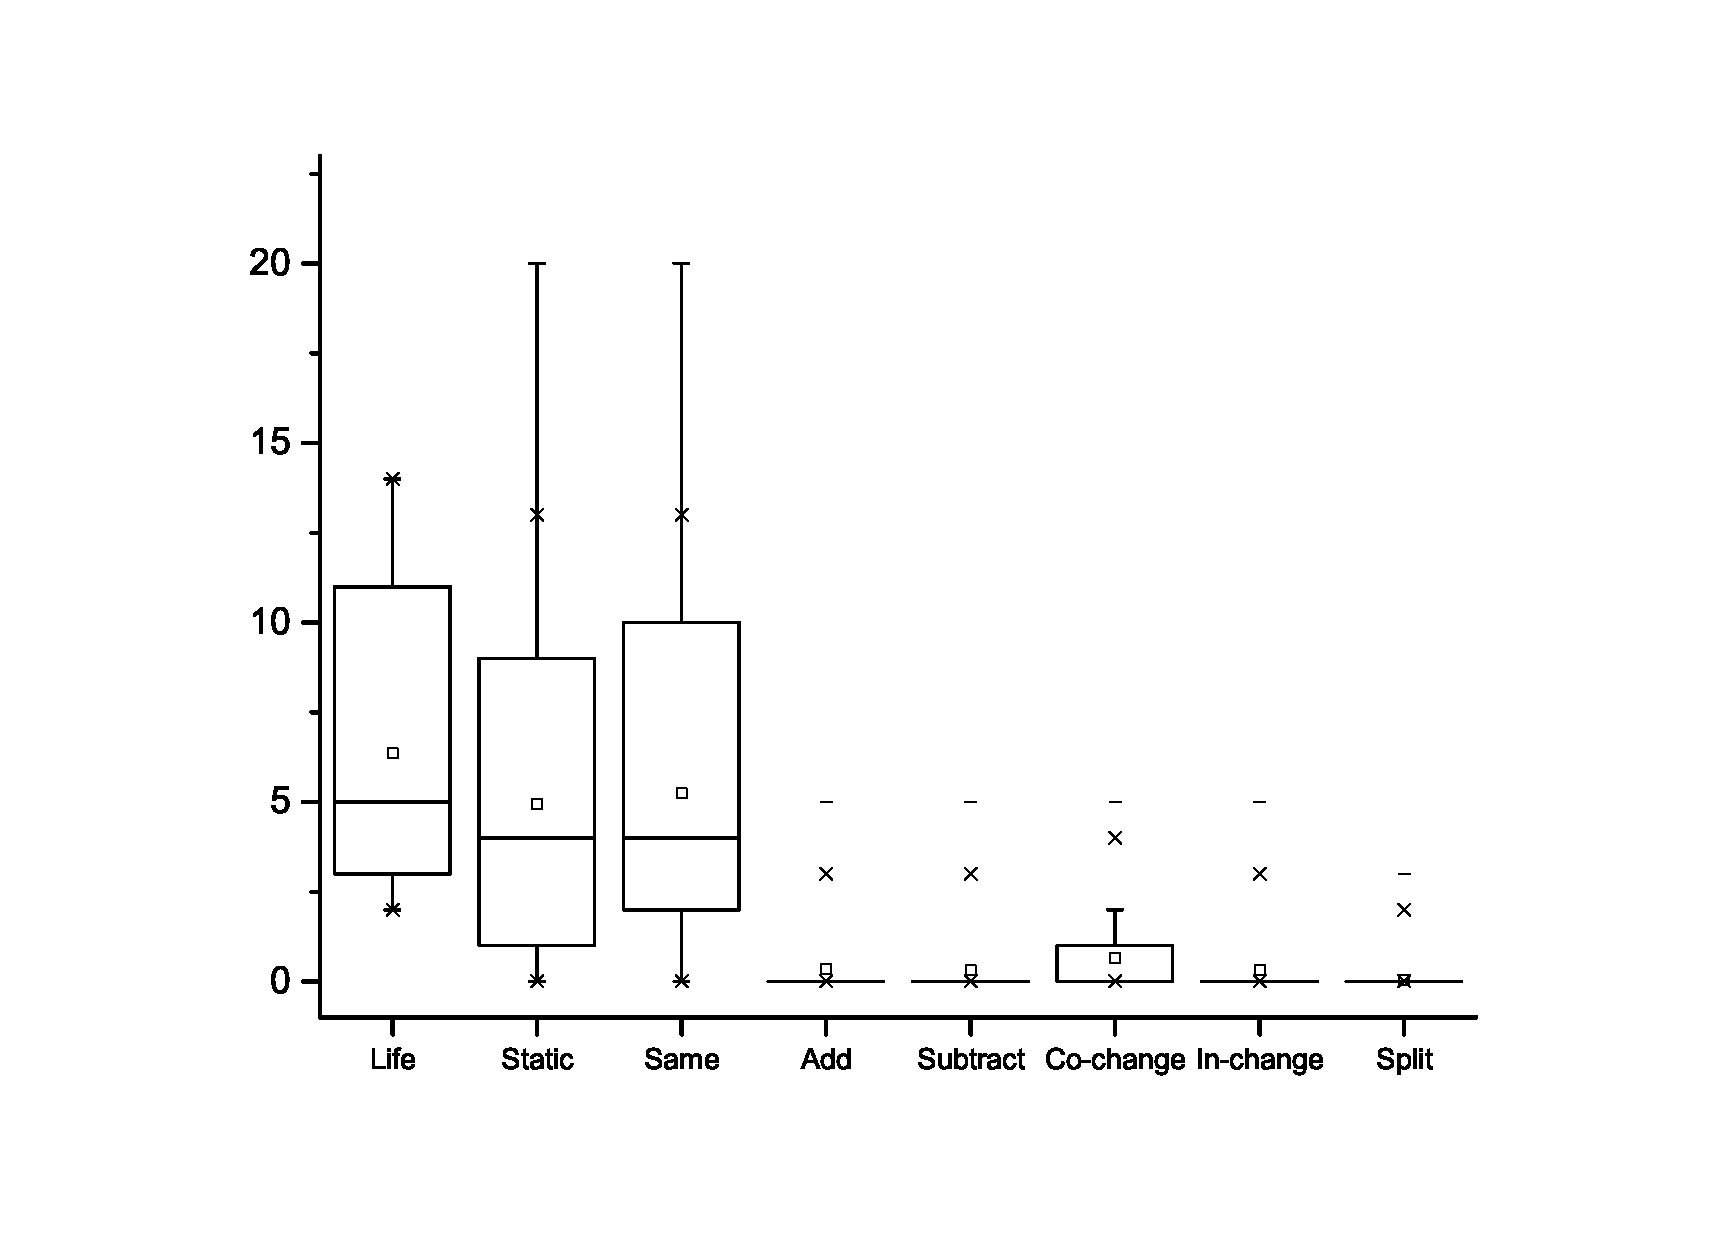
\includegraphics[width=0.8\textwidth]{cgestargo.eps}}}
\subfigure{\label{cgestjedit}}
\addtocounter{subfigure}{-2}
\subfigure[The statistics of clone genealogy evolution for jEdit]
{\subfigure[jEdit中克隆家系的演化模式统计]{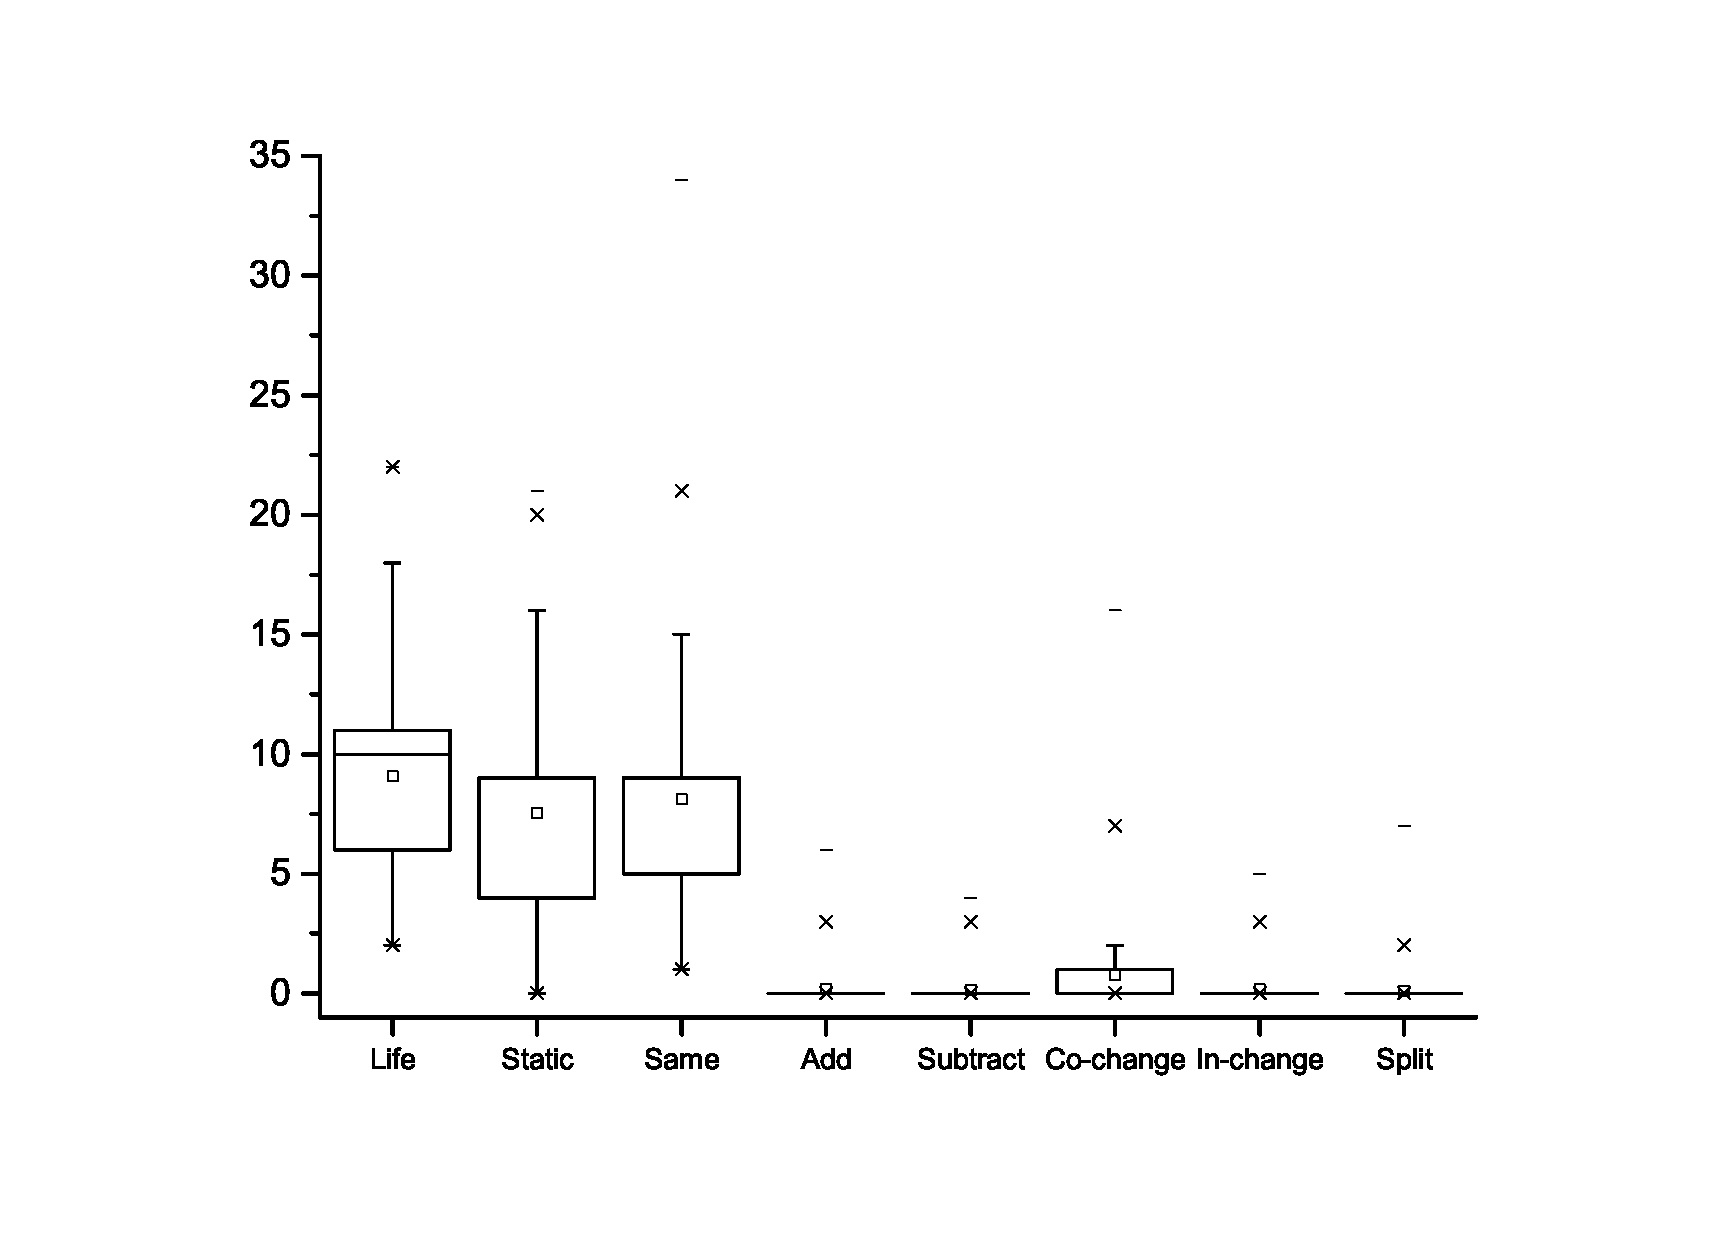
\includegraphics[width=0.8\textwidth]{cgestjedit.eps}}}
\bicaption[cgestas]{}{克隆家系的演化模式统计}
{Fig.$\!$}{The statistics of clone genealogy evolution}
\vspace{-1em}
\end{figure}
 
\BiSubsubsection{克隆家系聚类分析实验}
{Clone Genealogy Experiment of Clustering} 

使用X-means对系统中克隆家系实体的演化情况进行聚类分析(即克隆寿命和克隆演化模式数量),进而挖掘更多的克隆演化特征,结果如表~\ref{cgecluargouml}和~\ref{cgeclujedit}~所示。

表中定义了一个 “Death”的特殊变量,并用其标识实验所收集的克隆家系是否已经死亡。表中“Death”列表示已经死亡的克隆家系的数量,从表中的“Cluster”列和“Death”列中可以发现,本节所收集的克隆家系是完整的,即大部分的克隆家系仍在演化中并没有死亡。同时从表中可以看出,X-means将所有克隆家系可以聚类成4个Cluster:Cluster0-Cluster3。

为了分析克隆家系的演化情况,本节非正式给出“稳定的”和“动态的”的克隆家系。如果一个克隆家系中具有大量的稳定的克隆演化模式,即克隆家系中存在大量的“静态(Stactic)”和“相同(Same)”演化模式,则称克隆家系是 “稳定的”克隆家系(Stable Clone Genealogy)。相反地称一个克隆家系是“动态的”克隆家系(Dynamic Clone Genealogy),即该克隆家系具有相对较多的“Add”,“Subtract”,“ Split”和“Consistent/Inconsistent Change”克隆演化模式。

从图~\ref{cgestas}和表~\ref{cgecluargouml}~和~\ref{cgeclujedit}~中,可以很明显的看出,大多数的克隆家系是“稳定的”克隆家系(Cluster1,2,3),并且克隆家系寿命和“稳定的”克隆模式之间存在较强的正相关关系。另一方面,“动态的”克隆家系(Cluster0)数量十分稀少,并且具有较长的寿命且依然存在于系统中。这表明“动态的”克隆演化模式--特别是一致性变化和不一致性变化-- 通常发生在寿命较长的克隆家系中。因此,软件开发人员应该对动态的克隆家系采取一些必要的措施,因为不一致性的变化可能导致软件缺陷。

对于Cluster3中的克隆家系(表~\ref{cgecluargouml}和~\ref{cgeclujedit}),其寿命较短,并且它们中的大多数已经死亡。但是,这些克隆家系却非常稳定,不存在不一致性变化演化模式。因此可以得出结论:寿命较短的克隆家系比寿命较长的克隆家系更为稳定。这也提醒软件开发人员,不需要关注那些新创建的克隆家系(寿命较短的克隆家系),但随着时间的推移,程序开发人员更应该关注那些依然存在系统中的寿命较长的克隆家系。

综上所述,克隆家系在整个演化过程中大多是稳定的,而较短寿命的克隆家系相比寿命较长的克隆家系更为稳定。 同时,动态的演化模式通常发生在较长寿命的克隆家系中(即使其数量比较稀少),其中一致性变化模式比不一致性变化模式更为频繁。因此,本文建议开发人员应该更加注意寿命较长的克隆家系,并且当克隆代码发生变化时需要考虑同组克隆代码的一致性变化。
 
\begin{table} [htbp]
\bicaption[cgecluargouml]{}{ArgoUML中克隆家系的聚类结果}
{Table$\!$}{Clustering results of clone genealogy for ArgoUML}
\vspace{0.5em}
\centering
\footnotesize
\begin{tabular}{ccccccccccc}
\toprule[1.5pt]
Cluster&Death&Metric&Life&	Static&	Same&	Add	&Subtract&	Consistent&	Inconsistent&	Split\\ 
\midrule[1pt]
Cluster0&\multirow{3}{*}{5}&Mean	&11.854	&9.795	&10.451	&2.232&	2.232&	3.061&	2.293&	0.390\\ 
82&&SD&1.820&2.989&	3.048&	1.046&	1.081&0.851&1.071&	0.843\\ 
(8\%)&&Median	&11&	10&	10&	2&	2&	3&	2	&0\\ 
\hline
Cluster1&\multirow{3}{*}{39}&Mean	&10.192&8.831&9.096	&0.171&0.122	&0.444&0.122&0.005\\ 
385&&SD&	1.680	&1.676&1.703&0.398&	0.328	&0.648&	0.328	&0.102\\ 
(37\%)&&Median	&11	&9	&10	&0&	0&	0&	0	&0\\ 
\hline
Cluster2&\multirow{3}{*}{188}&Mean	&3.294&1.255	&2	&0.471&0.461&1.260	&0.461	&0.010\\
204&&SD&1.228&1.355&1.324&0.639&0.6389&0.440&0.638&0.140\\ 
(20\%)&&Median	&3&	1&	2&	0&	0&	1&	0&	0\\ 
\hline
Cluster3&\multirow{3}{*}{348}&Mean	&2.795	&1.795	&1.795	&0	&0	&0	&0	&0\\ 
365&&SD&1.081	&1.081&1.081&0	&0	&0	&0	&0\\ 
(35\%)&&Median	&3	&2	&2	&0	&0	&0&	0&	0\\ 
\hline
All&\multirow{3}{*}{579}&Mean	&6.359&4.936&5.234&0.333	&0.313&0.655	&0.318&0.035\\ 
1036&&SD&4.025	&4.022	&4.062	&0.750	&0.745&0.974&0.757&0.272\\ 
(100\%)&&Median&	5&	4&	4&	0&	0&	0&	0&	0\\
\bottomrule[1.5pt]
\end{tabular}
\end{table} 

\begin{table} [htbp]
\bicaption[cgeclujedit]{}{jEdit中克隆家系的聚类结果}
{Table$\!$}{Clustering results of clone genealogy for jEdit}
\vspace{0.5em}
\centering
\footnotesize
\begin{tabular}{ccccccccccc}
\toprule[1.5pt]
Cluster&Death&Metric&Life&	Static&	Same&	Add	&Subtract&	Consistent&	Inconsistent&	Split\\
\midrule[1pt]
Cluster0&\multirow{3}{*}{3}&Mean	&19	&15.8	&19.2	&3	&2.3&	6	&2.7&	1.1\\ 
10&&SD&4.830&4.566&	6.426&1.333&	0.949&	4.570&	1.418&2.234\\ 
(4\%)&&Median	&22&	17&	19&	3&	2	&4.5	&2.5&	0\\ 
\hline
Cluster1&\multirow{3}{*}{35}&Mean	&10.952&	9.445&	9.938&	0.075	&0.075	&0.589&	0.082&	0.041\\ 
146&&SD&2.356&2.166&2.358&0.265	&0.313&	1.074&	0.343&	0.285\\ 
(62\%)&&Median&	10&	9&	9	&0&	0	&0	&0&	0\\ 
\hline
Cluster2&\multirow{3}{*}{24}&Mean	&6.571&	4.75&	5.607&	0.071&	0.071&	0.857&	0.071&	0.071\\ 
28&&SD&1.168&	1.143&1.227&0.262&0.262&0.970&0.262&0.378\\ 
(12\%)&&Median	&7	&5	&6&	0	&0	&1&	0&	0\\ \hline
Cluster3&\multirow{3}{*}{48}&Mean	&3.340&	2.132&	2.302&	0.038&	0	&0.208&	0	&0\\ 
53&&SD&	0.732&0.921&0.723&	0.192&	0&	0.454&0	&0\\ 
(22\%)&&Median	&3&	2&	2	&0&	0&	0	&0&	0\\ \hline
All&\multirow{3}{*}{110}&Mean	&9.072&7.523&	8.110&0.190&	0.152&	0.764	&0.173&	0.080\\ 
237&&SD&4.366&	4.079&4.569&0.690&	0.554&	1.706&0.664	&0.550\\ 
(100\%)&&Median	&10	&9	&9	&0	&0	&0	&0	&0\\
\bottomrule[1.5pt]
\end{tabular}
\end{table} 
 
%%%%以下是未保留小数的表格
%%%begin{table}[htbp]
%%%\bicaption[cggcluargouml]{}{ArgoUML中克隆家系的聚类结果}
%%%{Table$\!$}{Clone Genealogy Clustering Results of ArgoUML}
%%%\vspace{0.5em}
%%%\centering\wuhao
%%%\begin{tabular}{ccccccccccc}
%%%\toprule[1.5pt]
%%% &Death&&Genealogy Life&	Static&	Same&	Add	&Subtract&	Consistent&	Inconsistent&	Split\\ 
%%%\midrule[1pt]
%%%Cluster0&\multirow{3}{*}{5}&Mean	&11.85366	&9.79268	&10.45122	&2.23171&	2.23171&	3.06098&	2.29268&	0.39024\\ \cline{3-11}
%%%82&&Standard Deviation	&1.81979	&2.98861&	3.04758&	1.04585&	1.08068	&0.85125&1.07138&	0.84263\\ \cline{3-11}
%%%(8\%)&&Median	&11&	10&	10&	2&	2&	3&	2	&0\\ \hline
%%%Cluster1&\multirow{3}{*}{39}&Mean	&10.19221	&8.83117	&9.0961	&0.17143	&0.12208	&0.44416	&0.12208	&0.00519\\ \cline{3-11}
%%%385&&Standard Deviation&	1.67998	&1.67552	&1.70282	&0.39754&	0.3278	&0.64761&	0.3278	&0.10193\\ \cline{3-11}
%%%(37\%)&&Median	&11	&9	&10	&0&	0&	0&	0	&0\\ \hline
%%%Cluster2&\multirow{3}{*}{188}&Mean	&3.29412	&1.2549	&2	&0.47059	&0.46078	&1.2598	&0.46078	&0.0098\\ \cline{3-11}
%%%204&&Standard Deviation	&1.22847	&1.35506	&1.32427	&0.63875	&0.63822	&0.43961	&0.63822	&0.14003\\ \cline{3-11}
%%%(20\%)&&Median	&3&	1&	2&	0&	0&	1&	0&	0\\ \hline
%%%Cluster3&\multirow{3}{*}{348}&Mean	&2.79452	&1.79452	&1.79452	&0	&0	&0	&0	&0\\ \cline{3-11}
%%%365&&Standard Deviation	&1.0813	&1.0813	&1.0813	&0	&0	&0	&0	&0\\ \cline{3-11}
%%%(35\%)&&Median	&3	&2	&2	&0	&0	&0&	0&	0\\ \hline
%%%All&\multirow{3}{*}{579}&Mean	&6.35907	&4.93629	&5.23359	&0.33301	&0.31274	&0.65541	&0.31757	&0.03475\\ \cline{3-11}
%%%1036&&Standard Deviation	&4.02533	&4.0219	&4.06154	&0.74995	&0.74514	&0.97405	&0.75663	&0.27231\\ \cline{3-11}
%%%(100\%)&&Median&	5&	4&	4&	0&	0&	0&	0&	0\\ \hline
%%%\bottomrule[1.5pt]
%%%\end{tabular}
%%%\end{table}

%%%\begin{table}[htbp]
%%%\bicaption[cggclujedit]{}{jEdit中克隆家系的聚类结果}
%%%{Table$\!$}{Clone Genealogy Clustering Results of jEdit}
%%%\vspace{0.5em}
%%%\centering\wuhao
%%%\begin{tabular}{ccccccccccc}
%%%\toprule[1.5pt]
%%%&Death&&Genealogy Life&	Static&	Same&	Add	&Subtract&	Consistent&	Inconsistent&	Split\\
%%%\midrule[1pt]
%%%Cluster0&\multirow{3}{*}{3}&Mean	&19	&15.8	&19.2	&3	&2.3&	6	&2.7&	1.1\\ \cline{3-11}
%%%10&&Standard Deviation	&4.83046	&4.56557&	6.42564	&1.33333&	0.94868&	4.57044&	1.41814	&2.23358\\ \cline{3-11}
%%%(4\%)&&Median	&22&	17&	19&	3&	2	&4.5	&2.5&	0\\ \hline
%%%Cluster1&\multirow{3}{*}{35}&Mean	&10.95205&	9.44521&	9.93836&	0.07534	&0.07534	&0.58904&	0.08219&	0.0411\\ \cline{3-11}
%%%146&&Standard Deviation&2.35572	&2.16566&2.35832	&0.26485	&0.31262&	1.07428&	0.34254&	0.28471\\ \cline{3-11}
%%%(62\%)&&Median&	10&	9&	9	&0&	0	&0	&0&	0\\ \hline
%%%Cluster2&\multirow{3}{*}{24}&Mean	&6.57143&	4.75&	5.60714&	0.07143&	0.07143&	0.85714&	0.07143&	0.07143\\ \cline{3-11}
%%%28&&Standard Deviation	&1.16837&	1.14261	&1.22744	&0.26227&0.26227	&0.97046	&0.26227	&0.37796\\ \cline{3-11}
%%%(12\%)&&Median	&7	&5	&6&	0	&0	&1&	0&	0\\ \hline
%%%Cluster3&\multirow{3}{*}{48}&Mean	&3.33962&	2.13208&	2.30189&	0.03774&	0	&0.20755&	0	&0\\ \cline{3-11}
%%%53&&Standard Deviation&	0.73231	&0.92065	&0.72284&	0.19238&	0&	0.45398	&0	&0\\ \cline{3-11}
%%%(22\%)&&Median	&3&	2&	2	&0&	0&	0	&0&	0\\ \hline
%%%All&\multirow{3}{*}{110}&Mean	&9.07173	&7.52321&	8.1097	&0.18987&	0.1519&	0.76371	&0.173&	0.08017\\ \cline{3-11}
%%%237&&Standard Deviation	&4.36559&	4.07926	&4.56922	&0.6903&	0.55438&	1.70588	&0.66354	&0.55033\\ \cline{3-11}
%%%(100\%)&&Median	&10	&9	&9	&0	&0	&0	&0	&0\\ \hline
%%%\bottomrule[1.5pt]
%%%\end{tabular}
%%%\end{table}


%%%\BiSection{讨论和分析}{Discussion}
%% 
%%%我们的方法取决于NiCad和克隆映射算法构建克隆系谱。 我们使用NiCad检测克隆,其结果然后用于映射克隆,以便构建克隆系谱。更精细的克隆检测工具和更精确的克隆映射算法可能提高后续阶段的质量。请注意,我们的方法很大程度上取决于克隆度量的可用性。我们使用一组指标来表示克隆片段,克隆组,克隆系谱。虽然这些指标对我们有很好的影响,但我们希望将来扩展指标的收集,因为新的有趣指标可以暗示克隆与其进化之间可能存在的新关系。
%%
%%%在将来,我们还可以对具有更多克隆度量的不同软件进行更多的实验。我们相信,我们提出了一些更有意义的结论,以帮助克隆分析和克隆维护。我们还可以对克隆特征进行一些进一步的工作。我们认为克隆特征应该在系统维护期间的克隆分析中使用。例如,我们可以从软件中识别一些特殊的克隆,并且我们打算将其链接到克隆有害性。

\newpage

\BiSection{本章小结}
{Summary of  this Chapter}
 
为挖掘克隆代码及其演化过程的克隆代码演化特征,本章提出一个克隆代码演化特征挖掘方法。本章方法可以分析多版本软件的演化情况,使用聚类分析(X-means)的方法挖掘和分析克隆代码演化特征,帮助程序开发人员理解克隆代码。从克隆片段、克隆组和克隆家系实体三个不同角度,分析和表示克隆代码及其演化情况,并提取相应属性值生成克隆演化特征分析的聚类向量。克隆片段角度重点关注克隆代码的实际变化情况,克隆组角度关注克隆组在相邻两个版本的演化情况,克隆家系则提供了系统中全部克隆代码演化的全局视角。在ArgoUML和jEdit两个软件系统上的实验结果表明:克隆代码在其演化过程中通常是非常稳定的,不会频繁的发生变化。同时,在其演化过程中,仍然存在相当数量的发生变化的克隆代码,需要引起开发人员的关注。由于发生变化的克隆中,一致性变化的数量多于不一致性变化,因此建议开发人员应在修改克隆代码片段时需要考虑克隆代码的一致性问题。本章所挖掘的克隆演化特征,不仅可以帮助开发人员更好地理解克隆,提高系统的可理解性;还可以提供一些建议指导开发人员维护系统中克隆代码,为本文后续的克隆代码一致性维护研究奠定了基础。

%本文的创新点如下:
%\begin{itemize}
%\item 
%本文提出了一个框架分析克隆代码的演化特征,可以帮助程序维护人员维护和管理克隆代码。
%\item 
%本文从三个不同的角度视为将克隆代码一种数据进行分析:克隆片段、克隆组和克隆家系,并提取了相应的度量值表示克隆代码。
%\item 
%本文在两个开源系统上进行了实证研究并获得了相关的克隆演化特征,可以帮助理解和维护克隆代码。
%\end{itemize}
% !Mode:: "TeX:UTF-8" 

\BiChapter{克隆代码创建一致性维护需求预测方法}
{Predicting Clone Creating Consistency-Requirement at Copy-and-Paste Time}

\BiSection{引言}
{Introduction}

在软件开发过程中,程序开发人员会通过复制和粘贴操作复用软件中的既有代码,从而向系统中引入新的克隆代码。新产生的克隆代码在随着软件系统的演化过程中,可能会发生一致性变化而导致软件的额外维护代价。遗忘该一致性变化还会引入与之相关的克隆一致性违背缺陷,从而将进一步增大系统的维护代价。在克隆代码创建时(复制粘贴操作发生时),预测在其演化过程中是否会发生一致性变化,可以有助于降低软件的维护代价。因此,如何在克隆代码创建时预测克隆代码的一致性变化是一个值得研究的问题,可以帮助提高软件质量和可维护性。

鉴于此,本章在定义克隆代码创建时的一致性变化和一致性维护需求的基础上,在克隆代码创建时(复制和粘贴时),使用机器学习方法预测克隆代码的一致性维护需求。首先,通过构建软件系统的克隆家系,收集系统中所有的克隆创建实例(复制粘贴操作),并识别克隆创建实例中被复制和粘贴的克隆代码。然后,提取代码属性和上下文属性表示该创建的克隆代码。最后,使用机器学习方法训练预测模型,并在克隆代码创建时预测其一致性维护需求。在四个开源软件系统上对本章方法进行了评估,实验结果表明本章方法可以高效地预测克隆代码创建一致性维护需求,预测结果的F值在79.4\% - 95.7\%之间,精确率和召回率分别介于79.3\% - 95.8\%和79.4\% - 95.8\%之间。本章所提出的预测方法从规避克隆代码产生的角度降低克隆代码的维护代价,提高了预测的准确率和召回率。

\BiSection{克隆代码额外维护代价的相关研究}
{Related Work for Code Clone of Extra Maintenance}

\BiSubsection{克隆代码的维护代价问题}
{The Problem of Maintenance Cost for Code Clones}
\label{lab-cloningexamples}

研究表明,复制粘贴操作是导致克隆代码产生的主要原因,但是所引入的克隆代码可能会导致额外的软件维护代价。图~\ref{creatingexamplea}~是会导致额外维护代价的克隆代码。开发人员复制了23行的代码片段(Clone Fragment 1),然后粘贴至其它地方(Clone Fragment 2),由此操作引入了克隆代码。在其随着软件系统演化的第2、12、32和33个月,这两个克隆代码片段发生了如下4次修改:(1) 开发人员修改了变量{cockpitServers, cockPorts}和{collectionDirs}(图中Line 2、4、6),将其重命名为其它的变量(如{cockpitServers}变为{m\_cockpitServers})。由于这两个代码片段存在于同一个方法中,并且访问了局部变量,因此被复制的代码片段也发生了相应的变化。(2)开发人员在Line 3后插入了一个函数调用{Config.GetParameter}获取额外的配置信息{m\_cockpitEnvs}。(3)为了遵守新的命名规则,开发人员对Clone Fragment 1的变量{PPE}新增加前缀{StaticRank3},并且对Clone Fragment 2的变量{ PROD}做了相同的操作。(4)开发人员将Line 21的{LogLevel.Warning}更改为{LogLevel.Error}。上述操作要求开发人员同时修改两个克隆代码片段,从而会引发克隆代码的额外维护代价。

\begin{figure}[htbp]
\centering
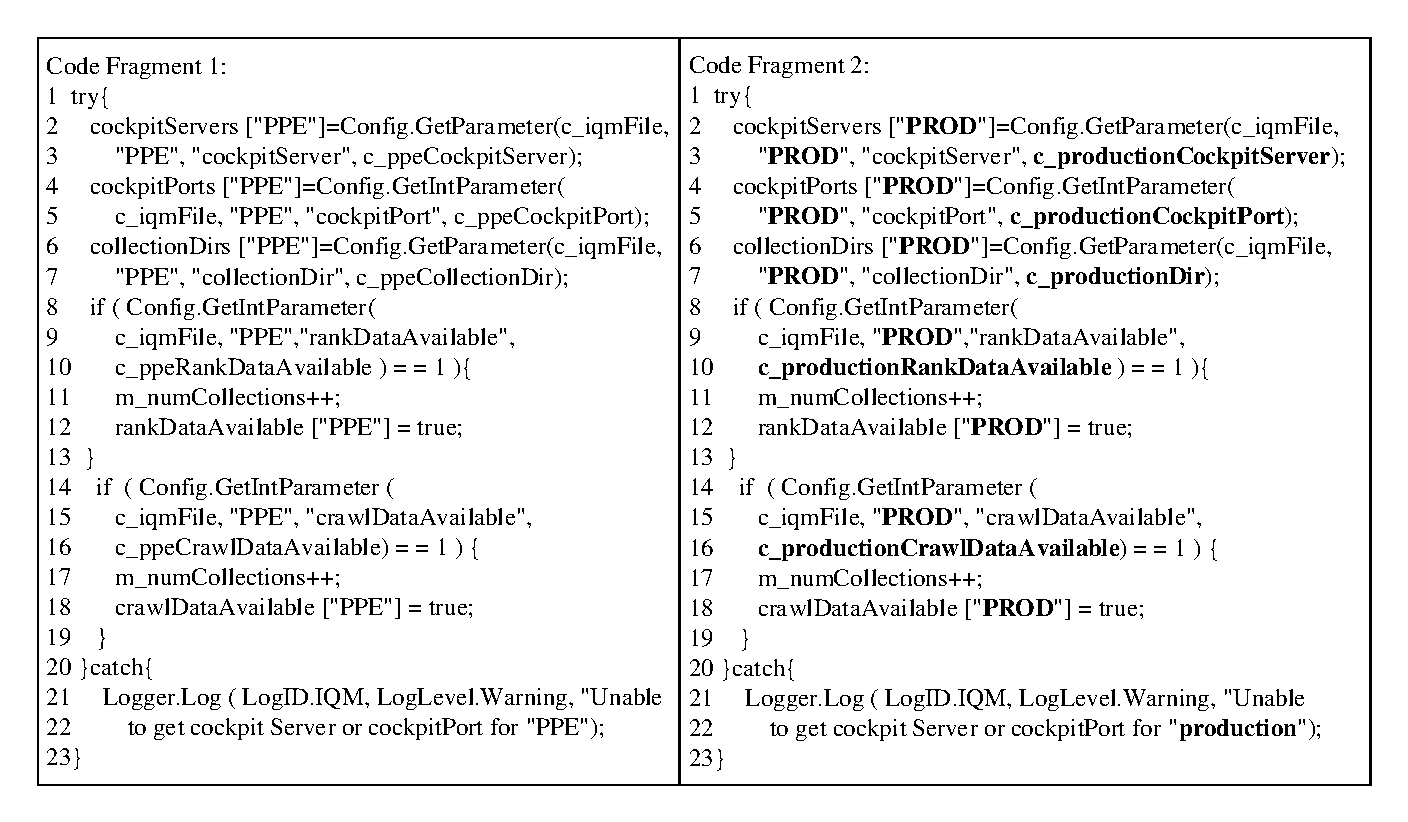
\includegraphics[width = 1.0\textwidth]{creatinga.pdf}
\bicaption[creatingexamplea]{}{会导致额外维护代价的克隆代码\cite{wang2014predicting}}
{Fig.$\!$}{An example for code fragments that resulting extra maintenance cost}
\vspace{-1em}
\end{figure}


但是,并非所有的克隆代码都会导致额外的软件维护代价,图~\ref{creatingexampleb}~是不会导致额外维护代价的克隆代码。开发人员复制一段代码片段,并将其粘贴至其它位置。在引入此克隆代码后,克隆代码一直安静的存在于系统中长达三年的时间,直到包含克隆代码的功能模块被移除。因此,对于此类复制粘贴所导致的克隆代码,并不会引发额外的维护代价。

\begin{figure}[htbp]
\centering
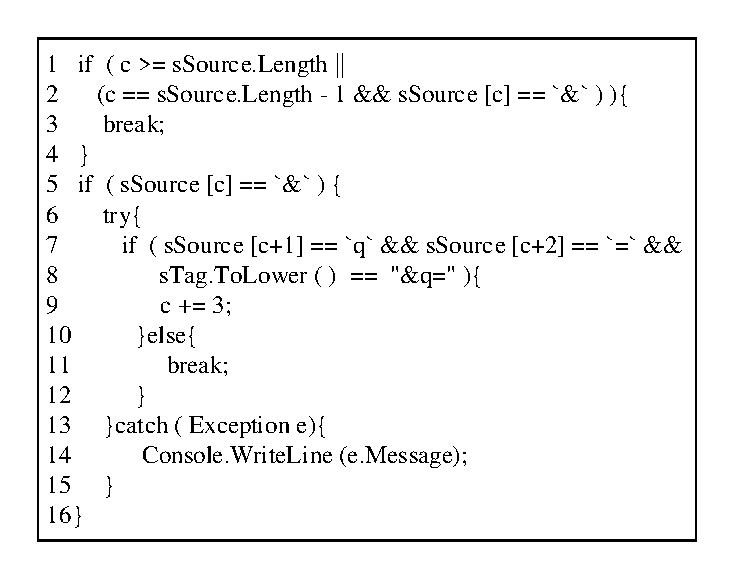
\includegraphics[width = 0.6\textwidth]{creatingb.pdf}
\bicaption[creatingexampleb]{}{不会导致额外维护代价的克隆代码\cite{wang2014predicting}}
{Fig.$\!$}{An example for code fragments that not resulting extra maintenance cost}
\vspace{-1em}
\end{figure}

\BiSubsection{现有方法存在的问题}
{Problems in Current Research}

在软件开发过程中,通过复制粘贴操作复用既有代码已经成为一种常见的软件开发手段\cite{koschke2007survey}。复用既有代码可以减少软件开发时间、提高软件开发效率,但同时也会向软件系统中引入大量的克隆代码。复制和粘贴导致的克隆代码可能引发额外的维护代价,如图~\ref{creatingexamplea}~所示。

针对克隆代码的维护代价问题,当前最主流的解决方式是使用重构的方法消除系统中的克隆代码。拟通过重构的手段消除克隆代码,进而避免克隆代码维护代价。目前的重构研究主要集中在可重构分析\cite{lin2014detecting,mende2009evaluation,schulze2008towards,choi2011extracting}、重构调度\cite{mandal2014automatic,lee2011automated,zibran2011constraint}、重构方法\cite{higo2008metric,krishnan2014unification,barbosa2013removing,ettinger2017efficient}等方面(见本文第~\ref{ref-clonerefactoring}~节克隆代码重构)。由于重构的代价较大,仅有少数的克隆代码适合于重构,因此无法解决克隆代码所导致的额外维护代价问题。

此外,为了有效地管理和维护克隆代码,研究人员也对克隆代码进行跟踪,如跟踪新产生的克隆代码。由于复制粘贴操作是导致克隆产生的最主要原因,因此通过监测程序员的复制粘贴操作可以跟踪克隆代码的产生。例如,许多克隆跟踪工具CLONEBOARD\cite{de2009managing}、CnP\cite{hou2009cnp}、CPC\cite{weckerle2008cpc}、CReN\cite{jablonski2007cren}、CSeR\cite{jacob2010actively}等。但是,对新产生的克隆代码,上述方法并没有进行是否会导致额外维护代价的判断,而是将所有的克隆代码全部引入系统中。因此,也无法帮助降低克隆代码的额外维护代价。

目前,对克隆代码研究无法有效地降低克隆代码的维护代价,依然存在以下两点不足:

(1)现有的克隆代码维护方法主要采用先检测后重构的方法,目标是消除克隆代码,而不是规避克隆代码的产生。这种基于重构的克隆代码维护方法不利于实现边开发边维护克隆代码,不能从源头上规避克隆代码的产生进而降低软件维护代价,而且重构本身的代价也很高,并非所有的克隆代码都适合重构,重构无法从根本上解决克隆代码的维护问题。

(2)在现有的克隆维护中的克隆代码跟踪研究中,通过跟踪复制粘贴操作跟踪克隆代码的产生,但是并未对复制粘贴操作加以控制,对这种操作是否会导致额外的维护代价缺少必要分析和判断。

综上所述,由于开发人员的复制粘贴操作会向系统中引入克隆代码,而克隆代码的一致性变化会导致额外的维护代价,这会降低软件系统的质量和可维护性。因此,结合软件开发过程,在克隆代码创建时(复制和粘贴操作发生时),预测克隆代码的一致性维护需求是一个值得研究的问题,可以帮助规避会引入额外维护代价的克隆代码,从而降低软件的维护代价,提高软件质量和可维护性。具体来说,通过规避会导致额外维护代价的克隆代码产生,可以降低克隆代码的额外维护代价;通过允许不会导致额外维护代价的克隆代码的产生,可以提高软件开发效率。

\BiSubsection{本文的解决思路}
{The Proposed Method}

为了在克隆代码创建时避免其演化过程中可能导致的额外维护代价,本章将解决克隆一致性需求维护预测问题。在克隆代码演化的基础上,结合克隆代码一致性变化所导致的额外维护代价,给出了一种克隆代码创建时的一致性变化以及一致性维护需求的定义。定义不仅可以描述克隆代码所导致的维护代价,还将问题转化为一个可以使用机器学习方法解决的分类问题。然后,本文在Wang\cite{wang2014predicting}等人的研究基础上,改进了用于描述克隆代码的特征属性。舍弃了与复制粘贴操作关联性不强的历史属性,并进一步扩展了代码属性和上下文属性,可以更为细致地表示新创建的被复制和被粘贴的克隆代码。最后,使用五种不同的机器学习方法预测克隆代码创建一致性维护需求。本章方法可以帮助程序开发人员降低克隆代码的一致性维护代价,提高软件的质量和可维护性。

本章的克隆代码创建一致性维护需求预测方法如图~\ref{framwork3}所示。从图中可以看出,该方法可以划分为三个阶段,复制和粘贴操作(克隆创建实例)收集阶段、特征提取阶段和一致性维护需求预测阶段。收集阶段旨在收集系统中全部的复制和粘贴操作,将其用于使用机器学习方法中来训练预测模型。使用NiCad来检测软件版本中的所有克隆,并通过在相邻版本的克隆组之间进行映射来构建克隆家系,用于识别克隆创建实例。首先通过构建系统的克隆家系,然后,将第一次出现在系统的克隆代码标记为由复制和粘贴操作导致的克隆创建实例。最后,通过遍历系统全部克隆家系的根节点,可以收集系统所有的克隆创建实例。

由于实际的克隆创建实例无法直接应用于机器学习方法中,因此在特征提取阶段中将提取相应的属性特征表示克隆创建实例。分别提取了代码属性表示被复制的克隆代码,提取上下文属性表示被粘贴的克隆代码。

在预测步骤中,使用属性化的克隆创建实例构建和训练机器学习模型,并使用其预测克隆一致性维护需求。根据预测结果提醒程序开发人员采取进一步的操作。如果该复制和粘贴操作会导致一致性变化,程序开发人员可以据此拒绝此被复制粘贴的克隆代码,从而避免额外的维护代价。如果该复制粘贴操作不会导致一致性变化(不会引发额外的维护代价),程序开发人员可以放心地复用该克隆代码,从而提高软件开发的效率。

\begin{figure}[htbp]
\centering
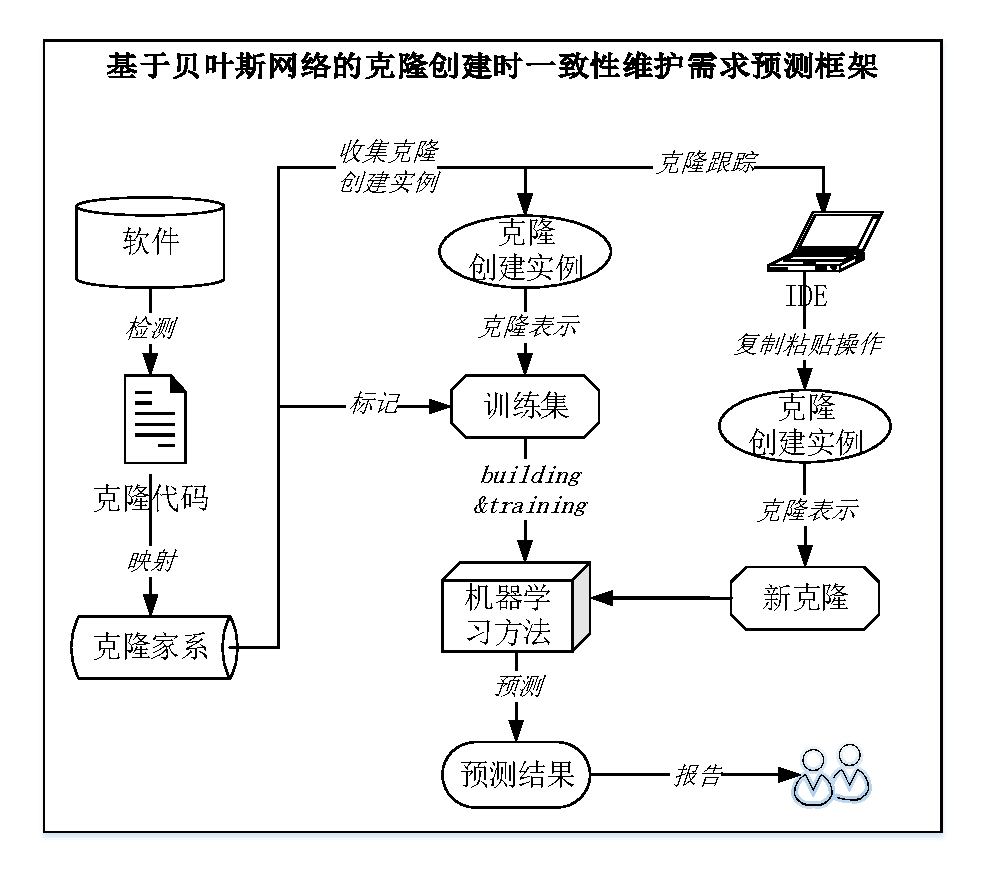
\includegraphics[width = 0.7\textwidth]{framework3.pdf}
\bicaption[framwork3]{}{克隆创建一致性维护需求预测方法}
{Fig.$\!$}{The approach for clone creating consistency prediction}
\vspace{-1em}
\end{figure}

本章在克隆代码创建时预测克隆代码的一致性维护需求,本章将重点分析和讨论如下问题:

(1)在克隆代码创建时(复制和粘贴克隆代码时),结合其可能导致的额外维护代价,如何描述和定义其演化中的一致性变化与一致性维护需求?

(2)对于克隆创建实例(复制和粘贴操作导致的克隆代码),如何进一步深入的描述和表示创建实例中的被复制的克隆代码和被粘贴的克隆代码?

(3)在预测克隆创建一致性维护需求时,如何结合软件开发过程,帮助程序开发人员避免额外的维护代价?

\BiSection{克隆代码创建时一致性维护需求的定义}
{The Definitions for Clone Creating Consistency-Requirement}

如图~\ref{creatingexamplea}~所示,克隆代码的演化过程中,克隆代码可能会发生一致性变化,从而引发额外的维护代价。为了描述克隆代码所发生的变化,本文在第2章中给出了克隆代码的一致性变化模式,见定义\ref{def-evolutionpattern}。但是,
第2章所定义的克隆代码的一致性变化模式过于严格,无法直接用于描述克隆代码可能引发的额外维护代价。

在第2章的定义中,要求克隆组的所有克隆代码片段都要发生相同的变化,才称之为一致性变化。然而,本章的目标是避免克隆代码所导致额外的维护代价,当克隆组内的两个克隆代码同时发生变化时,同样会导致软件的额外维护代价。因此,在向系统中引入新的克隆代码时(克隆代码创建时),本章仅要求至少两个克隆代码片段同时发生变化。

因此,针对克隆代码所导致的额外维护代价问题,将克隆代码的一致性变化模式重新定义如下:

\begin{definition}[克隆创建时一致性变化模式] 
\label{def-creatingpattern}
在软件版本 $j+1$中存在一个克隆组$CG'$ ,假设克隆组内至少存在两个克隆代码片段$CF'_1$ 和 $CF'_2$可以映射到上一版本$j$的克隆组$CG$中,且 $CG$中与之对应的克隆代码片段的 $(CF_1,CF_2)$被分别修改为$(CF'_1,CF'_2)$。如果克隆代码$CF_1$和$CF_2$的变化满足:
\begin{equation}
  \begin{array}[t]{cl}
    \mathit{TextSim}(CF_i, CF'_i) < 1, & \forall i \in \{1,2\}  \\
  \end{array}
\end{equation}
则称克隆组$CG'$具有创建时一致性变化模式(Creating Consistent Change Pattern)。
\end{definition}

在该定义中,克隆代码的变化同样使用$\mathit{TextSim}(CF_i, CF'_i)= 1 - \mathit{UPI}(CF_i, CF'_i)$描述。其中,UPI(Unique Percentage Items\cite{roy2008nicad})表示两个代码片段之间不同的代码行数占总代码行的比例。

本章定义的克隆组的一致性变化模式,仅要求克隆组内至少两个克隆代码片段被同时修改。对于一个克隆组来讲,组内至少存在两个克隆代码片段。假定要求组内全部的克隆代码片段都同时变化,为一致性变化模式。那么此种情况下的定义过于严格。原因在于:即使组内仅有两个克隆代码片段同时发生变化,即会导致额外的维护代价;而要求组内全部克隆片段全部同时变化,将无法准确的识别两个片段变化所导致的维护代价。

如前文所述,系统中的大部分的克隆代码是由复制和粘贴操作所导致的。并且使用克隆家系还可以描述克隆代码的演化过程。因此,在一个克隆家系中,本文认定克隆家系的根节点就是克隆代码创建的时刻,根节点的克隆组是由程序开发人员的复制粘贴操作所创建的克隆代码,称为克隆创建实例。因此,给出克隆创建实例的定义,如下所示:

\begin{definition}[克隆创建实例] 
\label{def-creatinginstance}
软件版本 $j$中的一个克隆组$CG$是克隆创建实例,如果该克隆组$CG$是其克隆家系$CGE$的根节点,且认为该克隆组的克隆代码是由复制粘贴操作引入的。
\end{definition}

给定一个由复制粘贴操作所创建的克隆组,在其演化过程中,可能会发生一致性变化,进而引发额外的维护代价。假设在创建该克隆代码时可以预测其是否可以发生一致性变化,可以避免额外的维护代价。因此,本文将由复制粘贴操作创建的克隆代码,其演化过程中发生的一致性变化称为克隆创建一致性维护需求,定义如下:

\begin{definition}[克隆创建时一致性维护需求] 
 \label{def-creatingrequirement}
给定版本 $j$中一个克隆创建实例$CG$,如果在版本$k$中存在一个克隆组 $CG'$($k>j$)满足以下条件: (1) 在$CG'$中至少存在两个克隆片段在其克隆家系$CGE$中可以映射到克隆实例 $CG$中, (2) $CG'$ 具有“克隆创建时一致性变化模式”(Creating Consistent Change Pattern),则称该克隆创建实例$CG$满足克隆创建一致性维护需求(Creating Consistency-Requirement);反之,假如不存在满足上述条件的克隆组$CG'$,则称 该克隆创建实例$CG$不满足克隆一致性维护需求(Creating Consistency-Requirement Free,或Consistency-Free,或Free)。
\end{definition}

根据上面的定义描述,只要克隆代码在其演化过程中,发生过一致性变化模式,即认定其满足克隆一致性维护需求。最终,本章的研究问题可以表述如下:给定一个克隆创建实例$CG$,例如由复制粘贴操作导致的克隆代码,预测该创建实例$CG$是否满足克隆创建的一致性维护需求。克隆创建实例只有两种状态:满足和不满足一致性维护需求。本章克隆创建的克隆一致性需求预测问题可转换为一个典型的分类问题,因此使用机器学习模型解决此分类问题。

\BiSection{复制和粘贴操作的样本获取}
{Collecting Copy-and-Paste Operations}
\label{lab-checkcopied}

根据定义~\ref{def-creatinginstance}~,本文假定克隆家系$CGE$中第一次出现的克隆代码是克隆创建实例,即复制粘贴操作导致的克隆代码。因此,通过检测系统的克隆代码并构建克隆家系,可以收集系统中的复制和粘贴操作。本章将使用NiCad来检测软件版本中的所有克隆。通过在相邻版本的克隆组之间进行映射来构建克隆家系。

算法~\ref{alg-collectioncreating}~给出了收集系统中复制和粘贴操作的步骤。算法中第1 - 3行是为克隆代码生成CRD,并使用CRD映射相邻版本的克隆代码假设一个版本中有$m$个克隆代码,生成CRD所需时间为$O(m)$,$n$个版本所需时间为$O(m*n)$。映射克隆相邻版本的克隆代码时间复杂度为$O(m)$。算法的第4行为根据映射结果生成系统的克隆家系。第5 - 8行,先根据克隆创建实例定义,通过遍历克隆家系收集系统复制和粘贴操作。然后,根据克隆演化模式定义,识别克隆演化模式,并标记其一致性维护需求。最后,确认复制粘贴操作中被复制和被粘贴的克隆代码。算法复杂度为$O(n)$。所以,该算法的复杂度为$O(m*n)$。

\vspace{1em}
\begin{minipage}{0.8\textwidth}
\centering
\begin{algorithm}[H]
\AlgoBiCaption{复制粘贴操作收集算法} {Algorithm for collecting copy-and-pasted operations}
\label{alg-collectioncreating}
\KwIn{All source code and code clones from $N$ versions}
\KwOut{All copy-and-paste operations}
\For{$i$=1 to $N$}
{ 
 Generating CRD to represent each code clone{CFs}\;
 Mapping all the $CFs$ and $CGs$ between the adjacent versions {i} and {i+1}\;
}
Generating all clone genealogies $CGEs$ with number $N\_cge$\;
\For{$i$=1 to $N\_cge$}
{ 
 Collecting the clone creating instance from $CGE\_i$ according to Definition~\ref{def-creatinginstance}~\; 
 Identify all clone consistent change pattern in thus two versions according to Definition~\ref{def-creatingpattern}~\;
 Labeling its consistency-requirement according to Definition~\ref{def-creatingrequirement}~; 
 Labeling the copied and pasted code fragments by mapping code clones to the last version\;
}
\Return {All copy-and-paste operations\;}
\end{algorithm}
\end{minipage}
\vspace{1em}

(1)构建系统的克隆家系

首先,下载系统所有版本的源代码,并使用NiCad的默认配置检测每一版本的中Type1-3的克隆代码。然后,通过映射所有相邻版本的克隆代码,构建系统中全部克隆家系。为完成版本间的映射,为每个克隆片段生成一个克隆区域描述符 $CRD$\cite{duala2010clone},使用基于$CRD$的克隆映射算法映射两个连续版本之间的所有克隆片段和克隆组\cite{ci2013new,ci2013newD}。根据克隆映射结果,构建系统的克隆家系。

(2)收集复制粘贴操作并标识一致性维护需求

克隆家系是一个克隆组演化的有向无环图,图中根节点是由复制粘贴操导致的克隆创建实例。因此,根据定义~\ref{def-creatinginstance}~通过遍历克隆家系的根节点,可收集系统中所有的克隆创建实例,即复制和粘贴操作。在收集克隆创建实例的时候,同时根据定义~\ref{def-creatingpattern}~识别克隆一致性变化模式,从而确定克隆创建实例在其未来演化过程所发生的一致性变化。根据定义~\ref{def-creatingrequirement}~,如果克隆创建实例在其演化过程中发生了一致性变化模式(定义~\ref{def-creatingpattern}~),则该实例满足一致性维护需求,否则不满足维护需求。

(3)确认被复制和被粘贴的克隆代码

在收集克隆变化实例后,还需确认该实例中的被复制和被粘贴代码。由于被复制代码会较早地存在软件中,可将创建实例中的克隆代码向上一软件版本中进行映射。假定被复制代码会存在于上一版本中,被粘贴代码不存在上一版本中。根据映射结果,可能会存在两种情况:(a) 其中一个克隆代码可以映射,另一个未映射。认为映射代码为被复制代码,未映射为被粘贴代码。(b) 两者均没有映射。此情况下随机选取一个为被复制代码,另一个未未被粘贴代码。原因是两者互为克隆代码,彼此之间相似,故随机选取一个为被复制代码并不影响预测结果。注意不存在两者均可映射的情况,应在上一版本检测为克隆代码\footnote{大多数克隆组只有两个克隆片段,所以这个决定不会影响我们的克隆预测。对于具有多个克隆片段的克隆组,则随机选取两个作为克隆创建实例。}。

\BiSection{复制粘贴操作的特征描述}
{The Attributes for Copied and Pasted Code Clones}
\label{lab-creatingattribute}

在使用机器学习中分类方法进行分类或者预测时,例如本章预测克隆代码创建的一致性维护需求,需要提前构建和训练机器学习模型。但是,实际的复制粘贴操作无法直接应用于机器学习中。因此,本节将使用相应的属性值表示克隆创建实例。克隆创建实例是由复制粘贴操作所引入的克隆代码片段,因此克隆创建实例包含被复制的克隆代码和被粘贴的克隆代码。本章将提取不同的属性用于描述被复制和被粘贴的克隆代码。%提取代码属性表示被复制的克隆代码,提取上下文属性属性表示被粘贴的克隆代码。

\BiSubsection{属性特征分析}
{The Analysis for Code Clone Attributes}

从本章第\ref{lab-cloningexamples}节所给出的克隆代码例子中,可以观察到与克隆代码一致性变化有关联的一些因素。首先,如果两个克隆代码存在于同一个文件中,那么它们可能会共享一些相同的局部方法和局部变量。对其中一个克隆代码片段的修改可能会引发相似的变化。其次,克隆代码自身的一些语法信息,可能也会影响克隆代码的一致性变化。例如,在对{if}语句的条件判定中,往往隐含着一些配置信息和静态作用域相关的变量。如果两个克隆代码片段也包含相同的配置信息或者变量,则对此类变量的修改可能也会导致一致性的变化。最后,克隆代码之间以及克隆代码与其它模块之间的依赖关系,也可能会对克隆代码的一致性变化产生影响。例如,被粘贴的克隆代码片段只包含了一些库函数调用,该克隆代码片段对其它模块的依赖相对较少。因此该被粘贴的克隆代码片段不太可能受到其它模块变化的影响,也就不太容易引发克隆代码的一致性变化。

在一个克隆创建实例中,往往包含着两个不同类型的克隆代码片段,即被复制的克隆代码片段以及被粘贴的克隆代码片段。对于被复制的克隆代码片段,程序开发人员往往不会对其进行修改。而对被粘贴的克隆代码片段,程序开发人员可能会对其进行一定程度的修改,从而使其适用于被粘贴克隆代码的所在位置的环境。因此,本章从这两个不同的角度,提取不同的属性特征表示克隆代码创建实例。对于被复制的克隆片段,从克隆代码本身的角度进行分析,提取代码属性对其进行描述。而对于被粘贴的克隆代码,其可能会被开发人员修改,从两个克隆代码片段之间的区别与联系的角度进行分析,即提取上下文属性进行描述。

\BiSubsection{被复制克隆代码的属性特征}
{The Attributes for the Copied Code Clone}

在克隆创建实例中,被复制的克隆代码代表系统中最初始的代码片段。因此本章从代码本身的角度去描述被复制克隆代码的特征,即代码属性。代码属性描述克隆代码的词法、语法、函数调用等信息,主要包括克隆代码粒度、Halstead属性、结构属性、调用属性等属性。
%,具体的代码属性如下所示:
%部分代码属性源于Wang的工作,本文在其基础上进行了扩展,新增Halstead度量属性、结构属性等。Halstead属性经常用于软件预测中,是用于描述代码特征的度量。结构属性是从代码的语法结构信息。

\begin{itemize}
\item 
克隆粒度:被复制克隆代码的粒度。使用代码行数表示克隆粒度,代码行数是最基本的表示代码规模的度量。代码规模作为基础度量可以帮助预测程序的特性,如可靠性和易维护性等\cite{ramamoorthy1984software}。通过计算克隆代码的位置信息,即可获取克隆粒度。假定该克隆代码在文件中的起始和结束行分别为:$L_s$和$L_n$,则克隆粒度为:{$L_s - L_n$}。
\item 
Halstead属性:被复制克隆代码的代码复杂度Halstead度量\cite{jones1994software}是由Halstead提出的一种基于程序源代码的度量,该度量可以估计程序复杂程度和程序员编写程序花费时间。Halstead有四个基本的属性值,分别统计了该克隆代码片段中的操作符种类、操作数种类、操作符总量和操作数总量。
\item  
结构属性:被复制克隆代码的语法结构信息。Jiang等人使用代码的结构信息生成特性向量用于检测克隆代码,并取得了较好的效果\cite{jiang2007deckard}。因此,使用克隆代码的结构信息描述克隆代码也具有可行性。本文使用的结构信息是指克隆代码片段中关键语句的统计信息,包含{if\_then、if\_else、switch、while、do、for、this\_or\_super}等语句信息的统计。
\end{itemize}

在克隆代码片段中,代码与其它模块的依赖关系可能会影响到一致性变化。因此,本文将克隆代码的函数调用次数作为属性特征,并将其细分为本地函数调用,库函数调用、其它函数调用和总函数调用等属性。

\begin{itemize}
\item  
总函数调用次数:
被复制克隆代码中所有函数调用的次数统计。
\item  
本地函数调用次数:
被复制的克隆代码中,调用函数与被复制克隆片段在相同类的调用次数统计。
\item  
库函数调用次数:
被复制的克隆代码中,库函数的调用次数统计,包括java库函数的调用、eclipse库函数的调用以及第三方包的函数调用。
\item  
其它调用次数:
被复制的克隆代码中,既不是库函数调用、也不是本地函数调用的其它调用次数统计,如同项目内其它包函数调用或同包内其它类中的函数调用。
\item  
参数访问数量:被复制克隆代码中所有函数的参数访问数量统计。函数的参数个数也是影响软件质量的因素之一。函数的参数个数和函数调用次数类似,同样也能反应出代码间的依赖程度,因此也会影响克隆片段的一致性维护需求。该度量统计了该克隆代码片段中所有的参数访问次数之和。
\end{itemize}

\BiSubsection{被粘贴克隆代码的属性特征}
{The Attributes for Pasted Code Clone}

克隆创建实例中被粘贴的克隆代码,在其被粘贴到其所在的位置后,程序开发人员可能会对其进行修改。为了描述被粘贴的克隆代码与被复制的克隆代码之间的克隆关系,以及它们之间其它的联系。本章提取上下文属性表示被粘贴的克隆代码,上下文属性是克隆创建实例中克隆代码之间的关系属性。上下文属性包括代码相似度、克隆分布、被复制和被粘贴代码之间的一些相似度等。
%部分上下文属性来自Wang的工作,同时本文也进行了扩展,新增代码相似度、参数类型相似度和块信息标识等属性。

\begin{itemize}
\item
代码相似度:被复制与被粘贴的克隆代码之间的相似度。代码片段越相似,它们之间的关系也就越密切,因而未来修改时也就越可能需要一致性修改。假设$(CF_1,CF_2) $是两个克隆代码片段,其相似度为$\mathit{SimText} (CF_1,CF_2) = 1-\mathit{UPI}$。
\item
局部克隆标识:被复制及粘贴的克隆代码片段是否在同一个文件中。存在同一个文件中,其可能会共享一些局部变量等信息,也意味着可能会引发一致性的变化。 若存在同一文件中,则取值为1,反之取值为0。
\item
文件名相似度:被复制和被粘贴克隆代码所在文件的名相似度。在一些项目中,文件名也往往会隐含一些内在的联系,克隆代码所在文件的文件名越相似,则克隆代码之间的依赖关系可能会更紧密。假定两个克隆片段所在的文件名分别为$M_1$和$M_2$,则文件名相似度为$\mathit{Sim}(M_1,M_2)$。其中,$\mathit{Sim}$使用李氏距离\cite{levenshtein1966binary,navarro2001guided}计算(剩余度量中相似度采用相同方法计算)。
\item
文件名相似度标识:当两个克隆代码是局部克隆时,其文件名相似度标识为1,非局部克隆时为0。该属性决定文件名相似度是否起效。
\item
方法名相似度:被复制和被粘贴克隆代码所在方法的方法名相似度,计算方式同文件名相似度。
\end{itemize}

函数中的参数同样可以影响克隆代码的一致性维护需求。在实际开发过程中,根据程序员的习惯,通常他们会将变量命名成具有实际意义的变量,因此参数名的相似度对于函数的相似度有一定的影响。因此,分别计算以下3种不同属性特征表示包含克隆代码的函数的参数特征。
\begin{itemize}
\item
总参数名相似度:
假定被复制和被粘贴克隆代码所在方法为$M$和$N$,计算其参数名相似度之和。假设M和N分别包含m和n个参数,即$(P_1,P_2,…,P_m)$和$(Q_1,Q_2,…,Q_n)$,则总参数名相似度为$\mathit{\sum_{i=1}^m \sum_{j=1}^n (Sim(P_i,Q_j))}$。
\item
最大参数名相似度:
假定被复制和被粘贴克隆代码所在方法为M和N,其最大参数名相似度。假设M和N分别包含m和n个参数,即$(P_1,P_2,…,P_m)$和$(Q_1,Q_2,…,Q_n)$,最大参数名相似度为$\mathit{Max (Sim(P_i,Q_j))}$。
\item 
总参数类型相似度:
被复制和被粘贴克隆代码所在方法分别为$M$和$N$,其参数类型相似度之和。假设$M$和$N$分别包含$m$和$n$个参数,其参数类型分别为$(P_1,P_2,…,P_m)$和$(Q_1,Q_2,…,Q_n)$,总参数类型相似度$\mathit{\sum_{i=1}^m \sum_{j=1}^n (Sim(P_i,Q_j))}$。
\item
块信息标识:
被复制和被粘贴克隆代码的上下文信息是否相同,若相同为$1$,反之为$0$。
\end{itemize}

综上所述,本章使用代码属性和上下文属性表示克隆创建实例。给定一个克隆创建实例,使用一个$n$维向量表示该克隆创建实例,{$Vector$ ={($v_1$,$v_2$,$...$,$v_m$)}},其中$v_i$表示该克隆创建实例的一个特定属性。对于克隆创建实例,本章共提取了共计28维属性特征,因此$m$取值为28。
%

\BiSection{基于机器学习的克隆创建一致性维护需求预测}
{Predicting Clone Creating Consistency-Requirement base on Machine Learning}
\label{lab-machine}

本章将克隆代码创建的一致性维护需求问题,转化成了克隆创建实例的分类问题,即给定一个克隆创建实例,判别其是否满足克隆创建的一致性维护需求。本章使用五种机器学习方法对克隆创建实例进行分类,从而预测克隆一致性维护需求。

在本章的研究中,使用五种不同的机器学习方法,即贝叶斯网络方法(Bayesian Network,简写为BN)\cite{friedman1997bayesian,pearl1985bayesian}、朴素贝叶斯方法(Naive Bayes,简写为NB)\cite{john1995estimating},支持向量机方法(Support Vector Machine,简称为SVM)\cite{platt199912} 、K近邻方法(K-Nearest Neighbors,简写为KNN) \cite{aha1991instance}和决策树方法(Decision Tree,简写为DT)\cite{quinlan2014c4}。

(1)贝叶斯网络方法

贝叶斯网络是一种概率图型,使用已经观察到的事件来预测将来可能发生的事件\cite{friedman1997bayesian}。贝叶斯网络可以表示成一个有向无环图模型,图中的每一个节点表示一个随机事件,图中的边则表示随机事件发生的条件概率。因此, 贝叶斯网络中的全部节点可以视为一组随机变量{$X_{1},X_{2},...,X_{n}$},贝斯网络的边则可以使用随机变量的条件概率表描述(Conditional Probability Distributions, CPD)。

一般而言,贝叶斯网络的节点可以是随机变量,可以是可观察到的变量、属性、未知参数等。连接两个贝叶斯网络节点的边则代表两个随机变量之间是非条件独立的,使用事件的条件概率表示。如果两个节点间没有连接,就称其随机变量彼此间为条件独立。条件概率表(CPT)可以描述贝叶斯网络的节点和边的因果关系。

对克隆代码一致性维护需求预测而言,贝叶斯网络可用来表示克隆创建实例的属性值及其一致性维护需求间的概率关系。克隆创建实例的属性值是贝叶斯网络中的随机事件。给定一个具体的克隆创建实例,可以使用贝叶斯网络计算该实例满足一致性维护需求的概率。

(2)朴素贝叶斯方法

朴素贝叶斯方法和贝叶斯网络类似,是运用贝叶斯定理为基础的简单概率分类器。但与贝叶斯网络不同的是,朴素贝叶斯方法的特征之间是强(朴素)独立的,因此称为朴素贝叶斯,即假定样本每个特征与其他特征都不相关。 

(3)支持向量机方法

支持向量机是另一种常见的机器学习方法,可以应用在分类与回归问题中。支持向量机方法模型将实例表示为空间中的点,并且试图构造一个超平面将不同类的实例(点)间隔开。更正式地来说,支持向量机在高维或无限维空间中构造超平面或超平面集合,可以用于分类问题中。直观来说,分类边界距离最近的训练数据点越远越好,因为这样可以缩小分类器的泛化误差。

以本文的克隆一致性需求分类为例,每一个克隆代码实例会抽象称为高维空间中的一个“点”,空间维数等同于所提取的属性数量。在使用支持向量机分类克隆实例时,将构造一个超平面分割开两种类别的克隆代码实例。

(4)K近邻方法

K近邻方法是一种用于分类和回归的非参数统计方法。K近邻是一种基于实例的学习方法,是局部近似和将所有计算推迟到分类之后的惰性学习。K近邻会推迟对训练数据的建模,直到需要分类样本时才进行。在K近邻分类中,输出是一个分类族群。一个实例的分类是由其邻居的“多数表决”确定的,K个最近邻居(K为正整数,通常较小)中最常见的分类决定了赋予该对象的类别。若K = 1,则该对象的类别直接由最近的一个节点赋予。邻居都取自一组已经正确分类(在回归的情况下,指属性值正确)的对象。

以本文克隆一致性预测为例,每一个克隆代码实例是K近邻中的一个实例。在进行预测时,被预测的克隆实例的类别,将会有其最近的K个邻居进行表决,从而确定其一致性维护需求。

(5)决策树方法

机器学习中另一个常见的分类方法是决策树。决策树是一种简单但是广泛使用的分类器。通过训练数据构建决策树,可以高效的对未知的数据进行分类。决策树代表的是属性值与对象类别之间的一种映射关系。决策树是一个树结构(可以是二叉树或非二叉树)。树中每个节点表示某个属性,而每个分叉路径则代表的某个可能的权重,而每个叶结点则对应从根节点到该叶节点所经历的路径所表示的对象的类别。决策树仅有单一输出,若欲有复数输出,可以建立独立的决策树以处理不同输出。

以克隆一致性需求预测为例,克隆实例所提取的属性即是决策树中的属性,最后的克隆一致性维护需求则是对象的类别。

本章没有对机器学习方法进行改进和研究,模型的构建和训练通过调用现有机器学习工具包WEKA完成。对于每个软件系统,首先,通过收集克隆创建实例并提取相应的属性,用于构建模型训练所需的数据集。然后,调用WEKA中的机器学习算法实现构建和训练克隆一致性预测模型。

\vspace{1em}
\begin{minipage}{0.8\textwidth}
\centering
\begin{algorithm}[H]
\AlgoBiCaption{克隆创建一致性维护需求预测算法} {Algorithm for predicting clone creating consistency}
\label{alg-creatingperdition}
\KwIn{All copy-and-paste operations and source code}
\KwOut{The predictive model}
Initializing the training data set $Sets$ for all the operations\; 
\For{$i$=1 to $M$} 
{ 
Generating all the code attributes for copied code clones\;
Generating all the context attributes for pasted code clones\;
Appending all the attributes as one item to the $Sets$\;
}
Calling WEKA to train the model on training set $Sets$\;
\Return {The predictive model\;}
\end{algorithm}
\end{minipage}
\vspace{1em}

基于机器学习的克隆创建一致性维护需求预测算法如~\ref{alg-creatingperdition}~所示。算法的第1行为初始化训练集。第2 - 5行提取相应的属性组表示克隆创建实例,并生成训练集。最后第6行,使用训练集调用WEKA训练机器学习模型。算法的主要时间消耗在表示克隆创建实例上,其时间复杂度为$O(m)$,其中m为复制粘贴操作的数量。


根据定义~\ref{def-creatingrequirement}~,克隆创建实例有两种不同的状态:
\begin{itemize}
\item 
不需要一致性维护:
若克隆创建实例的预测结果为“不需要”,软件开发人员可以自由的执行克隆创建操作(复制和粘贴),从而提高开发效率。因为该克隆创建实例在未来演化的过程中不会引发一致性变化,也不会导致额外的维护代价。
\item
需要一致性维护:
若克隆创建实例的预测结果为“需要”,软件开发人员需要谨慎的执行克隆创建操作(复制和粘贴)。因为该克隆创建实例在未来演化的过程中可能会引发一致性变化,从而导致系统的额外维护代价。
\end{itemize}

\BiSection{实验结果与分析}
{Experimental Results and Analysis}

\BiSubsection{实验设置}
{Experimental Methodology}

\BiSubsubsection{实验系统}
{Experimental Projects}

本章选取了四个Java开源软件进行实验,其中ArgoUML和 jEdit与第2章中所使用的系统相同。ArgoUML是一个领先的开源UML建模工具,jEdit是程序员开发所使用的编辑器。并增加两个新的软件系统,分别为jFreeChart和Tuxguitar。jFreeChart是一个开源Java库,可以帮助软件开发人员显示高质量的图表。Tuxguitar是一个开源的多轨的吉他指法编辑器,用户可以使用其创建自己的吉他六线谱。

表~\ref{statisticsprojects}~给出了四个实验系统的基本信息情况,表中第2列给出了所分析系统的软件版本数量,第3、4列给出了软件系统的起始版本号和结束版本号。本文选择14个版本的ArgoUML,22版本的jEdit,20个版本的jFreeChart和13个版本的Tuxguitar。

\begin{table}[htbp]
\bicaption [statisticsprojects]{}{四个开源软件实验系统信息}
{Table$\!$}{The information for four open sources experimental projects }
\vspace{0.5em}
\centering 
\wuhao
\begin{tabular}{cccc}
\toprule[1.5pt ]
{实验系统}&{版本数}&Start Version&End Version\\ 
\midrule[1pt]
ArgoUML&14&0.20.0&0.34.0\\ 
jEdit&22&3.0.0&5.0.0\\ 
jFreeChart&20&1.0.0&1.0.19\\ 
Tuxguitar&13&0.7.0&1.3.2\\ 
\bottomrule[1.5pt]
\end{tabular}
\end{table}

表~\ref{copysta}~给出了实验系统的克隆创建实例信息统计。其中,第2列和第3列给出了每个系统克隆创建实例的数量和比例,其中第2列是不需要一致性维护的实例,第3列是需要一致性维护实例。对于需要一致性维护的克隆创建实例,在其演化过程中可能导致一致性变化,因而会增加系统的额外维护代价。

\begin{table}[htbp]
\bicaption[copysta]{}{实验系统的克隆创建实例信息统计}
{Table$\!$}{The statistics for clone creating instances in four projects}
\vspace{0.5em}
\centering
\wuhao
\begin{tabular}{cccc}
\toprule[1.5pt]
~\multirow{2}{*}{实验系统}& \multicolumn{2}{c}{克隆创建实例的数量(比例\%)} & \multirow{2}{*}{总数}\\ 
 \cline{2-3}
~&{不需要维护} &{需要维护} & ~\\
\midrule[1pt]
ArgoUML&	2574(77.1\%)&	766(22.9\%)&	3340\\
jEdit&	560(88.5\%)&	73(11.5\%)&	633\\
jFreeChart&	2013(59.8\%)&	1353(40.2\%)&	3366\\
Tuxguitar&	1016(71.1\%)&	413(28.9\%)&	1429\\
\bottomrule[1.5pt]
\end{tabular}
\end{table}

从表~\ref{copysta}~中可以得出两个发现。第一,软件系统中存在大量的克隆创建实例,数量从633到3366。这说明通过复用既有代码引入克隆代码,已经成为了程序开发人员的一种常用开发手段。第二,软件系统中大部分的克隆创建实例在其演化过程中不满足一致性维护需求(比例从59.8\%到88.5\%)。上述观察到的现象与已有研究的结论相一致\cite{wang2014predicting}\cite{gode2011frequency}。这表明通过复制粘贴所引入的克隆代码,在演化过程中大部分不会发生一致性变化,因此开发人员可以采用这种技术提高软件开发效率。但是,值得注意的是软件系统中依然存在相当数量的需要一致性维护的克隆创建实例,数量从73个到1353个。这警告程序开发人员需要注意克隆代码的一致性维护问题,不可以肆无忌惮的使用该复用技术。

%我们在具有Intel(R)Core(TM)i5-4210M CPU @ 2.60GHz和8G RAM的桌面上运行我们的实验。每个实验花费不到一分钟的模型构建,交叉验证少于5分钟。大多数实验时间花费在数据准备,包括家谱建构和克隆变化实例收集,其范围在5至30分钟之间。然而,我们注意到,在实践中,克隆系谱构建和变更实例收集将逐步执行,随着软件发展到新版本。因此,数据准备的开销将不是实际问题。

为了评估本章所提出的克隆创建一致性维护需求预测方法,本章将实验划分为两个部分,有效性验证实验和使用模式实验:
\begin{itemize}
\item
有效性验证实验:在此实验中,使用五种不同机器学习方法评估本章方法的预测能力。可以帮助程序开发人员选择一个最优的机器学习方法,用于克隆代码创建的一致性维护需求预测。在此实验中,同时预测两种类别的克隆创建实例。
\item
使用模式实验:因为有两种不同类别的克隆创建实例,即需要一致性维护和不需要一致性维护。本节以贝叶斯网络方法为例,详细给出了两种不同状态实例的预测结果,以帮助程序开发人员选择合适的“使用模式”进行克隆创建的一致性维护需求预测。
\end{itemize}

本章提取了两组度量表示克隆创建实例,分别为代码属性和上下文属性。为了评估所提取的属性特征的有效性,本章还将每一个实验进一步划分为全属性实验和属性组实验两个部分:
\begin{itemize}
\item
全属性实验:在此实验中,使用本章所提取的所有属性进行预测实验,以评估本文方法的整体预测能力。
\item
属性组实验:
在此实验中,分别使用两组不同的属性值进行预测实验,以评估所提取的属性值对预测结果的影响程度。
\end{itemize}

\BiSubsubsection{实验评估指标}
{The Metrics for Evaluation }
\label{ref-creatingmetrics}

在机器学习领域中,往往使用混淆矩阵(Confusion Matrix)描述一个机器学习模型的预测能力。混淆矩阵如表~\ref{confusion}~所示。在表中,True Positives(TP)表示被正确地划分为正例的个数,即实际为正例且被分类器划分为正例的实例数。False Positives(FP)表示被错误地划分为正例的个数,即实际为负例但被分类器划分为正例的实例数。False Negatives(FN)表示被错误地划分为负例的个数,即实际为正例但被分类器划分为负例的实例数。True Negatives(TN)表示被正确地划分为负例的个数,即实际为负例且被分类器划分为负例的实例数。  ​

\begin{table}[htbp]
\bicaption[confusion]{}{混淆矩阵示意图}
{Table$\!$}{The Confusion Matrix}
\vspace{0.5em}
\centering
\wuhao
\begin{tabular}{ccc}
\toprule[1.5pt]
~\multirow{2}{*}{真实类别}& \multicolumn{2}{c}{预测类别} ~\\ 
 \cline{2-3}
~&{类别$0$} &{类别$1$}~\\
\midrule[1pt]
类别$0$&True Positive(TP)	&False Negative(FN)\\
类别$1$&False Positive(FP)	&True Negative(TN)\\
\bottomrule[1.5pt]
\end{tabular}
\end{table}

根据混淆矩阵,本章计算精确率(Precision Rate)、召回率(Recall Rate)和F值(F-measure)作为评价模型预测能力的指标。
%%%\begin{itemize}
%%%\item	
%%%推荐率(Recommendation Rate):指的是所推荐的不需要一致性维护的克隆创建实例比例,即预测为不需要一致性维护的克隆创建实例与系统中全部实例的比值。
%%%\item  
%%%精确率(Precision Rate):指所预测的不需要一致性维护复制粘贴实例的精确率,即在预测为不需要一致性维护的复制粘贴实例中,正确预测的实例与所预测实例的比值。
%%%\item  
%%%召回率(Recall Rate):指所推荐的不需要一致性维护的复制粘贴实例的查全率,即预测为不需要一致性维护的复制粘贴实例,与系统中的不需要一致性维护的实例的比值。
%%%\end{itemize}

对于不需要一致性维护的克隆创建实例(类别$0$),其精确率指在预测为不需要一致性维护的复制粘贴实例中,正确预测的实例与所预测实例的比值。Precision可计算如下:
\begin{equation} 
\mbox{\it Precision}~=~{\frac {TP}{TP+FP}}
 \end{equation}
 
召回率指预测为不需要一致性维护的复制粘贴实例,与系统中的不需要一致性维护的实例的比值。Recall可如下计算:
\begin{equation} 
\mbox{\it Recall}~=~{\frac {TP}{TP+FN}}
 \end{equation}

F值是综合精确率和召回率的评价指标,用于评估预测模型的综合能力。F-measure可如下计算:
\begin{equation} 
\mbox{\it F-measure} =2 \times {\frac {\mbox{\it precision} \times \mbox{\it recall} }{ \mbox{\it precision} + \mbox{\it recall} } }
 \end{equation}

%%%\begin{itemize}
%%%\item	
%%%警告率(Warning Rate):
%%%指所警告的需要一致性维护的克隆创建实例,即预测为需要一致性维护的实例与系统中全部实例的比值。这些克隆实例可能会引发一致性变化和额外维护代价。
%%%\item	
%%%精确率(Precision):
%%%指警告为需要一致性维护的克隆创建实例的精确率,即在所预测的需要一致性维护的实例中,正确预测的实例与全部警告实例的比值。
%%%\item	
%%%召回率(Recall):指所警告的需要一致性维护的克隆创建实例的召回率,即预测为需要一致性维护的实例与系统中的需要一致性维护实例的比值。
%%%\end{itemize}

相似地,对于需要一致性维护的克隆创建实例(类别$1$),同样采用精确率(Precision Rate)、召回率(Recall Rate)和F值(F-measure)作为评价指标,计算方式相同。

在本章的一致性维护预测中,将同时预测两种不同的状态的创建实例的预测效果。首先,对于满足和不满足一致性维护需求的克隆创建实例,分别计算其精确率(Precision)、召回率(Recall)和F值(F-measure),用于评估不同类型实例的预测效果。然后,将这两组预测结果根据实际实例的数量进行加权平均,计算平均精确率(Average Precision)、平均召回率(Average Recall)和平均F值(Average F-measure)作为评价指标,计算方式如下所示:

\begin{itemize}

\item
平均精确率:
 该指标评估克隆创建实例的一致性维护需求预测的准确程度,包含了满足和不满足一致性维护需求的实例的预测。首先计算预测中满足一致性维护需求的精确率``$P_1$'',然后计算不满足一致性维护需求的精确率``$P_2$''。最后将这两个值进行加权平均,作为整个模型的精确率。 ``$P_1$'' 是满足一致性维护需求的精确率,并且训练集中所有满足一致性的实例数量为``$N_1$'' ;类似地, ``$P_2$''为不满足一致性维护需求的精确率,且 ``$N_2$''为其数量。平均精确率(Average Precision)计算如下,
\begin{equation} 
\mbox{\it Ave-Precision} ~=~ {\frac {P_1 \times N_1 + P_2 \times N_2}{N_1 + N_2}}
\end{equation}

\item
平均召回率:
该指标评估克隆创建实例的一致性维护预测的查全能力,也包含了满足求和不满足一致性维护需求的预测。分别计算满足和不满足一致性维护需求的实例的召回率,然后对两者进行加权平均。“$R_1$” 是满足一致性维护需求的召回率,并且训练集中所有满足一致性的实例数量为“$N_1$” ;类似地,“$R_2$”为不满足一致性维护需求的召回率,且 “$N_2$”为实例数量。平均召回率(Average Recall)计算如下,
\begin{equation} 
\mbox{\it Ave-Recall} ~=~ {\frac  {R_1 \times N_1 + R_2 \times N_2}{N_1 + N_2}}.
\end{equation}

\item
平均F值:
该指标可以评估所有克隆创建实例的精确率和召回率的平均有效性。首先分别计算满足和不满足一致性维护需求的克隆实例的F值,然后根据实例的数量进行加权平均。为计算本章预测的平均F-measure, ``$F_1$'' 是满足一致性维护需求的克隆实例的F值,且实例的个数为``$N_1$'';``$F_2$'' 是不满足一致性维护需求的克隆实例的F值,且实例的个数为``$N_1$'',则平均F值(Average F-measure) 可计算如下,
\begin{equation} 
\mbox{\it Ave-F-measure} ~=~ {\frac  {F_1 \times N_1 + F_2 \times N_2}{N_1 + N_2}}.
\end{equation}

\end{itemize}

\BiSubsection{有效性验证实验}
{The Effectiveness Experiments for Employed Machine Learning Methods}

在本节的实验中,讨论五种机器学习方法的预测能力,帮助程序开发人员选择合适的机器学习模型。因此,对每一个实验系统使用五种不同的机器学习方法,同时对需要和不需要一致性维护的克隆实例进行预测。

值得注意的是,本章没有对机器学习方法本身做进一步的改进,直接调用WEKA中的机器学习算法进行评估和预测。在使用不同的机器学习方法时,需要对其进行一些基本的参数设置,以构建不同的机器学习模型。本文对相应机器学习方法的参数进行了简单的调整,并获得不错的预测效果。通过进一步的调整机器学习的参数,可以增强所构建机器学习模型的预测能力。

所采用方法的参数设置如下:贝叶斯网络的父节点数设置为$3$,并且设置阈值为$0.5$。 朴素贝叶斯方法只有一个父节点,设置阈值为$0.5$。在支持向量机方法中,选择用Polynomial Kernel作为核函数。决策树方法采用了J48算法作为预测方法,并设置置信度为$0.75$。对K近邻方法,使用Euclidean Distance为距离函数,并且设置邻居个数为$1$。

在本节实验中,使用10-Folds Cross-Validity将数据集分为训练集和测试集,评估不同机器学习方法的预测能力。使用平均精确率(Average Precision)、平均召回率(Average Recall)和平均F值(Average F-measure)作为评价指标。采用五种不同的机器学习方法,预测克隆创建的克隆代码的一致性维护需求,实验分成了两个部分,分别为全属性实验和属性组实验,实验结果分别如表\ref{creatingallavg}~和~\ref{creatingsetavg}~所示。

\BiSubsubsection{全属性实验结果}
{The Results of Clone Creating Consistency for All Attributes}

表~\ref{creatingallavg}~给出了克隆创建实例使用全部属性组进行预测的实验结果。从表中可以看出,五种不同的机器学习方法均可以高效地预测克隆一致性维护需求,精确率从79.3\%到95.8\%,召回率从79.4\%到95.8\% ,F值从79.4\%到95.7\%。具体地,对ArgoUML系统的预测效果最好,F值从88.7\%到95.7\%,jEdit和jFreeChart系统的预测效果次之,F值从84.0到90.3\%,Tuxguitar系统预测效果最差,F值从79.4\%到89.0\%。

机器学习方法对于不同的项目具有不同的预测效果。从表~\ref{creatingallavg}~中可以看出,对ArgoUML系统具有最好的预测效果,对jEdit和jFreeChart的预测效果次之,对Tuxguitar的预测效果最差。对于ArgoUML和Tuxguitar系统来说,这两个系统的数据分布相似,但ArgoUML的预测效果要好于Tuxguitar系统。分析原因是由于ArgoUML系统具有更多的数据,因此所训练的机器学习模型更好。与此同时,jEdit和jFreeChart系统的实验效果发相差不大,但是jEdit的训练集规模是四个系统中最小的。jEdit在训练集较小还可以达到不错的预测效果的原因,可能是由于jEdit系统的样本不平衡。由表\ref{copysta}可以看到,jEdit的数据会向一侧偏移,从而使得预测效果变好。

\begin{table}[htbp]
\bicaption[creatingallavg]{}{克隆创建实例一致性维护需求预测效果}
{Table$\!$}{The effectiveness of clone creating consistency for all attributes}
\vspace{0.5em}
\centering
\wuhao
\begin{tabular}{cccccc}
\toprule[1.5pt]
{指标}&{方法}&{{ArgoUML}}&{{jEdit}}&{{jFreeChart}}&{{Tuxguitar}}\\
\midrule[1pt]
\multirow{5}{*}{平均Precision(\%)}
&{BN}&93.5&88.9&88.3&	83.1\\
&{NB}&	88.6&	87.1&	86.9&	79.3\\
&{SVM}&95.8&	92.4&90.6&88.8\\
&{KNN}&94.0&88.6&90.0&	84.8\\
&{DT}	&93.9&89.8	&89.3&88.9\\
\hline
\multirow{5}{*}{平均Recall(\%)}
&{BN}& 93.6&87.7&	88.2&	83.6\\
&{NB}&88.8&82.0&	86.8&79.4\\
&{SVM}& 95.8&92.1&90.4&88.3\\
&{KNN}&94.0&88.9&	90.0	&84.8\\
&{DT}&94.0	&90.5&	89.2&89.1\\
\hline
\multirow{5}{*}{平均F-measure(\%)}
&{BN}&93.5&88.2&88.1&83.2\\
&{NB}&88.7&84.0&86.7&79.4\\
&{SVM}&95.7&	90.3	&90.3&87.6\\
&{KNN}&94.0&88.7&	90.0	&	84.8\\
&{DT}	&93.9&	90.1	&89.2&89.0\\
\bottomrule[1.5pt]
\end{tabular}
\end{table}

对比不同机器学习方法的有效性,通过对比发现支持向量机在这四个实验系统上具有最佳的预测能力。具体来说,在系统 ArgoUML、jEdit和jFreeChart上有最好的结果。对于Tuxguitar系统来说,决策树具有最好的结果,支持向量机具有第二好的预测结果。与此同时,贝叶斯网络和朴素贝叶斯方法在这四个项目中几乎具有相对较差的预测结果,但是相差并不是特别明显。因此,建议开发人员在需要预测克隆创建实例时优先考虑支持向量机方法,其它的机器学习方法也可以作为选择进行考虑。

%\begin{table}[htbp]
%\bicaption[creatingallfree]{}{克隆创建实例的一致性维护自由的预测效果}
%{Table$\!$}{The Effectiveness of Creating Instances for Consistency-Free}
%\vspace{0.5em}
%\centering
%\wuhao
%\begin{tabular}{cccccc}
%\toprule[1.5pt]
%{\textbf{Metric}}&{\textbf{Method}}&{\textbf{ArgoUML}}&{\textbf{jEdit}}&{\textbf{jFreeChart}}&{\textbf{Tuxguitar}}\\
%\midrule[1pt]
%\multirow{5}{*}{Precision}
%&{BN	}&0.945	&0.943	&0.879	&0.861\\
%&{Natvie	}&0.917	&0.941	&0.863	&0.853\\
%&{SVM}&	0.955	&0.919	&0.889	&0.872\\
%&{KNN}&	0.96	&0.933	&0.905&	0.891\\
%&{J48}&	0.953&	0.936	&0.891	&0.913\\
%\hline
%\multirow{5}{*}{Recall}
%&{BN}&	0.974&	0.916&	0.932	&0.917\\
%&{Natvie	}&0.94&	0.85&	0.927	&0.858\\
%&{SVM}&	0.992	&0.998	&0.959&	0.979\\
%&{KNN}&	0.962&	0.943	&0.93	&0.896\\
%&{J48}&	0.969&	0.959&	0.934&	0.935\\
%\hline
%\multirow{5}{*}{F-measure}
%&{BN}&	0.959	&0.929&	0.905&	0.888\\
%&{Natvie	}&0.928	&0.893	&0.894	&0.856\\
%&{SVM}&	0.973	&0.957&	0.923	&0.923\\
%&{KNN}&	0.961&	0.938	&0.917	&0.893\\
%&{J48}&     0.961&	0.947	&0.912&	0.924\\
%\bottomrule[1.5pt]
%\end{tabular}
%\end{table}

%\begin{table}[htbp]
%\bicaption[creatingallmeeting]{}{克隆创建实例的一致性维护需求的预测效果}{Table$\!$}
%{The Effectiveness of Creating Instances for Meeting Consistency-Requirement}
%\vspace{0.5em}
%\wuhao
%\centering
%\begin{tabular}{cccccc}
%\toprule[1.5pt]
%{\textbf{Metric}}&{\textbf{Method}}&{\textbf{ArgoUML}}&{\textbf{jEdit}}&{\textbf{jFreeChart}}&{\textbf{Tuxguitar}}\\
%\midrule[1pt]
%\multirow{5}{*}{Precision}
%&{BN}&	0.808	&0.575	&0.809	&0.637\\
%&{Natvie}&	0.714	&0.589	&0.78	&0.637\\
%&{SVM}&	0.845	&0.329	&0.823	&0.646\\
%&{KNN}&	0.864	&0.479	&0.854	&0.731\\
%&{J48}&	0.841	&0.493	&0.831	&0.782\\
%\hline
%\multirow{5}{*}{Recall}
%&{BN}&	0.902	&0.472	&0.889	&0.758\\
%&{Natvie}&	0.78	&0.339	&0.878	&0.646\\
%&{SVM}&	0.969	&0.96	&0.931	&0.927\\
%&{KNN}&	0.872	&0.522	&0.892	&0.74\\
%&{J48}&	0.891	&0.61	&0.894	&0.83\\
%\hline
%\multirow{5}{*}{F-measure}
%&{BN}&	0.853	&0.519	&0.847	&0.692\\
%&{Natvie}&	0.746	&0.43	&0.826	&0.641\\
%&{SVM}&	0.902	&0.49	&0.873	&0.762\\
%&{KNN}&	0.902	&0.49	&0.873	&0.762\\
%&{J48}&	0.865	&0.545	&0.861	&0.805\\
%\bottomrule[1.5pt]
%\end{tabular}
%\end{table}

\BiSubsubsection{属性组实验结果}
{The Results of Clone Creating Consistency for Attribute Set}

为探索不同属性组对预测效果的影响,在五个机器学习方法上进行了属性组实验。分别使用代码属性和上下文属性进行预测,实验结果如表~\ref{creatingsetavg}~所示。表中“全部属性”表示使用全部属性组的预测结果,“代码属性”和“上下文属性”分别为仅使用一组属性的实验结果。

\begin{table} [htbp]
\renewcommand\arraystretch{0.9} 
\bicaption[creatingsetavg]{}{克隆创建实例的属性组预测效果}
{Table$\!$}
{The effectiveness of clone creating consistency for attribute sets}
\vspace{0.5em}
\centering
\wuhao
\begin{tabular}{cccccccc}
\toprule[1.5pt]
~{指标}&{实验系统}&{实验组}&{BN}&{NB}&{SVM}&{KNN}&{DT}~\\
\midrule[1pt]
\multirow{12}{*}{平均Precision(\%)}
&~\multirow{3}{*}{ArgoUML}
&全部属性& 93.5    & 88.6  &95.8 & 94.0  & 93.9 \\
& & 代码属性& 91.2    & 86.6  & 92.8 & 91.1 & 90.4 \\
&  & 上下文属性& 91.7    & 87.7  & 94.2 & 93.3 &93.0  \\
\cline{2-8}
&~\multirow{3}{*}{jEdit}
& 全部属性& 88.9    & 87.1  & 92.4 &88.6 & 89.8 \\
&    &代码属性& 88.5    & 86.5  & 92.4 & 90.3 & 88.2 \\
&    &  上下文属性 & 83.0     &83.2  & 90.9 & 87.7 & 87.6 \\
\cline{2-8}
&~\multirow{3}{*}{jFreeChart}
& 全部属性& 88.3    & 86.9  &90.6 &90.0  & 89.3 \\
&  &代码属性 & 80.8    & 75.5  & 81.9 & 80.8 & 80.2 \\
&  & 上下文属性& 90.3    & 87.3  & 90.6 & 89.8 & 89.1 \\
\cline{2-8}
&~\multirow{3}{*}{Tuxguitar} 
&全部属性 & 83.1    & 79.3  & 88.8 & 84.8 & 88.9 \\
&   &代码属性& 81.1    & 74.7  & 83.4 & 80.6 & 80.0   \\
&    &  上下文属性& 84.3    & 82.4  & 87.3 & 86.1 & 88.1 \\
\hline
\multirow{12}{*}{平均Recall(\%)}&
~\multirow{3}{*}{ArgoUML}
&全部属性 & 93.6    & 88.8  & 95.8 & 94.0  & 94.0  \\
&   &代码属性 & 91.4    & 86.8  & 92.9 & 91.2 & 90.5 \\
&   &  上下文属性& 91.9    & 88.0   & 94.3 & 93.4 & 93.1 \\
\cline{2-8}
&~\multirow{3}{*}{jEdit}
& 全部属性& 87.7    & 82.0   & 92.1 & 88.9 & 90.5 \\
&   &代码属性 & 86.9    & 83.6  & 92.1 & 91.2 & 89.6 \\
&   &  上下文属性& 85.2    & 82.6  & 91.8 & 88.5 & 88.9 \\
\cline{2-8}
&~\multirow{3}{*}{jFreeChart} 
 & 全部属性 & 88.2    & 86.8  & 90.4 & 90.0   & 89.2 \\
&  &代码属性 & 80.3    & 75.2  & 80.6 & 80.3 & 79.6 \\
&   &  上下文属性 & 90.3    & 87.3  & 90.4 & 89.8 & 89.0  \\
\cline{2-8}
&~\multirow{3}{*}{Tuxguitar} 
&全部属性 & 83.6    & 79.4  & 88.3 & 84.8 & 89.1 \\
&   &代码属性 & 81.7    & 75.6  & 83.7 & 81.0  & 80.7 \\
&    & 上下文属性& 84.6    & 81.6  & 87.4 & 86.2 & 88.2 \\
\hline
\multirow{12}{*}{平均F-measure(\%)}
&~\multirow{3}{*}{ArgoUML}
& 全部属性 & 93.5    & 88.7  & 95.7 & 94  & 93.9 \\
 &  & 代码属性 & 91.2    & 86.7  & 92.7 & 91.2 & 90.4 \\
 &   &  上下文属性& 91.7    & 87.8  & 94.1 & 93.3 & 93.0  \\
\cline{2-8}
&~\multirow{3}{*}{jEdit} 
& 全部属性 & 88.2    & 84.0   & 90.3 & 88.7 & 90.1 \\
&   &代码属性& 87.6    & 84.8  & 90.3 & 90.5 & 88.7 \\
&   &  上下文属性& 84.0     & 82.9  & 90.7 & 88.1 & 88.1 \\
\cline{2-8}
&~\multirow{3}{*}{jFreeChart} 
&  全部属性& 88.1    & 86.7  & 90.3 & 90.0   & 89.2 \\
&  &代码属性 & 79.7    & 74.1  & 79.7 & 79.6 & 78.8 \\
&   & 上下文属性 & 90.2    & 87.2  & 90.3 & 89.7 & 88.9 \\
\cline{2-8}
&~\multirow{3}{*}{Tuxguitar} 
&全部属性 & 83.2    & 79.4  & 87.6 & 84.8 & 89.0  \\
&  &代码属性& 81.1    & 75.0   & 82.7 & 80.7 & 80.2 \\
&  & 上下文属性& 84.4    & 81.9  & 86.9 & 86.2 & 88.1\\
\bottomrule[1.5pt]
\end{tabular}
\end{table} 

从表中可以看出,所提取的属性特征对克隆代码创建时的一致性维护需求具有积极的作用。首先,属性组实验结果和全部属性组实验结果并没有显著的差异。这表明本章所提取的属性特征不会对克隆创建实例的一致性维护需求预测产生负面影响。其次,效果最差的实验结果往往出现在属性组的实验结果中,即在仅使用代码属性或仅适用上下文属性时。具体来说,对系统ArgoUML、 jFreeChart和 Tuxguitar,其仅使用代码属性进行预测时五种机器学习方法的预测效果最差,而对系统jEdit仅仅使用“上下文” 属性的五种机器学习方法预测效果最差。因此提取的属性特征对预测效果具有积极的作用。

不同的属性特征对不同系统的预测效果也具有不同的作用。首先,对于ArgoUML和jEdit系统来说,使用全部属性的预测效果最好。代码属性和上下文属性在预测中均起到了积极的作用。然后,对系统jFreeChart和Tuxguitar来讲,仅使用上下文属性的预测效果最好,这说明上下文属性对这两个系统起到了更为关键的作用。但是,仅使用代码属性和使用全部属性的预测效果,与其预测的效果相差不大,也具有积极的作用。在预测克隆代码的一致性维护需求时,本文建议保留全部的属性进行预测,因为属性特征可能对未经验证的系统具有积极的作用。

同样对比分析不同机器学习方法之间的预测能力,可以得出与全属性实验相似的结论,即五种机器学习方法的预测能力相差不大,但支持向量机方法具有相对最好的预测能力。因此建议程序开发人员在优先选择支持向量机方法,并在预测时保留所有的属性特征进行预测。


%%%%以下是未经转置的全部实验结果

%%%\begin{sidewaystable} [htbp]
%%%\bicaption[creatingsetavg]{}{克隆创建实例的属性组平均预测效果}
%%%{Table$\!$}
%%%{The average effectiveness of attribute set on creating instances for consistency}
%%%\vspace{0.5em}
%%%\centering
%%%\wuhao
%%%\begin{tabular}{cccccccccccccc}
%%%\toprule[1.5pt]
%%%\multirow{2}{*}{指标}&\multirow{2}{*}{方法}&\multicolumn{3}{c}{ArgoUML}&\multicolumn{3}{c}{jEdit}&\multicolumn{3}{c}{jFreeChart}&\multicolumn{3}{c}{Tuxguitar}\\
%%%\cline{3-14}
%%%&&{全部}&{代码}&{上下文}&{全部}&{代码}&{上下文}&{全部}&{代码}&{上下文}&{全部}&{代码}&{上下文}~\\
%%%\midrule[1pt]
%%%\multirow{5}{*}{平均Percision}
%%%&BN&	0.935&	0.912&	0.917&		0.889&	0.885&	0.83&		0.883&	0.808&	0.903&		0.831&	0.811&	0.843\\
%%%&NB&	0.886&	0.866&	0.877&		0.871&	0.865&	0.832&		0.869&	0.755&	0.873&		0.793&	0.747&	0.824\\
%%%&SVM&	0.958&	0.928&	0.942&		0.924&	0.924&	0.909&		0.906&	0.819&	0.906&		0.888&	0.834&	0.873\\
%%%&KNN&	0.94&	0.911&	0.933&		0.886&	0.903&	0.877&		0.9	&0.808&	0.898&		0.848&	0.806&	0.861\\
%%%&DT&	0.939&	0.904&	0.93&		0.898&	0.882&	0.876&		0.893&	0.802&	0.891&		0.889&	0.8&	0.881\\
%%%\hline
%%%\multirow{5}{*}{平均Recall}
%%%&BN&	0.936&	0.914&	0.919&		0.877&	0.869&	0.852&		0.882&	0.803&	0.903&		0.836&	0.817&	0.846\\
%%%&NB&	0.888&	0.868&	0.88&		0.82&	0.836&	0.826&		0.868&	0.752&	0.873&		0.794&	0.756&	0.816\\
%%%&SVM&	0.958&	0.929&	0.943&		0.921&	0.921&	0.918&		0.904&	0.806&	0.904&		0.883&	0.837&	0.874\\
%%%&KNN&	0.94&	0.912&	0.934&		0.889&	0.912&	0.885&		0.9&	0.803&	0.898&		0.848&	0.81&	0.862\\
%%%&DT&	0.94&	0.905&	0.931&		0.905&	0.896&	0.889&		0.892&	0.796&	0.89&		0.891&	0.807&	0.882\\
%%%\hline
%%%\multirow{5}{*}{平均F-measure}
%%%&BN&	0.935&	0.912&	0.917&		0.882&	0.876&	0.84&		0.881&	0.797&	0.902&		0.832&	0.811&	0.844\\
%%%&NB&	0.887&	0.867&	0.878&		0.84&	0.848&	0.829&		0.867&	0.741&	0.872&		0.794&	0.75&	0.819\\
%%%&SVM&	0.957&	0.927&	0.941&		0.903&	0.903&	0.907&		0.903&	0.797&	0.903&		0.876&	0.827&	0.869\\
%%%&KNN&	0.94&	0.912&	0.933&		0.887&	0.905&	0.881&		0.9&	0.796&	0.897&		0.848&	0.807&	0.862\\
%%%&DT&	0.939&	0.904&	0.93&		0.901&	0.887&	0.881&		0.892&	0.788&	0.889&		0.89&	0.802&	0.881\\
%%%\bottomrule[1.5pt]
%%%\end{tabular}
%%%\end{sidewaystable} 

%%%%以下是两种模式下的实验结果

%\begin{sidewaystable} [htbp]
%\bicaption[creatingsetfree]{}{克隆创建实例的属性组克隆一致性维护自由预测效果}{Table$\!$}
%{The Effectiveness of Attribute Set on Creating Instances for Consistency-Requirement Free}
%\vspace{0.5em}
%\centering
%\wuhao
%\begin{tabular}{cccccccccccccc}
%\toprule[1.5pt]
%\multirow{2}{*}{\textbf{Metric}}&\multirow{2}{*}{\textbf{Method}}&\multicolumn{3}{c}{\textbf{ArgoUML}}&\multicolumn{3}{c}{\textbf{jEdit}}&\multicolumn{3}{c}{\textbf{jFreeChart}}&\multicolumn{3}{c}{\textbf{Tuxguitar}}\\
%\cline{3-14}
%&&\textbf{All}&\textbf{Code}&\textbf{Context}&\textbf{All}&\textbf{Code}&\textbf{Context}&\textbf{All}&\textbf{Code}&\textbf{Context}&\textbf{All}&\textbf{Code}&\textbf{Context}~\\
%\midrule[1pt]
%\multirow{5}{*}{Precision}
%&BN&0.945&	0.932	&0.929&		0.943&	0.942	&0.9	&	&0.879	&0.789	&0.898		&0.861	&0.848	0.88\\
%&NB&0.917	&0.907&	0.913	&	0.941	&0.932&	0.906	&	0.863&	0.744&	0.873	&	0.853&	0.809	&0.89\\
%&SVM&0.955&	0.937	&0.945	&	0.919	&0.919&	0.928&		0.889	&0.779&	0.889	&	0.872	&0.843	&0.877\\
%&KNN&0.96	&0.94	&0.947	&	0.933&	0.934	&0.926	&	0.905&	0.787&	0.896	&	0.891&	0.856&	0.9\\
%&DT&0.953&	0.936	&0.943	&	0.936&	0.923	&0.921&		0.891&	0.778&	0.884	&	0.913	&0.842&	0.907\\
%
%\hline
%\multirow{5}{*}{Recall}
%&BN&0.974	&0.958	&0.969	&	0.916	&0.907&	0.936		&0.932	&0.916	&0.944	&	0.917	&0.905	&0.906\\
%&NB&0.94	&0.924	&0.933&		0.85	&0.879&	0.896		&0.927&	0.892	&0.922	&	0.858	&0.86&	0.845\\
%&SVM&0.992	&0.973&	0.983		&0.998	&0.998&	0.984		&0.959	&0.944	&0.959		&0.979	&0.947	&0.957\\
%&KNN&0.962&	0.946&	0.969	&	0.943	&0.968&	0.945		&0.93&	0.919&	0.937	&	0.896	&0.881&	0.907\\
%&DT&0.969&	0.941	&0.969	&	0.959&	0.963	&0.957	&	0.934	&0.92&	0.939	&	0.935	&0.897	&0.93\\
%\hline
%\multirow{5}{*}{F-measure}
%&BN&0.959&	0.945&	0.949	&	0.929	&0.924&	0.918	&	0.905&	0.848	&0.921	&	0.888&	0.875&	0.893\\
%&NB&0.928&	0.915	&0.923	&0.893	&0.904	&0.901		&0.894&	0.811&	0.897	&	0.856	&0.834	&0.867\\
%&SVM&0.973&	0.955&	0.964	&	0.957&	0.957&	0.955	&	0.923&	0.854	&0.923&		0.923&	0.892&	0.915\\
%&KNN&0.961&	0.943&	0.958	&	0.938	&0.951&	0.935		&0.917	&0.848	&0.916&		0.893&	0.868	&0.903\\
%&DT&0.961&	0.938&	0.956	&	0.947	&0.942&	0.939	&	0.912&	0.843	&0.911&		0.924	&0.868&	0.918\\
%\bottomrule[1.5pt]
%\end{tabular}
%\end{sidewaystable}

%\begin{sidewaystable} [htbp]
%\footnotesize
%\bicaption[sdfj1]{}{克隆创建实例的属性组克隆一致性维护自由预测效果}{Table$\!$}
%{The Effectiveness of Attribute Set for Creating Instances for Meeting Consistency-Requirement}
%\vspace{0.5em}
%\centering
%%\wuhao
%\begin{tabular}{cccccccccccccc}
%\toprule[1.5pt]
%\multirow{2}{*}{\textbf{Metric}}&\multirow{2}{*}{\textbf{Method}}&\multicolumn{3}{c}{\textbf{ArgoUML}}&\multicolumn{3}{c}{\textbf{jEdit}}&\multicolumn{3}{c}{\textbf{jFreeChart}}&\multicolumn{3}{c}{\textbf{Tuxguitar}}\\
%\cline{3-14}
%&&\textbf{All}&\textbf{Code}&\textbf{Context}&\textbf{All}&\textbf{Code}&\textbf{Context}&\textbf{All}&\textbf{Code}&\textbf{Context}&\textbf{All}&\textbf{Code}&\textbf{Context}~\\
%\midrule[1pt]
%\multirow{5}{*}{Precision}
%&BN&	0.902	&0.844	&0.878	&	0.472	&0.447	&0.294	&	0.889	&0.836	&0.91	&	0.758	&0.719	&0.752\\
%&NB&	0.78&	0.728&	0.756	&	0.339	&0.352	&0.266	&	0.878	&0.772	&0.873	&	0.646	&0.593	&0.662\\
%&SVM&	0.969	&0.896	&0.934	&	0.96	&0.96&	0.769	&	0.931	&0.879	&0.931	&	0.927&	0.813	&0.863\\
%&KNN&	0.872	&0.815	&0.888		&0.522	&0.66	&0.5		&0.892	&0.839	&0.9	&	0.74&	0.684	&0.767\\
%&DT&	0.891	&0.799&	0.885	&	0.61	&0.571	&0.529	&	0.894	&0.837&	0.901	&	0.83	&0.697	&0.817\\
%\hline
%\multirow{5}{*}{Recall}
%&BN&	0.808	&0.765&	0.752		&0.575	&0.575	&0.205	&	0.809&	0.636&	0.841	&	0.637&	0.6	&0.697\\
%&NB&	0.714&	0.68	&0.701	&	0.589	&0.507&	0.288		&0.78	&0.542	&0.8	&	0.637	&0.501	&0.743\\
%&SVM&	0.845&	0.779	&0.808	&	0.329	&0.329&	0.411	&	0.823	&0.601&	0.821	&	0.646	&0.567	&0.671\\
%&KNN&	0.864&	0.798	&0.816	&	0.479	&0.479&	0.425	&	0.854&	0.63&	0.838		&0.731	&0.634&	0.751\\
%&DT&	0.841&	0.782	&0.803	&	0.493	&0.384&	0.37	&	0.831&	0.61&	0.817	&	0.782	&0.586	&0.765\\
%\hline
%\multirow{5}{*}{F-measure}
%&BN&	0.853&	0.803&	0.81	&	0.519	&0.503&	0.242	&	0.847&	0.722&	0.874	&	0.692&	0.654&	0.724\\
%&NB&	0.746&	0.703	&0.728		&0.43	&0.416	&0.276	&	0.826	&0.637	&0.835		&0.641	&0.543	&0.7\\
%&SVM&	0.902&	0.834&	0.866&		0.49&	0.49	&0.536	&	0.873&	0.714	&0.873	&	0.762	&0.668&	0.755\\
%&KNN&	0.868&	0.806&	0.85	&	0.5&	0.556	&0.459		&0.873	&0.72	&0.868		&0.736&	0.658	&0.759\\
%&DT&	0.865&	0.79&	0.842	&	0.545&	0.459&	0.435	&	0.861	&0.706&	0.857	&	0.805	&0.637&	0.79\\
%\bottomrule[1.5pt]
%\end{tabular}
%\end{sidewaystable}

\BiSubsection{使用模式实验}
{The Experiments for Two Usage Scenarios}

本节以贝叶斯网络方法为例,分别预测两种不同类别的克隆创建实例,即不满足一致性维护需求的实例(一致性维护自由实验)和满足一致性维护需求的实例(一致性维护实验)。在构建贝叶斯网络时,使用 K2算法建立网络结构,并设置贝叶斯网络的最大父节点个数为$3$,同时使用SimpleEstimator估计贝叶斯网络的条件概率表。在实验时,采用十倍交叉验证(10-Folds Cross-Validity)将克隆创建实例的数据集划分为训练集和测试集,并评估预测模型的预测能力。

使用贝叶斯网络方法进行预测时,会计算克隆创建实例的概率值,表示该实例需要一致性维护需求的概率(在0 - 1之间,数值接近于1表示需要一致性维护,接近于0表示不需要一致性维护)。针对不同的克隆创建实例,设置了不同的阈值进行实验分析。对于不需要一致性维护的实例,其预测值较小(接近于0),当预测值小于等于给定阈值时认定该实例不需要一致性维护。对于需要一致性维护的实例,其贝叶斯网络预测值较大(接近于1),当预测值大于等于该阈值认定该实例需要一致性维护。

\BiSubsubsection{一致性维护自由实验}
{The Experiment for Meeting Clone Creating Consistency-Free}

对不需要一致性维护的克隆创建实例进行预测评估,帮助程序开发人员执行复制和粘贴操作,从而快速安全地进行软件开发。使用三个指标评估预测效果,分别为:推荐率、精确率和召回率。其中,推荐率(Recommendation Rate,RR)指的是所推荐的不需要一致性维护的克隆创建实例比例,即预测为不需要一致性维护的克隆创建实例与系统中全部实例的比值。

%%%\begin{itemize}
%%%\item	
%%%推荐率(Recommendation Rate):指的是所推荐的不需要一致性维护的克隆创建实例比例,即预测为不需要一致性维护的克隆创建实例与系统中全部实例的比值。
%%%\item  
%%%精确率(Precision Rate):指所预测的不需要一致性维护复制粘贴实例的精确率,即在预测为不需要一致性维护的复制粘贴实例中,正确预测的实例与所预测实例的比值。
%%%\item  
%%%召回率(Recall Rate):指所推荐的不需要一致性维护的复制粘贴实例的查全率,即预测为不需要一致性维护的复制粘贴实例,与系统中的不需要一致性维护的实例的比值。
%%%\end{itemize}

(1)全属性实验结果

全属性实验同样使用全部属性在四个实验系统上进行预测,实验结果如图~\ref{creatingallfree}~所示。图中的横坐标表示阈值,设置阈值从0.01到0.50,图中的纵坐标为评价指标的数值大小。

\begin{figure}[h]
\centering
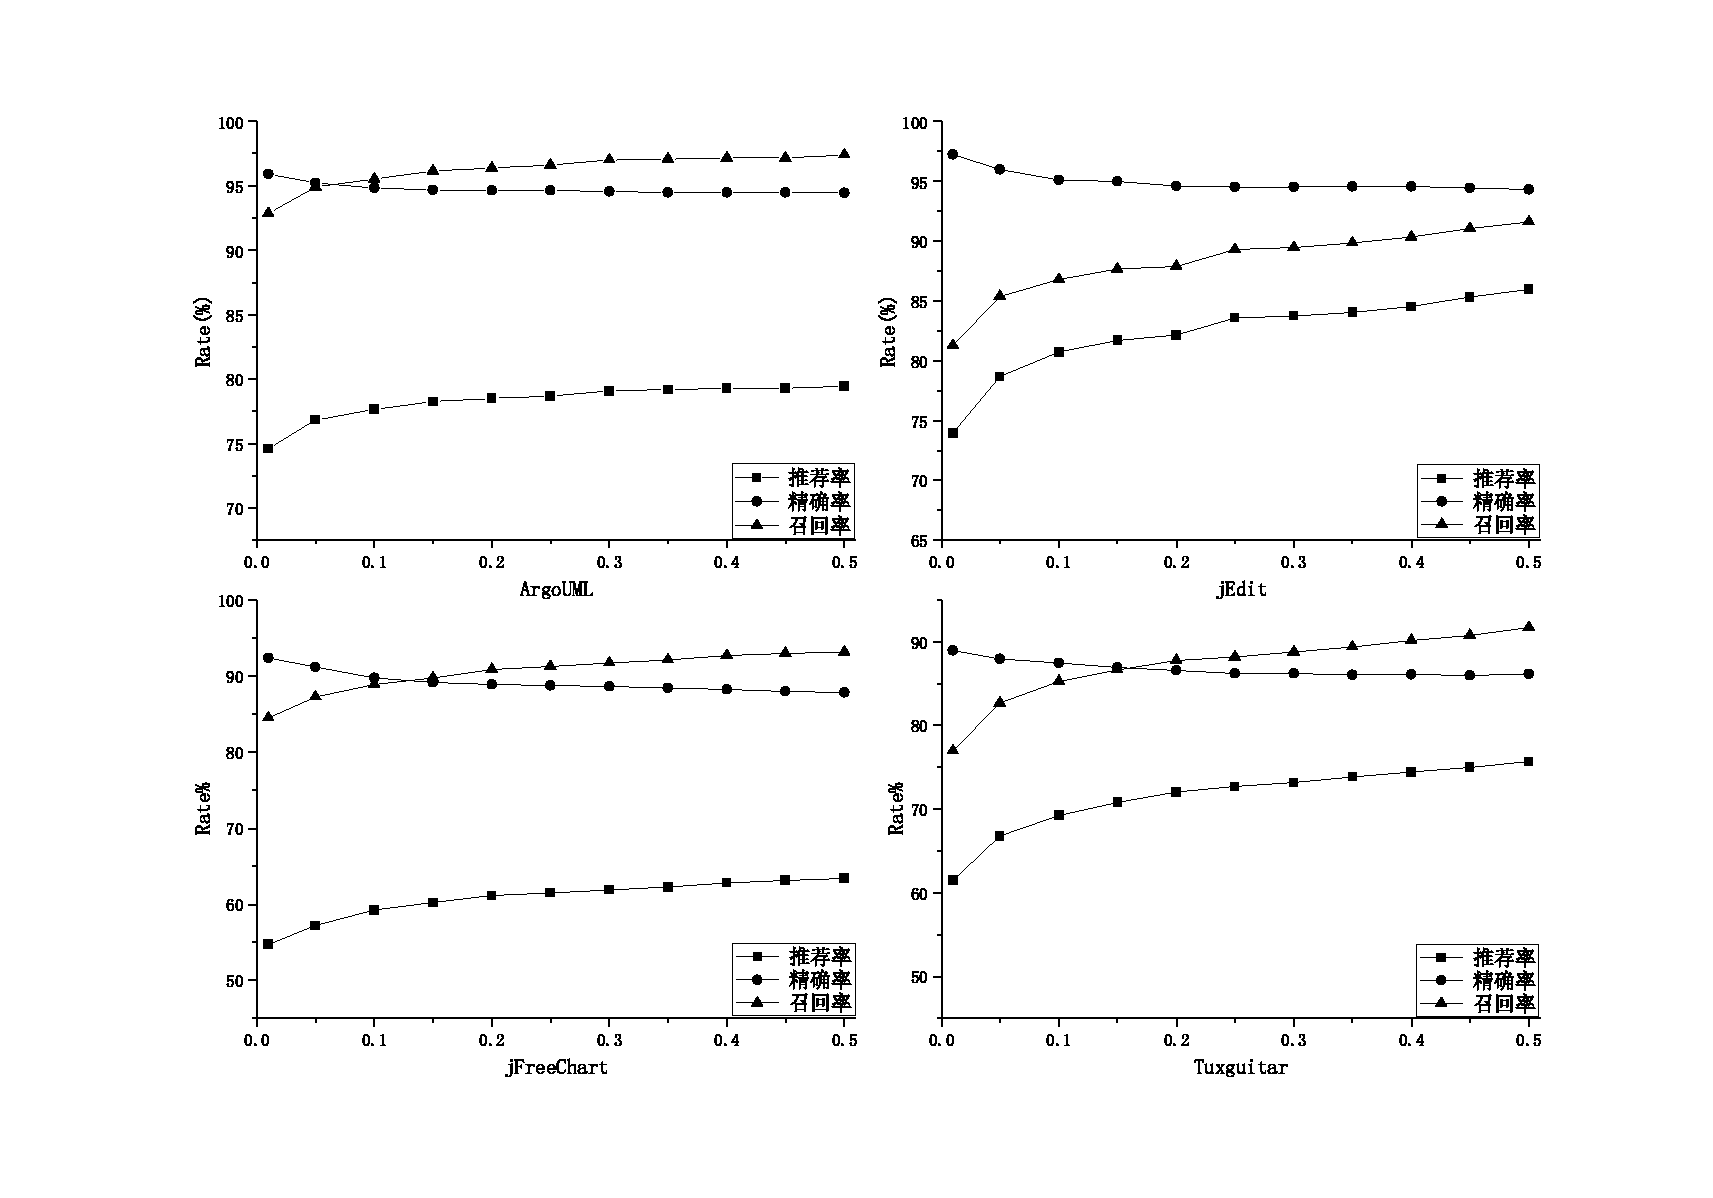
\includegraphics[width = 1.0\textwidth]{bayesgraph/creatingallfree.pdf}
\bicaption[creatingallfree]{}{全属性组维护自由实验效果}
{Fig.$\!$}{The effectiveness for all attributes of clone consistency free}
\vspace{-1em}
\end{figure}

由图~\ref{creatingallfree}~中可以看出,本文方法在预测不需要一致性维护的克隆创建实例时,在四个系统上均取得了较好效果。根据预测结果,四个系统的精确率介于86.2\% - 97.2\%之间,同时召回率也达到较高值,介于77.0\% - 97.4\%之间。其中,ArgoUML系统的预测效果最好,jEdit和jFreeChart系统的预测效果次之,Tuxguitar的预测效果相对最差,但也达到了一个较高的预测效果。
ArgoUML之所以有最好的预测效果是因为其拥有最多的克隆创建实例(2574个)。同时,jEdit与jFreeChart的预测效果相差不大,但是jEdit仅有560个不需要维护的创建实例,jFreeChart有超过2000个实例。因此,预测的效果与训练集规模大小和训练集样本分布(不平衡性)均有关系。在预测克隆代码一致性维护需求时,应该尽量扩大训练集的规模,并且选择向数据较多的一类实例进行预测,从而达到最佳的预测效果。

最后,由图~\ref{creatingallfree}~和表~\ref{copysta}~中可以看出,本文的推荐率达到了一个合理的水平, 和系统中不需要一致性维护的克隆实例比例相差不大。同时,阈值会对预测结果产生一定的影响,其中准确率会随着阈值的升高而缓慢降低,召回率会随着阈值的升高而缓慢增大。但是,阈值所产生的影响不大,四个系统在不同的阈值的准确率和召回率均达到了较高水平。这说明本章的方法以较好的稳定性预测满足一致性维护需求自由的克隆创建实例。
因此,在使用全部属性预测不需要一致性维护的克隆创建实例时,可以达到一个较好地预测效果。


%%%%全属性实验同样使用全部属性在四个实验系统上进行评估,实验结果如表~\ref{copyallfree}~所示。由表中可以看出,本文方法在预测不需要一致性维护的克隆创建实例时,在四个系统上均取得了较好效果。根据预测结果,四个系统的精确率介于86.6--97.22\%之间,同时召回率也达到较高值,介于76.97--96.39\%之间。由表~\ref{copyallfree}~和表~\ref{copysta}~中可以看出,本文的推荐率达到了一个合理的水平, 和系统中不需要一致性维护的克隆实例比例相差不大。同时,阈值对预测结果的影响不大,准确度会随着阈值的降低而缓慢增大。四个系统在不同的阈值的准确度均较高。
%%%%
%%%%因此,本章方法在使用全属性在贝叶斯网络作为分类器时,可以达到一个较好的预测效果。

%%%%%五个阈值的实验表
%%%%%\begin{table}[htbp]
%%%%%\bicaption[copyallfree]{}{全属性组维护自由实验效果}
%%%%%{Table$\!$}{The effectiveness for all attribute of clone consistency free}
%%%%%\vspace{0.5em}
%%%%%\centering
%%%%%\wuhao
%%%%%\begin{tabular}{ccccc}
%%%%%\toprule[1.5pt]
%%%%%{系统}&{阈值}&{推荐率(\%)}&{精确率(\%)}&{召回率(\%)}\\
%%%%%\midrule[1pt]
%%%%%\multirow{5}{*}{ArgoUML}
%%%%%&0.01&	74.61&	95.91&	92.85\\
%%%%%&0.05&	76.83&	95.21&	94.91\\
%%%%%&0.1&	77.63&	94.83&	95.53\\
%%%%%&0.15&  78.26&	94.68&	96.15\\
%%%%%&0.2&	78.47&	94.66&	96.39\\
%%%%%\hline
%%%%%\multirow{5}{*}{jEdit}
%%%%%&0.01&	73.93&	97.22&	81.25\\
%%%%%&0.05&	78.67&	95.98&	85.36	\\
%%%%%&0.1&	80.73&	95.11&	86.79	\\
%%%%%&0.15&	81.67&	94.97&	87.68	\\
%%%%%&0.2&	82.15&	94.62&	87.86	\\
%%%%%\hline
%%%%%\multirow{5}{*}{jFreeChart}
%%%%%&0.01&	54.69&	92.40&	84.50\\
%%%%%&0.05&	57.22&	91.23&	87.28\\
%%%%%&0.1&	59.24&	89.72&	88.87\\
%%%%%&0.15&	60.22&	89.15&	89.77\\
%%%%%&0.2&	61.14&	88.87&	90.86\\
%%%%%\hline
%%%%%\multirow{5}{*}{Tuxguitar}
%%%%%&0.01&	61.51&	88.96&	76.97\\
%%%%%&0.05&	66.83&	87.96&	82.68\\
%%%%%&0.1&	69.28&	87.47&	85.24\\
%%%%%&0.15&	70.82&	86.96&	86.61\\
%%%%%&0.2&	72.08&	86.60&	87.80\\
%%%%%\bottomrule[1.5pt]
%%%%%\end{tabular}
%%%%%\end{table}

(2)属性组实验

针对不同的属性组进行了属性组实验,实验结果如图~\ref{creatingsetfree}~所示。其中,使用“RR”表示推荐率,“P”表示精确率,“R”表示召回率。并同时使用不同的后缀表示不同属性组的实验结果,其中“All”为全属性组实验结果,“Code”表示仅使用代码属性的实验结果,“Context”表示上下文属性的实验结果。

\begin{figure}[h]
\centering
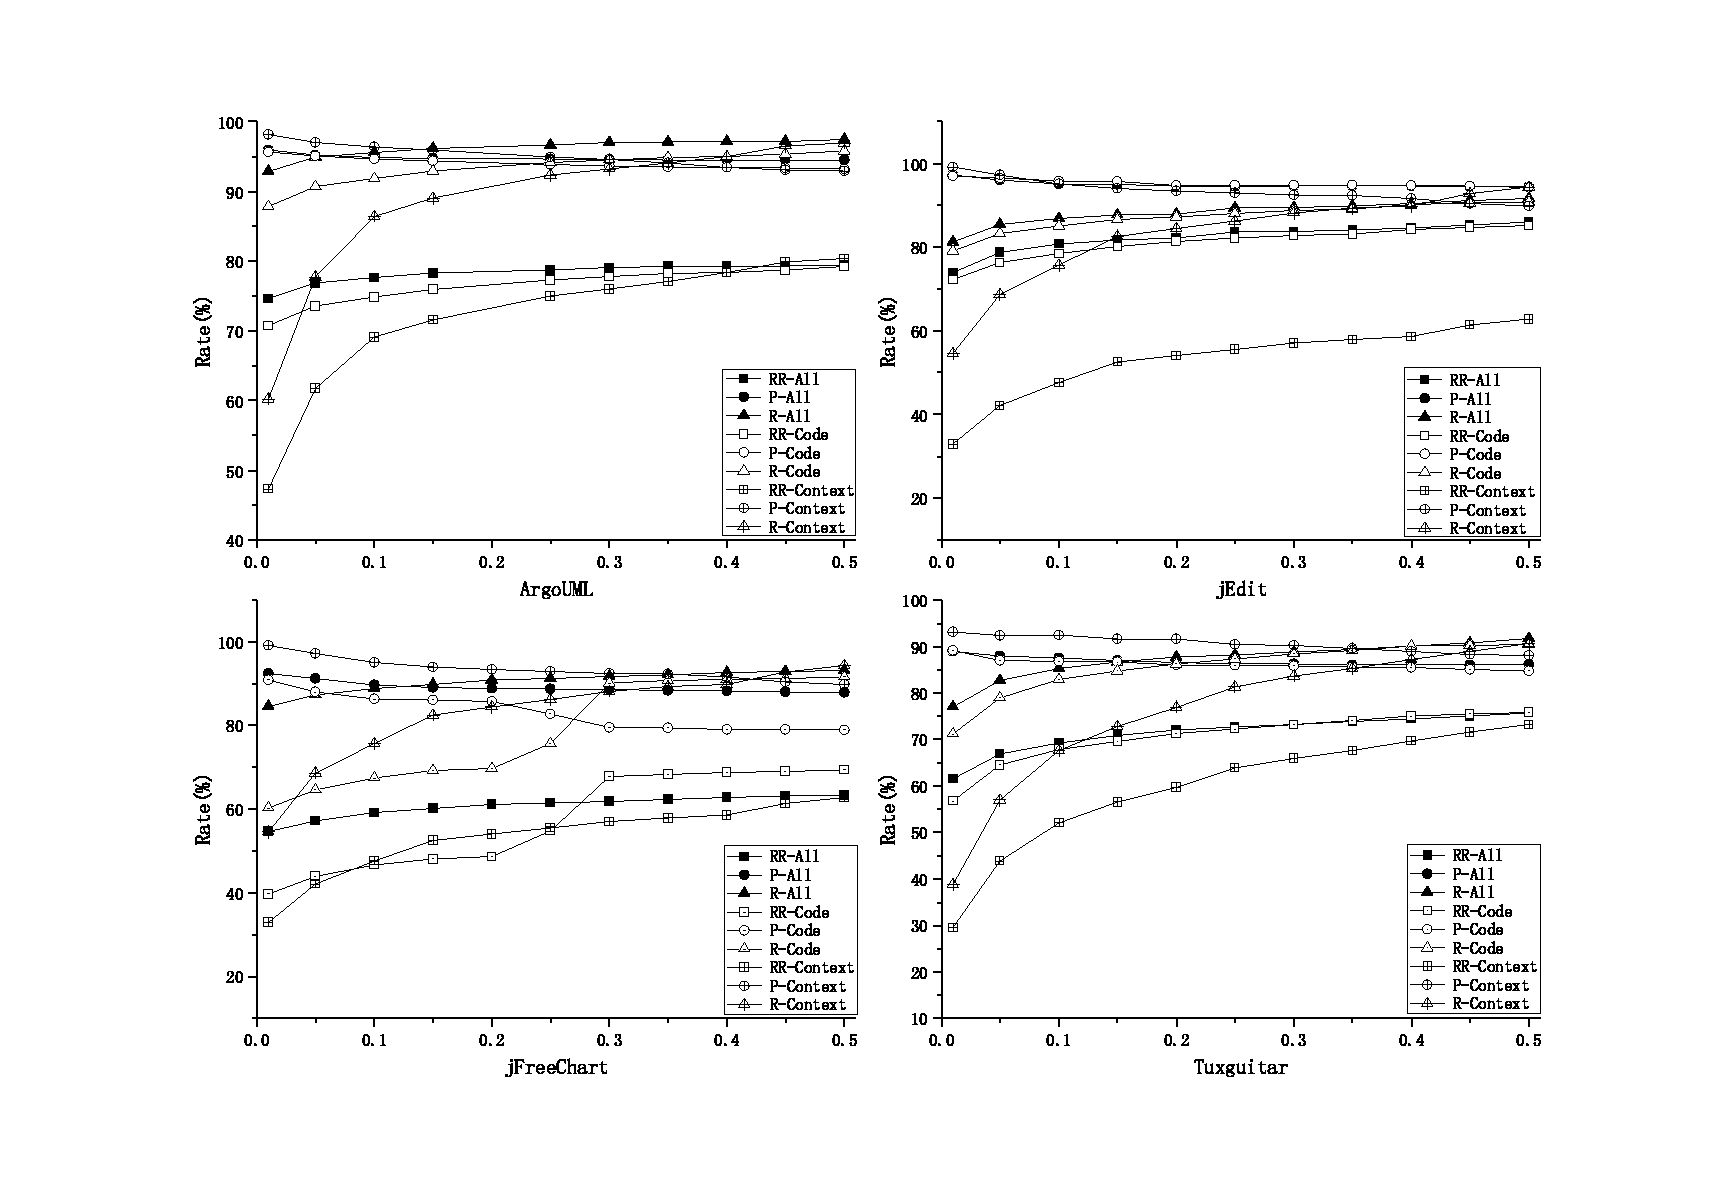
\includegraphics[width = 1.0\textwidth]{bayesgraph/creatingsetfree.pdf}
\bicaption[creatingsetfree]{}{属性组维护自由实验效果}
{Fig.$\!$}{The effectiveness for attribute set of clone consistency free}
\vspace{-1em}
\end{figure}

由图~\ref{creatingsetfree}~中可以看出,代码属性实验的预测效果依然较好,但和全属性实验对比发现代码属性实验的召回率下降,精确率除jEdit中少数几个之外也全部下降,因此本章提取的代码属性对预测作用具有积极意义。在上下文属性实验中,预测结果除jEdit系统外精确率提高,但是系统的召回率却大大降低。因此,下上下文属性对系统的精确率影响较大,而代码属性对系统的召回率影响较大,同时两者对于预测都起到了积极的作用。

因此,本章建议在进行预测时,保留所有的属性进行预测。因为某些属性可能对其它尚未验证的系统具有积极的作用。

%%%%实验结果如表~\ref{copysetfree}~所示,其中左侧为代码属性,右侧为上下文属性。由表~\ref{copysetfree}~和表~\ref{copyallfree}~中可以看出,代码属性实验的预测效果依然较好,但和全属性实验对比发现代码属性实验的召回率下降,精确率除jEdit中少数几个之外也全部下降,因此本文提取的代码属性对预测作用具有积极意义。在上下文属性实验中,预测结果除jEdit系统外精确率提高,但是系统的召回率却大大降低。因此,下上下文属性对系统的精确率影响较大,而代码属性对系统的召回率影响较大,同时两者对于预测都起到了积极的作用。
%%%%
%%%%因此,本章建议在进行预测时,保留所有的属性进行预测。因为某些属性可能对其它尚未验证的系统具有积极的意义。
%%%%
%%%%\begin{table}[htbp]
%%%%\bicaption[copysetfree]{}{属性组维护自由实验效果}
%%%%{Table$\!$}{The effectiveness for attribute set of clone consistency free}
%%%%\vspace{0.5em}
%%%%\centering
%%%%\wuhao
%%%%\begin{tabular}{cccccccc}
%%%%\toprule[1.5pt]
%%%%\multirow{2}{*}{实验系统}&\multirow{2}{*}{阈值}&\multicolumn{3}{c}{代码属性(\%)}&\multicolumn{3}{c}{上下文属性(\%)}\\
%%%%\cline{3-8}
%%%%&&推荐率&精确率&召回率&推荐率&精确率&召回率\\
%%%%\midrule[1pt]
%%%%\multirow{5}{*}{ArgoUML}
%%%%&0.01&	70.75&	95.64&	87.80&	47.31&	98.10&	60.22\\
%%%%&0.05&	73.53&	95.07&	90.71&	61.74&	96.99&	77.70\\
%%%%&0.1&	74.82&	94.60&	91.84&	69.22&	96.24&	86.44\\
%%%%&0.15&	75.93&	94.32&	92.93&	71.53&	95.90&	89.01\\
%%%%&0.2&	76.59&	94.02&	93.43&	73.59&	95.52&	91.22\\
%%%%\hline
%%%%\multirow{5}{*}{jEdit}
%%%%&0.01&	72.20&    96.94&	79.11&	32.95&	99.10&	54.60\\
%%%%&0.05&	76.30&	96.48&	83.21&	42.19&	97.25&	68.60\\
%%%%&0.1&	78.67&	95.78&	85.18&	47.74&	95.02&	75.86\\
%%%%&0.15&	80.09&	95.66&	86.61&	52.55&	93.95&	82.56\\
%%%%&0.2&	81.36&	94.76&	87.14&	54.10&	93.36&	84.45\\
%%%%\hline
%%%%\multirow{5}{*}{jFreeChart}
%%%%&0.01&	39.69&	90.94&	60.36&	32.95&	99.10&	54.60\\
%%%%&0.05&	43.94&	87.96&	64.63&	42.19&	97.25&	68.60\\
%%%%&0.1&	46.70&	86.32&	67.41&	47.74&	95.02&	75.86\\
%%%%&0.15&	48.07&	86.16&	69.25&	52.55&	93.95&	82.56\\
%%%%&0.2&	48.66&	85.71&	69.75&	54.10&	93.36&	84.45\\
%%%%\hline
%%%%\multirow{5}{*}{Tuxguitar}
%%%%&0.01&	56.75&	89.15&	71.16&	29.60&	93.14&	38.78\\
%%%%&0.05&	64.52&	86.98&	78.94&	43.88&	92.34&	56.99\\
%%%%&0.1&	67.88&	86.80&	82.87&	51.99&	92.46&	67.62\\
%%%%&0.15&	69.56&	86.62&	84.74&	56.54&	91.58&	72.83\\
%%%%&0.2&	71.24&	86.05&	86.22&	59.69&	91.56&	76.87\\
%%%%\bottomrule[1.5pt]
%%%%\end{tabular}
%%%%\end{table}

\BiSubsubsection{一致性维护实验}
{The Experiment for Meeting Clone Creating Consistency}

本节对需要一致性维护的克隆创建实例进行预测评估。将关注需要一致性维护的克隆创建实例,由于其在演化过程中可能会引发一致性变化,因此需要警告程序开发人员谨慎的执行复制和粘贴操作,避免额外的维护代价。实验同样使用三个度量对方法进行评估:警告率、精确率和召回率。其中,警告率(Warning Rate,WR)指所警告的需要一致性维护的克隆创建实例,即预测为需要一致性维护的实例与系统中全部实例的比值。

%%%\begin{itemize}
%%%\item	
%%%警告率(Warning Rate):
%%%指所警告的需要一致性维护的克隆创建实例,即预测为需要一致性维护的实例与系统中全部实例的比值。这些克隆实例可能会引发一致性变化和额外维护代价。
%%%\item	
%%%精确率(Precision):
%%%指警告为需要一致性维护的克隆创建实例的精确率,即在所预测的需要一致性维护的实例中,正确预测的实例与全部警告实例的比值。
%%%\item	
%%%召回率(Recall):指所警告的需要一致性维护的克隆创建实例的召回率,即预测为需要一致性维护的实例与系统中的需要一致性维护实例的比值。
%%%\end{itemize}

(1)全属性实验结果

全属性实验使用全部属性在四个实验系统上进行评估,实验结果如图~\ref{creatingallmeeting}所示。图中的横坐标表示阈值,设置阈值从0.50到1.0,图中的纵坐标为评价指标的数值。

\begin{figure}[h]
\centering
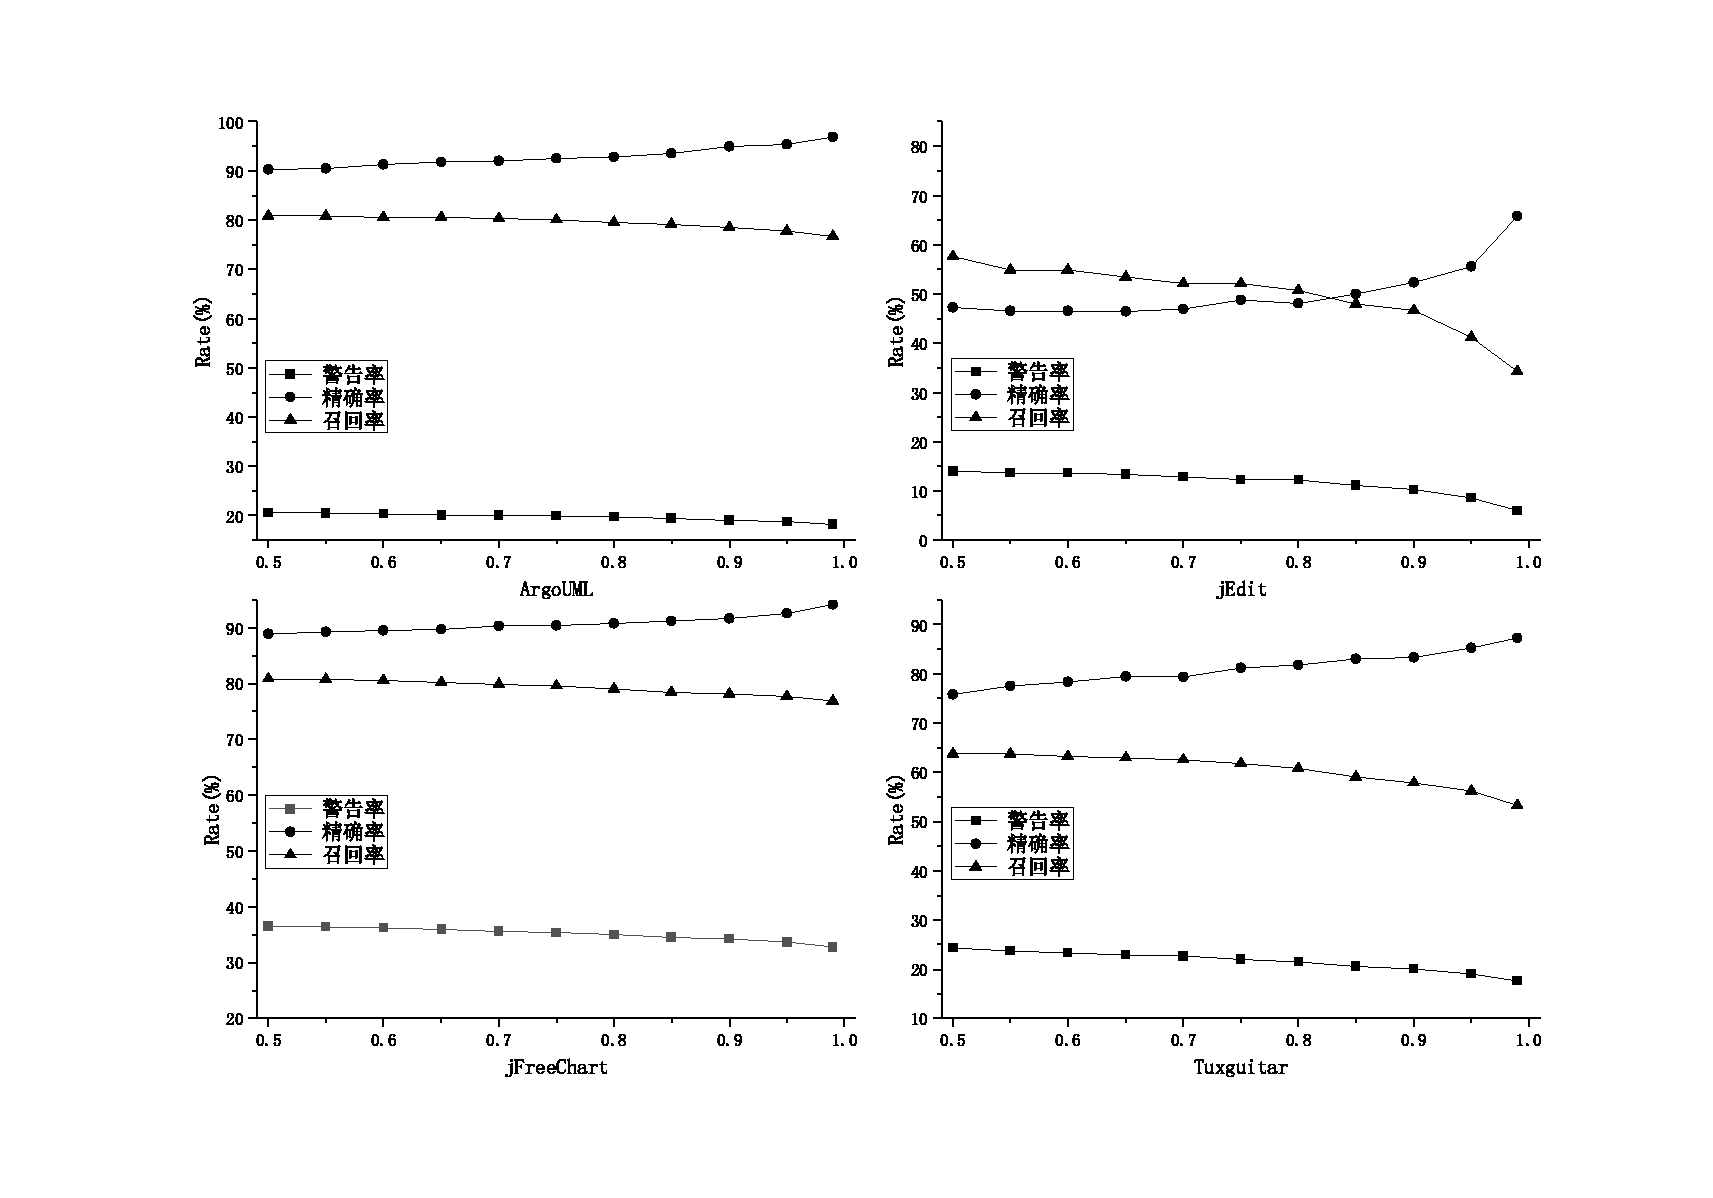
\includegraphics[width = 1.0\textwidth]{bayesgraph/creatingallmeeting.pdf}
\bicaption[creatingallmeeting]{}{全属性组需要维护的全属性实验效果}
{Fig.$\!$}{The effectiveness for all attributes of clone consistency}
\vspace{-1em}
\end{figure}

由图中可以看出,本章方法在预测需要一致性维护的克隆创建实例时,也取得了较好的预测效果。首先,系统ArgoUML和jFreeChart在不同阈值下取得了不错的预测效果:精确率介于75.8\% - 96.9\%之间,召回率介于76.6\% - 80.9\%之间。系统ArgoUML和jFreeChart的训练集最大,分别拥有766和1353个需要维护的克隆代码创建实例。因此,可以较好的训练机器学习模型,并取得四个系统中最好的预测效果。然后,尽管Tuxguitar的预测效果没有另外两个系统的预测结果好,但是其精确率在75.8\% - 87.3\%,召回率为53.3\% - 63.7\%。最后,jEdit系统的预测效果不够理想,其准确度和召回率仅在50\%左右。分析其原因可能为jEdit中训练数据过少导致模型不完全,数据集仅有73个复制粘贴实例。尽管如此,jEdit的预测结果的准确度依然高于其系统自身的一致性维护需求的比例(11.53\%),在jEdit系统上的预测依然是有效的。因此,在预测克隆代码一致性时,扩大训练集的规模对于提高预测效果具有积极的意义。

对于四个实验系统,本章所构建的模型均具有有十分合理的警告率,警告率十分接近于满足一致性维护需求的克隆变化实例的比例(如表~\ref {copysta}~中所示)。虽然阈值的变化可以影响预测的精确率和召回率,但影响并不是十分的剧烈,其中除jEdit对精确率的影响要大于对召回率的影响。尽管如此,在不同的阈值下,本章构建模型的精确率依然达到了较高的水平。因此开发人员可以非常自信地依赖于本章模型的预测结果。然而,本章方法的召回率没有达到准确率的效果,但仍需进一步增强预测模型的召回能力,需要进一步的深入研究。

因此,在使用全部属性预测需要一致性维护的克隆创建实例时,可以达到一个较好地预测效果。但是, 对于部分缺少训练数据的系统(如jEdit系统),本文建议预测不需要一致性维护的克隆创建实例,从而确保达到最佳的预测效果。

%%%%全属性实验同样使用全部属性在四个实验系统上进行评估,实验结果如表~\ref{copyallmeeting}所示。由表中可以看出,除jEdit外其余系统在不同阈值下取得了可以不错的效果:精确率介于75.79\%-94.94\%之间,召回率介于57.87\%-80.86\%之间。jEdit的预测效果不够理想,其准确度和召回率仅在50\%左右。分析其原因可能为jEdit中训练数据过少导致模型不完全,数据集仅有73复制粘贴实例,仍需要进一步的研究确定。尽管如此,jEdit的预测结果的准确度依然高于其系统自身的一致性维护需求的比例(11.53\%)。因此,在jEdit系统上依然提高了预测的精度,也是有效的。最后,对于四个实验系统,本文所构建的模型均具有有十分合理的警告率,警告率十分接近于满足一致性维护需求的克隆变化实例的比例(如表~\ref {copysta}~中所示)。
%%%%
%%%%虽然阈值的变化可以影响预测的精确率和召回率,但影响并不是十分的剧烈,其中除jEdit对精确率的影响要大于对召回率的影响。尽管如此,在不同的阈值下,本文构建模型的精确率依然达到了较高的水平。因此开发人员可以非常自信地依赖于本文模型的预测结果。然而,本文方法的召回率没有达到准确两率的效果,但仍需进一步增强预测模型的召回能力,这需要进一步的深入研究。
%%%%
%%%%\begin{table}[htbp]
%%%%\bicaption[copyallmeeting]{}{需要维护的全属性实验效果}
%%%%{Table$\!$}{The effectiveness for all attributes of clone consistency}
%%%%\vspace{0.5em}
%%%%\centering
%%%%\wuhao
%%%%\begin{tabular}{ccccc}
%%%%\toprule[1.5pt]
%%%%{实验系统}&{阈值}&{警告率(\%)}&{精确率(\%)}&{召回率(\%)}\\
%%%%\midrule[1pt]
%%%%\multirow{5}{*}{ArgoUML}
%%%%&0.9&	18.95&	94.94&	78.46\\
%%%%&0.8&	19.64&	92.84&	79.50\\
%%%%&0.7&	20.03&	91.93&	80.29\\
%%%%&0.6&	20.24&	91.27&	80.55\\
%%%%&0.5&	20.54&	90.23&	80.81\\
%%%%\hline
%%%%\multirow{5}{*}{jEdit}
%%%%&0.9&	10.27&	52.31&	46.58\\
%%%%&0.8&	12.16&	48.05&	50.68\\
%%%%&0.7&	12.80&	46.91&	52.05\\
%%%%&0.6&	13.59&	46.51&	54.79\\
%%%%&0.5&	14.06&	47.19&	57.53\\
%%%%\hline
%%%%\multirow{5}{*}{jFreeChart}
%%%%&0.9&	34.25&	91.67&	78.12\\
%%%%&0.8&	35.03&	90.75&	79.08\\
%%%%&0.7&	35.56&	90.31&	79.90\\
%%%%&0.6&	36.19&	89.49&	80.56\\
%%%%&0.5&	36.57&	88.87&	80.86\\
%%%%\hline
%%%%\multirow{5}{*}{Tuxguitar}
%%%%&0.9&	20.08&	83.28&	57.87\\
%%%%&0.8&	21.48&	81.76&	60.77\\
%%%%&0.7&	22.74&	79.38&	62.47\\
%%%%&0.6&	23.30&	78.38&	63.20\\
%%%%&0.5&	24.28&	75.79&	63.68\\
%%%%\bottomrule[1.5pt]
%%%%\end{tabular}
%%%%\end{table}

(2)属性组实验结果

类似的,对于一致性维护需求实例,表~\ref{creatingsetmeeting}~给出了属性组实验结果。图中使用“WR”表示警告率,“P”表示精确率,“R”表示召回率。并同时使用不同的后缀表示不同属性组的实验结果,其中“All”为全属性组实验结果,“Code”表示仅使用代码属性的实验结果,“Context”表示上下文属性的实验结果。

\begin{figure}[h]
\centering
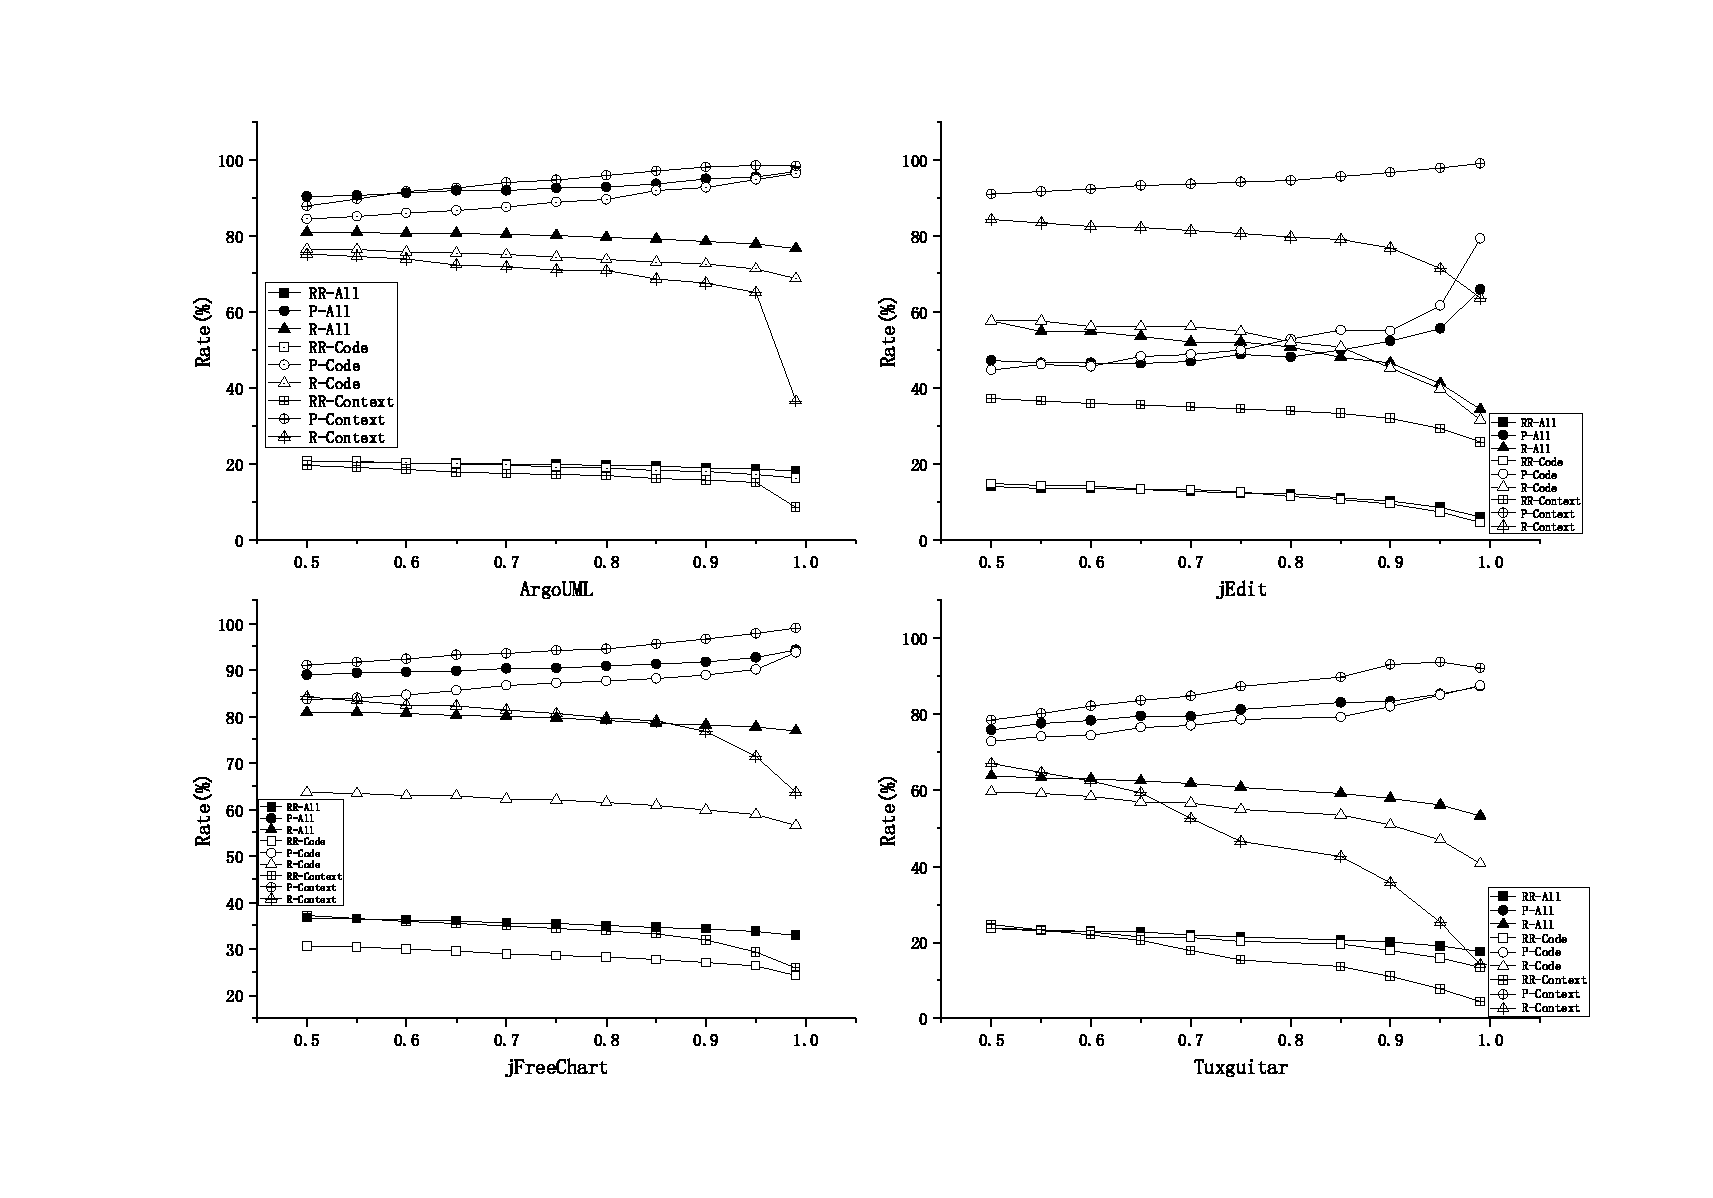
\includegraphics[width = 1.0\textwidth]{bayesgraph/creatingsetmeeting.pdf}
\bicaption[creatingsetmeeting]{}{需要维护的属性组实验效果}
{Fig.$\!$}{The effectiveness for attribute set of clone consistency}
\vspace{-1em}
\end{figure}



由图中可以看出,代码属性的实验结果明显不如全属性组实验,但仍在可接受的范围之内,说明代码属性对预测有积极的影响。上下文属性实验中,当仅仅使用上下文属性时部分系统的实验效果要优于全属性组实验,而部分系统的结果不如全属性组实验。因此,上下文属性对不同的系统所起到的作用并非一样的。上下文属性和代码属性都具有积极地意义,而上下文属性的影响更大。


%%%%%类似的,对于一致性维护需求实例,表~\ref{copysetmeeting}~给出了属性组实验结果。由表中可以看出,代码属性的实验结果明显不如全属性组实验,但仍在可接受的范围之内,说明代码属性对预测有积极的影响。上下文属性实验中,当仅仅使用上下文属性时部分系统的实验效果要优于全属性组实验,而部分系统的结果不如全属性组实验。因此,上下文属性对不同的系统所起到的作用并非一样的。上下文属性和代码属性都具有积极地意义,而上下文属性的影响更大。
%%%%%
%%%%%\begin{table}[htbp]
%%%%%\bicaption[copysetmeeting]{}{需要维护的属性组实验效果}
%%%%%{Table$\!$}{The effectiveness for attribute set of clone consistency}
%%%%%\vspace{0.5em}\centering\wuhao
%%%%%\begin{tabular}{cccccccc}
%%%%%\toprule[1.5pt]
%%%%%\multirow{2}{*}{系统}&\multirow{2}{*}{阈值}&\multicolumn{3}{c}{ 代码属性(\%)}&\multicolumn{3}{c}{上下文属性(\%)}\\
%%%%%\cline{3-8}
%%%%%&&{警告率}&{精确率}&{召回率}&{警告率}&{精确率}&{召回率}\\
%%%%%\midrule[1pt]
%%%%%\multirow{5}{*}{ArgoUML}
%%%%%&0.9&	17.96&	92.67&	72.58&	15.78&	98.10&	67.49\\
%%%%%&0.8&	18.89&	89.54&	73.76&	16.98&	95.77&	70.89\\
%%%%%&0.7&	19.67&	87.52&	75.07&	17.51&	94.02&	71.80\\
%%%%%&0.6&	20.21&	85.93&	75.72&	18.50&	91.59&	73.89\\
%%%%%&0.5&	20.78&	84.44&	76.50&	19.64&	87.80&	75.20\\
%%%%%\hline
%%%%%\multirow{5}{*}{jEdit}
%%%%%&0.9&	9.48&	55.00&	45.21&	31.91&	96.65&	76.72\\
%%%%%&0.8&	11.37&	52.78&	52.05&	33.87&	94.47&	79.60\\
%%%%%&0.7&	13.27&	48.81&	56.16&	34.94&	93.54&	81.30\\
%%%%%&0.6&	14.22&	45.56&	56.16&	35.89&	92.30&	82.41\\
%%%%%&0.5&	14.85&	44.68&	57.53&	37.20&	90.97&	84.18\\
%%%%%\hline
%%%%%\multirow{5}{*}{jFreeChart}
%%%%%&0.9&	27.04&	88.90&	59.79&	31.91&	96.65&	76.72\\
%%%%%&0.8&	28.19&	87.57&	61.42&	33.87&	94.47&	79.60\\
%%%%%&0.7&	28.85&	86.61&	62.16&	34.94&	93.54&	81.30\\
%%%%%&0.6&	29.92&	84.61&	62.97&	35.89&	92.30&	82.41\\
%%%%%&0.5&	30.57&	83.58&	63.56&	37.20&	90.97&	84.18\\
%%%%%\hline
%%%%%\multirow{5}{*}{Tuxguitar}
%%%%%&0.9&	17.91&	82.03&	50.85&	11.06&	93.04&	35.59\\
%%%%%&0.8&	20.22&	78.55&	54.96&	15.40&	87.27&	46.49\\
%%%%%&0.7&	21.48&	76.55&	56.90&	20.50&	83.62&	59.32\\
%%%%%&0.6&	23.02&	74.16&	59.08&	23.30&	80.18&	64.65\\
%%%%%&0.5&	24.14&	71.88&	60.05&	26.94&	74.81&	69.73\\
%%%%%\bottomrule[1.5pt]
%%%%%\end{tabular}
%%%%%\end{table}

\BiSubsection{与其它方法的对比}
{Comparing with Wang’s Method}

Wang等人也使用贝叶斯网络对克隆代码创建时的一致性维护需求进行了预测研究\cite{wang2014predicting}。Wang等人在四个实验系统上进行了实验,其中两个实验系统是微软内部的系统(无法获取实验系统信息 ),另外两个系统为开源系统jFreeChart和Tuxguitar。因此,针对系统jFreeChart和Tuxguitar,本节将本章的实验结果与Wang的方法进行对比,验证本章所提出方法的有效性。方法对比的实验结果如表~\ref{comparecopysta}~和表~\ref{comparecopyprediction}~所示。

表~\ref{comparecopysta}~是所收集到的克隆创建实例信息对比。由表中可以看出,本章所收集的克隆创建实例数量要多于Wang所收集的实例数量。

\begin{table}[htbp]
\bicaption[comparecopysta]{}{实验系统的克隆创建实例信息统计对比}
{Table$\!$}{The comparing statistics for clone creating instances in two projects}
\vspace{0.5em}
\centering
\wuhao
\begin{tabular}{cccc}
\toprule[1.5pt]
~\multirow{2}{*}{实验系统}& \multicolumn{2}{c}{克隆变化实例的数量(比例)} & \multirow{2}{*}{总数}\\ 
 \cline{2-3}
~&{不需要维护} &{需要维护} & ~\\
\midrule[1pt]
jFreeChart(本章)&	2013(59.8\%)&	1353(40.2\%)&	3366\\
jFreeChart(Wang)&1059(92.2\%)&	89(7.8\%)&	1148\\
Tuxguitar(本章)&	1016(71.1\%)&	413(28.9\%)&	1429\\
Tuxguitar(Wang)&384(86.5\%)&	60(13.5\%)&	444\\
\bottomrule[1.5pt]
\end{tabular}
\end{table}

表~\ref{comparecopyprediction}~是本章方法与Wang的方法的预测效果对比。表中使用平均精确度(Average Precision)和平均召回率(Average Recall)评估预测效果,即加权平均需要和不需要一致性维护的预测结果。由表中可以看出,本章所提出的方法具有更好的预测能力。具体地,对于jFreeChart系统,本章方法的平均精确率为88.3\%,平均召回率为88.2\%,然而Wang的方法仅为58.3\%和63.0\%。对于Tuxguitar系统,本章方法的平均精确率为83.1\%,平均召回率为83.6\%,然而Wang的方法仅为61.5\%和60.1\%。

\begin{table}[htbp]
\bicaption[comparecopyprediction]{}{克隆创建实例的预测效果对比}
{Table$\!$}{The comparing effectiveness for clone creating instances in two projects}
\vspace{0.5em}
\centering
\wuhao
\begin{tabular}{ccc}
\toprule[1.5pt]
{实验系统}&{平均精确率(\%)} &{平均召回率(\%)}\\ 
\midrule[1pt]
jFreeChart(本章)&	88.3& 88.2\\
jFreeChart(Wang)&58.3&	63.0\\
Tuxguitar(本章)&	83.1&	83.6\\
Tuxguitar(Wang)&61.5&	60.1\\
\bottomrule[1.5pt]
\end{tabular}
\end{table}

本章方法之所以优于Wang方法主要有两个原因。第一个原因是本章方法改进了表示克隆创建实例的属性特征。首先,摒弃了与克隆创建实例中复制和粘贴操作关联较小的历史属性。然后,扩展了表示克隆创建实例的代码属性和上下文属性,提取了更多的属性描述克隆创建实例。第二个原因是本章方法所收集到的克隆创建实例要多于Wang的方法。本文使用经典的克隆检测工具NiCad检测系统存在的克隆代码,并用于收集克隆创建实例。在使用克隆创建实例进行训练机器学习模型时,本章使用更多的克隆创建实例使得所训练的机器学习模型更为完善,具有更好的预测效果。

\BiSubsection{讨论}
{Discussion}

本节从不同的角度评估了本章所提出的克隆代码创建的一致性维护需求预测,同时对不需要和需要一致性维护需求的克隆创建实例进行了预测,并从不同的角度评估了不同的机器学习方法的预测能力。

在有效性验证实验中,五种机器学习方法都可应用于克隆代码的一致性维护需求预测中,并具有相似的预测能力,预测结果具有较高的精确率、召回率和F值。更重要的是,不同机器学习模型的预测能力仅具有较小的差异,但支持向量机方法拥有相对最佳的预测效果。因此,建议优先推荐使用支持向量机方法预测克隆代码创建的一致性维护需求。与此同时,所提取的属性组作为一个整体在不同机器学习方法的预测中,同样起到了积极的作用。因此,建议软件开发人员在预测时保留所有的属性组进行创建时一致性预测。

在使用模式实验中,全属性实验结果表明:本章所构建的模型在一致性维护需求和一致性维护自由的实验上,均具有高效地预测能力。同时,本文所提取的代码属性和上下文属性对克隆创建实例的一致性维护需求的预测起到了积极的作用。但在不同系统中,所产生的影响程度不一致。因此,建议维护人员使用全属性组进行克隆创建实例的一致性维护需求预测,从而将其使用到其它未验证的系统中,使之达到最佳的预测效果。
%最后,数据的规模与样本分布情况。。。。
\BiSection{本章小结}
{Summary of this Chapter}

通过复制和粘贴操作复用既有代码可以向系统中引入新创建的克隆代码,然而在其演化过程中可能会发生一致性变化,从而导致额外的维护代价。为帮助软件开发人员从规避克隆代码产生的角度降低克隆代码的额外维护代价,本章提出了克隆代码创建一致性维护需求预测方法。可在克隆代码创建时(复制和粘贴时),预测新创建的克隆代码的一致性维护需求,根据预测结果决定是否执行该复制粘贴操作。构建了软件系统的克隆家系,并通过识别克隆家系的根节点收集克隆创建实例(复制和粘贴操作)。使用不同的属性组表示克隆创建实例,使用代码属性表示被复制克隆代码,使用上下文属性表示被粘贴的克隆代码。在四个开源软件系统上进行实验,验证所构建模型的预测能力。实验结果表明本章方法可以以较高的精确率和召回率高效地预测克隆代码的一致性维护需求。此外,所提取的两组属性组在预测中均起到了积极的作用,但是对精确率和召回率有不同的影响。

%本文的主要贡献如下:
%(1)本文定义了新的克隆代码一致性变,并根据其定义了克隆代码的一致性维护需求,可以更为准确的标识克隆代码的一致性维护代价;
%(2)本文使用并扩展代码属性和上下文属性两组属性组,实验结果表明所使用的属性在克隆一致性维护需求的预测中起到了积极的作用;
%(3)本文预测克隆代码的一致性维护需求,不仅在贝叶斯网络分类器上进行了实验评估,还在一般分类器上进行了实验验证,实验结果表明本文方法具有一般性,可以适用于一般的机器学习方法。
% !Mode:: "TeX:UTF-8" 

\BiChapter{基于贝叶斯网络的克隆变化时一致性维护预测方法}
{Predicting Clone Consistency-Requirement Based on Bayesian Network at Clone Changing Time}

\BiSection{引言}
{Introduction}

由于日益增长的软件开发的需求,开发人员在软件开发过程中经常复用既有代码,从而向系统中引入了大量的克隆代码。克隆代码会随着软件系统演化,在其演化过程中,克隆组内的某一克隆代码片段可能会被软件开发员修改而发生变化。由于克隆组内的克隆片段彼此相似,克隆片段变化可能会导致其所在克隆组未来演化过程中的一致性变化。遗忘这种克隆代码的一致性变化,会引入与之相关的克隆一致性缺陷,从而增大系统的维护代价。本文将由克隆代码变化所导致的其所在克隆组未来演化过程中发生的一致性变化,称为克隆代码变化时的一致性维护需求。在克隆代码变化时时预测克隆代码的一致性维护需求,可以帮助避免克隆代码的一致性缺陷,从而帮助提高软件质量和可维护性。

鉴于此,本章与第三章相似,在定义克隆代码变化时的一致性变化和一致性维护需求的基础上,使用机器学习中的贝叶斯网络方法在克隆代码变化时预测其一致性维护需求。为训练克隆代码变化时一致性预测模型,首先通过构建软件系统的克隆家系来收集系统中所有的克隆变化实例(发生变化的克隆代码)。然后,提取了代码属性、上下文属性和演化属性三组属性值表示克隆代码变化实例。最后,使用贝叶斯网络方法训练机器学习模型,并预测克隆代码变化时的一致性维护需求。在四个开源软件系统上对本章方法进行了评估,实验结果表明本章方法以合理的准确率和召回率有效地预测克隆代码变化时的一致性维护需求。本章所提出的预测方法同样可以帮助开发人员在克隆代码变化时预测克隆代码的一致性,避免克隆变化导致的一致性缺陷,从而提高软件质量和可维护性。

\BiSection{克隆代码变化时一致性维护需求}
{Clone Changing Consistency-Requirement}

\BiSubsection{一致性变化例子}
{An Example of Clone Consistent Change }

在软件开发过程中,复用既有代码是一种常见的软件开发手段,但是也会向软件系统中引入大量的克隆代码。有研究表明软件中的克隆代码可以占到系统代码规模的7\%-23\%\cite{koschke2007survey}。软件中存在的克隆代码不是静止不变的,会随着软件系统进行演化,其演化过程可使用克隆家系进行描述\cite{kim2005empirical}(克隆演化见本文~\ref{ref-evolution}~节)。本文第二章通过分析克隆演化特征发现,在克隆演化过程中,克隆代码的一致性变化往往多于不一致性变化,因此开发人员需要警惕发生变化的克隆代码,并且当发生变化时需要考虑克隆代码的一致性问题。(具体可参考本文~\ref{ref-characteristics}~节)

演化中的克隆变化使得克隆代码变得越来越难以维护,而克隆代码的一致性问题会导致额外的维护代价。当克隆代码发生变化时,程序开发人员需要验证克隆代码的一致性,从而导致维护代价的增加;如果开发人员忘记验证克隆代码的一致性,则可能会向系统中引入新的克隆一致性缺陷在\cite{bettenburg2009empirical} \cite {juergens2009code}。本文第三章研究了克隆代码创建时的一致性维护需求问题,在克隆代码产生时预测克隆代码一致性。在一定程度上可以降低软件的维护代价。但是,值得注意的是,并不是所有的克隆代码都可以被避免。同时,上述方法也无法处理系统中已经存在的克隆代码的一致性变化问题。因此,本章将讨论克隆代码变化时其一致性维护需求问题。

在详细论述本章方法之前,本文先给出一个克隆代码的一致性变化的具体例子,如图~\ref{co-change}~所示。该一致性变化例子来自于软件系统{jEdit}中。在图~\ref{cg1}中给出了$ 3.1.0 $版本中的两个克隆代码片段,它们之间是彼此相似的,可称之为克隆代码。在随着系统演化至$ 3.2.0 $版本时,上述两个克隆代码发生了一致性变化。具体地,$ 3.1.0 $版本中的第9-12行和第15行代码在下一版本$ 3.2.0 $中被开发人员修改。第9-12行,开发人员将{\tt selectionEnd}更改为$ 0 $,并删除了一对花括号。在第15行,开发人员删除了声明语句。如图~\ref{cg2}~所示,这两个被修改的代码片段仍然是彼此相似的克隆代码(仍存在于版本$ 3.2.0 $中的同一克隆组中)。假设程序人员没有对上述两个克隆代码进行一致性维护,这必然会导致克隆代码的一致性缺陷,从而降低软件质量。

\begin{figure}[htbp]
\centering
\subfigure{\label{cg1}}
\addtocounter{subfigure}{-2}
\subfigure[Two clone fragments in one clone group in version $3.1.0$]
{\subfigure[版本$ 3.1.0 $中同一一个克隆组中的两个克隆片段]{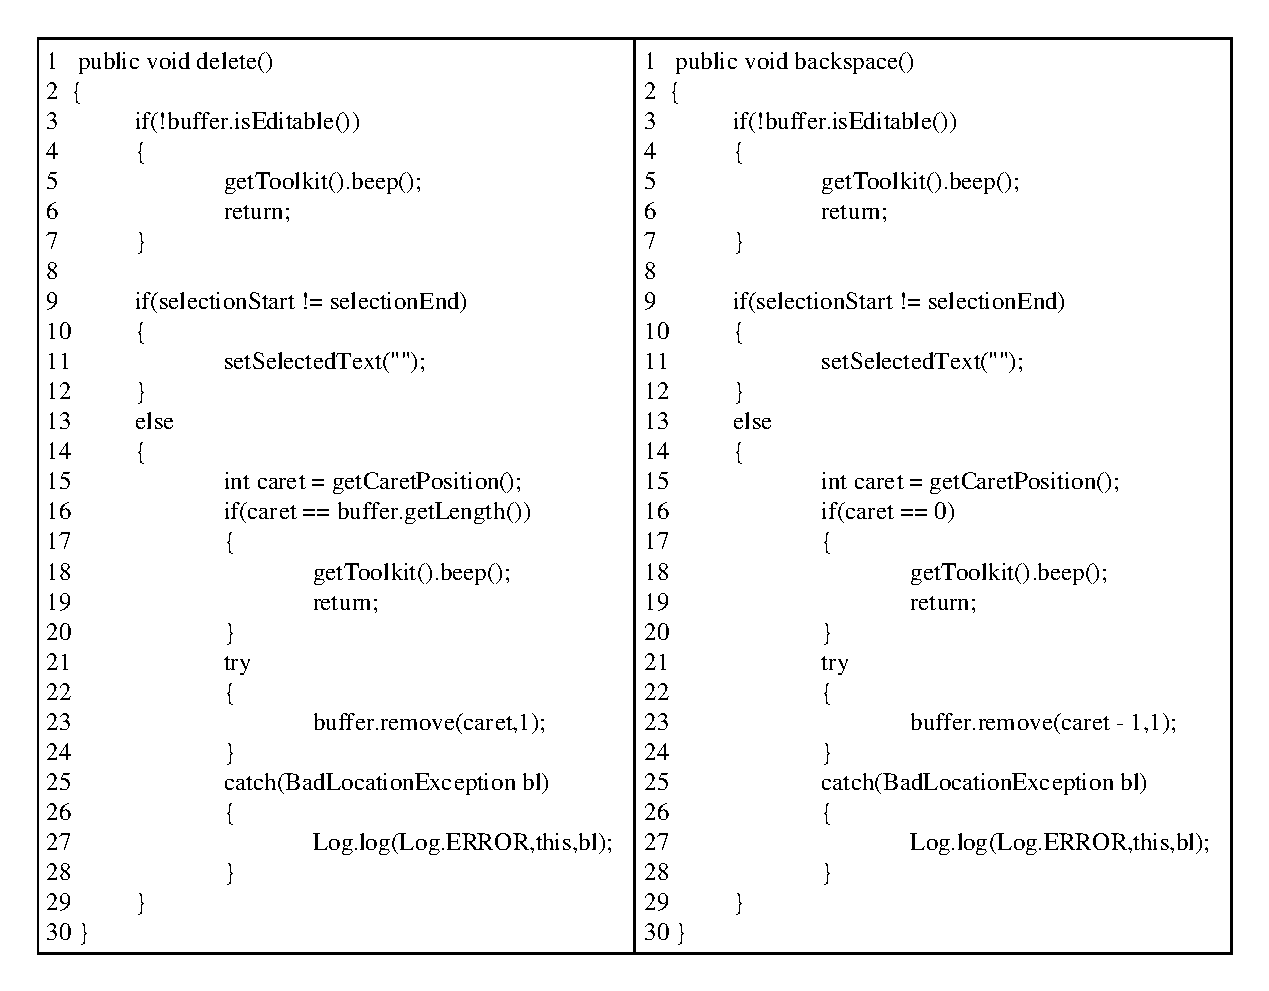
\includegraphics[width=0.8\textwidth]{co-changea.pdf}}}
\subfigure{\label{cg2}}\addtocounter{subfigure}{-2}
\subfigure[Two clone fragments in clone group in version $3.2.0$]
{\subfigure[版本$ 3.2.0 $中克隆组中的两个克隆片段]{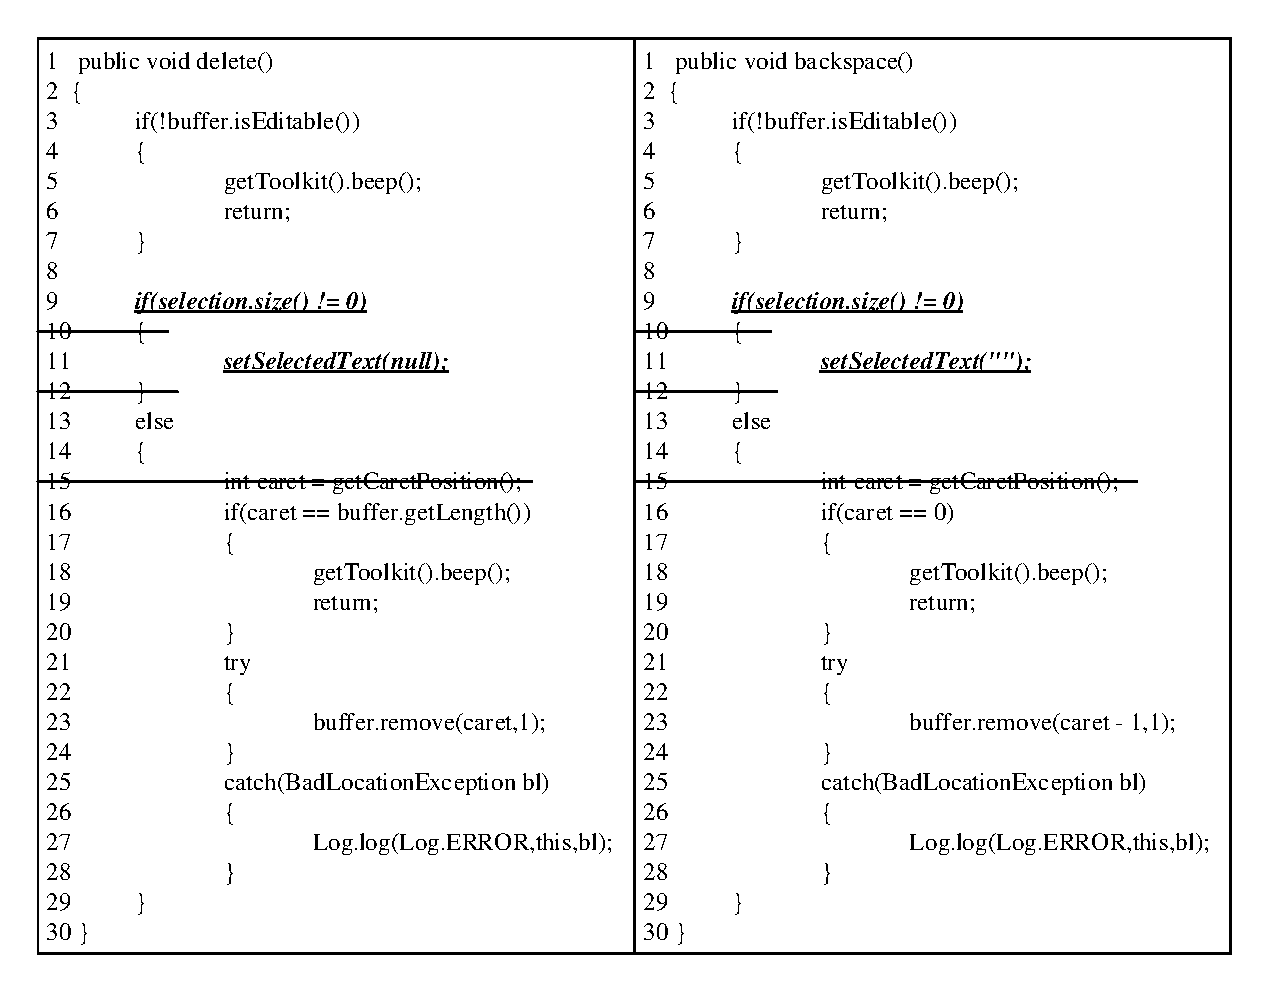
\includegraphics[width=0.8\textwidth]{co-changeb.pdf}}}
\bicaption[co-change]{}{jEdit中的一致性变化的例子}
{Fig.$\!$}{An example of consistent change from jEdit}
\vspace{-1em}
\end{figure}

鉴于此,本章对发生变化的克隆代码进c行一致性预测,在克隆代码变化时,预测克隆代码的一致性维护需求。本章在克隆代码演化的基础上结合克隆代码一致性维护,首先给出了一种克隆代码变化时的一致性变化和一致性维护需求的定义,可以帮助预测克隆变化的一致性维护需求。然后,在第二章研究的基础上重新设计了代码属性、上下文属性和演化属性三组属性表示克隆代码的变化实例。最后,使用贝叶斯网络在克隆代码变化时预测其一致性维护需求。本章方法可以帮助程序开发人员避免克隆一致性缺陷,从而降低克隆代码的一致性维护代价。
%因此,本章方法可可以提高系统的可维护性和软件质量。



%我们通过WEKA \cite{hall2009weka}开发和构建了一个贝叶斯网络作为预测器,并对三个软件项目的预测能力进行了实验。
%我们的实验表明:预测器执行稳定的精确度和召回,对于克隆一致性要求和无一致性的预测,精度范围在70\%到80\%之间,其召回率在63\%和83\%之间。 {\em {我们的实验表明:预测变量的精确度和回忆率对于一致性要求和自由变化实例具有每个存储库的稳定范围;并且为了保持一致性,精度范围在70到80\%之间,其召回率在63和89\%之间。}}此外,每个属性集以其自身的方式对预测能力作出肯定贡献,并且这些属性集中的任何属性集的缺失都可能不利地影响预测器的回忆能力。 {我们的方法可以集成在IDE中以维护克隆更改,这可以避免克隆一致性缺陷。}
%本文的贡献如下:
%\begin {itemize}
%\item 我们提出一种方法来预测克隆组中发生克隆变化所致的一致变化的需要。
%\item 我们基于与克隆系谱相关的信息来识别一组新的属性用于预测。结果表明,这套属性对预测变量的回忆能力有积极影响。
%\item 我们通过对四个开源项目的评估来证明这种预测的可行性。结果表明,我们的方法可以有效预测克隆组的一致变化,具有良好的精度和合理的回忆,并可以帮助提高软件的可靠性通过预测性克隆维护的可重用性。
%\end {itemize}



%在我们的工作中,我们使用克隆检测工具{\em NiCad}来检测来自软件库的克隆。这里,如果两个(或更多个)克隆片段足够相似,则它们形成克隆组。在{\em NiCad}中,这种相似性度量用UPI(代表{\em unique percentage items})表示。UPI根据代码的百分比定义了两个克隆片段之间的{\em 差异}。例如,值为$ 0.3$的UPI表示这两个克隆片段中的30\%不同;换句话说,它们中的70\%具有相同的代码行。
%在这项工作中,{\em  我们设置一个阈值$tau-{CG}$为$0.3$形成克隆组};即,如果UPI $(c_1, c_2)- 0.3$,两个克隆片段$ c_1 $和$ c_2 $被视为属于同一克隆组。}


\BiSubsection{克隆变化时一致性维护需求定义}
{The Definitions for Clone Changing Consistency-Requirement}

在克隆代码的演化过程中,克隆片段可能会被开发人员修改,从而导致克隆代码的一致性变化,这种克隆代码变化可能会导致克隆一致性缺陷。为了描述克隆代码的这种修改,本章给出克隆代码变化时一致性变化定义,如下所示:\\

\begin{definition}
[变化时一致性变化(Changing Consistent Change)]  
\label{def-changingchange}
给定存在两个克隆代码片段 $CF_1$和 $CF_2$,且它们被分别地修改为$CF'_1$和$CF'_2$。  如果对于一个非常小的阈值$\tau$,克隆代码$CF_1$和$CF_2$的变化满足以下条件,称此变化为{克隆变化时的一致性变化(Changing Consistent Change)} , 
  \[
  \begin{array}[t]{crl}
    \mathit{textSim}(CF_i, CF'_i) < 1 & \forall i \in \{1,2\} &(1) \\
    \multicolumn{2}{c}{| ~\mathit{textSim}(CF_1,CF'_1)  ~-~ \mathit{textSim}(CF_2,CF'_2) ~| ~< ~ \tau}  & (2)
  \end{array}
  \]
\end{definition}

%% \ begin {definition} [$ \ tau $ -Conistent change]
%% \ label {defn-1}
%% {\ em
%%假定两个克隆片段$ c_1 $,$ c_2 $分别修改为$ c'_1 $和$ c'_2 $ %%。我们认为$ c_1 $和$ c_2 $之间的修改是$ \ tau $ - {\ em一致的更改\ /}如果对于某个阈值$ \ tau $,
%% \ [
%% \ begin {array} [t] {l}
%% \ mathit {textSim}(c_i,c'_i)<1 ~~~ \ forall i \ in \ {1,2 \} \\
%% | 〜\ mathit {textSim}(c_1,c'_1)〜| 〜 - 〜|〜\ mathit {textSim}(c_2,c'_2)〜| 〜<〜\ tau
%% \ end {array}
%% \]
%%}
%%注意$ \ mathit {textSim} $是根据NiCad中使用的%%度量实现的相似性度量。 \ textcolor {blue} {在NiCad中,这种相似性度量是以UPI(代表{\ em唯一百分比项目})表示的%%。}
%% \ end {definition}
%% 
  
注意$\mathit {textSim}(c,c')= $ 1 - UPI($ c,c'$),UPI是两个代码片段之间不同的代码行数占总代码行的比例,计算方式同第二章中的计算方式相同。第一个约束条件要求 $ CF_1 $和$CF_2 $同时修改;第二个约束条要求$ CF_1 $和$CF_2$发生满足阈值$\tau$条件下一致性的变化,即对代码片段进行了非常相似且一致的变化。本章中$\tau$取值为$0.003$,要求代码片段之间变化完全一致。

变化时一致性变化,不仅要求克隆代码片段被同时修改,还要求一致的变化。原因在于:在克隆代码变化时,目的是避免克隆变化可能导致的未来演化中的一致性变化,及其因此所引发的克隆一致性缺陷。因此, 不仅要求两个克隆代码片段同时变化,还需要发生相似的变化,否则将会引入克隆一致性缺陷。

在克隆演化过程中,克隆片段的变化必然也会导致克隆组的变化,而克隆组的变化可以使用克隆演化模式进行描述,即一致性变化模式。本文给出演化过程中克隆组的一致性变化模式定义,如下所示:\\

\begin{definition}
[变化时一致性变化模式( Changing Consistent Change Pattern)] 
\label{def-changingpattern}
在软件版本 $j+1$中存在一个克隆组$CG'$ ,假设克隆组内至少存在两个克隆代码片段$CF'_1$ 和 $CF'_2$可以与映射到上一版本$j$的克隆组$CG$中,且 $CG$中与之对应的克隆代码片段的 $(CF_1,CF_2)$被修改为$(CF'_1,CF'_2)$。如果克隆片段之间的变化( $(CF_1,CF_2)$变化至$(CF'_1,CF'_2)$满足克隆片段的“一致性变化(Consistent Change)”,则称克隆组$CG'$具有一致性变化模式(Consistent Change Pattern)。
\end{definition}

%\begin{definition}[{\bf Consistent/Inconsistent Change Pattern}] 
%  \label{}
%  {\em 
%  Given a threshold $\tau$. A clone group $G'$ in software version $j+1$ possesses {\em\bf consistent change pattern} if there exists a pair of clones $c'_1,$ and $c'_2$  in $G'$ which are mappable to a pair of clones $c_1$ and $c_2$ in a clone group $G$ in version $j$ such that modification of code pairs from $(c_1,c_2)$ to $(c'_1,c'_2)$ is a $\tau$-consistent change. Conversely, we say that clone group $G'$ in version $j+1$ possesses {\em\bf inconsistent change pattern}.
%  } 
%\end{definition}

变化时的一致性变化模式,与其它论文中使用的定义不同,其原因在于:本章目的在于预测克隆代码的一致性所导致的克隆一致性缺陷。为了便于读者更容易理解克隆变化时的一致性维护需求,本章现给出克隆变化实例的定义,如下所示:\\

%Definition~\ref{defn-2} differs from those used in the earlier work such as \cite{Kim2005,Saha2011}, which identify consistent change by asserting that {\em all} clones evolving from previous version of clone group are detected to be similar by clone detection tools.
%More importantly, we label a clone group with consistent change pattern {\em so long as consistent change (as defined above) occurs for a pair of clones.\/} 
%We believe this definition aligns better with the understanding that as long as there exists a pair of clones that needs consistent change, we should inspect the clones in the clone group when any clone has been modified.
%Consequently, the clone genealogy that we build will be different from that of \cite{Kim2005,Saha2011}. 

\begin{definition}
[克隆变化实例( Clone Changing Instance)] 
\label{def-changinginstance}
克隆变化实例:
软件版本 $j$中的一个克隆组$CG$是克隆变化实例,如果克隆组$CG$中至少两个克隆代码片段发生变化,且版本$j+1$ 中至少存在一个克隆组$CG'$与之对应(在同一克隆家系$CGE$中)。 
\end{definition}

%\begin{definition}[{\bf Change Instance}] 
%\label{}
%{\em 
%A clone group $G$ in version $j$ is a {\bf change instance} if at least one clone group $G'$ in version $j+1$ which is connected to $G$ in the clone genealogy possess consistent or inconsistent change pattern. 
%}
%\end{definition}


给定一个克隆变化实例,在其未来的演化过程中,可能会导致克隆组的一致性变化模式。克隆组的一致性变化可能会导致一致性缺陷,从而降低软件质量。因此,在克隆代码变化时,预测其未来演化过程中是否会发生一致性变化,可以避免由克隆变化实例导致的一致性缺陷。本文将克隆变化所导致的一致性变化,称为克隆一致性维护需求。克隆变化时的一致性维护需求定义如下:\\
%接下来,虽然一致和不一致的更改模式指定克隆如何从一个版本发展到下一个版本,但我们实际上更有兴趣了解一对克隆{\em 是否会在未来}中发生一致的更改。这是因为在实践中,开发人员可能选择延迟做出一致的更改,或者有时他们可能甚至不知道需要进行一致的更改,直到未来出现问题.

\begin{definition}
[变化时一致性维护需求(Changing Consistency-Requirement)] 
 \label{def-changingrequirement}
给定版本 $j$中一个克隆变化实例,$CG$满足克隆一致性维护需求(Consistency-Requirement),如果在版本$k$中存在一个克隆实例 $CG'$($k>j$)满足以下条件: (1) 在$CG'$中至少存在两个克隆片段在其克隆家系$CGE$中可以映射到克隆实例 $CG$中, (2) $CG'$ 具有“一致性变化模式”(Consistent Change Pattern)。反之,假如克隆变化实例$CG$ 不满足克隆一致性维护需求条件,称该克隆实例不需要一致性维护(consistency-requirement free,或者consistency-free)。
\end{definition}

%\begin{definition}[{\bf Consistency-Requirement (Free)}] 
%  \label{}
%  {\em 
%A change instance $G$ in software version $j$ satisfies 
%{\bf  consistency-requirement\/} condition if there is a clone group $G'$ in software version $k$, with $k>j$, such that (1) there is at least a pair of clones in $G'$ that is mappable in clone genealogy to a pair of clones in $G$, and (2) $G'$ possesses ``consistent change pattern''. 
%When $G$ does not satisfy consistency-requirement, we say that it is {\bf  consistency-requirement free\/}, or simply {\em consistency-free\/} for short. }
%\end{definition}

最终,可以将本章的的研究问题表述如下:给定一个克隆变化实例,即克隆组中$CG$的克隆代码片段$CF$被修改,确定$CG $是否满足克隆变化时一致性维护需求。

更进一步,根据上述定义克隆变化实例只有两种状态:满足和不满足一致性维护需求。我们将变化实例的一致性要求的预测转化为分类问题。本章克隆变化时的克隆一致性需求预测问题可转换为一个典型的分类问题,因此使用机器学习模型解决此分类问题,具体方法见下文。

\BiSection{克隆变化时一致性维护需求预测框架} 
{The Framework of Clone Changing Consistency-Requirement}

为解决本章所提出的克隆一致性需求维护预测问题,本文首先给出了一个方法框架。
基于贝叶斯网络的克隆变化时一致性维护需求预测框架架如图~\ref{framwork3}所示。方法可以划分为三个阶段,克隆变化实例收集阶段、克隆变化实例表示阶段和一致性维护需求预测阶段。收集阶段旨在收集系统中全部的克隆变化实例,可将其用于使用机器学习方法中来训练预测模型。由于实际的克隆变化实例无法直接应用于机器学习方法中,因此在表示步骤中将提取相应的属性值表示克隆变化实例。接下来,在预测步骤,使用属性化的克隆变化实例构建和训练机器学习模型,并使用其预测克隆变化实例的克隆一致性维护需求。

\begin{figure}[htbp]
\centering
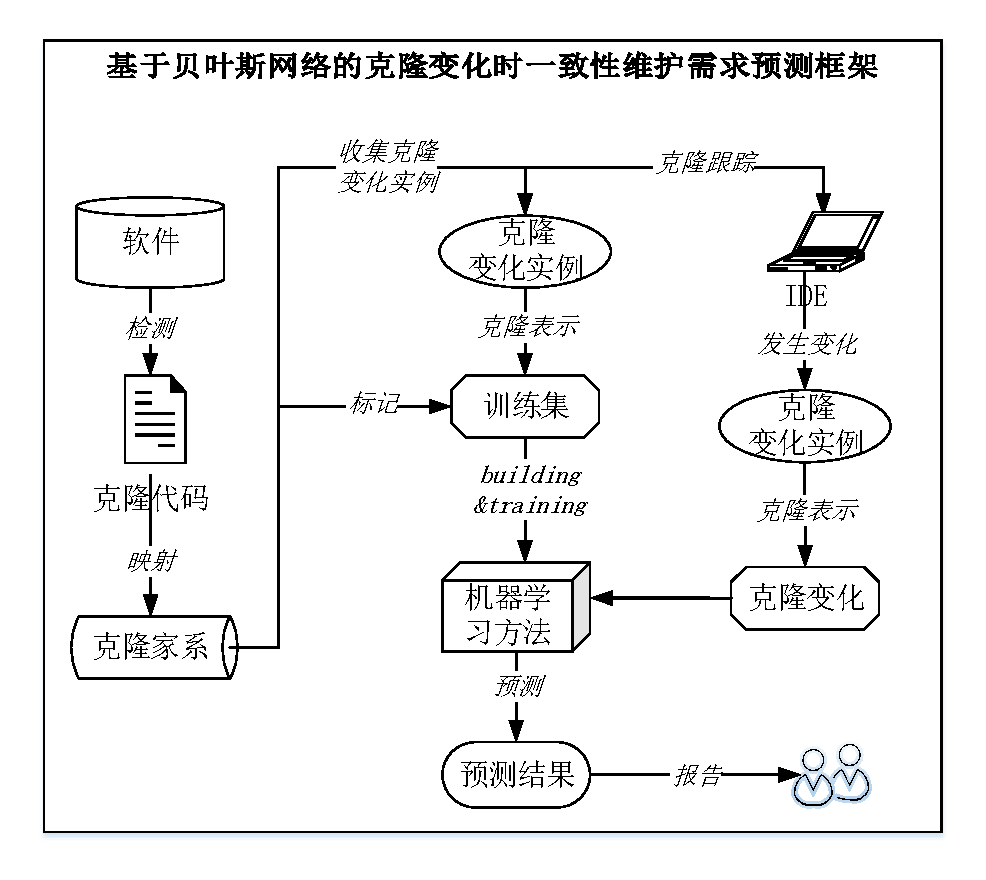
\includegraphics[width = 0.8\textwidth]{framework4.pdf}
\bicaption[framework4]{}{基于贝叶斯网络的克隆变化时一致性维护需求预测框架}
{Fig.$\!$}{The framework for clone changing consistency prediction based on Bayesian network}
\vspace{-1em}
\end{figure}

具体来说,在收集阶段中,通过构建系统的克隆家系从软件中收集所有的克隆变化实例。使用NiCad来检测软件版本中的所有克隆,并通过在相邻版本的克隆组之间进行映射来构建克隆家系,用于识别克隆变化实例。在表示阶段中,通过提取属性值表示克隆变化实例,提取了代码属性、上下文属性和历史属性三组属性组,同时,还提取了关于克隆变化的相关信息。在预测阶段中,使用收集到的克隆变化实例训练贝叶斯网络,并在克隆变化时预测克隆一致性维护需求。在使用已构建好的模型进行预测时,可将该模型嵌入到软件开发环境中。软件开发环境需要实时跟踪克隆代码的变化(克隆变化实例),然后提取克隆变化实例的度量值。最后,使用模型预测其一致性维护需求,根据预测结果提醒程序开发人员采取进一步的维护操作。

克隆变化实例有两种不同的预测结果,即满足一致性维护需求和不满足维护需求。对于满足一致性维护需求实例来说,其在将来的演化中可能会引发一致性变化,程序开发人员需要验证克隆组内克隆代码的一致性问题。对于不满足一致性维护需求实例来说,其在将来的演化中不会引发一致性变化,程序开发人员可以放心的对该克隆代码进行修改,不必考虑克隆一致性问题。

本章基于贝叶斯网络预测克隆变化实例的一致性。使用克隆变化实例属性表示贝叶斯网络中的节点,并用于构造贝叶斯网络的结构。使用收集到的克隆变化实例学习贝叶斯网络的参数,从而完成模型的训练,细节可参考本文后续章节。

\BiSection{收集克隆变化实例}
{Collecting Clone Changing Instance}

收集克隆变化的的目的在于生成克隆一致性预测的训练集,并将其用于训练机器学习模型。通过构建系统的克隆家系并识别其中的克隆演化模式,可以从软件中收集所有的克隆变化实例。首先使用NiCad来检测软件版本中的所有克隆,然后通过在相邻版本的克隆组之间进行映射来构建克隆家系,最后识别克隆一致性演化模式识别系统中的克隆变化实例。

根据定义~\ref{def-changinginstance}~,本文假定克隆家系$CGE$中发生变化的克隆组为克隆变化实例。因此通过构建克隆家系并识别克隆家系中发生变化的克隆组,可以收集克隆创建实例。

(1)构建克隆家系。首先,下载系统所有版本的源代码,并使用NiCad的默认配置检测检测每一版本的中Type1-3的克隆代码。然后,通过映射所有相邻版本的克隆代码,构建系统中全部克隆家系。为完成版本间的映射,为每个克隆片段生成一个克隆区域描述符 $CRD$\cite{duala2010clone},使用基于CRD的克隆映射算法映射两个连续版本之间的所有克隆片段和克隆组\cite{ci2013new}\cite{ci2013newD}。根据克隆映射结果,构建系统的克隆家系。

(2)识别克隆演化模式和收集克隆变化实例。首先,识别克隆家系中的克隆演化模式。构建克隆家系后,通过对比相邻版本的克隆代码,可以识别克隆家系的克隆演化模式,尤其是一致性变化模式(参考定义~\ref{def-evolutionpattern}~和\ref{def-changingpattern}~)。所识别的克隆演化模式有三个作用:(a)可以用于表示克隆变化实例,本文使用克隆演化模式作为表示克隆变化实例的部分演化属性。因此,克隆演化模式可以用于克隆变化实例表示中。(b)克隆演化模式可以帮助收集克隆变化实例。根据定义~\ref{def-changingchange}~可以识别系统中发生一致性变化的克隆代码和克隆组,从而确定克隆家系中的克隆变化实例。(c)克隆演化模式可以帮助确认克隆一致性维护需求。根据定义~\ref{def-changingrequirement}~,一致性维护需求,可以通过遍历克隆家系$CGE$是否发生了一致性变化模式(定义~\ref{def-changingpattern}~)进行确定。

然后,收集克隆变化实例。在识别克隆家系演化模式,尤其是一致性变化模式后(~\ref{def-changingpattern}~),根据定义~\ref{def-changinginstance}通过识别克隆家系中的变化克隆组,便可以收集系统中的克隆变化实例。

(3)标识克隆变化实例的一致性维护需求。在收集所有的克隆变化实例后,还需确认相关实例的一致性需求。根据定义~\ref{def-changingchange}~和~\ref{def-cloningrequirement}~,通过遍历克隆变化实例所在的克隆家系$CGE$的演化情况,确定其一致性维护需求。如果克隆变化实例在其演化过程中发生了一致性变化模式(~\ref{def-changingpattern}~),则该实例满足一致性维护需求,否则不满足维护需求。

\BiSection{克隆变化实例表示}
{Representing of Clone Changing Instance}

%由于实际的克隆变化实例无法直接应用于机器学习方法中,因此在表示步骤中将提取相应的属性值表示克隆变化实例。在表示阶段中,通过提取属性值表示克隆变化实例,提取了代码属性、上下文属性和历史属性三组属性组,同时,还提取了关于克隆变化的相关信息。

在模型训练中,每个变化实例由它们表示属性。我们从每个克隆实例中选择了三组属性作为贝叶斯网络模型的输入。这三组捕获克隆组的三个不同方面。它们是代码属性,上下文属性和进化属性。
前两组与Wang等人提供的类似。 \cite{} {Wang2014},而最后一个属性集是新添加的,旨在捕获克隆进化属性。

(1){Code attributes}
这些属性捕获组中代码克隆的特征。属性类似于\cite{} {Wang2012}中收集的属性。主要区别在于它们的计算:Wang et al。 从两个代码聚集的属性:复制和粘贴代码。这里,我们计算每个属性的平均值,当需要时。因此,我们的属性包括代码行的平均数,参数的平均数,调用调用的平均数。此外,我们有:

\begin{itemize}
\item Clone Group Size: 
The number of code fragments in the clone group.
%% \item Average Code Lines: The average number of code lines for all
%%  clone fragments in clone group.
\item Average Number of Halstead: 
The average number of Halstead for all clone fragments in clone group. The Halstead includes the number of distinct operators, number of distinct operands, total number of operators, total number of operands.
%% \item Average Number of Parameters: The average number of parameters
%%   for all clone fragments in the clone group.
\item Average Number of Important Syntactic Constructs: 
For each important syntactic construct (such as \verb+if+, \verb+while+, etc.), we compute the average number of occurrences of the construct for all clone fragments of clone group.
%% \item Average Number of Invocations: The average number of method
%%   invocations for all clone fragments in the clone group, which
%%   includes all invocations, library invocations, local invocations,
%%   and other invocations.
\end{itemize}

(2)Context attributes

该集合包含克隆组中克隆的上下文信息,其中一些类似于Wang等人收集的那些。 在\cite{} {Wang2012}中,主要的区别在于我们计算克隆组中的值,而不仅仅是两个克隆。此外,我们添加了几个属性来描述克隆上下文,例如克隆相似性,参数类型和块信息等。这里是属性列表:

\begin{itemize}

\item Average Clone Similarity: 
The average similarity value between each pair of clones in the clone group. 

\item Locality of Clones: 
This flag determines if all the clone fragments reside in the same file. 

\item Average File Name Similarity : 
There are two attributes to average file name similarity: the real similarity and the masked similarity. 
The mask similarity is a flag indicating if all clones exist in one file. 
In the case when not all the clones are in one file, the real similarity is the average of the similarity measure between the names of the files containing clones. 
Here, Levenshtein distance-based similarity \cite{Navarro2001} is used. 
  
\item Average Method Name Similarity: 
This is the average of the similarity between the names of the methods in which a clone in the clone group belongs.

\item Average Sum of Parameter Similarity (ASPS): 
First, we compute the ``sum of parameter similarity'' (SPS) for each clone pair in the group, as follows: Let $M_1$ and $M_2$ be the two clones with parameters ($P_1$, $P_2$, $\ldots$, $P_m$) and ($Q_1$, $Q_2$, $\ldots$, $Q_n$) respectively. 
We define SPS to be: $\sum_{i=1}^{m}\sum_{j=1}^{n} \mathit{Sim}(P_i,Q_j)$. 
The final ASPS is the average of SPS's.

\item Average Sum of Parameter Type Similarity (ASPTS): 
Similar to ASPS measurement, but applying to parameter type names.

\item Average Maximal of Parameter Similarity (AMPS): 
For each pair of clones $pc$, we compute the {\em maximal of parameter similarity (MPS)}, which is defined as: $\mathit{Max}(\mathit{Sim}(P_i,Q_j))$, where $1\leq i\leq m$, $1\leq j\leq n$, and $\mathit{Sim}(x, y)$ denotes the similarity between string $x$ and string $y$. 
The final AMPS is the average of these MPS's. 

\item ``Is-same-block'' Flag:  
This flag indicates if all the clones are enclosed within block statements of the same syntax.
\end{itemize}

(3)Evolution attributes

最后一组包含关于家谱的属性。克隆组的特征,并且它涉及克隆组如何演变为当前版本。在整个进化历史中,对于一些修订可以存在变化实例,并且还可以经历多于一个变化。这些可以从克隆系谱中提取。 属性是:
  %对于这些指标,我们使用克隆生命周期,其生命周期中的克隆模式数量作为指标:
  %

\begin{itemize}
\item Clone Group Age: 
The number of versions the clone group has existed in this repository until now.

\item Number of Clone Patterns: 
The number of clone patterns which this clone group experiences until now since its inception. 
For each clone pattern, we determine the number of occurrences of this pattern in the clone group's history.

\item Current Pattern: 
The clone pattern of this clone group, as derived from its change (or unchanged) from the previous version (as formally specified in Definition~\ref{defn-2}.)

\item Summaries of Clone Changes: 
The number of changes of this clone group since its inception until the current version.
For each important code syntax (as specified in the set of code attributes), we capture two pieces of information: We summarize the number of times in the clone genealogy (till the present version) that the syntax experiences an increase (and decrease) in its value from one version to the next immediate version. 
For instance, suppose that from the clone genealogy, we discover that a clone group originates in version $i$, and evolves till current version $j$ (where $j > i$). 
We then compare the {\em changes} in the average number of \verb+if+ statements (one of the clone attributes) between two successive versions: versions $i$ and $i+1$, $\cdots$, versions  $j-1$ and $j$. 
This returns to us a series containing positive and negative numbers.
We then record the total number of positives and negatives, forming two summaries associated with \verb+if+statements.
\end{itemize}

\noindent
{\bf Change information.} 
对于每个更改实例,我们还收集有关更改实例中对克隆进行的更改的信息,当它从当前版本发展到下一个版本时。

\begin{itemize}
\item Current Clone Change: 
The change of this clone group from the current version to the immediate next.  
We capture this change for each important syntactic construct.
\end{itemize}

\BiSection {训练与预测}
{Training and Predicting} 

%接下来,在预测步骤,使用属性化的克隆变化实例构建和训练机器学习模型,并使用其预测克隆变化实例的克隆一致性维护需求。在预测阶段中,使用收集到的克隆变化实例训练贝叶斯网络,并在克隆变化时预测克隆一致性维护需求。在使用已构建好的模型进行预测时,可将该模型嵌入到软件开发环境中。软件开发环境需要实时跟踪克隆代码的变化(克隆变化实例),然后提取克隆变化实例的度量值。最后,使用模型预测其一致性维护需求,根据预测结果提醒程序开发人员采取进一步的维护操作。

\BiSubsection {训练}
{Training} 
对于每个主题知识库,我们通过收集其变化实例的属性来构建训练数据集。所需的最后一个准备工作是与每个实例关联其一致性 - 要求/无一致性指示,如定义~\ref{defn-4}~中定义。 其中一些将用于训练模型,其他将被用作预测验证的基础真理。最后,形成的数据集将提供给WEKA以开发用于预测的贝叶斯网络模型。在训练模型中,贝叶斯网络的节点表示属性,边缘是属性之间的条件依赖性。



我们应用贝叶斯网络学习技术来解决它。
贝叶斯网络是表示一组随机事件及其条件依赖性的概率图形模型。
形式上,它是一个有向的非循环图,使得其节点表示随机事件,其边缘表示两个节点(事件)之间的条件依赖关系。不连接的两个节点表示有条件地彼此独立的两个事件。
与每个节点相关联的是概率函数,其根据与节点父事件相关联的值计算由节点表示的事件的概率。
有关详细信息,请参阅热门读者\ cite {Pearl1985}



%We apply Bayesian network learning technique to address it. 
%A Bayesian network is a probabilistic graphical model representing a set of random events and their conditional dependencies. 
%Formally, it is a directed acyclic graph such that its nodes represent random events, and its edges represent conditional dependencies between two nodes (events); Two nodes which are not connected represent two events that are conditionally independent of each other.
%Associated with each node is a probability function that computes the probability of the event represented by the node from the values associated with the nodes parent events. 
%We refer avid readers to \cite{Pearl1985} for details.

\BiSubsection {预测}
{Predicting} 
在此步骤中,当现有克隆组发生更改时,软件维护人员可以使用我们的预测变量来预测克隆一致性。如图~\ref{}~所示,我们的方法可以集成到一个IDE,如eclipse,可以保持克隆在开发阶段的变化。运行预测变量需要跟踪克隆在软件进化及其变化中的支持。一旦检测到克隆更改,该工具将提取与此更改实例相关的所有属性,预测其一致性要求,并通知开发人员。
根据预测,开发者因此可以根据需要一致地保持克隆。

这需要IDE提供两个基本功能。第一个功能要求开发人员跟踪克隆及其关联的克隆组,第二个功能需要IDE监控克隆的更改。当开发人员可以跟踪和监视代码克隆时,预测变量可以预测克隆发生变化时一致性要求的可能性。 {\emph {跟踪克隆和监控克隆更改}。首先,我们跟踪克隆及其在IDE中的更改。 \underline {CRD的方法}可以应用于跟踪克隆及其更改。 \emph {提取更改克隆属性和预测一致性要求。}当克隆发生更改时,我们从其关联的克隆组中提取属性。之后,我们将这些数据放入我们的训练模型中,以预测这种一致性要求。 \emph {向开发人员发出警告信号}。我们的预测器将提供描述此更改实例需要一致性要求的概率的分数(介于0和1之间)。这将有助于开发人员考虑是否更改同一组中的克隆。

\BiSection{实验结果和分析}
{EXPERIMENTS}

\BiSubsection{实验设置}
{Methodology}

我们对四个开源的仓库进行了实验项目。表~\ref {}提供了这些项目的详细信息。从表中可以看出,每个项目有数百个更改实例,范围从159到1040个,项目{\em  jEdit}是最小的存储库。其中,满足一致性要求(即,导致克隆组在未来一致的改变)的改变实例的数量显示在列3中,而列2反映了一致性要求自由的改变实例的数量 ,do {\em not }导致任何一致的更改)。
更改满足一致性要求的实例需占用33\%\~\% 5\%到74 \%的所有更改实例。

\begin{table}[htbp]
\bicaption[wdwfas1]{}{符合研究生院绘图规范的表格}{Table$\!$}{The four open source projects for experiment}
\vspace{0.5em}\centering\wuhao
\begin{tabular}{cccc}
\toprule[1.5pt]
~\multirow{3}{*}{\textbf{Project}}& \multicolumn{2}{c}{\textbf{Number (Percentage) of Change Instances}} & \multirow{3}{*}{\textbf{Total}}\\ 
 \cline{2-3}
 ~& \textbf{Consistency-} &\textbf{Meeting} & ~\\
 &\textbf{Requirement Free}&\textbf{Consistency-Requirement}&\\
\midrule[1pt]
ArgoUML&288(67.45\%)&139(32.55\%)&427\\
jEdit&78(49.06\%)&81(50.94\%)&159\\
jFreeChart&452(43.46\%)&588(56.54\%)&1040\\
Tuxguitar&91(25.71\%)&263(74.29\%)&354\\
\bottomrule[1.5pt]
\end{tabular}
\end{table}

%表~\ ref{}~显示从三个项目收集的变更实例的大小的统计信息。中间列显示收集的至少一半的更改实例的大小为2。因此,虽然克隆是丰富的,但它们对系统的引入并不猖獗。{\em  ArgoUML}和{\em jFreeChart}确实有一些超大克隆组; 这些预期在数量上是小的,并且克隆的尺寸也小。

%\begin{table}[htbp]
%\bicaption[table1]{}{符合研究生院绘图规范的表格}{Table$\!$}{Statistics of the size of clone change instances}
%\vspace{0.5em}\centering\wuhao
%\begin{tabular}{ccccc}
%\toprule[1.5pt]
%\textbf{Project}&\textbf{Total}&\textbf{Mean}&\textbf{Standard Deviation}&\textbf{Median}\\ \hline
%\midrule[1pt]
%ArgoUML&427&7.5.9271&	26.22377&2\\ \hline
%jEdit&159&	2.46541&	0.9125&2\\ \hline
%jFreeChart&1040&	7.85288&	26.92378&2\\ \hline
%Tuxguitar&354&	3.40395	&3.45232&2\\ 
%\bottomrule[1.5pt]
%\end{tabular}
%\end{table}

%表~\ref{}描述了更改实例的年龄的统计信息。如前所述,变更实例的年龄是自成立以来所经历的软件版本控制的数量(从$ 0 $计算)。一般来说,更改实例的年龄较小。考虑到变更实例的性质,他们将在当前版本中进行一些代码更改,这个统计数据显示大多数克隆组开始在早期体验代码更改。因此,我们尽可能早地执行一致性要求可满足性的预测变得更相关。

%\begin{table}[htbp]
%\bicaption[dffhg1]{}{符合研究生院绘图规范的表格}{Table$\!$}{Statistics on ages of clone change instances}
%\vspace{0.5em}\centering\wuhao
%\begin{tabular}{ccccc}
%\toprule[1.5pt]
%\textbf{Project}&\textbf{Total}&\textbf{Mean}&\textbf{Standard Deviation}&\textbf{Median}\\ \hline
%\midrule[1pt]
%ArgoUML&427&2.09368&2.33078&1\\ \hline
%jEdit&159&4.48428&3.64371&3\\ \hline	
%jFreeChart&1040&4.93462&4.99543&3\\ \hline	
%Tuxguitar&354&1.5565&1.50294&1\\ \hline	
%\bottomrule[1.5pt]
%\end{tabular}
%\end{table}

我们使用WEKA包建立和培训贝叶斯网络预测模型。WEKA是一个非常灵活和易于使用的数据挖掘工具,包含几种分类/预测方法。在构建我们的模型中,我们选择{\em K2}用于学习网络结构的算法,并且一旦结构已经被学习,使用{\em  SimpleEstimator}来估计贝叶斯网络的条件概率表。贝叶斯网络中的父节点的最大数目被设置为$ 4 $,以便适应属性之间的可能的依赖性,同时不过度消耗模型构造所需的过多的存储器和时间。对于每个克隆更改实例,模型将输出一个值,即其{\em consistency-requirement}的概率。接近$ 1 $的概率值意味着由改变实例经历的当前改变满足{\em consistency-requirement}准则的可能性很高。另一方面,更接近$ 0 $的值意味着这个变化实例很可能是{\em consistency-requirement free}。

基于推断的概率,我们的实验可以自然分为两部分:满足一致性要求和满足无一致性。对于满足一致性要求的更改实例,我们使用{\em Waring Rate,Precision和Recall}来评估我们的方法,该方法尝试警告开发人员可能有一致的更改。另一方面,我们使用{\em Recommendation Rate,Precision and Recall},当克隆变化被推断为无一致性时,尝试推荐开发人员自由地进行任何改变,具有高概率。这些标准的定义在接下来的两个小节中描述。

类似于\cite{} {Wang2012}中的工作,我们从三个不同的角度评估我们的预测的质量。首先,{\em 有效性实验}:我们利用从三个项目中的每一个提取的所有属性来训练和测试模型,并评估预测的质量。第二,{\em 属性集实验}:我们评估三个贡献属性集中的每一个对预测质量的影响。最后,{\em 跨项目实验}:当使用从其他项目提取的数据构建预测模型时,我们评估项目的预测质量。

%我们在具有Intel(R)Core(TM)i5-4210M CPU @ 2.60GHz和8G RAM的桌面上运行我们的实验。每个实验花费不到一分钟的模型构建,交叉验证少于5分钟。大多数实验时间花费在数据准备,包括家谱建构和克隆变化实例收集,其范围在5至30分钟之间。然而,我们注意到,在实践中,克隆系谱构建和变更实例收集将逐步执行,随着软件发展到新版本。因此,数据准备的开销将不是实际问题。

\BiSubsection{一致性实验}
{Consistency-Requirement Experiment}

在本实验中,我们计算以下三个指标来评估我们的模型的一致性要求的可预测性:
\begin{itemize}
\item \textbf{Warning Rate (WR)}: 
This percentage indicates the number of change instances that our model predicts to have met consistency-requirement, and thus warns developers to check for possible consistent change.
It is computed as the ratio of the number of warning raised by the model to all change instances tested. 

\item \textbf{Precision}: 
This assesses the accuracy of the model when it predicts that a change instance under test meets the consistency requirement. 
It is computed as the ratio of the number of {\em correct} predictions of change instances meeting consistency-requirement to the number of predictions made by the model about change instances meeting consistency-requirement.

\item \textbf{Recall}: 
This assesses the effectiveness of the model in discovering all change instances meeting consistency-requirement.
It is computed as the ratio of the number of {\em correct} predictions of change instances meeting consistency-requirement to total number of change instances meeting consistency-requirement (i.e., ground truth).
\end{itemize}

\BiSubsubsection{全属性组实验}
{Effectiveness Experiment}

在这个实验中,我们为四个项目中的每一个构建不同的模型。每当模型预测变化实例满足一致性要求时,它也提供关于该预测的有效性的概率。 因此,我们可以对该概率值设置阈值,使得我们接受该预测是有效的(仅当相关联的概率值至少等于阈值时)。在这种情况下,模型将认为测试中的变更实例满足一致性要求,并向开发人员发出警告。

因此,我们将阈值设置为不同的值来研究它对预测有效性的影响。阈值设置从0.9到0.5,表~\ref{}描述了我们对三个软件的预测的有效性存储库。表中的每一行指示在特定阈值下的预测的质量。此外,我们使用交叉验证$ 10 $ -folds来训练和测试我们的预测变量。

\begin{table}[htbp]
\bicaption[table1]{}{符合研究生院绘图规范的表格}{Table$\!$}{EFFECTIVENESS OF PREDICTORS ON Four OPEN SOURCE PROJECTS}
\vspace{0.5em}\centering\wuhao
\begin{tabular}{ccccc}
\toprule[1.5pt]
\textbf{Project}&\textbf{Threshold}&\textbf{WR(\%)}&\textbf{Precision(\%)}&\textbf{Recall(\%)}\\

\midrule[1pt]
 \multirow{5}{*}{ArgoUML}
&0.9&	20.14&	69.77&	43.17\\
&0.8&	21.31&	68.13&	44.60\\
&0.7&	24.12&	65.05&	48.20\\
&0.6&	24.59&	63.81&	48.20\\
&0.5&	25.29&	62.04&	48.20\\
\hline
\multirow{5}{*}{jEdit}
&0.9&	43.40&	73.91&	62.96\\
&0.8&	47.17&	70.67&	65.43\\
&0.7&	49.06&	70.51&	67.90\\
&0.6&	50.31&	70.00&	69.14\\
&0.5&	50.94&	69.14&	69.14\\
\hline
\multirow{5}{*}{jFreeChart}
&0.9&	52.50&	82.05&	76.19\\
&0.8&	55.19&	81.36&	79.42\\
&0.7&	56.83&	80.71&	81.12\\
&0.6&	58.65&	80.33&	83.33\\
&0.5&	60.10&	79.68&	84.69\\
\hline
\multirow{5}{*}{Tuxguitar}
&0.9	&76.55&   80.44&	82.89\\
&0.8	&78.53&	80.22&	84.79\\
&0.7	&80.51&	80.00&	86.69\\
&0.6	&81.64&	79.24&	87.07\\
&0.5    &83.33&	79.32&	88.97\\
\bottomrule[1.5pt]
\end{tabular}
\end{table}

创建的模型在预测项目{\em jFreeChart}和{\em Tuxguitar}的一致性要求满足方面非常有效,其中预测的精确度和回忆在80\%左右悬停。它执行相当不错,虽然不是那么好,对于{\em jEdit}资源库。这可能是因为存储库的规模较小,但需要进一步调查。尽管{\em  ArgoUML}没有像其他存储库一样的良好预测,但它仍然可以预测精度在65\%左右的需求,并回忆在45\%左右。对于所有的项目,我们的模型产生了相当合理的警告率;它围绕满足一致性要求的变更实例的百分比(如表~\ ref {}~中所列)。

虽然阈值的变化确实影响精度和召回,它对召回的影响比对精度。这意味着,创建的模型在提供中相当稳定,但可以进一步改进其回忆能力。这意味着开发人员可以非常自信地依赖于预测变量的警告,但可能需要其他方法来帮助进一步识别预测变量保持沉默的情况。一个简单的改进是建立模型以预测和警告一致性无需要求的更改实例,从而减少更改实例的数量,没有任何警告(如Wang等人在\cite{}{Wang2014}中所做的)。然而,仍需进一步调查以提高召回率。

\BiSubsubsection{属性组实验}
{Attribute Set Experiment}

本实验是为了确定三者的影响而进行的属性集对训练模型的预测能力。我们对相同的软件存储库进行了实验,但{\em 排除了每个实验的三个属性集合。}表~\ ref{}~显示分别剥离代码属性,上下文属性和进化属性的结果。然后将这些结果中的每一个与具有存在的所有属性(列3至5)获得的结果进行比较。

正如上面的文章,我们使用{三组属性}来预测一致性 - 退休。 为了研究属性组的贡献,我们分别删除每个组(除了当前的变化),其命名为:{\em without code,without context,without evolution}。 我们不会删除当前的更改,因为我们将使用此更改来预测每个实验的一致性要求。 对于每个实验,我们固定阈值从0.9到0.5,并查看精度和回忆如何变化。 我们还使用WEKA来评估我们的预测与10折交叉验证。

\begin{table}[htbp]
\bicaption[table1]{}{符合研究生院绘图规范的表格}
{Table$\!$}{The Significance of each attribute set}
\vspace{0.5em}\centering\wuhao
\begin{tabular}{cccccccccccccc}
\toprule[1.5pt]
\multirow{2}{*}{\textbf{Project}}&\multirow{2}{*}{\textbf{Threshold}}&\multicolumn{3}{c}{\textbf{All(\%)}}&\multicolumn{3}{c}{\textbf{Without Code(\%)}}&\multicolumn{3}{c}{\textbf{Without Context(\%)}}&\multicolumn{3}{c}{\textbf{Without Evolution(\%)}}\\
\cline{3-14}
&&\textbf{WR}&\textbf{Precision}&\textbf{Recall}&\textbf{WR}&\textbf{Precision}&\textbf{Recall}&\textbf{WR}&\textbf{Precision}&\textbf{Recall}&\textbf{WR}&\textbf{Precision}&\textbf{Recall}\\
\midrule[1pt]
ArgoUML&0.9&20.14&	69.77&	43.17&14.29&	73.77&	32.37&17.56&	72.00&	38.85&21.78&	69.89&	46.76\\
jEdit&0.9&	43.40&	73.91&	62.96&	38.99&	75.81&	58.02&	40.88&	75.38&	60.49&	44.03&	71.43&	61.73\\
jFreeChart&0.9&	52.50&	82.05&	76.19&	44.42&	84.63&	66.50&	51.06&	81.92&	73.98&	50.19&	81.42&	72.28\\
Tuxguitar&0.9&	76.55&	80.44&	82.89&	68.64&	79.01&	73.00&	75.14&	78.57&	79.47&	71.75&	80.71&	77.95\\
ArgoUML&0.8&	21.31&	68.13&	44.60&	20.37&	70.11&	43.88&	19.91&	69.41&	42.45&	24.12&	66.02&	48.92\\
jEdit&0.8&	47.17&	70.67&	65.43&	43.40&	72.46&	61.73&	46.54&	70.27&	64.20&	47.80&	69.74&	65.43\\
jFreeChart&0.8&	55.19&	81.36&	79.42&	49.42&	82.10&	71.77&	54.13&	80.99&	77.55&	53.56&	80.07&	75.85\\
Tuxguitar&0.8&	78.53&	80.22&	84.79&	74.01&	79.01&	78.71&	78.53&	78.42&	82.89&	74.01&	80.92&	80.61\\
ArgoUML&0.7&	24.12&	65.05&	48.20&	23.89&	65.69&	48.20&	21.78&	64.52&	43.17&	26.00&	63.96&	51.08\\
jEdit&0.7&	49.06&	70.51&	67.90&	47.17&	70.67&	65.43&	47.80&	71.05&	66.67&	49.69&	68.35&	66.67\\
jFreeChart&0.7&	56.83&	80.71&	81.12&	53.17&	80.83&	76.02&	56.92&	79.39&	79.93&	56.06&	78.39&	77.72\\
Tuxguitar&0.7&	80.51&	80.00&	86.69&	78.25&	78.34&	82.51&	80.79&	77.97&	84.79&	76.55&	80.81&	83.27\\
ArgoUML&0.6&	24.59&	63.81&	48.20&	25.76&	63.64&	50.36&	24.12&	63.11&	46.76&	28.10&	60.00&	51.80\\
jEdit&0.6&	50.31&	70.00&	69.14&	48.43&	71.43&	67.90&	47.80&	71.05&	66.67&	51.57&	65.85&	66.67\\
jFreeChart&0.6&	58.65&	80.33&	83.33&	55.10&	80.10&	78.06&	59.33&	78.12&	81.97&	57.50&	77.93&	79.25\\
Tuxguitar&0.6&	81.64&	79.24&	87.07&	79.94&	78.09&	84.03&	82.20&	77.32&	85.55&	78.53&	80.94&	85.55\\
ArgoUML&0.5&	25.29&	62.04&	48.20&	29.27&	61.60&	55.40&	26.00&	59.46&	47.48&	29.51&	60.32&	54.68\\
jEdit&0.5&	50.94&	69.14&	69.14&	53.46&	69.41&	72.84&	50.94&	67.90&	67.90&	52.83&	65.48&	67.90\\
jFreeChart&0.5&	60.10&	79.68&	84.69&	57.79&	78.20&	79.93&	60.48&	78.06&	83.50&	59.13&	77.56&	81.12\\
Tuxguitar&0.5&	83.33&	79.32&	88.97&	83.33&	77.63&	87.07&	84.18&	76.85&	87.07&	79.66&	80.50&      86.31\\
\bottomrule[1.5pt]
\end{tabular}
\end{table}

为了定量评估每个属性的影响,我们对两个相关对的平均值之间的差异的显着性进行单尾t检验,将零假设设置为全属性样本的精度/回忆的平均值与没有一个样本的样本的平均值相同属性集}。
详情见附录。 t尾结果表明,当代码属性或上下文属性不存在时,一致性要求的回忆能力显着降低。然而,不存在进化的情况的差异不如期望的那么显着。进一步的调查表明,进化属性在{\em ArgoUML}资源库中的召回能力没有显着的帮助。然而,这些属性确实对其他存储库有贡献。需要进一步调查以发现这种差异背后的真实推理。{我们还对没有{\em  ArgoUML}的三个项目(在我们的会议论文中)执行了一个单尾t检验。所有四个项目的t检验结果都不如三个项目。原因是它受到{\em ArgoUML}的严重影响。}然而,很清楚,没有任何一个属性集{\em 不会对训练的模型的精度有任何显着影响}。然而,他们对所训练的模型的召回值都有{\em 具有显着的不利影响}。 \\

此外,我们采用属性选择函数来获得可以用于执行预测的属性的最佳子集。获得的子集根据不同的实验数据(即,不同的软件库)而变化。然后,我们将这些结果与通过使用完整属性集获得的结果进行比较。结果一致地显示所有属性可以比子集属性更好地预测。虽然一些属性可能对实验结果没有显着贡献,但也没有一个具有不利影响。然而,保留这些属性很重要,因为它们的贡献对其他存储库可能变得重要。

\BiSubsubsection{交叉验证实验}
{Cross-Projects Experiment}

为了确保我们的方法可以用于新项目,或者没有足够一致/不一致的更改实例的项目。 使用这样少的数据,我们不能建立有效的预测器。 因此,在最后一个实验中,我们确定使用来自其他软件仓库的数据训练的模型是否可用于预测不同软件存储库的一致性要求满足度。因此,在三个主题仓库中,在本实验中,我们轮流使用来自两个仓库的数据来训练预测模型,并在第三仓库中使用该模型进行预测。表~\ ref {}~描述了实验结果。

\begin{table}[htbp]
\bicaption[table1]{}{符合研究生院绘图规范的表格}{Table$\!$}{Table in agreement of the standard from graduate school}
\vspace{0.5em}\centering\wuhao
\begin{tabular}{ccccc}
\toprule[1.5pt]
{\textbf{Project}}&{\textbf{Threshold}}&{\textbf{WR(\%)}}&{\textbf{Precision(\%)}}&{\textbf{Recall(\%)}}\\

\midrule[1pt]
\multirow{5}{*}{ArgoUML}
&0.9&	40.28&	33.72&	41.73\\
&0.8&	49.88&	35.21&	53.96\\
&0.7&	57.85&	34.01&	60.43\\
&0.6&	62.06&	34.34&	65.47\\
&0.5&	65.34&	34.41&	69.06\\
\hline
\multirow{5}{*}{jEdit}
&0.9&	26.42&	59.52&	30.86\\
&0.8&	31.45&	54.00&	33.33\\
&0.7&	37.11&	54.24&	39.51\\
&0.6&	42.14&	56.72&	46.91\\
&0.5&	45.91&	56.16&	50.62\\
\hline
\multirow{5}{*}{jFreeChart}
&0.9&	21.15&	62.73&	23.47\\
&0.8&	26.44&	62.55&	29.25\\
&0.7&	31.44&	60.86&	33.84\\
&0.6&	35.38&	60.60&	37.93\\
&0.5&	38.65&	59.95&	40.99\\
\hline
\multirow{5}{*}{Tuxguitar}
&0.9&	18.08&	70.31&	17.11\\
&0.8&	22.60&	70.00&	21.29\\
&0.7&	26.27&	70.97&	25.10\\
&0.6&	31.07&	71.82&	30.04\\
&0.5&	35.88&	72.44&	34.98\\
\bottomrule[1.5pt]
\end{tabular}
\end{table}

从表~\ref{}~,我们注意到,当建立和使用预测模型时,所有的精度和召回不同的项目。结合这个结果和第一个实验的结果,我们可以安全地推荐我们的模型在已经发展了相当一段时间的存储库的预测中是有效的,其中存在足够的变化实例。在软件开发的初始阶段,项目可能没有足够的克隆更改实例从其软件库中训练自己的预测。那么我们如何能够对这样一个新的软件开发执行预测呢?

我们的建议如下:在开始软件开发时,我们要求开发人员在创建克隆组时,一直检查一致性要求。跨项目模型可以用于在这一点上谨慎地辅助或由Wang等人建立的模型。 \cite{} {Wang2014}可以在执行复制和粘贴操作时使用。后来,随着软件通过几个版本发展,我们建议通过逐步减少跨项目数据的数量和增加自己的存储库中的数据量来重新训练模型。

\BiSubsection{一致性自由}
{Consistency-Requirement Free Experiment}
在本实验中,我们计算以下三个指标,用于评估我们的模型的一致性无需求的可预测性:
\begin{itemize}
\item \textbf{Recommendation Rate (RR)}: 
This percentage indicates the number of change instances that our model predicts to have met consistency-requirement free, and thus recommends developers to change code clone freely.
It is computed as the ratio of the number of recommendations raised by the model to all change instances tested.
\item \textbf{Precision}: 
This assesses the accuracy of the model when it predicts that a change instance under test to be consistency-free. It is computed as the ratio of the number of {\em correct} predictions of change instances to be consistency-free to the total number of predictions made by the model about change instances to be consistency-free.
\item \textbf{Recall}: 
This assesses the effectiveness of the model in discovering all change instances meeting the requirement of consistency-free.
It is computed as the ratio of the number of {\em correct} predictions of change instances to be consistency-free to total number of change instances meeting the requirement of consistency-free(i.e., ground truth).
\end{itemize}

\BiSubsubsection{全属性组实验}
{Effectiveness Experiment}

在本实验中,模型预测变更实例满足一致性要求空闲,它还提供了关于此预测有效性的概率。由于预测器可以推断克隆变化实例是无一致性的概率,因此我们可以对该报告的概率设置阈值,使得我们接受预测是有效的{仅当相关联的概率值不大于或等于阈值。在这种情况下,模型将给予测试下的变化的置信度满足一致性要求free。开发人员可以自由地更改克隆。在这个实验中,我们监测阈值设置在不同的值,从0.01到0.20,以研究其对预测的有效性的影响。表~\ ref{}~描述了我们对四个软件仓库的预测的有效性。表中的每一行指示在特定阈值下的预测的质量。此外,我们使用交叉验证$ 10 $ -folds来训练和测试我们的预测变量。

\begin{table}[htbp]
\bicaption[table1]{}{符合研究生院绘图规范的表格}
{Table$\!$}{EFFECTIVENESS OF PREDICTORS ON FOUR OPEN SOURCE PROJECTS}
\vspace{0.5em}
\centering
\wuhao
\begin{tabular}{ccccc}
\toprule[1.5pt]
\textbf{Project}&\textbf{Threshold}&\textbf{RR(\%)}&\textbf{Precision(\%)}&\textbf{Recall(\%)}\\
\midrule[1pt]
\multirow{5}{*}{ArgoUML}
&0.01&	51.99&	83.33&	64.24\\
&0.05&	60.42&	82.95&	74.31\\
&0.1&	63.93&	81.32&	77.08\\
&0.15&	65.81&	80.43&	78.47\\
&0.2&	67.45&	80.21&	80.21\\
\hline
\multirow{5}{*}{jEdit}
&0.01&	20.13&	84.38&	34.62\\
&0.05&	30.19&	79.17&	48.72\\
&0.1&	33.96&	74.07&	51.28\\
&0.15&	38.36&	70.49&	55.13\\
&0.2&	39.62&	69.84&	56.41\\
\hline
\multirow{5}{*}{jFreeChart}
&0.01&	28.65&	84.56&	55.75\\
&0.05&	32.50&	83.73&	62.61\\
&0.1&	34.23&	82.02&	64.60\\
&0.15&	35.58&	80.81&	66.15\\
&0.2&	36.06&	80.53&	66.81\\
\hline
\multirow{5}{*}{Tuxguitar}
&0.01&	7.91&	53.57&	16.48\\
&0.05&	9.32&	57.58&	20.88\\
&0.1&	9.89&	54.29&	20.88\\
&0.15&	12.15&	48.84&	23.08\\
&0.2&	13.28&	48.94&	25.27\\
\bottomrule[1.5pt]
\end{tabular}
\end{table}

为项目{\em ArgoUML}和{\em jFreeChart}分别建立的模型对非一致性有非常有效的预测,精度悬停在80\%左右,并回忆到70\%左右。它执行相当不错,虽然不是那么好,对于{\em jEdit}资源库。不幸的是,我们的模型不能预测足够好的{\em Tuxguitar}。这可能是由于更改实例集的小大小(无一致性),但需要进一步调查。对于所有的项目,我们的模型产生了相当合理的建议率。它围绕满足一致性要求的变更实例的百分比(如表~\ref {}中所列)。

虽然阈值的变化确实影响精度和召回,但它对召回的影响比精确度更大。这意味着,创建的模型在提供时相当稳定,但可以进一步改进其回调能力。这意味着开发人员可以相当自信地依靠预测变量发出的警告,但可能需要其他方法来帮助进一步识别预测变量保持沉默的情况。

总之,我们的方法产生的模型提供了一个稳定的预测,合理的精度和召回,给软件开发商带来了对模型产生的推理的回应的信心。一个简单的改进是建立模型以预测和警告一致性无需要求的更改实例,从而减少更改实例的数量,没有任何警告(如Wang等人在\cite{} {Wang2014}中所做的)。然而,仍需进一步调查以提高召回率。

\BiSubsubsection{属性组实验}
{Attribute Set Experiment}
为了评估所选择的三个属性集的影响,我们进行了类似于段落~\ref {}~中所呈现的实验。该实验用于确定三个属性集对训练模型的预测能力的影响。我们对相同的软件存储库进行了实验,但每个实验都排除了三个属性集之一。
表~\ref{}显示了当与所有属性存在({列3})时获得的结果相比,当三个属性集中的一个被省略时({列4到6}),我们的预测的有效性。然后将这些结果中的每一个与所有存在的属性(第3至5列)获得的结果进行比较。

如上文所述,我们使用{三组属性}来预测一致性 - 退出。为了研究属性组的贡献,我们分别删除每个组(除了当前的变化),其命名为:{\em without code,without context,without evolution}。我们不会删除当前的更改,因为我们将使用此更改来预测每个实验的一致性要求。 对于每个实验,我们固定阈值从0.9到0.5,并查看精度和回忆如何变化。我们还使用WEKA来评估我们的预测与10折交叉验证。

\begin{table}[htbp]
\bicaption[sdfj1]{}{符合研究生院绘图规范的表格}{Table$\!$}
{The Significance of each attribute set}
\vspace{0.5em}
\centering
\wuhao
\begin{tabular}{cccccccccccccc}
\toprule[1.5pt]
\multirow{2}{*}{\textbf{Project}}&\multirow{2}{*}{\textbf{Threshold}}&\multicolumn{3}{|c|}{\textbf{All(\%)}}&\multicolumn{3}{|c|}{\textbf{Without Code(\%)}}&\multicolumn{3}{|c|}{\textbf{Without Context(\%)}}&\multicolumn{3}{|c|}{\textbf{Without Evolution(\%)}}\\
\cline{3-14}
&&\textbf{RR}&\textbf{Precision}&\textbf{Recall}&\textbf{RR}&\textbf{Precision}&\textbf{Recall}&\textbf{RR}&\textbf{Precision}&\textbf{Recall}&\textbf{RR}&\textbf{Precision}&\textbf{Recall}\\
\midrule[1pt]
ArgoUML&0.01&	51.99&	83.33&	64.24&	36.77&	89.17&	48.61&	48.01&	83.41&	59.38&	44.03&	85.64&	55.90\\
jEdit&0.01&	20.13&	84.38&	34.62&	18.87&	80.00&	30.77&	22.64&	80.56&	37.18&	23.27&	81.08&	38.46\\
jFreeChart&0.01& 28.65&	84.56&	55.75&	18.94&	89.34&	38.94&	23.75&	84.62&	46.24&	26.73&	84.53&	51.99\\
Tuxguitar&0.01&	7.91&	53.57&	16.48&	3.11&	27.27&	3.30&	5.37&	47.37&	9.89&	9.89&	57.14&	21.98\\
\hline
ArgoUML&0.05&	60.42&	82.95&	74.31&	49.18&	85.71&	62.50&	59.48&	79.92&	70.49&	51.99&	84.23&	64.93\\
jEdit&0.05&	30.19&	79.17&	48.72&	27.04&	79.07&	43.59&	30.19&	77.08&	47.44&	27.04&	79.07&	43.59\\
jFreeChart&0.05&	32.50&	83.73&	62.61&	24.71&	84.44&	48.01&	28.65&	81.54&	53.76&	31.35&	82.21&	59.29\\
Tuxguitar&0.05&	9.32&	57.58&	20.88&	8.19&	41.38&	13.19&	8.19&	48.28&	15.38&	11.58&	51.22&	23.08\\
\hline
ArgoUML&0.1&	63.93&	81.32&	77.08&	56.67&	83.06&	69.79&	63.00&	79.18&	73.96&	58.31&	83.53&	72.22\\
jEdit&0.1&	33.96&	74.07&	51.28&	30.82&	79.59&	50.00&	33.96&	74.07&	51.28&	28.93&	78.26&	46.15\\
jFreeChart&0.1&	34.23&	82.02&	64.60&	28.75&	82.61&	54.65&	31.44&	81.35&	58.85&	32.79&	80.94&	61.06\\
Tuxguitar&0.1&	9.89&	54.29&	20.88&	9.89&	48.57&	18.68&	9.89&	48.57&	18.68&	13.28&	48.94&	25.27\\
\hline
ArgoUML&0.15&	65.81&	80.43&	78.47&	60.42&	83.72&	75.00&	65.11&	78.78&	76.04&	60.66&	83.01&	74.65\\
jEdit&0.15&	38.36&	70.49&	55.13&	33.96&	77.78&	53.85&	36.48&	70.69&	52.56&	32.08&	76.47&	50.00\\
jFreeChart&0.15&	35.58&	80.81&	66.15&	30.77&	81.56&	57.74&	32.88&	81.58&	61.73&	34.62&	78.89&	62.83\\
Tuxguitar&0.15&	12.15&	48.84&	23.08&	11.02&	46.15&	19.78&	10.73&	44.74&	18.68&	14.97&	52.83&	30.77\\
\hline
ArgoUML&0.2&	67.45&	80.21&	80.21&	62.53&	82.77&	76.74&	65.81&	78.65&	76.74&	62.76&	83.21&	77.43\\
jEdit&0.2&	39.62&	69.84&	56.41&	37.11&	76.27&	57.69&	38.36&	70.49&	55.13&	32.70&	76.92&	51.28\\
jFreeChart&0.2&	36.06&	80.53&	66.81&	32.98&	80.17&	60.84&	34.13&	79.72&	62.61&	35.87&	78.02&	64.38\\
Tuxguitar&0.2&	13.28&	48.94&	25.27&	11.86&	45.24&	20.88&	11.86&	42.86&	19.78&	15.82&	55.36&	34.07\\
\bottomrule[1.5pt]
\end{tabular}
\end{table}

为了定量评估每个属性的影响,我们对相关对的两个均值之间的差异执行单尾t检验,将零假设设置为{\em 所有属性样本的精度/回忆的平均值是与没有一组属性的样本相同}。类似于一致性需求预测的情况,我们还进行单尾t检验。细节也在附录部分中显示。根据结果​​,我们有高度的信心,没有一个属性集,其缺席会对他们的精确度产生重大的不利影响。另一方面,缺少这些属性集合中的{\em  any}将对所训练的模型的召回值{\em 具有显着的不利影响}。我们还通过选择从WEKA的属性选择函数获得的属性的最佳子集来建立预测器,旨在探索每个属性的效果。获得的子集会根据不同的实验数据(即不同的软件存储库)而有所不同。
与完整的属性集相比,结果始终表明{\em 全属性预测器具有比子集属性预测器更好的预测能力。}

虽然一些属性可能对实验结果没有显着贡献,但它们都不具有对手影响。因此,我们建议保留构建预测模型中的所有属性,因为一些属性可能会对一些尚未被探索的存储库有重要的贡献。

\BiSubsubsection{交叉验证实验}
{Cross-Projects Experiment}
为了确保我们的方法可以用于新项目,或者没有足够一致/不一致的更改实例的项目。 使用这样少的数据,我们不能建立有效的预测器。 因此,

在这个实验中,我们探讨使用跨项目在预测一致性要求免费的有效性。我们确定使用来自其他软件存储库的数据进行训练的模型是否可用于预测不同软件存储库的一致性要求满足度。四个主题知识库,在这个实验中,具体来说,我们轮流使用来自三个存储库的数据来训练预测模型,并使用模型预测剩余存储库中克隆更改的一致性要求。
表~\ref{changecrossfree}~描述了实验结果。

\begin{table}[htbp]
\bicaption[changecrossfree]{}{项目交叉实验结果}
{Table$\!$}{The Results of Cross-Project Experiment}
\vspace{0.5em}
\centering
\wuhao
\begin{tabular}{ccccc}
\toprule[1.5pt]
{\textbf{Project}}&{\textbf{Threshold}}&{\textbf{RR(\%)}}&{\textbf{Precision(\%)}}&{\textbf{Recall(\%)}}\\
\midrule[1pt]
\multirow{5}{*}{ArgoUML}
&0.01&	6.09&	73.08&	6.60\\
&0.05&	13.11&	76.79&	14.93\\
&0.1&	16.63&	74.65&	18.40\\
&0.15&	20.84&	75.28&	23.26\\
&0.2&	23.19&	71.72&	24.65\\
\hline
\multirow{5}{*}{jEdit}
&0.01&	9.43&	60.00&	11.54\\
&0.05&	21.38&	50.00&	21.79\\
&0.1&	31.45&	44.00&	28.21\\
&0.15&	37.74&	50.00&	38.46\\
&0.2&	42.14&	49.25&	42.31\\
\hline
\multirow{5}{*}{jFreeChart}
&0.01&	26.44&	46.91&	28.54\\
&0.05&	37.60&	46.55&	40.27\\
&0.1&	43.27&	47.56&	47.35\\
&0.15&	46.92&	46.72&	50.44\\
&0.2&	49.33&	46.39&	52.65\\
\hline
\multirow{5}{*}{Tuxguitar}
&0.01&	16.67&	27.12&	17.58\\
&0.05&	33.62&	24.37&	31.87\\
&0.1&	42.37&	26.67&	43.96\\
&0.15&	46.61&	26.67&	48.35\\
&0.2&	49.72&	26.14&	50.55\\
\bottomrule[1.5pt]
\end{tabular}
\end{table}

表~\ref{}表明,与有效实验相比,所有精度和召回都受到影响。结合这个结果和(第一)有效性实验,我们观察到,当从具有足够数量的变化实例的其自己的存储库训练预测模型时,预测模型是有效的;即,当仓库已经演化了相当长的时间。因此,我们建议在软件开发的初期阶段,由于缺乏足够数量的克隆变更实例来良好地训练模型,开发人员可以使用Wang的模型bulit  \cite{} { Wang2014},其检测复制和粘贴操作以避免克隆。在软件进化的几个版本之后,随着来自其自己的存储库的数据量的增加,开发人员可以重新训练模型以预测项目中克隆更改的一致性。

{在软件开发的初始阶段,项目可能没有足够的克隆更改实例从其软件库中训练自己的预测。我们如何才能对这样一个新的软件开发执行预测?} {我们的建议如下:在软件开发的开始,我们要求开发人员在创建克隆组时,一定要检查一致性要求。
跨项目模型可用于在这一点上谨慎地辅助,或由Wang等人建立的模型。 \cite {Wang2014}可以在执行复制和粘贴操作时使用。以后,随着软件通过几个版本的演变,我们建议通过逐步减少跨项目数据量和增加自己的存储库中的数据量来重新训练模型。}

\BiSubsection{讨论}{Discussion}
我们评估了建立的贝叶斯网络模型的预测能力,以预测一致性要求,并为所有克隆更改实例自由。基于我们的实验结果,当他们用所有实例的全属性训练时,我们的模型在一致性要求和无一致性预测上具有有效的预测能力。省略单个属性集的实验揭示了每个属性集在不同程度上对预测模型的质量有显着贡献。因此,应鼓励开发人员沿这三个维度添加其他属性,以进一步提高构建模型的可预测性。

%% \ textcolor {red} {(Why?)}
%% \ textcolor {blue} {通过对一致性要求和免费的属性集评估,结果显示属性集对我们的预测没有不利影响。此外,我们还可以发现,三组属性对于精度和回忆在预测中具有不同但是显着的影响。这使我们建议开发人员可以为自己的目标选择自己的属性。因此,开发人员还应该对每个属性进行更多调查。

跨项目实验表明,预测模型的有效性高度依赖于应用模型的储存库的具体特性。这意味着构建一个“通用”预测模型可能无法预测所有存储库的克隆更改的一致性要求/ - 免费。换句话说,开发人员将需要为不同的存储库创建不同的模型。这当然不是完全可取的,我们认为在这里需要进一步的调查。

来自跨项目存储库的模型的预测能力的无效性还意味着当前方法在模型构建期间在自举中具有限制,因为在软件开发的初期阶段没有足够的改变实例来支持预测模型的构建。在这里,我们建议开发人员在软件开发的早期阶段使用由Wang {\sl et.al.}开发的模型,并且在某些版本中使用我们的模型作为软件。

%\BiSection{相关工作}{Related Work}
%即使由于代码克隆已经被识别为“坏气味”,引起了对它对软件的有害性的讨论。克隆的支持者是有害的,认为它们的存在可以招致额外的维护工作。为此,Lozano和Wermelinger表明,当方法具有clone \cite{} {Lozano2008}时,更改方法的维护工作量可能会显着增加。Barbour et al对在稍后阶段被重新同步的克隆对的未同步改变(称为“后期传播”)表明这种模式与大量的故障相关\cite{}{Barbour2011}。对于克隆有害的对手具有不同的研究结果。例如,Rahman et al。研究开源项目中克隆和缺陷倾向之间的关系,并发现克隆可能比非克隆的代码更少缺陷倾向\cite{}{Rahman2012}。还有其他人对克隆有害性采取中立态度。例如,Kapser和Godfrey描述了几种克隆模式,讨论它们的优点和缺点,并得出结论,存在克隆似乎是合理或甚至有益的设计选项的情况。

%无论代码克隆的存在是否被认为有害,“克隆”作为程序开发活动将持续,因为一般软件开发人员编制代码的方式(出于方便)。对其进化的克隆分析在理解这些克隆中起重要作用。在这方面,Kim et al。提出克隆系谱以描述克隆进化\cite{}{Kim2005}。这形成了克隆进化研究的基础。Kim et al。引入克隆系谱的概念克隆组的进化,并将克隆变化分类为几个“克隆模式”,和两个这样的模式在我们的工作是适应{\em 一致}和{\em 不一致的变化} \cite{} {Kim2005} \cite{} {Saha2011}。
%我们采用克隆系谱的概念,并选择系谱的变异用于预测目的。这将在第4节中详细说明。Saha et al。提出了一种自动为多个版本的克隆提取家谱的方法,并使用一些关键的相似因子识别克隆进化模式。Bakota et al。提出克隆气味的定义,以确定克隆是否与软件缺陷相关\cite{} {Bakota2007}。Krinke发现克隆代码比非克隆代码更稳定,因为平均变化百分比比非克隆\cite{} {Krinke2007}更低。Harder和G o de发现克隆稳定性取决于克隆对应于项目环境\cite{} {Harder2013}的特征。Bettenburg et al。观察到只有1 - 3 \%不一致的更改可以在发布级别引入软件缺陷,并且建议克隆对所研究的软件的发布后质量没有显着影响\cite{}(Bettenburg2009)。还有一些关于克隆一致变化的研究:Krinke的实验揭示,通常代码克隆组的一半更改是不一致的更改\cite{} {Krinke2008}。G o de和Koschke发现大多数克隆很少改变,克隆的无意的不一致的改变的数量很小\cite{} {Gode2011}。

%有一些预测性维护的工作。具体来说,Wang et al。应用贝叶斯网络来预测期望的代码克隆操作是否将触发克隆一致性维护。该预测是从克隆代码结构和克隆操作的上下文中提取的多个属性进行的。相比之下,在我们的工作中,我们采用了克隆操作已经发生的不同应用程序需求,并预测克隆组中的克隆是否需要一致性维护。为此,我们包括与从克隆系谱发现的克隆组特征相关的另外的特征,并且提供克隆一致变化的新定义,其更好地反映一致的变化,即使存在一些不一致的克隆变化。
%其他预测性维护工作包括Hassan,他提出了基于代码变化过程而不是代码的复杂度度量,并发现这些度量是与故障的其他众所周知的历史预测因子相比更好的故障潜在预测因子\cite{}{ Hassan2009}。

%一般来说,克隆维护/管理问题在这个研究社区得到了广泛的应用\cite{}(Roy2014)。克隆维护的一个流行的活动是重构。Krishnan和Tsantalis提出了一种用于统一和重构克隆的方法,其能够发现显着更大数量的可重构克隆\cite{}(Krishnan2014)。Milea et al。基于Deckard \cite{} {Jiang2007},通过向量抽象和具体化技术大规模地发现重构机会\cite{} {Milea014}。同时,已经建立了几个克隆管理工具;例如JSync \cite{} {Nguyen2012},CloneTracker \cite{} {Duala2008},CeDAR \cite{} {Tairas2010}等。历史上,代码克隆的研究可追溯到90年代。在过去的几十年中,一直专注于克隆检测。已经开发了大量的方法和工具,诸如NiCad \cite{} {Roy2008},CCFinder \cite{} {Kamiya2002},iClone \cite{} {Gode2009}等,其通常可以根据所部署的技术被分类成基于文本,基于令牌,抽象语法树,基于程序依赖图,基于度量等。基于Text的NiCad是我们克隆检测工作中使用的工具;它可以产生高精度的克隆和召回\cite{} {Roy2008}。其他流行的工具包括:CCFinder用于有效检测基于令牌的克隆,以及用于识别软件的特定特征\cite{}{Kamiya2002}。
%iClone是基于后缀树的增量克隆检测技术,其比非增量方法需要相当少的时间。
%有兴趣的读者可以参考\cite{} {Rattan2013},基于一整套213篇文章详细检查克隆检测。

%\BiSection{威胁}{Related Work}
%作为一个实证研究,我们的实验结果受到两个有效威胁。首先,构建有效性的威胁关注在我们的实验的构建和评估中使用的度量是否适当。这里有两个潜在的威胁:(1)我们对克隆组的“一致改变”模式的定义可能不是最准确,因为克隆组可以具有多于两个克隆,在克隆组中留下一些克隆不真正匹配模式条件。然而,这不是真正意义重大,有两个原因:在存储库中发现的大多数克隆组的大小为2;此外,我们认为,当需要进行一致性检查时,开发人员应该检查组中的所有克隆是否一致。(2)我们通过所有克隆从一个版本到下一个版本的平均变化近似实际代码变化。这可能不能很好地反映实际的代码更改。我们对这个论点的辩护是,一致性检查仅在软件即将升级到新版本之前进行,而不是每当组中的一段代码改性。因此,预测只有在几乎所有修改时才开始到克隆,并且使用变化的平均值是最适当的度量。

%第二,关于我们的结果可能不会这样.推广到更广泛的软件存储库,我们注意到我们在构建模型中采用了一个整体视图:我们不仅考虑了代码属性,克隆上下文,还包括克隆组的历史,在构建模型的输入。这意味着构建的预测模型是针对个体存储库定制的,因此在概念上是一般的。

%NiCad作为我们的克隆检测工具,可以从软件源代码中产品克隆组。克隆组的大小对于不同的项目是非常不同的。大多数克隆组只有两个克隆片段,也有一些是相当大的。对于更大的克隆组,我们的预测模型可能不能很好地处理。在将来,我们将考虑不同大小的克隆组使用不同的属性。并且,还要适应我们的模型更多的检测工具。我们使用三个组属性来代替克隆更改实例,并且还使用它们来决定贝叶斯网络的节点。在这些属性中。这些属性对结果有不同的影响。虽然组属性实验可以给出一些关于对组的影响的信息,但这些信息仍然不够准确。因为,我们列出每个克隆片段的克隆组的平均值。因此,我们也可以考虑不同大小的克隆组的真实属性。

%\ textcolor {blue} {此段落与最后一节重复。我对讨论和限制感到困惑。 }}
%我们也不考虑克隆进化中的晚期繁殖。根据我们的标签一致性要求,我们将一些不一致的更改实例(从版本j到j + 1)标记为需要一致的要求,其在版本后(版本j + 1之后)经历一致的改变。这可能在这里引入一些噪音,如果这个克隆组改变了很多时间。我们仍然使用这个标签,因为有很少的人经历更多的时间。然而,如果该项目的克隆组经历了很多变化,我们的模型可能会引入更多的噪声。在未来,我们将处理这种更准确的晚生育和这种变化频繁的实例。

\BiSection{本章结论}
{Summary of this Chapter}

软件中克隆的存在增加了软件维护的负担,因为当软件发展时潜在需要维持克隆的一致改变。在本文中,我们建议一种方法来预测克隆一致性 - 任何克隆组,其中一些组成的克隆片段进行代码修改。我们从软件仓库构建克隆系谱以提取克隆更改实例。对于每个变化实例,我们提取三组属性。具体来说,我们引入一组{\em 进化属性}来捕捉进化历史的特征。因此,我们的属性{\em 提供了关于代码变化的整体观点,从个人,环境和进化的角度}。我们使用这些数据为使用WEKA实现的每个存储库构建贝叶斯网络。我们对四个开源软件项目进行实验,以研究预测模型的三个视角。{实验结果表明,预测模型具有合理的速率:对于两个较大的存储库具有良好的精确度和召回率,并且对于最小的存储库具有合理的精确度和召回率。此外,所有三组属性对预测模型的回忆率有很强的影响。我们的实验表明,跨项目预测可能不是一个好的选择质量预测。

预测器构造的主要成本来自存储库的变化实例收集;这种成本可以容易地在软件演进上摊销,使得这种方法可扩展。为了跟进,我们打算通过引入新的属性或属性选择来提高预测变量的回忆能力。通过引入一致性的预测{\em free}来补充现有的一致性需求预测。此外,我们打算将这个模型构建和预测过程集成到一个IDE中,如Eclipse。我们认为,这种整体方法可以提高软件可维护性以提高软件质量,因为开发人员现在可以更清楚地了解何时需要调查克隆组的一致性要求,避免一致性缺陷的潜在风险。
% !Mode:: "TeX:UTF-8" 

\BiChapter{跨项目克隆代码一致性维护需求预测研究}
{Cross-Project Clone Consistency-Requirement Prediction}

\BiSection{引言}
{Introduction}

由于日益增长的软件开发需求,复用既有代码作为一种常见的开发手段会引入大量克隆代码。随软件系统演化的过程中,克隆代码的一致性变化不仅会引发额外的维护代价,甚至可能会导致克隆一致性缺陷。因此,本文第三章和第四章在克隆代码创建和变化时,预测克隆代码的一致性维护需求。但是,第三章和第四章的方法无法应用于软件开发初期阶段的系统中。因为其未经过充分的演化,缺少克隆创建、变化实例训练机器学习模型。为解决此问题,本章在第三章和第四章研究的基础上,对跨项目的克隆代码一致性维护需求预测问题进行研究,可以在软件开发初期,帮助避免克隆额外维护代价和一致性缺陷。

鉴于此,针对软件开发初期项目缺乏训练数据的问题,本章研究了跨项目的克隆代码的一致性维护需求预测。首先,在第三章和第四章的研究的基础上,统一了克隆代码创建、变化的一致性维护需求定义。然后,将不同的软件系统划分为测试集和训练集,使用机器学习方法在训练系统上训练机器学习模型,在测试系统上验证跨项目模型的预测能力。在四个开源软件系统上进行了跨项目实证研究,实验结果表明:跨项目的克隆一致性维护需求预测,可以应用于软件开发初期时的预测中。同时,跨项目预测的效果依赖于具体的系统以及训练数据的规模。最后,结合软件开发过程,基于eclipse设计并实现了克隆代码一致性维护需求预测插件。所实现的克隆一致性维护需求预测插件,可以帮助程序人员边开发、边维护克隆代码,从而帮助提高软件质量和可维护性。

\BiSection{跨项目克隆一致性维护需求预测}
{Cross-Project Clone Consistency-Requirement Prediction}

\BiSubsection{研究问题的提出}
{Research Problem in this Chapter}

在软件开发过程中,复用既有代码已经已经成了一种常见的软件开发手段。这可以在软件开发初期,帮助快速有效的进行软件开发。但是,也会向软件系统中引入大量的克隆代码。引入系统中的克隆代码随着系统进行演化,在演化过程中可能会被软件开发员修改而导致克隆代码的一致性变化。克隆一致性变化问题是影响软件质量和可维护性的重要原因:一致性变化会导致额外的一致性维护代价,而遗忘一致性变化,更会导致克隆不一致缺陷。

为了解决克隆代码的一致性问题,本文的第三章和第四章分别在克隆代码创建时和变化时,预测克隆代码的一致性维护需求,并取得了较好的预测效果。但是,上述方法仅仅适用于软件经过若干版本演化,系统具有充足的克隆创建和变化实例数据的情况。原因在于:本文将对克隆代码的一致性维护需求的问题,转化为可以使用机器学习方法解决的预测问题。然而,在软件开发初期阶段,系统刚开始进行演化,一般不会具有充分的训练数据对机器学习模型进行训练。因此,在软件初始阶段,由于缺少数据会导致模型训练不完全,从而无法有效地预测克隆代码的一致性维护需求。因此,这启发了本章对跨项目的克隆代码的一致性维护需求的研究。

在软件开发的初始阶段,为更好地帮助软件开发人员维护克隆代码,解决初期项目自身训练数据不足的问题,本章对克隆代码的一致性维护需求进行跨项目的预测研究。对于某一软件系统,将使用其它项目的数据训练预测模型,并预测其一致性维护需求。

同时,在本文第三章和第四章中,仅给出了克隆一致性维护需求的预测方法,并没有结合结合软件开发过程,帮助程序开发人员进行克隆代码的一致性维护需求的预测。因此,针对如何结合软件开发过程的问题,本章还将实现一个克隆代码一致性维护插件,帮助开发人员边开发、边维护克隆代码,从而提高软件质量和可维护性。

综上所述,本章的研究问题为:在某一软件系统开发的早期阶段,能否使用跨项目的数据(其它项目数据)训练机器学习模型,并应用于该系统的克隆代码的一致性维护需求预测中;且如何结合软件开发过程,执行克隆代码的一致性维护需求预测?

本章在第三章和第四章的研究基础上,在进行跨项目的克隆一致性维护需求预测时,将同时预测克隆代码创建时和变化时的跨项目一致性维护需求。因此,将这两种不同时刻的相关定义统一为“克隆一致性维护需求”(下节给出统一的描述)。在此基础上,本章将重点分析和讨论如下问题:

(1)在软件开发初期阶段,在项目自身训练数据不充分的情况下,能否使用其它系统的数据训练模型,并对该系统进行克隆一致性需求预测?

(2)在进行跨项目的克隆一致性维护需求预测时,训练数据的规模将如何影响跨项目的预测效果?%应该如何选择跨项目预测的数据集,以达到更好的预测效果?

(3)在进行跨项目的克隆一致性维护需求预测时,应该预测哪一类别的克隆代码实例,是否对两种不同类别的实例都具有相一致的预测效果?

\BiSubsection{本文的解决思路}
{The Proposed Method}

为解决本章所提出的跨项目的克隆代码一致性需求维护预测问题,本节给出本章方法的框架。跨项目克隆代码一致性需求预测框架如图~\ref{framework5}~所示。跨项目的克隆一致性维护需求预测方法可以划分为三个阶段,分别为训练数据收集阶段、测试数据收集阶段和跨项目预测阶段。收集阶段旨在收集训练系统和测试系统中全部的克隆实例(包括创建实例和变化实例),并将训练系统的数据集用于机器学习模型的构建,测试系统的数据用于测试跨项目预测的效果。在预测阶段,使用训练系统数据所构建的机器学习模型预测测试系统的克隆代码一致性维护需求。其中,在表示所收集到的克隆实例时,也会提取相应的属性值描述所提取的克隆实例,所提取的属性值与第三章和第四章中的相同。

\begin{figure}[htbp]
\centering
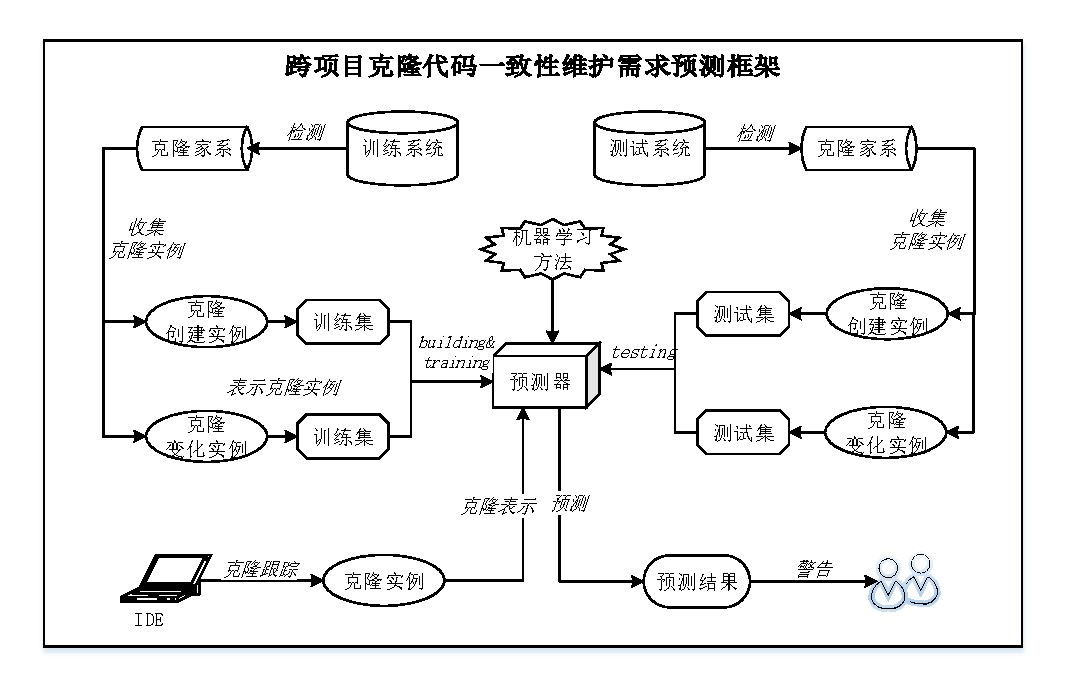
\includegraphics[width = 0.8\textwidth]{framework5.pdf}
\bicaption[framework5]{}{跨项目克隆代码一致性维护需求预测框架}
{Fig.$\!$}{The framework for clone cross-project consistency prediction}
\vspace{-1em}
\end{figure}

为了收集不同系统中的克隆代码创建和变化实例,同样通过构建系统的克隆家系来完成收集工作。使用NiCad来检测软件版本中的所有克隆,并通过在相邻版本的克隆组之间进行映射来构建克隆家系,用于收集克隆实例。然后,通过提取属性值表示克隆创建和变化实例,分别提取代码属性和上下文属性表示克隆创建实例,提取代码属性、上下文属性和历史属性表示克隆变化实例。最后,使用收集到的训练系统的克隆实例训练机器学习模型,并使用其预测测试系统的克隆代码一致性维护需求。

与第三章和第四章相似,每一个克隆实例也有两种不同的预测结果,即满足一致性维护需求和不满足维护需求。
对于满足一致性维护需求实例来说,其在将来的演化中可能会引发一致性变化,程序开发人员需要采取相应的操作。例如,拒绝克隆创建实例或者检查克隆变化实例的一致性。对于不满足一致性维护需求实例来说,其在将来的演化中不会引发一致性变化,程序开发人员不需要需要采取相应的操作,可以放心自由的接受新创建的克隆实例和修改克隆代码。

\BiSection{克隆代码一致性维护需求定义}
{The Definitions for Clone Consistency-Requirement}

在克隆代码的整个演化周期中,克隆片段可能会被开发人员修改,从而导致克隆代码的一致性变化。在本文的第三章和第四章分别提供了两种不同形式的克隆代码一致性变化定义,从而适应于不同时间的克隆一致性维护需求预测中。为了进一步研究跨项目的一致性预测问题,本节统一了第三章和第四章的定义,以应用于跨项目的克隆代码一致性维护需求预测中。因此,克隆代码的一致性变化如下:

\begin{definition}[克隆一致性变化]  
\label{def-change}
给定两个克隆代码片段 $CF_1$和 $CF_2$,且它们被分别地修改为$CF'_1$和$CF'_2$。 如果对于一个非常小的阈值$\tau$,如果克隆代码$CF_1$和$CF_2$的变化满足以下条件,称此变化为一致性变化(Consistent Change) , 
\[
\begin{array}[t]{crl}
 \mathit{textSim}(CF_i, CF'_i) < 1 & \forall i \in \{1,2\} &(1) \\
 \multicolumn{2}{c}{| ~\mathit{textSim}(CF_1,CF'_1)  ~-~ \mathit{textSim}(CF_2,CF'_2) ~| ~< ~ \tau}  & (2)
\end{array}
\]
如果克隆代码变化仅满足条件1,将其称为Type-1一致性变化(Type-1 Consistent Change);如果克隆变化同时满足条件1和条件2,将其称为Type-2一致性变化(Type-2 Consistent Change)。
\end{definition}

定义中克隆代码$ CF_1 $和$ CF_2 $的变化情况由相似性度量$ \mathit {textSim} $进行定义,$textSim$与第三章和第四章计算方式相同。该定义中的两个约束条件共同定义了克隆代码的一致性变化,约束条件$1$确保了克隆代码片段同时被修改,约束条件$2$克隆代码片段发生了一致性的变化,由阈值$\tau$指定。

其中,Type-1一致性变化是克隆创建一致性变化,Type-2一致性变化是克隆变化的一致性变化。这两种不同的一致性变化,将分别应用于两种不同时间的克隆一致性预测中。在克隆代码创建时,目标是避免新创建的克隆代码在其未来演化过程中的一致性变化,及其所导致额外的维护代价。所以,只要两个克隆片段同时变化,即认为会导致额外维护代价。因此,在克隆代码创建时使用使用Type-1一致性变化进行预测。在克隆代码变化时,目的是避免克隆变化可能导致的未来演化中的一致性变化,及其因此所引发的克隆一致性缺陷。所以, 不仅要求两个克隆代码片段同时变化,还需要发生相似的变化,否则将会引入克隆一致性缺陷,因此,在克隆代码变化时使用使用Type-2一致性变化进行预测。

在克隆演化过程中,克隆片段是以克隆组的形式出现在软件系统中。克隆代码的变化情况必然会导致克隆组的变化,而克隆组的变化使用克隆演化模式进行描述,即一致性变化模式。现给出演化过程中克隆组的一致性变化模式定义,如下所示:

\begin{definition}[克隆一致性变化模式] 
\label{def-pattern}
在软件版本 $j+1$中存在一个克隆组$CG'$ ,假设克隆组内至少存在两个克隆代码片段$CF'_1$ 和 $CF'_2$可以与映射到上一版本$j$的克隆组$CG$中,且 $CG$中与之对应的克隆代码片段的 $(CF_1,CF_2)$被修改为$(CF'_1,CF'_2)$。如果克隆片段之间的变化 $(CF_1,CF_2)$变化至$(CF'_1,CF'_2)$满足克隆片段的“Type-1或者Type-2一致性变化”(Type-1 or Type-2 Consistent Change),则称克隆组$CG'$具有Type-1或者Type-2一致性变化模式(Type-1 or  Type-2 Consistent Change Pattern)。
\end{definition}

回顾本章地研究内容是要在两种不同的时刻,跨项目的预测克隆代码的一致性维护需求,结合第三章和第四章的克隆实例的定义,这里将统克隆创建实例和克隆变化实例统一为克隆实例,如下所示:

\begin{definition}[克隆实例] 
\label{def-instance}
将克隆创建实例和克隆变化实例统称为克隆实例。在一个克隆家系$CG$中,克隆家系的根节点为克隆创建实例,并且发生变化的克隆组为克隆变化实例。
\end{definition}

克隆实例在演化过程中可能会发生一致性变化模式,如果不能确保克隆的一致性,将会导致导致额外的维护代价和一致性缺陷。对于克隆创建实例,Type-1一致性变化可能会导致额外的克隆维护代价。对于克隆变化实例,Type-2一致性变化可能会导致克隆一致性缺陷。因此,需要在不同时间预测克隆实例的一致性维护需求,以避免额外的克隆维护代价和一致性缺陷。本章结合第三章和第四章的克隆代码一致性维护需求的定义,将克隆创建和变化的一致性维护需求统一为克隆一致性维护需求定义,如下所示:

\begin{definition}[克隆一致性维护需求] 
 \label{def-requirement}
给定版本 $j$中一个克隆实例,$CG$满足克隆一致性维护需求(Consistency-Requirement),如果在版本$k$中存在一个克隆实例 $CG'$($k>j$)满足以下条件: (1) 在$CG'$中至少存在两个克隆片段在其克隆家系$CGE$中可以映射到克隆实例 $CG$中, (2) $CG'$ 具有“Type-1或者Type-2一致性变化模式”(Type-1 or Type-2 Consistent Change Pattern)。反之,假如克隆实例$CG$ 不满足克隆一致性维护需求条件,称该克隆实例不需要一致性维护(Consistency-Requirement Free,或者Consistency-Free,或者Free)。
\end{definition}

最终,克隆一致性维护需求预测可以转化为以下问题:给定一个克隆实例,克隆创建实例或者克隆变化实例,判断该克隆实例是否满足克隆一致性维护需求。

\BiSection{跨项目一致性维护需求预测数据集}
{The Dataset of Cross-Project Consistency Prediction}

在跨项目的预测中,使用其它系统的数据训练机器学习模型,并预测另外系统的一致性维护需求。因此,需要构建跨项目的数据集,将从训练系统中提取克隆实例作为训练集,从测试系统中提取克隆实例作为测试集。

对于某一个软件系统来讲,通过收集和表示该系统中的克隆实例,可以生成其数据集。因此,生成实验所需的数据集,可以划分为两个部分:收集系统中的克隆实例和表示所收集到的克隆实例

\BiSubsection{跨项目数据收集}
{Collecting Cross-Project Data}

跨项目的数据由软件系统中的克隆实例组成,因此收集系统中的克隆实例,即可以完成收集跨项目的数据。通过构建系统的克隆家系,通过识别其中的克隆演化模式,可以从软件中收集所有的克隆实例。根据定义~\ref{def-instance}~,克隆家系$CGE$中的初始节点即是克隆创建实例,发生变化的克隆组是变化实例。通过构建和遍历克隆家系,可以收集克隆创建和变化实例。

首先,下载系统所有版本的源代码,通过映射所有相邻版本的克隆代码,构建系统中全部克隆家系。然后,通过对比相邻版本的克隆代码,识别克隆家系的克隆演化模式,尤其是克隆一致性变化模式(参考定义~\ref{def-evolutionpattern}~和\ref{def-pattern}~)。根据定义~\ref{def-instance}~通过遍历克隆家系的根节点,可收集系统中所有的克隆创建实例。在收集克隆创建实例后,还需确认该实例中的被复制和被粘贴代码(参见本文第三章收集克隆创建实例小节~\ref{lab-checkcopied}~)。根据定义~\ref{def-instance}通过识别克隆家系中的变化克隆组,便可以收集系统中的克隆变化实例。

根据定义~\ref{def-requirement}~,通过遍历克隆实例所在的克隆家系$CGE$的演化情况,标识克隆实例的一致性维护需求。如果克隆实例在其演化过程中发生了一致性变化模式(定义~\ref{def-pattern}~),则该实例满足一致性维护需求,否则不满足维护需求。

\BiSubsection{克隆实例的属性特征}
{Attributes for Clone Instance}

本文收集到的数据是系统中的克隆实例,因此同样提取相应的属性值表示克隆代码实例。将提取代码、上下文两组属性代表克隆创建实例,提取代码属性、上下文属性和演化属性代表克隆变化实例。其中,代码属性和上下文属性相似,但从不同的角度表示克隆创建实例和变化实例。克隆创建实例中的属性,表示了创建时克隆代码的特征;克隆变化实例中的属性,表示了发生变化的克隆组的特征。

对于克隆创建实例,即被复制和粘贴克隆代码,使用不同的属性进行描述。使用代码属性用于表示被复制的克隆的特征,包括:克隆代码粒度、Halstead属性、结构属性、参数访问数量、总函数调用次数、本地函数调用次数、库函数调用次数、其它调用次数。使用上下文属性用于表示被粘贴的克隆代码的特征,包括:代码相似度、局部克隆标识、文件名相似度、文件名相似度标识、方法名相似度、总参数名相似度、最大参数名相似度、总参数类型相似度、块信息标识。属性具体信息可以参考本文第二章相关属性值部分(第~\ref{lab-creatingattribute}~节克隆创建实例表示)。

对于克隆变化实例,从克隆组的角度重新提取了代码属性和上下文属性,并从演化的角度新增演化属性。代码属性从代码自身的角度,描述了克隆变化实例中克隆代码特征,包括克隆粒度、代码行平均、Halstead属性平均、结构属性平均、总函数调用次数平均、本地函数调用次数平均、库函数调用次数平均、其它调用次数平均。上下文属性描述了克隆变化实例所在克隆组的克隆关系特征,包括代码相似度平均、文件名相似度平均、文件名相似度变量、方法名相似度平均、总参数名相似度平均、最大参数名相似度平均、总参数类型相似度平均、块信息标识。历史属性描述了克隆变化实例所在克隆组在克隆变化发生前的历史演化特征,包括变化实例寿命、历史演化模式统计、当前演化模式、历史变化统计。同时,还提供了克隆变化实例的变化属性。
属性具体信息可以参考本文第二章相关属性值部分(第~\ref{lab-changingattribute}~节克隆变化实例表示)。

数据集生成算法如~\ref{alg-collection}~所示。算法中第1-5行是为克隆代码生成CRD,并使用CRD映射相邻版本的克隆代码,并根据克隆演化模式定义,识别克隆演化模式。第6行是生成系统的克隆家系。第7-10行,分别是收集克隆实例,并标记其一致性维护需求。第11行是初始化数据集。第12-15行是提取相应的属性值表示克隆实例,并且生成数据集。在表示克隆实例时,算法将消耗大量的时间,其时间复杂度为$O(m*n)$,其中m为克隆变化实例的数量。因此,该算法的时间复杂度为$O(m*n)$。

\begin{minipage}{0.8\textwidth}
\centering
\begin{algorithm}[H]
\AlgoBiCaption{数据集生成算法} {The algorithm for generating dataset}
\label{alg-collection}
\KwIn{All source code and code clones from $N$ versions}
\KwOut{The data set of software}
\For{$i$=1 to $N$}
{ 
 Generating CRD to represent each code clone{CFs}\;
 Mapping all the $CFs$ and $CGs$ between the adjacent versions {i} and {i+1}\;
 Identifying all clone evolution pattern in thus two versions according to Definition~\ref{def-evolutionpattern}~and~Definition~\ref{def-pattern}~\;
}
Generating all clone genealogies $CGEs$ with number $N\_cge$\;
\For{$i$=1 to $N\_cge$}
{ 
 Collecting the clone instance that both including clone-creating and changing instances from $CGE\_i$ according to Definition~\ref{def-instance}~\; 
 Labeling all consistency-requirement according to Definition~\ref{def-requirement}~;
}
Initializing all training data set $Creating\_Set$ and $Changing\_Set$for clone creating and changing instances\; 
\For{each clone instance} 
{ 
Generating all attributes for clone creating or changing instance\;
Appending all the attributes to the $Creating\_Set$\ or $Changing\_Set$\;
}
\Return {The data set of software\;}
\end{algorithm}
\end{minipage}

\BiSection{跨项目克隆代码一致性维护需求预测}
{Predicting Clone Cross-Project Consistency-Requirement}

使用收集到的训练系统的克隆实例训练机器学习模型,并预测测试系统的克隆代码的一致性维护需求。从而验证跨项目的克隆一致性需求的预测能力。值得注意的是,将对两种不同的时刻的克隆代码的一致性维护需求分别进行预测(即克隆创建时和克隆变化时),因此会训练两种不同的模型以适用于两个时刻。

对于所测试的软件系统,首先,通过收集训练系统中所有的克隆实例(创建实例和变化实例),并提取相应的属性,用于构建模型训练所需的数据集。然后,调用WEKA中的机器学习算法,分别构建克隆创建和变化的预测器,预测克隆代码的一致性维护需求。

跨项目克隆一致性维护需求预测算法如~\ref{alg-crossperdiction}~所示。算法的第1行为划分训练集和测试集。第2-3行是生成跨项目的数据集。第4行是使用训练集训练机器学习模型。第5行是使用训练的模型在测试集上验证跨项目预测的有效性。

\begin{minipage}{0.8\textwidth}
\centering
\begin{algorithm}[H]
\AlgoBiCaption{跨项目克隆一致性维护需求预测算法} {The algorithm for cross-project predicting clone consistency-requirement}
\label{alg-crossperdiction}
\KwIn{All the projects}
\KwOut{The predictive models}
Dividing the projects into training projects and testing project\;
Generating the $Training\_{Set}$ for training projects\;
Generating the $Testing\_{Set}$ for testing project\;
Calling WEKA to train the models applying training set $Training\_{Set}$\;
Employed this trained model to predict on the $Testing\_{Set}$\;
\Return {The predictive models\;}
\end{algorithm}
\end{minipage}

与第三章和第四章相似,根据定义~\ref{def-requirement}~,克隆实例会有两种不同的状态:需要一致性维护和不需要一致性维护。如下所示:

\begin{itemize}
\item 
需要一致性维护:
若克隆创建实例的预测结果为“需要”,软件开发人员需要谨慎的执行克隆创建操作。因为,该克隆创建实例,在未来演化的过程中可能会引发一致性变化,从而向系统中引入额外的维护代价。若克隆变化实例的预测结果为“需要”,软件开发人员需要检测克隆变化实例所在的克隆组的一致性问题,考虑一致地修改组内其它的克隆代码。因为该克隆变化实例,在未来演化的过程中可能会引发一致性变化,遗忘这种变化会向系统中引入缺陷,从而降低软件质量。
\item
不需要一致性维护:
若克隆创建实例的预测结果为“不需要”,软件开发人员可以自由的执行克隆创建操作,从而节约开发时间提高开发效率。因为该克隆创建实例,在未来演化的过程中不会引发一致性变化,也不会导致额外的维护代价。若克隆创建实例的预测结果为“不需要”,软件开发人员可以自由的修改克隆变化实例所在克隆组的克隆片段。因为,该克隆变化实例,在未来演化的过程中不会引发一致性变化,也不会导致一致性缺陷。
\end{itemize}

在使用已训练好的模型进行预测时,可以与软件开发过程相结合,将该模型嵌入到软件开发环境中,帮助程序开发人员实现边开发边预测克隆实例的一致性维护需求。首先,在软件开发环境中需监测和跟踪克隆代码,识别新产生的克隆实例(克隆创建实例和变化实例)。然后,根据上文描述的代码、上下文和演化属性,提取相应的特征表示相应的克隆实例。最后,使用训练好的预测器预测相应克隆实例的一致性维护需求,根据预测结果提醒程序开发人员采取进一步的操作。

\BiSection{跨项目一致性维护需求预测实验结果与分析}
{Experimental Results and Analysis for Clone Cross-Project Consistency Prediction}

本节给出本章的实验结果与分析,使用五种不同的机器学习方法,对克隆代码创建时和变化时进行跨项目的一致性维护预测。首先简单介绍了实验所使用的实验系统和评估方法,然后详细给出每个实验的结果与分析。

\BiSubsection{实验系统与实验设置}
{Experimental Projects and Methodology}

\BiSubsubsection{实验系统}
{Experimental Projects}

为了解决本章所提出的研究问题,本节选取和第三章和第四章相同的四个开源项目进行实验评估。四个实验系统的基本数据集如表~\ref{instancesta}~所示,分别包括克隆创建实例和克隆变化实例。从该表可以看出,系统中克隆创建实例的数据集的规模要大于克隆变化实例的数据集。克隆创建实例数据集规模为为633到3666个,克隆变化实例的数量范围在159到1040个,系统jEdit是克隆规模最小的系统。同时,表中第3和4列给出了不需要和需要一致性维护的克隆实例的数量和比例。


从表~\ref{instancesta}~中可以观察到两个现象。第一,软件系统中存在大量的克隆创建实例(三个项目中有上千的实例),同时大部分的克隆创建实例在其演化过程中不满足一致性维护要求(比例从59.8\%到88.47\%)。这表明克隆创建操作(即复制和粘贴操作)已经成为开发人员的常用技术,并且它们中的大多数在演化过程中不会在将来引入任何一致的变化,建议开发人员可以使用复制和粘贴操作节省开发时间。第二,在克隆变化实例中,三个系统中只有数百个变化实例,仅有jFreeChart中有1040变化实例。这表明相对于克隆代码在演化过程中不会频繁地发生变化,但也有相当数量的变化。值得注意的,这些变化中需要一致性维护的变化实例比例占相当大的一部分,其比例为33\%到74 \%。克隆代码的一致性变化更容易引发一致性变化,从而导致增加克隆代码一致性缺陷的风险,因此开发人员在软件开发过程中应该更加注意软件开发过程中的克隆变化。

\begin{table}[htbp]
\bicaption[instancesta]{}{实验系统基本数据集信息统计}
{Table$\!$}{The statistics for clone instances in four projects}
\vspace{0.5em}
\centering
\wuhao
\begin{tabular}{ccccc}
\toprule[1.5pt]
~\multirow{2}{*}{类型}&\multirow{2}{*}{系统}&{不需要}&{需要}&\multirow{2}{*}{总数}\\
~&~&{一致性维护}&{一致性维护}&~\\
\midrule[1pt]
\multirow{4}{*}{克隆创建实例}
&ArgoUML&	2574(77.07\%)&	766(22.93\%)&	3340\\
&jEdit&560(88.47\%)&	73(11.53\%)&	633\\
&jFreeChart&	2013(59.80\%)&	1353(40.20\%)&	3366\\
&Tuxguitar&	1016(71.10\%)&	413(28.90\%)&	1429\\
\hline
\multirow{4}{*}{克隆变化实例}
&ArgoUML&288(67.45\%)&139(32.55\%)&427\\
&jEdit&78(49.06\%)&81(50.94\%)&159\\
&jFreeChart&452(43.46\%)&588(56.54\%)&1040\\
&Tuxguitar&91(25.71\%)&263(74.29\%)&354\\
\bottomrule[1.5pt]
\end{tabular}
\end{table}

同时,在跨项目预测是,本文将使用三个系统的数据作为训练集,使用第四个系统作为测试集。因此,给出在进行跨项目预测时训练集规模的大小,如表~\ref{crosssta}~所示。表中使用(To Project)表示被测试的系统为“Project”,并使用除“Project”系统外其它的系统作为训练集。从表中发现克隆创建的训练集规模要远远大于克隆变化的训练集规模,其中克隆创建的训练集规模为5402-8135,克隆变化的训练集规模为940-1821。由于系统之家的差异,不同训练集的规模大小也不相同。

\begin{table}[htbp]
\bicaption[crosssta]{}{跨项目数据集信息统计}
{Table$\!$}{The statistics for cross-project data set}
\vspace{0.5em}
\centering
\wuhao
\begin{tabular}{ccccc}
\toprule[1.5pt]
~\multirow{2}{*}{类型}&\multirow{2}{*}{测试系统}&\multicolumn{3}{c}{训练集规模}\\
\cline{3-5}
~&~&{不需要维护}&{需要维护}&{总数}~\\
\midrule[1pt]
\multirow{4}{*}{克隆创建时}
&(To ArgoUML)&3589(66.12\%)&1839(33.88\%)&5428\\
&(To jEdit)&5603(68.88\%)&2532(31.12\%)&8135\\
&(To jFreeChart)&4150(76.82\%)&1252(23.18\%)&5402\\
&(To Tuxguitar)&	5147(70.13\%)&2192(29.87\%)&	7339\\
\hline
\multirow{4}{*}{克隆变化时}
&(To ArgoUML)&621(39.99\%)&932(60.01\%)&1553\\
&(To jEdit)&831(45.63\%)&990(54.37\%)&1821\\
&(To jFreeChart)&457(48.62\%)&483(51.38\%)&940\\
&(To Tuxguitar)&	818(50.31\%)&808(49.69\%)&1626\\
\bottomrule[1.5pt]
\end{tabular}
\end{table}

\BiSubsubsection{实验设置}
{Experimental Methodology}

为解决跨项目克隆代码一致性预测问题,本章将研究问题划分为三个子研究问题。因此本节也将从三个不同的角度进行实验,并同时回答本文提出的三个子研究问题。三个实验如下,:
\begin{itemize}
\item
跨项目的预测效果实验:将回答第一个子研究问题,使用不同的机器学习模型进行跨项目克隆一致性预测,以验证是否能使用跨项目的数据进行跨项目一致性维护需求预测。
\item
跨项目预测的数据集规模实验:将回答第二个子研究问题,使用不同的数据集训练机器学习模型,并在同一系统上测试跨项目预测模型的预测能力,从而确定训练集规模对跨项目模型预测能力的影响。
\item
跨项目预测的类别选择实验:将回答第三个子研究问题,将探讨在进行跨项目预测时,不同类别克隆实例的一致性预测的效果。实验将使用贝叶斯网络预测不同类别的克隆实例。
\end{itemize}

%%%\BiSubsection{跨项目克隆一致性机器学习方法的实验}
%%%{The Experiments for Five Machine Learning Method for Cross-Project}
\BiSubsection{跨项目克隆一致性维护需求预测效果实验}
{The Effectiveness Experiments for Cross-Project Clone Consistency-Requirement Prediction}

本节将回答本章提出的第一个研究问题:在软件开发初期阶段,在项目自身训练数据不充分的情况下,能否使用其它系统的数据训练模型,并对该系统进行克隆一致性维护需求预测?

在五种机器学习方法上进行了跨项目的预测,并使用同本文第三章和第四章相同的指标评估预测效果,即采用平均精确率(Average Precision)、平均召回率(Average Recall)和平均F值(Average F-measure)进行评价(见本文第~\ref{ref-creatingmetrics}~节和第~\ref{ref-changingmetrics}~节)。

\BiSubsubsection{克隆创建时跨项目预测效果实验结果}
{The Results of Cross-Project Prediction Effectiveness at Creating Time}

对克隆代码创建实例,使用不同的机器学习方法进行跨项目预测,实验结果如~\ref{creatingcrossmethodaverage}~所示。在表中,对于SVM的实验结果使用{*}进行标记表。原因在于:在使用SVM方法进行跨项目预测时,不具备相对应的预测能力,其会将所有的测试数据划分到同一个类别中(规模比较大的类中)。

从表\ref{creatingcrossmethodaverage}~中可以看出,除了SVM方法外,其它的四种机器学习方法,对不同的项目均具有不错的预测效果,并且彼此之间也不存在显著的差异。ArgoUML系统的预测结果较好,其平均F值介于65.3\%-66.7\%之间。对jEdit系统的预测效果最好,为76.2\%-82.6\%,jFreeChart最差,也达到了48.9\%-60.9\%。对于Tuxguitar来说,预测效果也较好,F值为60.3\%-68.3\%。

尽管如此,不同的机器学习方法在不同的跨项目的预测中,其预测能力不是完全一致。对系统ArgoUML和系统Tuxguitar来说,决策树具有最好的预测效果,其F值分别为66.7\%和68.3\%。贝叶斯网络对jEdit系统具有最好的预测效果,F值为82.6\%。而KNN方法对于系统jFreeChart具有最好的预测效果,F值为60.9\%。

因此,针对不同的系统,不推荐程序开发人员选用SVM的方法;但可以使用其它的机器学习方法进行跨项目的一致性维护需求预测;针对不同的软件系统,程序开发人员可以根据预测结果选择最合适的机器学习方法。

\begin{table}[htbp]
\bicaption[creatingcrossmethodaverage]{}{克隆创建时跨项目预测效果}
{Table$\!$}{The effectiveness for cross-project prediction at creating time}
\vspace{0.5em}
\centering
\wuhao
\begin{tabular}{cccccc}
\toprule[1.5pt]
{指标}&{方法}&{To ArgoUML}&{To jEdit}&{To jFreechart}&{To  Tuxguitar}\\
\midrule[1pt]
\multirow{5}{*}{平均Precision}
&BayesNet&	0.638	&0.812	&0.575	&0.648\\
&Natvie&	0.631&	0.783&	0.486&	0.615\\
%&SVM&	0.594&	0.783&	0.358&	0.506\\
&SVM&	0.594*&	0.783*&	0.358*&	0.506*\\
&KNN&	0.629&	0.786&	0.648&	0.581\\
&Tree&	0.629&	0.796&	0.566&	0.704\\
\hline
\multirow{5}{*}{平均Recall}				
&BayesNet&	0.675&	0.844&	0.602&	0.698\\
&Natvie&	0.693&	0.747&	0.54&	0.647\\
%&SVM&	0.771&	0.885&	0.598&	0.711\\
&SVM&	0.771*&	0.885*&	0.598*&	0.711*\\
&KNN&	0.687	&0.741&	0.649&	0.663\\
&Tree&	0.74&	0.844&	0.599&	0.731\\
\hline
\multirow{5}{*}{平均F-Measure}			
&BayesNet&	0.654&	0.826&	0.508&	0.65\\
&Natvie&	0.656&	0.764&	0.489&	0.627\\
%&SVM&	0.671&	0.831&	0.448&	0.591\\
&SVM&	0.671*&	0.831*&	0.448*&	0.591*\\
&KNN&	0.653&	0.762&	0.609&	0.603\\
&Tree&	0.667&	0.818&	0.503&	0.683\\
\bottomrule[1.5pt]
\end{tabular}
\end{table}


%%%对克隆代码创建实例,使用不同的机器学习方法进行跨项目预测,实验结果如~\ref{creatingcrossmethodfree}~和~\ref{creatingcrossmethodmeeting}所示。
%%%
%%%(1)不需要一致性维护实验
%%%
%%%首先,先对不需要一致性维护的克隆实例进行跨项目预测,实验结果如表~\ref{creatingcrossmethodfree}~所示。由表中可以看出,预测效果较好,其中精确率非常好,可以较好的预测克隆代码的一致性维护需求。但是,SVM方法的召回率为1,说明跨项目预测中SVM表现太差,无法预测克隆代码的变化的一致性。在预测结果中,对jEdit的预测效果最好,然
%%%
%%%\begin{table}[htbp]
%%%\bicaption[creatingcrossmethodfree]{}{克隆代码创建时多机器学习跨项目预测}
%%%{Table$\!$}{The effectiveness for cross-project at creating time on free with 5 methods}
%%%\vspace{0.5em}
%%%\centering
%%%\wuhao
%%%\begin{tabular}{cccccc}
%%%\toprule[1.5pt]
%%%{指标}&{方法}&{To ArgoUML}&{To jEdit}&{To jFreechart}&{To  Tuxguitar}\\
%%%\midrule[1pt]
%%%\multirow{5}{*}{Precision}
%%%&BayesNet&	0.766&	0.891&	0.608&	0.73\\
%%%&Natvie&	0.764&	0.876&	0.584&	0.725\\
%%%&SVM&	0.771&	0.885&	0.598&	0.711\\
%%%&KNN&	0.763&	0.878&	0.65&	0.709\\
%%%&Tree&	0.767&	0.885&	0.606&	0.746\\
%%%\hline
%%%\multirow{5}{*}{Recall}				
%%%&BayesNet&	0.831&	0.938&	0.941&	0.908\\
%%%&Natvie&	0.869&	0.832&	0.8	&0.81\\
%%%&SVM&	1&	1&	1&	1\\
%%%&KNN&	0.861&	0.821&	0.896&	0.893\\
%%%&Tree&	0.95&	0.946&	0.94&	0.942\\
%%%\hline
%%%\multirow{5}{*}{F-Measure}					
%%%&BayesNet&	0.797&	0.914&	0.739&	0.81\\
%%%&Natvie&	0.813&	0.853&	0.675&	0.765\\
%%%&SVM&	0.87&	0.939&	0.748&	0.831\\
%%%&KNN&	0.809&	0.849&	0.753&	0.79\\
%%%&Tree&	0.849&	0.915&	0.737&	0.833\\
%%%\bottomrule[1.5pt]
%%%\end{tabular}
%%%\end{table}
%%%
%%%(2)
%%%
%%%\begin{table}[htbp]
%%%\bicaption[creatingcrossmethodmeeting]{}{克隆代码创建时多机器学习跨项目预测}
%%%{Table$\!$}{The effectiveness for cross-project at creating time with 5 methods}
%%%\vspace{0.5em}
%%%\centering
%%%\wuhao
%%%\begin{tabular}{cccccc}
%%%\toprule[1.5pt]
%%%{指标}&{方法}&{To ArgoUML}&{To jEdit}&{To jFreechart}&{To  Tuxguitar}\\
%%%\midrule[1pt]
%%%\multirow{5}{*}{Precision}
%%%&BayesNet&	0.207&	0.205&	0.526	&0.443\\
%%%&Natvie&	0.182&	0.069&	0.34	&0.344\\
%%%&SVM&	0&	0&	0&	0\\
%%%&KNN&	0.178	&0.083&	0.646&	0.268\\
%%%&J48&	0.162	&0.118&	0.506&	0.599\\	
%%%\hline
%%%\multirow{5}{*}{Recall}				
%%%&BayesNet&	0.148&	0.123&	0.098&	0.179\\
%%%&Natvie&	0.098&	0.096&	0.153&	0.245\\
%%%&SVM&	0&	0&	0&	0\\
%%%&KNN&	0.102&	0.123&	0.283&	0.097\\
%%%&Tree&	0.033&	0.055&	0.092&	0.213\\
%%%\hline
%%%\multirow{5}{*}{F-Measure}				
%%%&BayesNet&	0.172&	0.154&	0.165&	0.255\\
%%%&Natvie&	0.127&	0.08&	0.211&	0.286\\
%%%&SVM&	0&	0&	0	&0\\
%%%&KNN&	0.13&	0.099&	0.394&	0.142\\
%%%&Tree&	0.054&	0.075&	0.155&	0.314\\
%%%\bottomrule[1.5pt]
%%%\end{tabular}
%%%\end{table}

\BiSubsubsection{克隆变化时跨项目预测效果实验}
{The Results of Cross-Project Effectiveness Prediction at Changing Time}

对克隆代码变化实例,使用不同的机器学习方法进行跨项目预测,实验结果如~\ref{changingcrossmethodaverage}~所示。在表中,对于SVM的实验结果使用{*}进行标记。原因相同:在使用SVM方法进行跨项目预测时,不具备相对应的预测能力,其会将所有的测试数据划分到同一个类别中(规模比较大的类中)。

从表中可以看出,其它的四种机器学习方法,对不同的项目的预测效果一般,并且彼此之间也不存在显著的差异。分析其预测能力一般的原因,可能是系统中存在的克隆变化实例较少,而项目之间的克隆代码变化也千差万别,所构建的跨项目预测模型并不具有较强的泛化能力。

尽管如此,在克隆变化时进行跨项目预测时,对于不同的系统,存在某一个机器学习方法可以是预测结果的F值达到一个相对最好的预测效果。如(To ArgoUML)中KNN方法的F值为54.6\%,(To jEdit)中Decision Tree的F值为56.7\%,(To jFreeChart)的Native Bayesian方法 为53.3\%。因此,对不同的系统可以选择最合适的机器学习方法进行预测。 

不同的机器学习方法在不同的跨项目的预测中,其预测能力不是完全一致。对系统ArgoUML和系统Tuxguitar来说,KNN具有最好的预测效果,其F值分别为54.6\%和48.7\%。决策树对jEdit系统具有最好的预测效果,F值为56.7\%。而朴素贝叶斯方法对于系统jFreeChart具有最好的预测效果,F值为53.3\%。

结合上一节的贝叶斯网络方法的实验结果,在跨项目的预测中,不推荐程序开发人员选用SVM的方法;但依然可以使用其它的机器学习方法进行跨项目一致性预测,但需要根据项目自身特征,去选择所预测的类别(样本不平衡),即预测数量较多的克隆变化实例类别;在对不同的软件系统进行预测时,程序开发人员可以根据预测结果选择最合适的机器学习方法。

\begin{table}[htbp]
\bicaption[changingcrossmethodaverage]{}{克隆变化时跨项目预测效果}
{Table$\!$}{The effectiveness for cross-project prediction at changing time }
\vspace{0.5em}
\centering
\wuhao
\begin{tabular}{cccccc}
\toprule[1.5pt]
{度量}&{方法}&{To ArgoUML}&{To jEdit}&{To jFreechart}&{To  Tuxguitar}\\
\midrule[1pt]
\multirow{5}{*}{平均Precision}
&BayesNet&	0.591&	0.549&	0.537&	0.602\\
&Natvie&	0.629&	0.547&	0.566&	0.556\\
%&SVM&	0.106&	0.26&	0.611&	0.524\\
&SVM&	0.106*&	0.26*&	0.611*&	0.524*\\
&KNN&	0.624&	0.542&	0.533&	0.623\\
&Tree&	0.629&	0.648&	0.546&	0.638\\
\hline
\multirow{5}{*}{平均Recall}					
&BayesNet&	0.471&	0.547&	0.512&	0.418\\
&Natvie&	0.464&	0.547	&0.538&	0.353\\
%&SVM&	0.326&	0.509&	0.596&	0.322\\
&SVM&	0.326*&	0.509*&	0.596*&	0.322*\\
&KNN&	0.534&	0.541&	0.509&	0.452\\
&Tree&	0.37&	0.604&	0.567&	0.387\\
\hline
\multirow{5}{*}{平均F-Measure}				
&BayesNet&	0.474&	0.546	&0.507&	0.441\\
&Natvie&	0.45&	0.545&	\textbf{0.533}&	0.361\\
%&SVM&	0.16&	0.344&	0.522&	0.32\\
&SVM&	0.16*&	0.344*&	0.522*&	0.32*\\
&KNN&	\textbf{0.546}	&0.54&	0.505&	\textbf{0.478}\\
&Tree&	0.273&	\textbf{0.567}&	0.489&	0.383\\
\bottomrule[1.5pt]
\end{tabular}
\end{table}

%%%%对克隆代码变化实例,使用不同的机器学习方法进行跨项目,实验结果如~\ref{changingcrossmethodfree}~和~\ref{changingcrossmethodmeeting}~所示。
%%%%
%%%%(1)
%%%%
%%%%\begin{table}[htbp]
%%%%\bicaption[changingcrossmethodfree]{}{克隆代码变化时机器学习跨项目预测}
%%%%{Table$\!$}{The effectiveness for cross-project at changing time with 5 methods}
%%%%\vspace{0.5em}
%%%%\centering
%%%%\wuhao
%%%%\begin{tabular}{cccccc}
%%%%\toprule[1.5pt]
%%%%{度量}&{方法}&{To ArgoUML}&{To jEdit}&{To jFreechart}&{To  Tuxguitar}\\
%%%%\midrule[1pt]
%%%%\multirow{5}{*}{Precision}
%%%%&BayesNet&	0.709&	0.535&	0.456&	0.247\\
%%%%&Natvie&	0.761	&0.544&	0.477	&0.228\\
%%%%&SVM&	0&	0	&0.638&	0.219\\
%%%%&KNN&	0.743&	0.529	&0.453	&0.26\\
%%%%&Tree&	0.771	&0.727	&0.508	0.265\\
%%%%\hline
%%%%\multirow{5}{*}{Recall}				
%%%%&BayesNet	&0.365&	0.59&	0.644&	0.615\\
%%%%&Natvie	&0.299&	0.474	&0.677	&0.637\\
%%%%&SVM	&0	&0	&0.164&	0.637\\
%%%%&KNN	&0.472	&0.59&	0.631&	0.615\\
%%%%&Tree	&0.094&	0.308&	0.135	&0.78\\
%%%%\hline
%%%%\multirow{5}{*}{F-Measure}				
%%%%&BayesNet&	0.482	&0.561&	0.534	&0.352\\
%%%%&Natvie	&0.429&	0.507	&0.56	&0.336\\
%%%%&SVM	&0&	0	&0.261&	0.326\\
%%%%&KNN	&0.577&	0.558	&0.527&	0.366\\
%%%%&Tree	&0.167&	0.432	&0.213&	0.396\\
%%%%\bottomrule[1.5pt]
%%%%\end{tabular}
%%%%\end{table}
%%%%
%%%%(2)
%%%%
%%%%\begin{table}[htbp]
%%%%\bicaption[changingcrossmethodmeeting]{}{克隆代码变化时机器学习跨项目预测}
%%%%{Table$\!$}{The effectiveness for cross-project at changing time with 5 methods}
%%%%\vspace{0.5em}
%%%%\centering
%%%%\wuhao
%%%%\begin{tabular}{cccccc}
%%%%\toprule[1.5pt]
%%%%{度量}&{方法}&{To ArgoUML}&{To jEdit}&{To jFreechart}&{To  Tuxguitar}\\
%%%%\midrule[1pt]
%%%%\multirow{5}{*}{Precision}
%%%%&BayesNet&	0.344&	0.562&	0.6&	0.724\\
%%%%&Natvie&	0.357&	0.549&	0.634&	0.67\\
%%%%&SVM	&0.326	&0.509&	0.591	&0.629\\
%%%%&KNN	&0.377&	0.556	&0.594&	0.748\\
%%%%&Tree&	0.334	&0.571&	0.575&	0.767\\
%%%%\hline
%%%%\multirow{5}{*}{Recall}					
%%%%&BayesNet&	0.691&	0.506&	0.41&	0.35\\
%%%%&Natvie	&0.806&	0.617&	0.43&	0.255\\
%%%%&SVM	&1	&1&	0.929&	0.213\\
%%%%&KNN	&0.662&	0.494&	0.415&	0.395\\
%%%%&Tree	&0.942&	0.889	&0.9	&0.251\\
%%%%\hline
%%%%\multirow{5}{*}{F-Measure}				
%%%%&BayesNet&	0.459	&0.532&	0.487	&0.472\\
%%%%&Natvie	&0.494&	0.581&	0.513&	0.369\\
%%%%&SVM&	0.491	&0.675&	0.722&	0.318\\
%%%%&KNN&	0.48&	0.523&	0.488&	0.517\\
%%%%&Tree	&0.493&	0.696&	0.702	&0.378\\
%%%%\bottomrule[1.5pt]
%%%%\end{tabular}
%%%%\end{table}

\BiSubsubsection{讨论}
{Discussion}

综上所述,可以回答第一个研究子问题:

首先,克隆创建时的跨项目预测取得了相对较好的预测效果;在选择合适的机器学习模式前提下,克隆变化时的预测效果也可达到相对不错的预测效果。因此,在软件开发初期,可以使用跨项目的数据进行跨项目的克隆一致性维护需求预测。

然后,在进行跨项目预测时,不建议选择SVM方法进行预测。不同机器学习方法的预测能力不具有显著性差异,可以根据不同的系统选取合适的机器学习方法。


\BiSubsection{跨项目预测训练集规模实验}
{The Experiments of Cross-Project Prediction for Training Size}

在进行克隆代码一致性预测时,训练集的规模会影响到预测的效果。为了探索数据集规模对预测效果的影响,本节实验使用不同的训练集训练模型,并预测克隆代码的一致性。将回答本章提出的第二个研究问题:在进行跨项目的克隆一致性维护需求预测时,训练数据的规模将如何影响跨项目的预测效果?

在五种机器学习方法上进行了跨项目的预测,并使用同本文第三章和第四章相同的指标评估预测效果,即采用平均精确率(Average Precision)、平均召回率(Average Recall)和平均F值(Average F-measure)进行评价(见本文第~\ref{ref-creatingmetrics}~节和第~\ref{ref-changingmetrics}~节)。

首先,进行“一对一”跨项目预测。“一对一”跨项目预测指的是仅使用一个系统的数据作为训练集,另一个系统的数据作为测试集进行跨项目预测。并对目标系统的预测结果进行进行平均,得出“一对一”预测结果(使用“Average”表示)。然后,进行“多对一”跨项目预测。“多对一”跨项目预测指的是,使用三个系统的数据集合称为一个大的训练集,并在另一个系统上进行跨项目预测,得出多对一预测结果(使用“All”表示)。实验结果如表~\ref{creatingcrosssizeaverage}~和表~\ref{changingcrosssizeaverage}~所示。

\BiSubsubsection{克隆创建时跨项目预测数据集规模实验结果}
{The Results of Cross-Project Prediction for Training Size at Creating Time}

在克隆创建时的一对一预测实验中,系统jFreeChart和系统ArgoUML的规模最大,克隆创建实例分别为3366和3340个;系统Tuxguitar规模居中,为1429个;而jEdit具有最小的规模,实例个数仅为159个。在克隆创建时的多对一预测实验中,训练集规模最大的系统为jEdit(8135),其次为系统Tuxguitar(7339),系统ArgoUML和jFreeChart系统的训练集规模最小(分别为5428和5402)。

对克隆创建实例进行跨项目预测,实验结果如表实验结果如表~\ref{creatingcrosssizeaverage}~所示。其中“All”列表示多对一实验结果,“Average”列表示“一对一”实验结果。

通过对比不同系统的跨项目预测结果,可以发现(To jEdit)的实验效果最好,其F值在80\%左右;(To ArgoUML)和(To Tuxguitar)的跨项目预测效果次之,其F值在60-70\%左右;(To jFreeChart)的预测效果最差,F值在50\%左右。根据其训练集的规模大小,可以发现跨项目预测效果和训练集规模存在正相关关系,即训练集的大小影响跨项目的预测能力。因此,在进行跨项目克隆创建预测时,建议扩大其训练集的大小,以达到较好的预测效果。%但是,如何确认训练集规模的大小,仍需进一步的研究确认。

通过对比同一个系统的“Average”和“All”列,在4个系统中全部的F值中,“All”列具有较好的预测效果(表中大多数“All”列的数值要大于“Average”列)。但是,通过比较“Average”和“All”列中数据,发现两列的数据相差不大。因此,在对于某一个具体的测试系统,在跨项目预测中,对于同一个测试系统而言,由于项目之间的差异,训练集规模的大小并不能起到决定性作用。因此,可以考虑在保证一定规模训练数据的基础上,对训练数据进行进一步的过滤,缩小项目之间的差异,从而提升跨项目的预测效果。但是,如何过滤和优选跨项目预测的训练数据,从而缩小项目之间的差异,仍需进一步的研究确认。

\begin{table} [htbp]
\bicaption[creatingcrosssizeaverage]{}{创建时跨项目预测数据集规模实验}
{Table$\!$}{The effectiveness of cross-project for training size at creating time}
\vspace{0.5em}
\centering
\footnotesize
\begin{tabular}{cccccccccc}
\toprule[1.5pt]
~\multirow{2}{*}{指标}&\multirow{2}{*}{方法}&\multicolumn{2}{c}{To ArgoUML}&\multicolumn{2}{c}{To jEdit}&\multicolumn{2}{c}{To jFreeChart}&\multicolumn{2}{c}{To  Tuxguitar}\\
\cline{3-10}
~&~&{Average}&{All}&{Average}&{All}&{Average}&{All}&{Average}&{All}\\
\midrule[1pt]
\multirow{5}{*}{平均Precision}
&BayesNet&0.633&0.638&0.810&	0.812&0.556&0.575&0.633&0.648\\
&Natvie&0.629&0.631&0.792&0.783&0.502&0.486&	0.606&0.615\\
&SVM&0.657&0.594&0.783&0.783&	0.358&0.358&0.506&	0.506\\
&KNN&0.629&0.629&0.815&0.786&	0.617&0.648&0.587&	0.581\\
&Tree&0.686&	0.629&0.782&0.796&	0.530&0.566&0.594&0.704\\
\hline
\multirow{5}{*}{平均Recall}															
&BayesNet&0.670&0.675&	0.752&0.844&	0.606&0.602&	0.674&0.698\\
&Natvie&0.669&0.693&	0.754&0.747&	0.564&0.54&0.643&0.647\\
&SVM&	0.809&0.771&0.885&	0.885&0.598&0.598&0.711&0.711\\
&KNN&	0.681&0.687&0.762&0.741&0.635&0.649&0.655&	0.663\\
&Tree	&0.764&	0.74&	0.803&0.844&0.595&	0.599&0.688&0.731\\
\hline
\multirow{5}{*}{平均F-Measure}					
&BayesNet&0.645&0.654&	0.768&0.826&0.516&0.508&0.631&0.65\\
&Natvie&0.645&0.656&	0.774&0.764	&0.488&	0.489	&0.617&0.627\\
&SVM&	0.724&0.671&0.831&	0.831&0.448&0.448&	0.591&0.591\\
&KNN&	0.651&0.653&0.781&	0.762&0.579	&0.609&	0.601	&0.603\\
&Tree	&0.703&	0.667&0.789&0.818&	0.484	&0.503&	0.612	&0.683\\
\bottomrule[1.5pt]
\end{tabular}
\end{table}


%%%%%%\begin{sidewaystable} [htbp]
%%%%%%\bicaption[creatingcrosssizefree]{}{创建时跨项目预测数据集选择实验(free)}
%%%%%%{Table$\!$}{The effectiveness of cross-project for training size selection at creating time(free)}
%%%%%%\vspace{0.5em}
%%%%%%\centering
%%%%%%\wuhao
%%%%%%\begin{tabular}{cccccccccc}
%%%%%%\toprule[1.5pt]
%%%%%%~\multirow{2}{*}{度量}&\multirow{2}{*}{方法}&\multicolumn{2}{c}{To ArgoUML}&\multicolumn{2}{c}{To jEdit}&\multicolumn{2}{c}{To jFreeChart}&\multicolumn{2}{c}{To  Tuxguitar}\\
%%%%%%\cline{3-10}
%%%%%%~&~&{Average}&{All}&{Average}&{All}&{Average}&{All}&{Average}&{All}\\
%%%%%%\midrule[1pt]
%%%%%%\multirow{5}{*}{Precision}
%%%%%%&BayesNet&	0.763&	0.766&	0.887&	0.891&	0.615&	0.608&0.729&	0.731\\
%%%%%%&Natvie&	0.760&	0.764&	0.880&	0.876&	0.593&	0.584&	0.720	&0.725\\
%%%%%%&SVM&	0.809&	0.771	&0.885&	0.885&	0.598&	0.598&	0.711&	0.711\\
%%%%%%&KNN&	0.762&	0.763	&0.894&	0.878&	0.641&	0.65&	0.709&	0.709\\
%%%%%%&Tree	&0.785	&0.767&0.882	&0.885&	0.620	&0.606&	0.718&	0.746\\
%%%%%%\hline
%%%%%%\multirow{5}{*}{Recall}								
%%%%%%&BayesNet&	0.829	&0.831	&0.824	&0.938	&0.929	&0.941&	0.866&	0.908\\
%%%%%%&Natvie&	0.831	&0.869	&0.834	&0.832	&0.862	&0.8&	0.815&	0.81\\
%%%%%%&SVM&	1&	1&	1&	1&	1&	1	&1	&1\\
%%%%%%&KNN&	0.853&	0.861&	0.828&	0.821&	0.899&	0.896&	0.873&	0.893\\
%%%%%%&Tree	&0.958&	0.95&	0.904	&0.946	&0.954&	0.94&	0.935&	0.942\\
%%%%%%\hline
%%%%%%\multirow{5}{*}{F-Measure}							
%%%%%%&BayesNet&	0.792&	0.797&	0.848&	0.914&	0.739&	0.739&	0.789&0.81\\
%%%%%%&Natvie&	0.793&	0.813	&0.852	&0.853	&0.702	&0.675	&0.764	&0.765\\
%%%%%%&SVM&	0.893	&0.87	&0.939	&0.939	&0.748	&0.748	&0.831&	0.831\\
%%%%%%&KNN&	0.804	v0.809&	0.857	&0.849	&0.747	&0.753	&0.781&	0.79\\
%%%%%%&Tree&	0.863	&0.849&	0.889&	0.915&	0.739&	0.737	&0.810	&0.833\\
%%%%%%\bottomrule[1.5pt]
%%%%%%\end{tabular}
%%%%%%\end{sidewaystable}
%%%%%%
%%%%%%\begin{sidewaystable} [htbp]
%%%%%%\bicaption[creatingcrosssizemeeting]{}{创建时跨项目预测数据集选择实验(meeting)}
%%%%%%{Table$\!$}{The effectiveness of cross-project for training size selection at creating time(meeting)}
%%%%%%\vspace{0.5em}
%%%%%%\centering
%%%%%%\wuhao
%%%%%%\begin{tabular}{cccccccccc}
%%%%%%\toprule[1.5pt]
%%%%%%~\multirow{2}{*}{度量}&\multirow{2}{*}{方法}&\multicolumn{2}{c}{To ArgoUML}&\multicolumn{2}{c}{To jEdit}&\multicolumn{2}{c}{To jFreeChart}&\multicolumn{2}{c}{To  Tuxguitar}\\
%%%%%%\cline{3-10}
%%%%%%~&~&{Average}&{All}&{Average}&{All}&{Average}&{All}&{Average}&{All}\\
%%%%%%\midrule[1pt]
%%%%%%\multirow{5}{*}{Precision}
%%%%%%&BayesNet&	0.198&	0.207&	0.214&	0.205&	0.469&	0.526&0.399&	0.443\\
%%%%%%&Natvie&	0.186&	0.182&	0.113&	0.069&	0.367&	0.34&	0.325	&0.344\\
%%%%%%&SVM&	0&	0&	0&0&	0&	0&0&	0\\
%%%%%%&KNN&	0.181&	0.178&	0.208&	0.083&	0.581&	0.646&	0.286&	0.268\\
%%%%%%&Tree	&0.357&	0.162&	0.067&	0.118&	0.422&	0.506&	0.297&	0.599\\
%%%%%%\hline
%%%%%%\multirow{5}{*}{Recall}								
%%%%%%&BayesNet&0.136&	0.148&	0.205&	0.123&	0.127&	0.098&	0.203&	0.179\\
%%%%%%&Natvie&	0.123&	0.098&	0.141&	0.096&	0.119&	0.153&	0.219&	0.245\\
%%%%%%&SVM&	0&	0&	0&	0&	0&	0&	0	&0\\
%%%%%%&KNN&	0.105&	0.102&	0.251&	0.123&	0.243&	0.283&	0.120&	0.097\\
%%%%%%&Tree	&0.112	&0.033&	0.023&	0.055&	0.062	&0.092&	0.081	&0.213\\
%%%%%%\hline
%%%%%%\multirow{5}{*}{F-Measure}									
%%%%%%&BayesNet&0.151&	0.172&	0.159&	0.154&	0.184&	0.165&	0.244&	0.255\\
%%%%%%&Natvie&	0.145&	0.127&	0.110&	0.08&	0.176&	0.211&	0.257&	0.286\\
%%%%%%&SVM&	0&	0&	0&	0&	0&	0&	0&	0\\
%%%%%%&KNN&	0.132&	0.13&	0.201&	0.099&	0.328&	0.394&	0.158&	0.142\\
%%%%%%&Tree&	0.167&	0.054&	0.027&	0.075&	0.105&	0.155&	0.126&	0.314\\
%%%%%%\bottomrule[1.5pt]
%%%%%%\end{tabular}
%%%%%%\end{sidewaystable}

\BiSubsubsection{克隆变化时跨项目预测数据集规模实验结果}
{The Results of Cross-ProjectPrediction for Training Size at Changing Time}

对克隆变化实例进行预测,实验结果如表实验结果表~\ref{changingcrosssizeaverage}~所示。

根据数据集规模的统计分析(表~\ref{instancesta}~和表\ref{crosssta}~),克隆创建实例的数量要远多于克隆变化实例的数量,即创建实例具有上千的规模(633-3366个),变化实例仅有数百的规模(159-1040)。结合对两种实例的跨项目预测结果,发现前者的跨项目预测效果要优于后者。因此,尽管在不同的时刻进行预测,练数据的规模同样会影响到跨项目的预测效果。建议在可能的情况下,增加训练集的数据。

在克隆变化时的一对一预测实验中,系统jFreeChart规模最大,克隆变化实例为1040个;系统ArgoUML和系统Tuxguitar的规模居中,分别为427和3549个;而jEdit具有最小的规模,实例个数仅为159个。在克隆变化时的多对一预测实验中,训练集规模最大的系统为jEdit(1821),其次为系统ArgoUML(1553)和系统Tuxguitar(1626),系统jFreeChart的训练集规模最小,为940。

通过对比不同系统的跨项目预测结果,可以发现(To jEdit)的实验效果最好,其F值除SVM外介于54\%-56.7\%之间;(To jFreeChart)的预测效果次之,F值在48.9\%-53.3\%之间;而(To ArgoUML)和(To Tuxguitar)预测效果最差,大部分的F值低于50\%。根据其训练集的规模大小,可以发现跨项目预测效果和训练集规模也存在一定的正相关关系。但是,其相关性不如克隆创建实例。究其原因可能是因为:克隆变化实的训练集规模仅仅在几百之间,和创建实例的数量相差较大。克隆变化时跨项目预测的数据集规模较小,导致模型无法较好的训连。%但是,如何确认训练集具体规模的大小,仍需进一步的研究确认。

通过对比每个项目的“Average”和“All”列,在4个系统中全部的F值中,“All”列具有较好的预测效果。具体地,对系统(To jEdit)和(To jFreeChart),“All”列的预测效果均优于“Average”列。但是,通过比较“Average”和“All”列中数据,发现两列的数据相差不大。因此,在对于某一个具体的测试系统,在跨项目预测中,由于项目之间的差异,训练集的大小并不能起到决定性作用。因此,可以考虑在保证一定规模训练数据的基础上,对训练数据进行进一步的过滤,缩小项目之间的差异,从而提升跨项目的预测效果。但是,如何过滤和优选跨项目预测的训练数据,从而缩小项目之间的差异,仍需进一步的研究确认。

\begin{table} [htbp]
\bicaption[changingcrosssizeaverage]{}{克隆变化的跨项目预测数据集规模实验}
{Table$\!$}{The effectiveness of cross-project for training size at changing time}
\vspace{0.5em}
\centering
\footnotesize
\begin{tabular}{cccccccccc}
\toprule[1.5pt]
~\multirow{2}{*}{指标}&\multirow{2}{*}{方法}&\multicolumn{2}{c}{To ArgoUML}&\multicolumn{2}{c}{To jEdit}&\multicolumn{2}{c}{To jFreeChart}&\multicolumn{2}{c}{To  Tuxguitar}\\
\cline{3-10}
~&~&{Average}&{All}&{Average}&{All}&{Average}&{All}&{Average}&{All}\\
\midrule[1pt]
\multirow{5}{*}{平均Precision}
&BayesNet&	0.595&	0.591&0.480&	0.549&	0.552&	0.537&	0.575&	0.602\\
&Natvie&	0.596&	0.629	&0.541&	0.547&	0.548&	0.566&	0.548&	0.556\\
&SVM&	0.106&	0.106&	0.254&	0.26&	0.276	&0.611&	0.390&	0.524\\
&KNN&	0.605&	0.624&	0.517&	0.542&	0.515&	0.533&	0.617&	0.623\\
&Tree	&0.616&	0.629&	0.490&	0.648&	0.485	&0.546	&0.616	&0.638\\
\hline
\multirow{5}{*}{平均Recall}								
&BayesNet&	0.513&	0.471&	0.482&	0.547&	0.522	&0.512&	0.389	&0.418\\
&Natvie&	0.496&	0.464&	0.541	&0.547&0.531	&0.538&0.398	&0.353\\
&SVM&	0.343&	0.326&	0.491&	0.509&	0.503&	0.596&	0.581&	0.322\\
&KNN&	0.533&	0.534&	0.512	&0.541&	0.498&	0.509&	0.449&	0.452\\
&Tree	&0.387&	0.37&	0.501	&0.604&	0.516&	0.567&	0.550&	0.387\\
\hline
\multirow{5}{*}{平均F-Measure}								
&BayesNet&	0.491	&0.474&	0.456&	0.546	&0.501&	0.507&	0.383	&0.441\\
&Natvie&	0.481&	0.45&	0.533&	0.545&	0.526&	0.533&	0.407&	0.361\\
&SVM&	0.160	&0.16	&0.337	&0.344	&0.360	&0.522	&0.457	&0.32\\
&KNN&	0.453&	0.546	&0.446&	0.54&	0.459	&0.505	&0.474&	0.478\\
&Tree&	0.296	&0.273	&0.441&	0.567	&0.407&	0.489	&0.500&	0.383\\
\bottomrule[1.5pt]
\end{tabular}
\end{table}

%%%%\begin{sidewaystable} [htbp]
%%%%\bicaption[changingcrosssizefree]{}{变化时跨项目预测数据集选择实验(free)}
%%%%{Table$\!$}{The effectiveness of cross-project for training size selection at changing time(free)}
%%%%\vspace{0.5em}
%%%%\centering
%%%%\wuhao
%%%%\begin{tabular}{cccccccccc}
%%%%\toprule[1.5pt]
%%%%~\multirow{2}{*}{指标}&\multirow{2}{*}{方法}&\multicolumn{2}{c}{To ArgoUML}&\multicolumn{2}{c}{To jEdit}&\multicolumn{2}{c}{To jFreeChart}&\multicolumn{2}{c}{To  Tuxguitar}\\
%%%%\cline{3-10}
%%%%~&~&{Average}&{All}&{Average}&{All}&{Average}&{All}&{Average}&{All}\\
%%%%\midrule[1pt]
%%%%\multirow{5}{*}{Precision}
%%%%&BayesNet&	0.706	&0.709&	0.455&	0.535&	0.462&	0.456&	0.241&	0.247\\
%%%%&Natvie&	0.711	&0.761	&0.529	&0.544&	0.464	&0.477	&0.221	&0.228\\
%%%%&SVM&	0	0&	0.164&	0	&0.145&	0.638&	0.086&	0.219\\
%%%%&KNN&	0.712&	0.743&	0.502&	0.529&	0.421&	0.453&	0.257&	0.26\\
%%%%&Tree&	0.750&	0.771&	0.465&	0.727&	0.417&	0.508&	0.317&	0.265\\
%%%%\hline
%%%%\multirow{5}{*}{Recall}								
%%%%&BayesNet&	0.476&	0.365&	0.500&	0.59&	0.624&	0.644&	0.634&	0.615\\
%%%%&Natvie&	0.421&	0.299&	0.462&	0.474&	0.580&	0.677&	0.531&	0.637\\
%%%%&SVM	&0&	0	&0.333&	0&	0.333&	0.164&	0.333&	0.637\\
%%%%&KNN	&0.509&	0.472	&0.496	&0.59&	0.526	&0.631	&0.600&	0.615\\
%%%%&Tree	&0.127&	0.094&	0.368&	0.308&	0.357&	0.135&	0.425&	0.78\\
%%%%\hline
%%%%\multirow{5}{*}{F-Measure}							
%%%%&BayesNet&	0.521&	0.482&	0.455&	0.561&	0.515&	0.534&	0.343&	0.352\\
%%%%&Natvie&	0.495&	0.429&	0.487&	0.507&	0.511&	0.56&	0.307&	0.336\\
%%%%&SVM&	0&	0&	0.219&	0&	0.202&	0.261&	0.136&	0.326\\
%%%%&KNN&	0.567&	0.577&	0.473&	0.558&	0.451&	0.527&	0.359&	0.366\\
%%%%&Tree&	0.199&	0.167&	0.355&	0.432&	0.279&	0.213&	0.288&	0.396	\\							
%%%%\bottomrule[1.5pt]
%%%%\end{tabular}
%%%%\end{sidewaystable}
%%%%
%%%%\begin{sidewaystable} [htbp]
%%%%\bicaption[changingcrosssizemeeting]{}{变化时跨项目预测数据集选择实验(meeting)}
%%%%{Table$\!$}{The effectiveness of cross-project for training size selection at changing time(meeting)}
%%%%\vspace{0.5em}
%%%%\centering
%%%%\wuhao
%%%%\begin{tabular}{cccccccccc}
%%%%\toprule[1.5pt]
%%%%~\multirow{2}{*}{指标}&\multirow{2}{*}{方法}&\multicolumn{2}{c}{To ArgoUML}&\multicolumn{2}{c}{To jEdit}&\multicolumn{2}{c}{To jFreeChart}&\multicolumn{2}{c}{To  Tuxguitar}\\
%%%%\cline{3-10}
%%%%~&~&{Average}&{All}&{Average}&{All}&{Average}&{All}&{Average}&{All}\\
%%%%\midrule[1pt]
%%%%\multirow{5}{*}{Precision}
%%%%&BayesNet&	0.365&	0.344&	0.505&	0.562&	0.620&	0.6	&0.69&	0.724\\
%%%%&Natvie&	0.358	&0.357	&0.552	&0.549	&0.613	&0.634	&0.662	&0.67\\
%%%%&SVM&	0.326	&0.326&	0.339&	0.509&	0.377&	0.591&	0.495&	0.629\\
%%%%&KNN&	0.381&	0.377	&0.531&	0.556&	0.588&	0.594&	0.742&	0.748\\
%%%%&Tree&	0.340&	0.334	&0.514&	0.571&	0.538&	0.575&	0.719&	0.767\\
%%%%\hline
%%%%\multirow{5}{*}{Recall}										
%%%%&BayesNet&	0.590&	0.691&	0.465&	0.506&	0.442&	0.41&	0.304&	0.35\\
%%%%&Natvie&	0.650&	0.806&	0.617&	0.617&	0.492&	0.43&	0.352&	0.255\\
%%%%&SVM&	1&	1&	0.667&	1&	0.667&	0.929&	0.667&	0.213\\
%%%%&KNN&	0.583	&0.662	&0.527	&0.494	&0.476	&0.415&	0.397&	0.395\\
%%%%&Tree	&0.923&	0.942&	0.630&	0.889&	0.638&	0.9&	0.593&	0.251\\
%%%%\hline
%%%%\multirow{5}{*}{F-Measure}									
%%%%&BayesNet&	0.430&0.459&	0.457&	0.532&	0.490&	0.487&	0.397&	0.472\\
%%%%&Natvie&	0.452&	0.494&	0.578&	0.581&	0.538&	0.513&	0.442&	0.369\\
%%%%&SVM&	0.491&	0.491&	0.450&	0.675&	0.481&	0.722&	0.569&	0.318\\
%%%%&KNN&	0.445&	0.48&	0.506&	0.523&	0.498&	0.488&	0.513&	0.517\\
%%%%&Tree&	0.496&	0.493&	0.524&	0.696&	0.505&	0.702&	0.573&	0.378\\
%%%%\bottomrule[1.5pt]
%%%%\end{tabular}
%%%%\end{sidewaystable}

\BiSubsubsection{讨论}
{Discussion}

综上所述,可以回答第二个研究子问题:

首先,在跨项目预测中,训练集的大小会影响到预测的效果,较大的训练集可以达到较强的预测能力。但是,如何确定训练集大小仍需进一步的研究确定。

其次,但针对某特定的系统来讲,训练集的大小并不能起到决定性的作用,原因可能在于项目自身的差距较大。因此,如何对训练集项目的数据进行优选和过滤,可能会提高跨项目的预测能力,但是如何进行优选跨项目预测的训练数据,从而降低训练系统和测试系统之间的差异,仍需进一步的研究确定。

\BiSubsection{跨项目预测的类别选择实验}
{The Experiment of Cross-Project Prediction for Category Selection}

在贝叶斯网络的实验中,本节将回答本章提出的第三个研究问题:在进行跨项目的克隆一致性维护需求预测时,应该预测哪一类别的克隆代码实例,是否对两种实例都具有一致的预测效果?

相似地,使用三个项目的克隆实例训练贝叶斯网络,并在第四个实验系统上进行一致性预测。采用和第三章和第四章相同的评价指标,评估跨项目预测的能力。对需要一致性维护的克隆实例,使用警告率(Warning Rate)、精确率(Precision Rate)和召回率(Recall Rate)进行评估;对不需要一致性维护的克隆实例,使用推荐率(Recommendation Rate )、精确率(Precision Rate)和召回率(Recall Rate)进行评估,详见本文第~\ref{ref-creatingmetrics}~节和第~\ref{ref-changingmetrics}~节。实验也在两个时刻进行了预测,即克隆代码创建时和克隆代码变化时。

\BiSubsubsection{克隆创建时跨项目预测的类别选择实验结果}
{The Results of Cross-Project Prediction for Category Selection at Creating Time}

本节在克隆代码创建时,四个系统上的实验结果如表~\ref{copycrossfreebaysian}~和~\ref{copycrossmeetingbaysian}所示。

(1)不需要一致性维护

对于克隆创建实例,由统计结果可以看出(~表\ref{instancesta}~),系统中大部分的实例都是不需要进行一致性维护的克隆实例,其比例为59.80-88.47\%。对其进行跨项目一致性预测,其预测结果如表~\ref{copycrossfreebaysian}~所示。

从表中可以看出,四个系统的精确率和召回率依然达到了较高的水平,其中精确率在60.01\%--91.20\%之间,召回率56.06\%--91.43\%之间。同时,通过对比发现jEdit的预测效果最好(精确率较高),而jFreeChart预测效果最差。分析原因可能是由于jEdit系统的训练集最大,模型训练最充分,而jFreeChart则与之相反。

将实验结果与第三章的全属性实验进行对比(表~\ref{copyallfree}~),可以发现四个系统的预测效果都有了不同程度的下降,但是目跨项目的预测效果依然是可以接受的。

因此,预测模型的预测能力会依赖于自身系统数据,建议优先选用系统自身的数据进行一致性为需求预测;在软件开发初期,自身系统训练数据较少,而不足以较好的训练模型的情况下,可以使用其它系统的数据对模型进行跨项目预测。

\begin{table}[htbp]
\bicaption[copycrossfreebaysian]{}{克隆创建的贝叶斯网络跨项目预测实验结果(不需维护)}
{Table$\!$}{The effectiveness for cross-project with Bayesian network at creating time(free)}
\vspace{0.5em}
\centering
\wuhao
\begin{tabular}{ccccc}
\toprule[1.5pt]
{测试系统}&{阈值}&{推荐率(\%)}&{精确率(\%)}&{召回率(\%)}\\
\midrule[1pt]
\multirow{5}{*}{ArgoUML}
&0.01&	59.16&	73.03&	56.06\\
&0.05&	67.57&	75.59&	66.28\\
&0.10&	71.95&	76.28&	71.21\\
&0.15&	74.10&	76.40&	73.47\\
&0.20&	75.81&	76.18&	74.94\\
\hline
\multirow{5}{*}{jEdit}
&0.01&	78.99&	91.20&	81.43\\
&0.05&	85.62&	90.41&	87.50\\
&0.10&	87.52&	90.25&	89.29\\
&0.15&	89.10&	89.72&	90.36\\
&0.20&	90.21&	89.67&	91.43\\
\hline
\multirow{5}{*}{jFreeChart}
&0.01&	74.48&	60.07&	74.81\\
&0.05&	82.92&	60.01&	83.21\\
&0.10&	86.51&	60.65&	87.73\\
&0.15&	88.38&	61.01&	90.16\\
&0.20&	88.92&	60.84&	90.46\\
\hline
\multirow{5}{*}{Tuxguitar}
&0.01&	59.55&	75.44&	63.19\\
&0.05&	70.40&	74.16&	73.43\\
&0.10&	74.74&	74.91&	78.74\\
&0.15&	78.38&	74.29&	81.89\\
&0.20&	80.76&	74.00&	84.06\\
\bottomrule[1.5pt]
\end{tabular}
\end{table}

(2)需要一致性维护

对于克隆创建实例,由统计结果可以看出(~表\ref{instancesta}~),系统中仅有少量的实例满足一致性维护需求,其比例为11.53-40.20\%。对其进行跨项目一致性预测,实验结果如~\ref{copycrossmeetingbaysian}所示。

从表中可以看出,四个系统的预测效果都比较差,精确率在15.36\%--61.01\%之间,召回率则更低,仅在10\%徘徊。分析原因是克隆创建实例的样本不平衡,其中大部分的数据是不需要一致性维护。所以,所训练的模型不够完善,跨项目预测能力无法达到实际应用的水平。

与第三章全属性实验进行对比(表~\ref{copyallmeeting}~),发现四个系统的跨项目预测效果下降的均十分严重。因此,对需要一致性维护的克隆创建实例,不建议使用跨项目的方式进行克隆一致性预测。

因此, 对于需要一致性维护的克隆创建实例,本文同样不建议使用跨项目的方式对需要一致性维护的克隆创建实例进行预测,而是选择自身数据进行预测。在开发初期由于缺乏数据问题,建议程序开发人员选择对不需要的克隆实例进行预测。

\begin{table}[htbp]
\bicaption[copycrossmeetingbaysian]{}{克隆创建的贝叶斯网络方法跨项目预测实验结果(需要维护)}
{Table$\!$}{The effectiveness for cross-project with Bayesian network at creating time(meeting)}
\vspace{0.5em}
\centering
\wuhao
\begin{tabular}{ccccc}
\toprule[1.5pt]
{测试系统}&{阈值}&{警告率(\%)}&{精确率(\%)}&{召回率(\%)}\\
\midrule[1pt]
\multirow{5}{*}{ArgoUML}
&0.90&	8.38&	15.36&	5.61\\
&0.80&	10.30&	15.70&	7.05\\
&0.70&	12.75&	20.19&	11.23\\
&0.60&	14.52&	18.76&	11.88\\
&0.50&	16.38&	20.66&	14.75\\
\hline
\multirow{5}{*}{jEdit}
&0.90&	2.37&	33.33&	6.85\\
&0.80&	3.95&	24.00&	8.22\\
&0.70&	5.53&	20.00&	9.59\\
&0.60&	6.64&	19.05&	10.96\\
&0.50&	6.95&	20.45&	12.33\\
\hline
\multirow{5}{*}{jFreeChart}
&0.90&	2.70&	50.55&	3.40\\
&0.80&	4.72&	61.01&	7.17\\
&0.70&	6.36&	54.67&	8.65\\
&0.60&	6.95&	53.42&	9.24\\
&0.50&	7.46&	52.59&	9.76\\
\hline
\multirow{5}{*}{Tuxguitar}
&0.90&	6.02&	53.49&	11.14\\
&0.80&	7.98&	55.26&	15.25\\
&0.70&	8.89&	52.76&	16.22\\
&0.60&	10.15&	49.66&	17.43\\
&0.50&	11.69&	44.31&	17.92\\
\bottomrule[1.5pt]
\end{tabular}
\end{table}

(3)小结

在克隆创建的跨项目的预测中,所构建的预测模型的有效性会依赖于系统自身的某些特征。因此,本文建议优先选用自身的数据进行模型训练,并对自身系统进行预测。

当自身系统的数据太少而不足以训练模型时,由于系统具有较多的不需要一致性维护的克隆创建实例,而需要实例较少。所训练的跨项目预测模型可以较好的预测不需要一致性维护的克隆实例,而对需要维护的预测效果较差。因此,对需要一致性维护的克隆创建实例,本文不建使用系统交叉的方式进行一致性维护进行预测。

在软件开发初期,可以使用跨项目预测的方式,对克隆创建实例进行不需要一致性维护需求预测,仅仅允许此类的克隆实例产生,从而避免一致性维护代价。

\BiSubsubsection{克隆变化时跨项目预测的类别选择实验结果}
{The Results of Cross-Project Prediction for Category Selection at Changing Time}

本节给出在克隆代码变化时,四个系统上的实验结果如表~\ref{changecrossfreebaysian}~和~\ref{changecrossmeetingbaysian}所示。

(1)不需要一致性维护

对于克隆变化实例,根据统计结果(~表\ref{instancesta}~),在系统ArgoUML中,不需要维护的变化实例较多(比例为67.45\%),其它三个系统中不需要一致性维护的实例较少(比例为25.71-49.06\%)。其中,系统Tuxguitar具有最少的需要维护的实例,比例为25.71\%,剩余两个系统中需要和不需要维护的实例数量相差不大。

对不需要一致性维护的克隆变化实例,跨项目一致性预测结果如表~\ref{changecrossfreebaysian}~所示。从表中可以看出,ArgoUML的精确率最好,达71.72\%以上,系统jEdit和jFreeChart的预测效果在50\%左右,而Tuxguitar的预测效果最差。结合数据的不平衡性,发现预测效果向需要一致性维护的实例偏移。因此,精确度预测效果与样本自身的特征有关联关系,即最好选择向数据较多的一侧进行预测。同时,四个系统的召回率都不尽如意,未能达到较好的预测效果。分析原因,是由于样本之间具有较大的差异,跨项目数据无法较好的拟合被测试系统的样本数据。

结合全属性实验的实验结果(表~\ref{changeallfree}~),可以发现当使用自身系统的数据作为训练集且训练集足够大时,预测模型有效的。因此,本文建议使用系统自身的数据进行一致性预测,不建议使用跨项目的形式进行预测。

然而,在软件开发的初期阶段,由于缺乏足够数量的克隆变化实例,不能很好的训练模型时,开发人员可以使用本文第三章提出的方法在克隆创建时预测克隆代码的一致性,从而仅允许那些不需要一致性维护的克隆实例产生。在软件演化到了足够的版本时,随着来自其自己的克隆变化数据的增加,开发人员可以使用自身数据重新训练模型以预测项目中克隆变化的一致性。

\begin{table}[htbp]
\bicaption[changecrossfreebaysian]{}{克隆变化的贝叶斯网络方法跨项目预测实验结果(不需维护)}
{Table$\!$}{The effectiveness for cross-project with Bayesian network at changing time(free)}
\vspace{0.5em}
\centering
\wuhao
\begin{tabular}{ccccc}
\toprule[1.5pt]
{测试系统}&{阈值}&{推荐率(\%)}&{精确率(\%)}&{召回率(\%)}\\
\midrule[1pt]
\multirow{5}{*}{ArgoUML}
&0.01&	6.09&	73.08&	6.60\\
&0.05&	13.11&	76.79&	14.93\\
&0.1&	16.63&	74.65&	18.40\\
&0.15&	20.84&	75.28&	23.26\\
&0.2&	23.19&	71.72&	24.65\\
\hline
\multirow{5}{*}{jEdit}
&0.01&	9.43&	60.00&	11.54\\
&0.05&	21.38&	50.00&	21.79\\
&0.1&	31.45&	44.00&	28.21\\
&0.15&	37.74&	50.00&	38.46\\
&0.2&	42.14&	49.25&	42.31\\
\hline
\multirow{5}{*}{jFreeChart}
&0.01&	26.44&	46.91&	28.54\\
&0.05&	37.60&	46.55&	40.27\\
&0.1&	43.27&	47.56&	47.35\\
&0.15&	46.92&	46.72&	50.44\\
&0.2&	49.33&	46.39&	52.65\\
\hline
\multirow{5}{*}{Tuxguitar}
&0.01&	16.67&	27.12&	17.58\\
&0.05&	33.62&	24.37&	31.87\\
&0.1&	42.37&	26.67&	43.96\\
&0.15&	46.61&	26.67&	48.35\\
&0.2&	49.72&	26.14&	50.55\\
\bottomrule[1.5pt]
\end{tabular}
\end{table}

(2)需要一致性维护

对于克隆变化实例,根据统计结果(~表\ref{instancesta}~),在系统ArgoUML中,需要维护的变化实例较少(比例为32.55\%),其它三个系统中不需要一致性维护的实例较少(比例为50.94-74.29\%)。其中,系统Tuxguitar具有最多的需要维护的实例,比例为74.29\%,剩余两个系统中需要和不需要维护的实例数目相差不大。
对需要一致性维护的克隆变化实例,跨项目一致性预测结果如表~\ref{changecrossmeetingbaysian}~所示。

从表中可以看出,Tuxguitar的精确率最好,达70\%以上,系统jEdit和jFreeChart的预测效果在60\%左右,而Tuxguitar的预测效果最差,仅在33\%左右。结合数据的不平衡性,发现预测效果向需要一致性维护的实例偏移。因此,精确度预测效果与样本自身的特征有关联关系,即最好选择向数据较多的一侧进行预测。同时,四个系统的召回率都不尽如意,未能达到较好的预测效果。分析原因,是由于样本之间具有较大的差异,跨项目数据无法较好的拟合被测试系统的样本数据。

结合全属性实验的实验结果(表~\ref{changeallmeeting}~),可以发现当使用自身系统的数据作为训练集且训练集足够大时,预测模型有效的。因此,本文建议优先使用系统自身的数据进行一致性预测,当数据不足以预测自身项目时,可以使用跨项目的形式进行预测。

同时,在软件开发的初期阶段,由于缺乏足够数量的克隆变化实例,不能很好的训练模型时,开发人员依然可以使用本文第三章提出的方法在克隆创建时预测克隆代码的一致性,从而仅允许那些不需要一致性维护的克隆实例产生。在软件演化到了足够的版本时,随着来自其自己的克隆变化数据的增加,开发人员可以使用自身数据重新训练模型以预测项目中克隆变化的一致性。

\begin{table}[htbp]
\bicaption[changecrossmeetingbaysian]{}{克隆变化的贝叶斯网络方法跨项目预测实验结果(需要维护)}
{Table$\!$}{The effectiveness for cross-project with Bayesian network at changing time(meeting)}
\vspace{0.5em}
\centering
\wuhao
\begin{tabular}{ccccc}
\toprule[1.5pt]
{测试系统}&{阈值}&{警告率(\%)}&{精确率(\%)}&{召回率(\%)}\\
\midrule[1pt]
\multirow{5}{*}{ArgoUML}
&0.9&	40.28&	33.72&	41.73\\
&0.8&	49.88&	35.21&	53.96\\
&0.7&	57.85&	34.01&	60.43\\
&0.6&	62.06&	34.34&	65.47\\
&0.5&	65.34&	34.41&	69.06\\
\hline
\multirow{5}{*}{jEdit}
&0.9&	26.42&	59.52&	30.86\\
&0.8&	31.45&	54.00&	33.33\\
&0.7&	37.11&	54.24&	39.51\\
&0.6&	42.14&	56.72&	46.91\\
&0.5&	45.91&	56.16&	50.62\\
\hline
\multirow{5}{*}{jFreeChart}
&0.9&	21.15&	62.73&	23.47\\
&0.8&	26.44&	62.55&	29.25\\
&0.7&	31.44&	60.86&	33.84\\
&0.6&	35.38&	60.60&	37.93\\
&0.5&	38.65&	59.95&	40.99\\
\hline
\multirow{5}{*}{Tuxguitar}
&0.9&	18.08&	70.31&	17.11\\
&0.8&	22.60&	70.00&	21.29\\
&0.7&	26.27&	70.97&	25.10\\
&0.6&	31.07&	71.82&	30.04\\
&0.5&	35.88&	72.44&	34.98\\
\bottomrule[1.5pt]
\end{tabular}
\end{table}

(3)小节

对于克隆变化实例,实验表明跨项目预测模型的有效性会依赖于系统自身的某些特征。本文建议开发人员优先选用自身的数据进行模型训练,以达到满意的预测效果。

当自身系统的数据太少而不足以训练模型时,跨项目预测效果将依赖于数据集的分布情况。对于被测试的软件系统,需要尽量选择哪些具有相似分别地测试系统,从而训练模型进行跨项目预测。以本文使用的实验系统为例,对于其中三个系统,其需要维护的克隆变化实例较多,因此所训练的跨项目模型,在需要一致性维护的预测中预测效果要优于不需要维护的预测。

同时,在软件开发初期,系统自身缺乏克隆变化实例而无法构建预测模型。当跨项目的模型也无法使用时,建议建议开发人员使用本文第三章的方法,在克隆代码创建时进行一致性维护需求预测,尽量避免会导致一致性变化的克隆代码。

\BiSubsubsection{讨论}
{Discussion}

综上所述,可以回答第三个研究子问题:

首先,于项目之间的差异性,测试集和训练集也具有较大差异,跨项目预测能力达不到项目内预测的能力。因此,建议开发人员优先选择项目内的预测方式。

其次,在软件开发初期,由于缺乏系统自身的数据而无法训练机器学习模型时,可以使用跨项目的克隆一致性预测,帮助避免由于克隆代码所导致的维护代价。但由于训练数据的样本不平衡性,跨项目预测能力会向数据较多的一侧倾斜,因此建议选择数据较多的一个角度进行预测。以本文为例:(1)在克隆代码创建时,建议对不需要一致性维护的克隆实例进行预测。(2)克隆代码变化时,建议对需要一致性维护的克隆实例进行预测。

最后,在进行选择跨项目预测时,软件开发人员可以根据自身需求,选择具有相似分布的训练系统,以达到较好的预测效果。如何选择相似的系统,将是本文未来的研究工作。

%%%\BiSubsection{项目内和跨项目的对比}
%%%{Clone Consistency Prediction Experiment}

%%%%%%%%可以参考贝叶斯网络的对比实验
%%%%%或者直接使用within 5%和90%进行实验
%%%(1)创建时
%%%
%%%(2)修改时

%%%%\BiSubsection{软件开发过程中的克隆代码一致性预测}
%%%%{Predicting Clone Consistency during Development Time}
%%%%
%%%%在这个讨论中,我们比较克隆和变化预测来解决最后一个研究问题。
%%%%子问题3:
%%%%他们应该采用哪种机器学习技术作为他们的偏好?而且,开发人员如何执行这些克隆预测来实现实践中的最佳效果?
%%%%
%%%%
%%%%根本节将据上面两节的实验结果,并结合软件开发过程,帮助程序开发人员在实践中运用克隆代码一致性维护需求预测,从而回答本章提出的上面第三个研究问题。
%%%%
%%%%从机器学习方法的角度上来看,本文使用机器学习方法均取得了不错的预测能力,预测结果具有很大的相似性,表明本文所选择的属性可以很好的表示克隆代码创建实例和变化实例,并不依赖于某个具体的机器学习方法。因此,程序开发人员可以根据自己的喜好或者情况选择合适的机器学习方法。当程序开发人员无法决策使用何种机器学习方法,本文强烈建议使用SVM机器学习方法。因为上面的两个小节的实验结果表明,SVM在克隆创建时和变化时均取得了相对较好的预测能力。除此之外,本文还建议开发人员在克隆创建的时候选择使用于KNN和Tree模型,以及在克隆变化时使用BayesNet和Native Bayes方法,从而可以保证这些方法具有相同或更好的预测能力。对于属性集的选择,本文还建议开发人员应该选择并使用本文所提取的全部属性集,因为这些属性值在预测中起到了积极的作用。除此之外,本文还建议如果开发者能够保证获得有效的结果,开发人员可以探索更多属性和机器学习方法构建自己的预测。
%%%%
%%%%通过对比克隆创建实例和克隆变化时的预测结果(表~\ref{creatingallavg}~和~表\ref{changingallavg}),发现预测效果的好坏会依赖于具体的系统。具体来说,克隆创建实例的预测效果要好于克隆变化实例的预测效果,而在这两个预测中,系统jEdit就几乎都具有最差的预测结果。原因在于jEdit的克隆实例的规模太小,不能对其自身的预测模型进行较好的训练,从而导致预测效果最差。因此,本文建议开发人员在进行克隆创建和变化实例时,需要在软件演化一定版本后收集到足够的训练数据后再进行训练和预测。在软件开发初始阶段,由于系统中缺少训练数据,可以使用跨项目预测的方法解决该问题,但需要对跨项目预测做进一步的研究,从而达到较好的预测效果。
%%%%
%%%%为了结合软件开发过程,本文还从软件开发的不同角度给出相关的建议,让开发人员在实践中应用克隆代码一致性维护需求时实现最佳的预测效果。
%%%%
%%%%
%%%%在软件开发的初始阶段,主要任务是快速的进行软件开发,并同时向系统中添加新的功能。这种特点可能会促使程序开发人员大量的进行复制粘贴操作,复用既有的代码进行快速开发。因此,本文建议开发人员在软件开发的初始阶段使用克隆代码创建时的一致性维护预测方法。进一步地,由于要向软件中引入新的功能,因此,建议使用该模型预测克隆代码的一致性维护自由的克隆,仅仅避免那些可能会引发一致性变化的克隆代码,进而快速的开发软件。但是,由于在最初始的阶段,软件系统可能仅仅具有几个版本,因此系统中的克隆创建实例不够多,导致预测数据不足的数据不足,无法完全的训练预测模型。为了解决这个问题,可以使用跨项目预测方法用于克隆代码创建时的预测,见本文第三章中的跨项目预测部分。
%%%%
%%%%在开发的中间阶段,主要任务是添加新功能并修复包括克隆一致性缺陷在内的暴露缺陷。因此,我们建议开发人员应该同时考虑两者来预测克隆创建实例和克隆变化实例。在大多数开发任务的软件演进之后,可能有足够的克隆克隆实例的培训数据和用于更改实例的训练数据不足。这些足够的数据可以训练克隆预测器,以帮助开发人员关心克隆一致性。对于变化的预测,开发人员应该在work \cite{zhang2016predicting}中描述的跨项目预测中建立和训练模型。
%%%%
%%%%在开发的最后阶段,主要任务是维护可能导致大量克隆更改一致性的软件。因此,我们建议开发人员对克隆更改实例执行克隆一致性预测。
%%%%由于软件的不断发展,其项目克隆更改实例的数据将足以对预测器进行良好的训练。
%%%%
%%%%但是,这种方法只能预测变化的一致性要求,不能帮助开发人员维护克隆更改的一致性。为了实现克隆一致性的目标,我们还建议开发人员采取措施,通过一致性维护和管理技术(如\cite{cheng2016rule}和\cite{nguyen2012clone})执行克隆一致的更改。


\BiSection{克隆一致性维护需求预测插件的设计与实现}
{Design and Implementation for the Plug-in of Clone Consistency-Requirement Prediction}

为了与软件开发过程相结合,本章设计并实现了一个克隆代码的一致性维护需求插件,可以帮助开发人员预测克隆一致性维护需求。所设计的克隆一致性预测插件可以嵌入到软件开发环境中(eclipse),帮助软件开发人员实现边开发、边预测、边维护克隆代码的一致性。基于eclipse的预测插件,可以帮助程序开发人员避免克隆变化导致的一致性维护代价及一致性缺陷,从而帮助提高软件质量和可维护性。

\BiSubsection{克隆一致性维护需求预测插件设计}
{The Design for Plug-in of Clone Consistency-Requirement Prediction}

为预测克隆代码的一致性需求,本文设计的插件具有三个基本模块,以帮助程序开发人员解析用JAVA语言实现的软件系统。三个基本模块分别是:预处理模块、属性提取模块和一致性预测模块。预处理模块构建克隆家系并识别克隆演化模式,帮助程序开发人员收集系统中的克隆实例。属性提取模块实现对克隆实例的表示,提取不同的属性组表示相对应的克隆实例。一致性预测模块调用机器学习方法实现模型的训练,并预测克隆实例的一致性维护需求。

(1)预处理模块

预处理模块可以识别大多数克隆检测工具的结果,并构建克隆家系和识别克隆演化模式,从而实现对系统克隆实例的收集。首先,需要人工的使用克克隆检测工具检测系统中的所有的克隆代码,并将检测结果作为插件的输入,本文中使用的克隆检测工具是NiCad 。对于软件系统的每一个版本,克隆代码将会被组成克隆组的形式,并使用文件名、起始行号表示所有的克隆代码,即“{\tt file\_name}”、“{\tt start\_line}”和“{\tt end \_line}”。然后,使用CRD重新描述克隆代码并重新组织为新的数据结构,从而方便构建克隆家系。最后,本插件将基于CRD对所有版本中的克隆代码,构建构建系统的克隆家系,并识别克隆演化模式。方法参加本文克隆家系构建和模式识别部分。根据所构建的克隆家系和识别的演化模式,可以方便的获取系统中已经存在的克隆创建和变化实例。值得注意的是,构建克隆家系时需要系统所有版本的源代码,用于生成克隆代码的CRD表示。

(2) 属性提取模块

属性提取模块将不同的克隆代码实例抽象成相应的属性值,对克隆创建实例提取代码属性和上下文属性,对克隆变化实例提取代码属性、上下文属性、演化属性和变化情况。首先,代码属性和上下文属性提取,可以使用抽象语法树(Abstract Syntactic Tree,AST)对程序源代码进行解析获取。对每一个克隆代码以及克隆代码所在文件,使用Eclipse AST中的 ASTParser类将克隆片段所在源代码解析成AST\footnote{抽象语法树可参见:http://www.eclipse.org/articles/Article-JavaCodeManipulation\_AST/}。通过遍历语法树访问相应关键节点,根据本文描述的属性值计算克隆实例的代码属性和上下文属性。然后,历史属性提取,历史属性提取通过遍历克隆实例的克隆家系,根据属性描述计算相应历史属性。值得注意的是,属性提取时同样需要系统所有版本的源代码,用于生成克隆代码的抽象语法树和属性计算。


(3)克隆一致性预测模块

一致性预测模块实现了对相关机器学习模型的训练,并可以对在软件开发过程新产生的克隆创建实例和变化实例进行一致性维护需求预测。本插件并没有具体实现机器学习方法,而是通过调用WEKA中的API完成对机器学习模型的构造、训练和预测功能。WEKA是一个JAVA语言实现的数据挖掘和机器学习开源工具。WEKA提供了丰富的接口帮助程序开发人员调用相关的机器学习方法,可以使用极为灵活的方式对机器学习模型进行训练和预测\footnote{使用WEKA可参见:http://weka.wikispaces.com/。}。


%%%%\BiSubsection{克隆实例跟踪}
%%%%{Tracking Clone Instance in eclipse }
%%%%
%%%%在软件开发过程中预测克隆代码的一致性需求维护,还需要实时的捕获软件中产生的克隆实例,即跟踪克隆实例的产生(克隆创建实例和克隆变化实例)。
%%%%
%%%%(1)克隆创建实例跟踪
%%%%
%%%%研究表明,软件中的克隆代码主要是由于复制和粘贴操作导致,即克隆创建实例产生的直接原因是程序开发人员的复制和粘贴操作。因此,测复制和粘贴操作即可跟踪克隆创建实例的产生。
%%%%
%%%%%可以参考论文\cite{yuanD大论文}的实现
%%%%
%%%%为在eclipse中监测程序开发人员的复制粘贴操作,
%%%%
%%%%
%%%%(2)克隆变化实例跟踪
%%%%
%%%%为了跟踪克隆变化的产生,需要实现跟踪系统中克隆代码以及变化。


\BiSubsection{克隆一致性维护需求预测插件的使用模式}
{The usage for Plug-in of Clone Consistency-Requirement Prediction}

由于机器学习模型的构建和训练往往需要大量的时间,不应该也不需要在每次开发时训练机器学习模型。因此,在实际的开发过程中,模型的训练和预测可以分开进行。因此,在使用一致性需求插件进行预测时,开发人员应该提前构建和训练好预测模型。

为了更为灵活的使用本文方法,提供两种构建和训练预测模型的方式:

(1)项目内克隆一致性预测,用项目本身的历史数据来训练预测模型。在这种情况下,本文的插件首先调用预处理模块,构建项目本身所有克隆家系和收集项目中的所有克隆实例。然后调用属性提取模块,将提取收集到的克隆实例的属性值,并生成训练集。最后,使用该训练集建立和训练克隆一致性预测模型。

(2)跨项目克隆一致性预测,使用其它项目数据作为训练集。原因在于,对于某些项目而言,由于演化时间较短,其历史的克隆实例可能较少,不足以较好的训练所需要的模型。因此,需要使用其它项目的历史数据作为训练集。需要注意的是,随着时间的推移,当项目自身可以收集到足够的数据时,建议开发人员重新使用项目自身的数据训练机器学习模型,从而达到较好的预测效果。

当监测到具体的克隆实例产生时,调用已经训练好的机器学习模型进行预测。软件开发过程中,监测到克隆实例产生时,调用属性提取模块提取本次实例的属性,并使用训练好的一致性模型预测其一致性,根据预测结果通知程序开发人员采取相应措施。值得注意的是,在实际预测时,克隆变化实例预测需要项目的历史版本源代码,因为历史属性中包含克隆变化实例的历史变化过程。为了轻量化预测过程,程序开发人员可以将克隆变化实例中的历史变化属性移除。

\BiSubsection{克隆一致性维护需求预测插件的实现}
{The Implementation for Plug-in of Clone Consistency-Requirement Prediction}

本文基于eclipse实现了克隆一致性维护插件。Eclipse 是一个基于Java语言的,开放源代码的集成开发环境,具有良好的可扩展性和跨平台性。Eclipse具有非常小的内核,其所有功能都以插件的形式添这个内核上。因此,eclipse具有极为友好的插件开发环境,用户可以根据需要开发自己的插件。

本章所设计的插件截图如图~\ref{pluginview1}~所示。由图中看出,本章实现的插件会在eclipse开发环境的菜单栏中,新增加一个新的菜单项“Clones”。该菜单具备克隆一致性维护需求预测的功能。
%因此,插件的安装方式,和普通的eclipse插件安装方式一样。一个简单的安装方法为:将插件(Myplugin.CloneControl.jar)复制到eclipse的主目录下的plugins文件夹中。然后重启eclipse,克隆一致性维护需求预测插件可以在eclipse的工作窗口中可见。

\begin{figure}[htbp]
\centering
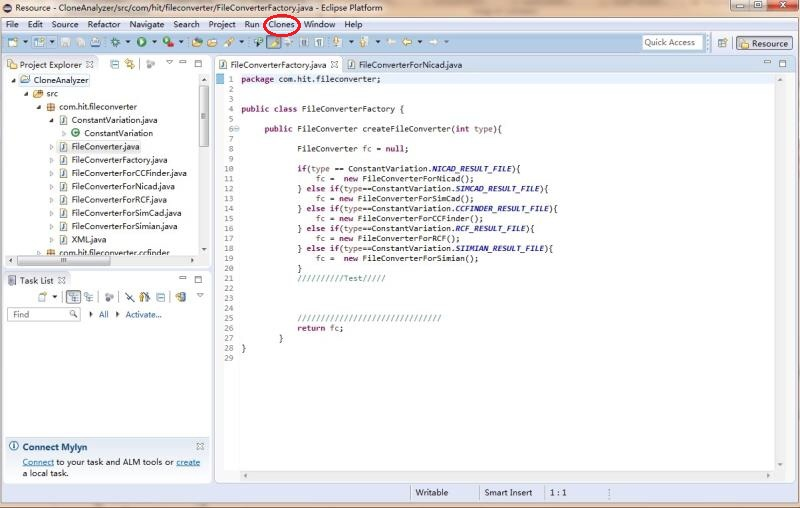
\includegraphics[width = 0.8\textwidth]{plugin1.jpg}
\bicaption[pluginview1]{}{插件安装完成后Eclipse界面}{Fig.$\!$}
{The screen-shot for eclipse with installed plug-in of clone consistency prediction}
\vspace{-1em}
\end{figure}

在使用本文所设计的一致性维护需求预测插件时,需要提前加载已训练好的机器学习模型。为方便用户使用,本章插件提供三种方式加载预测模型:(1)加载系统源代码及克隆检测工具的检测结果构建预测模型;(2)加载已有软件历史版本特征向量训练预测模型;(3)加载已有预测模型。其中特征文件目前仅支持ARFF格式文件。加载所需功能如图~\ref{pluginview2}~所示。%其中Show Clones 菜单项是显示当前通过复制粘贴形成的克隆代码、已经被程序开发人员修改的克隆代码。

\begin{figure}[htbp]
\centering
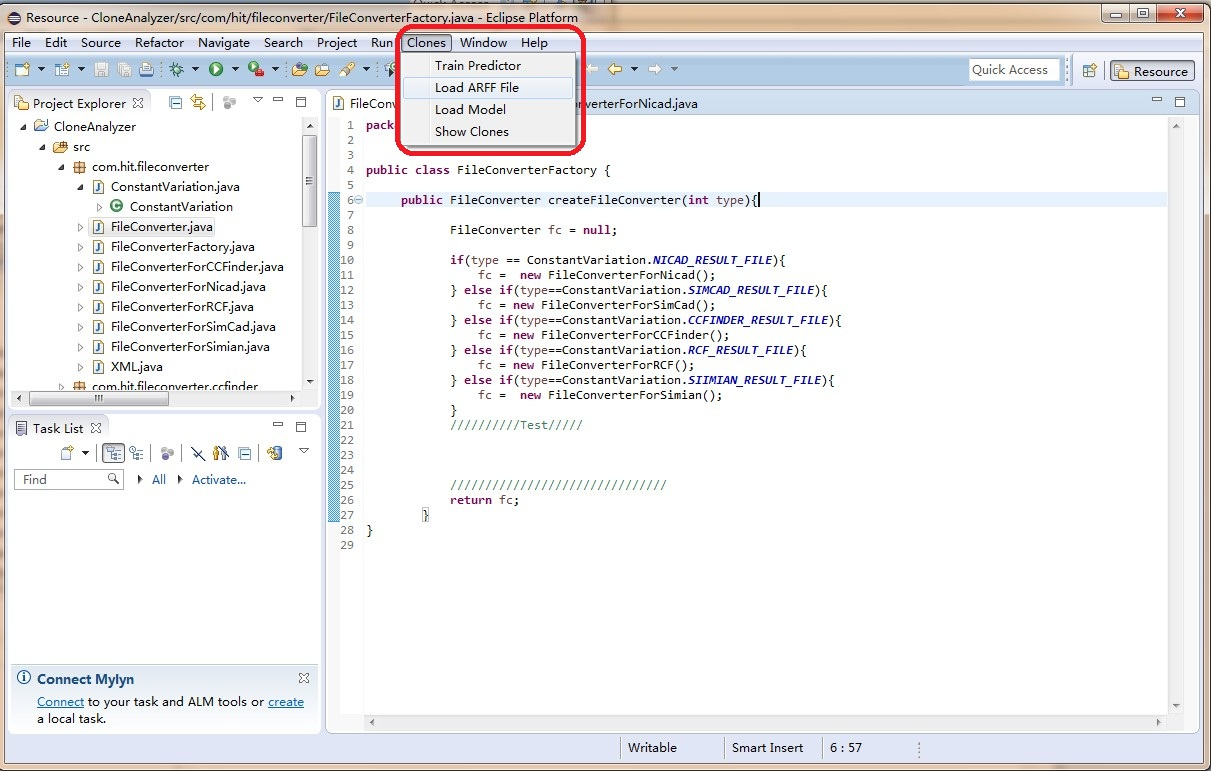
\includegraphics[width = 0.8\textwidth]{plugin2.jpg}
\bicaption[pluginview2]{}{插件加载预测模型的截图}{Fig.$\!$}
{The screen-shot for loading the models of clone consistency prediction}
\vspace{-1em}
\end{figure}


成功加载预测模型后,该插件便可以预测克隆代码的一致性维护需求。通过监听开发过程中的克隆创建和变化实例,并预测克隆代码的一致性维护需求。图中~\ref{pluginview3}~是一个会导致额外维护代价的克隆创建操作的警告实例。如图所示,本插件会警告软件开发人员,其操作会引发额外的维护代价。根据预测结果,开发人员可以采取相应的操作。


\begin{figure}[htbp]
\centering
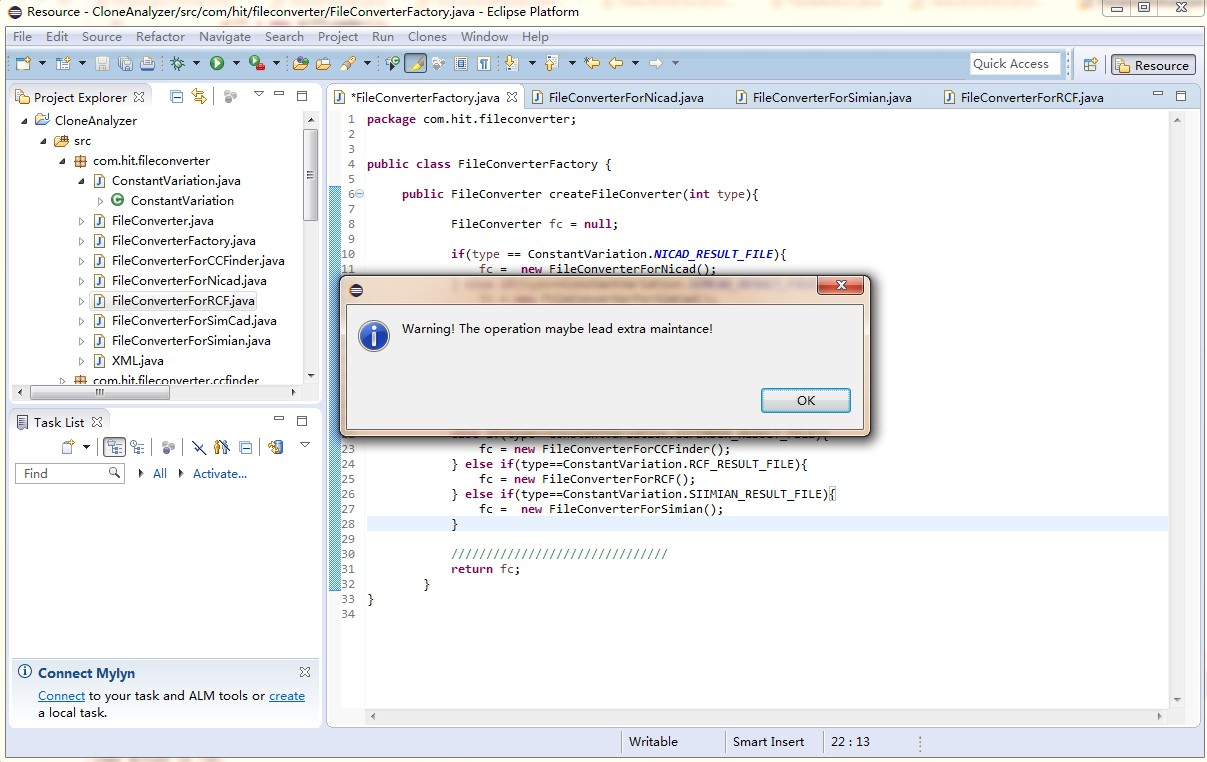
\includegraphics[width = 0.8\textwidth]{plugin3.jpg}
\bicaption[pluginview3]{}{需要一致性维护的预测结果示例}{Fig.$\!$}
{The screen-shot for a prediction example that meeting consistency}
\vspace{-1em}
\end{figure}

%%%%%当通过软件源代码和克隆检测结果加载预测模型时,需要对克隆检测结果进行处理,提取表示克隆代码的特征,并生成特征文件作为训练集,训练预测模型。该部分最初设计成一个独立的Application, 最后将其打成Jar 包嵌入到Eclipse 开发环境中。
%%%%%本节主要介绍最初的独立的Application, 以说明该模块功能。该Application的界面进行简单处理,运行界面如图2-1所示。

%%%% 
%%%% \begin{figure}[htbp]
%%%%\centering
%%%%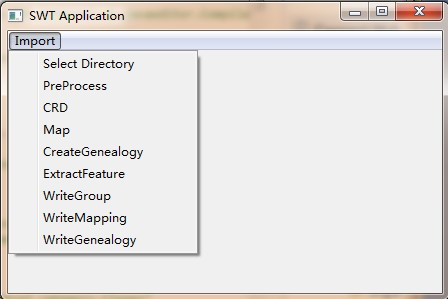
\includegraphics[width = 0.4\textwidth]{plugin4.jpg}
%%%%\bicaption[pluginview3]{}{插件安装完成后Eclipse界面}{Fig.$\!$}
%%%%{The screen-shot of eclipse after install our plug-in}
%%%%\vspace{-1em}
%%%%\end{figure}
%%%% 
%%%%图2-1 Application运行界面
%%%%主要包括五个功能,构建克隆区域描述符(CRD),构建相邻版本间克隆代码的映射关系(Map),生成克隆家系(CreateGenealogy),提取训练需要的各种特征形成特征文件(ExtractFeature),以及克隆表示的测试(WriteGroup,WriteMapping,WriteGenealogy),分别单击每一项,完成相应功能。Select Directory 项是加载软件系统源代码路径和克隆检测结果路径,其中源代码路径给到包括各种历史版本源代码的文件夹路径,如SubjectSys\_jEdit 文件夹下存放jEdit 系统的多版本源代码路径,则源代码路径给到SubjectSys\_jEdit 文件夹。克隆检测结果路径给到检测结果的上层路径,例如Nicad 的检测结果是按克隆粒度存放的,例如jEdit 系统使用Nicad 按块进行检测的结果存放形式是jEdit 文件夹下有block 文件夹,block 文件夹才存放克隆检测结果,因此路径给到jEdit文件夹 而不是block 文件夹。PreProcess 项是调用所有功能,从构建克隆代码的CRD 信息到生成特征文件。因为当系统中克隆代码过多时,调用PreProcess 结果较慢,因此将每个功能单独出来方便测试,观察结果

\BiSection{本章小结}
{Summary of this Chapter}

在软件开发过程中,克隆代码的一致性变化会增加软件维护的代价。然而,软件开发初期由于克隆实例较少,无法训练机器学习模型进行一致性预测。因此,本章在第三章和第四章研究的基础上,统一了克隆创建和变化的一致性维护需求定义,并结合软件开发过程,对跨项目的克隆代码一致性维护需求预测进行研究。在四个开源系统上进行了跨项目实验,从三个不同的角度回答了本章所提出的研究问题。跨项目的预测实验结果表明:在软件开发初期阶段,可以使用跨项目的训练数据训练机器学习模型,并应用于其它系统的克隆一致性需求预测中。同时,由于样本的不平衡性,不推荐使用SVM模型进行跨项目预测。训练集的规模会对跨项目的预测能力产生影响,建议增大训练集的规模,但是仍然无法弥补项目之间的差异性。最后,本章设计和开发了一个克隆代码一致性预测插件,可以帮助程序开发人员在实际的开发过程中预测克隆代码的一致性,帮助提高软件的可维护性和软件质量。
% !Mode:: "TeX:UTF-8" 

\BiAppendixChapter{结\quad 论}{Conclusions}

%学位论文的结论作为论文正文的最后一章单独排写,但不加章标题序号。

%结论应是作者在学位论文研究过程中所取得的创新性成果的概要总结,不能与摘要混为一谈。博士学位论文结论应包括论文的主要结果、创新点、展望三部分,在结论中应概括论文的核心观点,明确、客观地指出本研究内容的创新性成果(含新见解、新观点、方法创新、技术创新、理论创新),并指出今后进一步在本研究方向进行研究工作的展望与设想。对所取得的创新性成果应注意从定性和定量两方面给出科学、准确的评价,分(1)、(2)、(3)…条列出,宜用“提出了”、“建立了”等词叙述。

软件中克隆代码随着系统演化,克隆代码的存在以及在演化过程中会发生变化,导致软件难以理解和维护,已经成为了影响软件质量的一个重要因素。现有的研究方法中既不能客观全面的理解克隆代码,也不能有效地解决克隆代码一致性变化问题。针对以上问题,本文提出了基于软件演化的克隆代码分析与一致性维护方法,重点研究了克隆代码演化特征分析、克隆代码创建时和变化时的一致性需求预测和跨项目的克隆代码一致性预测,取得了如下创新性成果:

(1) 针对现有的克隆分析方法不能全面客观地理解克隆代码及其演化过程,提出了一个基于聚类的克隆代码演化特征分析方法。方法通过检测软件版本中的克隆代码,并构建系统克隆家系描述克隆代码的演化过程。为表示克隆代码及其演化情况,从克隆片段、克隆组和克隆家系三个不同的角度提取相应的属性值。在此基础上使用X-means聚类分析和挖掘克隆代码的演化特征。实验表明软件中存在的大部分克隆代码在其演化过程中是较为稳定的,并不会发生频繁的变化。同时,也存在一定规模的发生变化的克隆代码,其中发生一致性变化的克隆要多于不一致变化的克隆代码。

(2)针对新创建的克隆代码在其演化过程可能会引发一致性变化,从而导致额外的维护代价问题,提出了克隆代码创建时一致性维护需求预测方法。提供了一个克隆代码创建时的一致性维护需求定义,将问题转化为一个可以使用机器学习解决的分类问题。通过构建系统克隆家系并识别克隆演化模式,从系统中收集克隆创建实例用于训练机器学习模型,并提取代码属性和上下文属性表示创建的克隆代码。在四个实验系统上使用五种不同机器学习方法进行了评估,实验表明该方法以较高的准确率和召回率高效地预测克隆代码创建时的一致性维护需求。

(3)针对演化过程中的克隆代码的一致性变化可能引发的一致性缺陷问题,提出了克隆代码变化时一致性维护需求预测方法。提供了克隆代码变化时的一致性维护需求定义,将问题装化为可以应用机器学习方法解决的分类问题。通过构建系统的克隆家系和识别其演化模式,从系统中收集克隆变化实例用于训练机器学习模型。从克隆组的角度提取了代码属性、上下文属性,并同时从克隆演化的角度提取了一组演化属性共同表示克隆变化实例。在四个实验系统上使用五种不同机器学习方法进行了评估,实验表明该方法以合理的准确率和召回率有效地预测克隆代码变化使得一致性维护需求。

(4)针对软件开发初期系统缺少训练数据的情况,提出了跨项目的克隆代码一致性维护需求预测方法。统一克隆创建和变化时的一致性维护需求,为克隆一致性维护需求定义。使用训练系统训练机器学习模型,并在测试系统上进行跨项目一致性预测。同时,还结合软件开发过程,基于eclipse设计并实现了一个克隆代码一致性维护需求预测插件,可以在实际开发中帮助程序开发人员预测克隆代码的一致性维护需求。在四个实验系统上使用五种不同机器学习方法进行了实证研究,结果表明跨项目预测可以在软件开发初期进行克隆一致性预测,并给出了一些建议帮助提高跨项目的预测能力。该方法可以在软件开发过程中帮助程序开发人员边开发、边预测克隆代码的一致性维护需求。

在本文工作的基础上,还有以下工作有待于进一步研究:

(1) 在克隆变化时一致性维护需求预测中,仍然有一定的改进空间。在未来研究中,拟通过改进现有的属性表示克隆代码的真实变化,从而以更高的准确率和召回率高效的预测克隆代码的一致性维护需求。

(2)在预测跨项目的克隆一致性维护需求时,方法的预测能力尚未达到令人满意的效果。在未来的研究中,拟通过添加与项目自身相关的属性、选择更为合适的实例提高跨项目的预测能力,从而帮助缺乏训练数据的新系统进行一致性维护需求预测。

(3)在软件开发过程中,本文方法仅可以警告程序开发人员克隆代码的一致性维护需求,并没有对克隆代码进行一致性维护。在未来的研究中,拟结合程序分析技术,在需要时对克隆代码自动地进行一致性维护,从而保证克隆代码的一致性。同时,结合克隆一致性预测方法,帮助识别并修复系统中已存在的一致性缺陷,从而提高软件质量。 

%参考文献
\defaultfont
\bibliographystyle{GBT7714-2005NLang-HIT}
\addcontentsline{toc}{chapter}{参考文献}      % 参考文献加入到中文目录
\addcontentsline{toe}{chapter}{\bfseries  References} % 参考文献加入到英文目录
\addtolength{\bibsep}{-0.8em}
\nocite{*}  %若将此命令屏蔽掉,则未引用的文献不会出现在文后的参考文献列表中。
\bibliography{reference}
\renewcommand{\appendixname}{附录~\Alph{chapter}}
\renewcommand{\theequation}{\Alph{chapter}-\arabic{equation}}
\renewcommand{\thetable}{\Alph{chapter}-\arabic{table}}
%% -*-coding: utf-8 -*-

\defaultfont
\appendix

%%%%%%%%%%%%%%%%%%%%%%%%%%%%%%%%%%%%%%%%%%%%%%%%%%%%%%%%%
\BiAppChapter{带章节的附录}{Full Appendix}%
完整的附录内容,包含章节,公式,图表等

%%%%%%%%%%%%%%%%%%%%%%%%%%%%%%%%%%%%%%%%%%%%%%%%%%%%%%%%%
\BiSection{附录节的内容}{Section in Appendix}
这是附录的节的内容

附录中图的示例:
\begin{figure}[htbp]
\centering
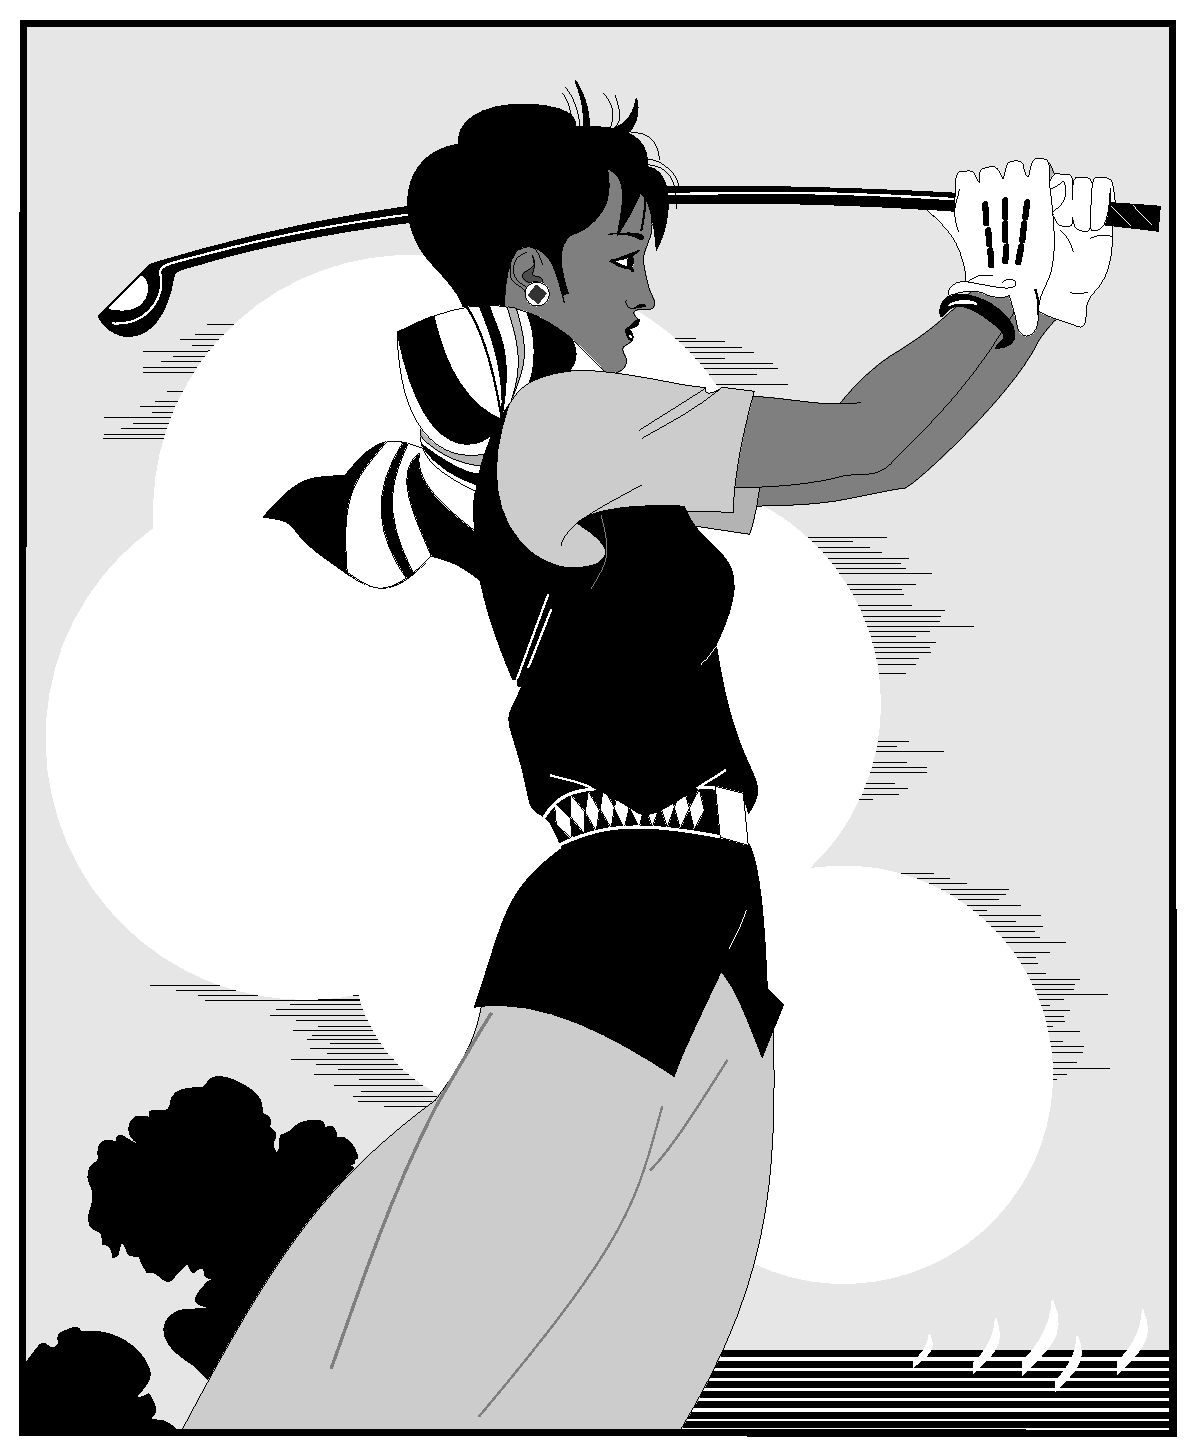
\includegraphics[width = 0.4\textwidth]{golfer}
\bicaption[golfer5]{}{打高尔夫球的人}{Fig.$\!$}{The person playing golf}\vspace{-1em}
\end{figure}

附录中公式的示例:
\begin{align}
a & = b \times c \\
E & = m c^2
\end{align}

\BiAppChapter{这个星球上最好的免费Windows软件列表}{List of the Best Free Windows Software in our Planet}
\section*{杀毒软件}
\href{http://www.avast.com/zh-cn/free-antivirus-download}{avast! 免费杀毒软件}——推荐

\href{http://www.avg.com/cn-zh/china-avg-antivirus-free}{AVG 杀毒永久免费版}——推荐

\href{http://www.avira.com/en/avira-free-antivirus}{Avira Free Antivirus (小红伞)}









%\BiAppChapter{附录三}{appendix 3}    % 附录
% !Mode:: "TeX:UTF-8" 

\BiAppendixChapter{攻读\cxuewei 学位期间发表的论文及其他成果} {Papers
published in the period of PH.D. education}
\noindent\textbf{(一)已发表的学术论文}
%\noindent\textbf{(一)已发表的(含录用)学术论文}
\begin{publist}

\item
\underline{Zhang Fanlong}, Khoo Siau-Cheng, Su Xiaohong{$^*$}. Predicting Change Consistency in A Clone Group[J]. Journal of Systems and Software. 134(2017), 105-119.
(已发表, DOI:10.1016/j.jss.2017.08.045, SCI收录,  5-Year IF=2.619, CCF推荐B类期刊, 中科院SCI期刊分区3区, 对应第4章, 第一作者)
%2016年IF=2.444, 

\item
\underline{Zhang Fanlong}, Khoo Siau-Cheng, Su Xiaohong{$^*$}. Predicting Consistent Clone Change[C]. Proceeding of the 27th International Symposium on Software Reliability Engineering (ISSRE), Ottawa, Canada, 2016: 353-364.
(已发表, DOI:10.1109/ISSRE.2016.11, EI:20170803379101, CCF推荐B类会议, 对应第4章, 第一作者)

\item
\underline{Zhang Fanlong}, Khoo Siau-cheng, Su Xiaohong{$^*$}. Machine-Learning Aided Analysis of Clone Evolution[J/OL]. Chinese Journal of Electronics(2017-09-28). http://kns.cnki.net/kcms/detail/10.1284.TN.20170928.1353.002.html.
(已发表, DOI:10.1049/cje.2017.08.012, SCI收录, 2016年IF=0.513, 中科院分区4区, 对应第2章, 第一作者)

%%%\item
%%%\underline{Zhang Fanlong}, Khoo Siau-cheng, Su Xiaohong{$^*$}. Machine-Learning Aided Analysis of Clone Evolution[J]. Chinese Journal of Electronics.  26(2017).
%%%(已发表, DOI:10.1049/cje.2017.08.012, SCI收录, 2016年IF=0.513, 中科院分区4区, 对应第2章, 第一作者)

\item
苏小红, \underline{张凡龙}{$^*$}. 面向管理的克隆代码研究综述[J/OL]. 计算机学报2017(2017-08-24). On Publishing: No.120, Vol.40. http://kns.cnki.net/kcms/detail/11.1826.TP.20170728.1305.046.html.
(已发表, EI收录, 一级学报, 对应第1章, 第二作者, 导师为第一作者)

%%%\item
%%%苏小红, \underline{张凡龙}{$^*$}. 面向管理的克隆代码研究综述[J/OL]. 计算机学报2017(2017-07-28) [2017-08-24]. http://kns.cnki.net/kcms/detail/11.1826.TP.20170728.1305.046.html.
%%%(网络优先发表, EI收录, 一级学报, 对应第1章, 第二作者, 导师为第一作者)

\item
\underline{Zhang Fanlong }, Su Xiaohong{$^*$},  Zhao Wen,  Ma Peijun. An Empirical Study of Code Clone Clustering Based on Clone Evolution[J]. Journal of Harbin Institute of Technology(New Series).2017, 24(2):10-18.
(已发表, DOI:10.11916/j.issn.1005-9113.15316, 哈工大学报英文版, 对应第2章, 第一作者)

\item
\underline{张凡龙}, 苏小红{$^*$},  李智超,  马培军. 基于支持向量机的克隆代码有害性评价方法[J]. 智能计算机与应用, 2016, 6(4): 112-115. 
(已发表, 对应第3章, 第一作者)

\item
Su Xiaohong{$^*$}, \underline{Zhang Fanlong},  Xia Li, et al. Functionally Equivalent C Code Clone Refactoring by Combining Static Analysis with Dynamic Testing[C]. Proceeding of the International Conference on Soft Computing Techniques and Engineering Application. 2014: 247-256.
(已发表, DOI: 10.1007/978-81-322-1695-7\_28, EI:20151600752325, 第二作者, 导师为第一作者)
\end{publist}

\noindent\textbf{(二)审稿中的学术论文}
\begin{publist}

\item
\underline{Zhang Fanlong},  Khoo Siau-Cheng, Su Xiaohong{$^*$}. An Empirical Study on Clone Consistency-Requirement Prediction Based on Machine Learning[J]. Journal of Computer Science and Technology.
(大修, SCI收录, 2016年IF=0.956, CCF推荐B类期刊, 中科院SCI期刊分区4区, 对应第5章, 第一作者)

\item
\underline{Zhang Fanlong}, Khoo Siau-cheng, Su Xiaohong{$^*$}. Improving Maintenance-Consistency Prediction During Code Clone Creation[J]. Software Quality Journal. 
(在审, SCI收录, 2916年IF=1.816, CCF推荐C类期刊, 中科院SCI期刊分区4区, 对应第3章, 第一作者)

\item
\underline{Zhang Fanlong }, Su Xiaohong{$^*$}. Cross-Project Clone Consistency Prediction[J]. Journal of Systems and Software.
(在审, SCI收录, 5-Year IF=2.619, 2016年IF=2.444, CCF推荐B类期刊, 中科院SCI期刊分区3区, 对应第5章, 第一作者)
%Cluster Computing. (在审, SCI收录, 2016年IF=2.040, 中科院SCI期刊分区3区, 对应第5章, 第一作者)

%\item 放弃
%\underline{Zhang Fanlong }, Su Xiaohong.  CCP: An Plug-in for Clone Consistency Prediction[C] 
%(在投, 对应第5章, 第一作者)

%\item 放弃
%\underline{张凡龙 }, 何蔷, 苏小红{$^*$}. 克隆代码可视化方法研究[J].哈尔滨工业大学学报.
% (在投, EI收录, 第一作者)

\end{publist}

\noindent\textbf{(三)与他人合作的学术论文}
\begin{publist}
\item
Yuan Yue, \underline{Zhang Fanlong},  Su Xiaohong{$^*$}. CloneAyz: An Approach for Clone Representation and Analysis[C]. Proceeding of the 3rd International Conference on Information Science and Control Engineering (ICISCE), 2016: 252-256.(已发表, EI:20165003106894, DOI:10.1109/ICISCE.2016.63, 第二作者)
\end{publist}

%%\noindent\textbf{(二)申请及已获得的专利(无专利时此项不必列出)}
%%\begin{publist}
%%\item XXX,XXX. 一种温热外敷药制备方案:中国,88105607.3[P]. 1989-07-26.
%%\end{publist}
\noindent\textbf{(四)参与的科研项目}
\begin{publist}

\item
苏小红等. 建筑全性能联合仿真平台内核开发. “十三五”国家重点研发计划课题. 课题编号:2017YFC0702204.
\item	
苏小红等. 基于启发式选择变异和软件行为特征挖掘的软件错误定位方法. 国家自然科学基金项目. 课题编号:61672191.
\item	
苏小红等. 无定型克隆代码的检测及重构方法. 国家自然科学基金项目. 课题编号:61173021.
\item
苏小红等. 数据挖掘和静态分析相结合的克隆代码缺陷检测及重构方法. 国家自然科学基金项目. 课题编号:61073052.
\item
苏小红等. 面向理解的软件错误定位方法. 国家自然科学基金项目. 课题编号:61202092.

\item
苏小红等. 基于程序转换和语义分析的编程自动评分方法研究. 国家自然科学基金项目. 课题编号:60673035.

\end{publist}
\vfill
\hangafter=1\hangindent=2em\noindent

\setlength{\parindent}{2em}
    % 所发文章
% !Mode:: "TeX:UTF-8" 

\BiAppendixChapter{哈尔滨工业大学学位论文原创性声明和使用权限}{Statement of copyright and Letter of authorization}
\vspace{\baselineskip}
\begin{center}\hei\xiaosan{学位论文原创性声明}\end{center}
\vspace{1em}

本人郑重声明:此处所提交的学位论文《\chinesethesistitle》,是本人在导师指导下,在哈尔滨工业大学攻读学位期间独立进行研究工作所取得的成果,且学位论文中除已标注引用文献的部分外不包含他人完成或已发表的研究成果。对本学位论文的研究工作做出重要贡献的个人和集体,均已在文中以明确方式注明。

\vspace{\baselineskip}
\hspace{6em}作者签名:\hfill 日期:\hspace{2.5em}年\hspace{1.5em}月\hspace{1.5em}日

\vspace{2\baselineskip}
\begin{center}\hei\xiaosan{学位论文使用权限}\end{center}
\vspace{1em}

学位论文是研究生在哈尔滨工业大学攻读学位期间完成的成果,知识产权归属哈尔滨工业大学。学位论文的使用权限如下:

(1)学校可以采用影印、缩印或其他复制手段保存研究生上交的学位论文,并向国家图书馆报送学位论文;(2)学校可以将学位论文部分或全部内容编入有关数据库进行检索和提供相应阅览服务;(3)研究生毕业后发表与此学位论文研究成果相关的学术论文和其他成果时,应征得导师同意,且第一署名单位为哈尔滨工业大学。

保密论文在保密期内遵守有关保密规定,解密后适用于此使用权限规定。

本人知悉学位论文的使用权限,并将遵守有关规定。


\vspace{2\baselineskip}
\hspace{6em}作者签名:\hfill 日期:\hspace{2.5em}年\hspace{1.5em}月\hspace{1.5em}日

\vspace{2\baselineskip}
\hspace{6em}导师签名:\hfill 日期:\hspace{2.5em}年\hspace{1.5em}月\hspace{1.5em}日   % 承诺
% !Mode:: "TeX:UTF-8" 

\BiAppendixChapter{致\quad 谢}{Acknowledgements}

在此论文完成之际,谨向给予我无私帮助和关怀的人们致以最诚挚的谢意!

衷心感谢我的导师苏小红教授!本文是在苏老师的悉心指导下完成的,几年来苏老师对我的科研工作给予了大力支持,也在日常生活等等方面给予了无微不至的关怀。在攻读博士期间,论文的选题、开题、中期以及博士论文撰写的各个阶段,苏老师给予了细致且精心的指导,在此向她表达最衷心的感谢,她的言传身教将使我终生受益。苏老师渊博的知识、远见的学术洞察力、严谨的治学态度和执着的敬业精神使我受益匪浅。没有苏老师的悉心指导和热情鼓励,我的博士论文工作不可能如此顺利的完成。在此,谨向恩师致以由衷的敬意和衷心的感谢!

衷心感谢新加坡国立大学的Khoo Siau-Cheng教授!在新加坡国立大学访学期间,Prof. Khoo悉心地指导我进行学术研究,细致地与我讨论学术问题,认真的帮我修改学术论文。Prof. Khoo严谨的治学态度、卓越的学术能力将是我终生学习的方向!

衷心感谢所有对本文提出宝贵意见的专家们,尤其是责任专家、外审专家以及答辩专家!在所有专家的帮助、批评和指正下,使得本文更加完善。

衷心感谢实验室全体老师和同窗们的热情帮助和支持!感谢王甜甜老师、张彦航老师、赵玲玲老师!感谢实验室的师兄师姐师弟师妹们!

衷心感谢我的父母!感谢他们将我抚养成人,尽力的创造最好的条件和资源让我接受最好的教育,是他们对我一直以来的支持、关心、理解和厚望,鼓励和激励着我全身心的投入学习,让我有了最坚实的后盾,在遇到困难时从而能有继续前行的决心、勇气和动力。

衷心感谢我的女朋友王子萍!感谢她在我博士最后阶段的陪伴,在我沮丧、失落时一次次地鼓励和安慰我!

博士只是人生不断学习的一个阶段,我将继续开启新的人生。以一句话勉励自身:“天行健,君子以自强不息;地势坤,君子以厚德载物!”
% 致谢

\ifxueweidoctor
% !Mode:: "TeX:UTF-8" 

\defaultfont

\BiAppendixChapter{个人简历}{Resume}

张凡龙,男,生于1987~年~11~月~06~日,山东省兖州市人。

2006~年~09~月------2010~年~07~月,就读于~东北林业大学~信息与工程学院~计算机科学与技术专业~,并获得~工~学学士学位。

2010~年~09~月------2012~年~07~月,就读于~哈尔滨工业大学~计算机科学与技术学院~计算机科学与技术学科~,并获得~工~学硕士学位。

2015~年~08~月------2016~年~08~月,于~新加坡国立大学~计算学院~计算机科学系~访问,Visiting Student。

2012~年~09~月------至今,就读于~哈尔滨工业大学~计算机科学与技术学院~计算机科学与技术学科~,攻读博士学位。

%获奖情况:如获三好学生、优秀团干部、X~奖学金等(不含科研学术获奖)。

%工作经历:

%研究兴趣与领域
主要研究领域为软件工程、程序分析、克隆代码、软件仓库挖掘等。

在攻读学位博士期间,发表(含在审)论文11篇,其中SCI期刊5篇,国内一级学报2篇,国际会议3篇,国内期刊2篇。%,至今SCI收录2篇,EI收录4篇。

\vspace{3em}\noindent
%\textbf{( 除全日制硕士生以外,其余学生均应增列此项。个人简历一般应包含教育经历和工作经历。)}          % 博士学位论文有个人简介
\fi

\clearpage

\end{document} 